\documentclass[krantz2]{krantz}\usepackage{knitr}%,ChapterTOCs

%\usepackage[utf8]{inputenc}
\usepackage{color}

\usepackage{polyglossia}
\setdefaultlanguage[variant = british, ordinalmonthday = false]{english}

%\usepackage{gitinfo2} % remember to setup Git hooks

\usepackage{hologo}

\usepackage{csquotes}

\usepackage{graphicx}
\DeclareGraphicsExtensions{.jpg,.pdf,.png}

\usepackage{animate}

%\usepackage{microtype}
\usepackage[style=authoryear-comp,giveninits,sortcites,maxcitenames=2,%
    mincitenames=1,maxbibnames=10,minbibnames=10,backref,uniquename=mininit,%
    uniquelist=minyear,sortgiveninits=true,backend=biber]{biblatex}%,refsection=chapter

\newcommand{\href}[2]{\emph{#2} (\url{#1})}

%\usepackage[unicode,hyperindex,bookmarks,pdfview=FitB,%backref,
%            pdftitle={Learn R ...as you learnt your mother tongue},%
%            pdfkeywords={R, statistics, data analysis, plotting},%
%            pdfsubject={R},%
%            pdfauthor={Pedro J. Aphalo}%
%            ]{hyperref}

%\hypersetup{colorlinks,breaklinks,
%             urlcolor=blue,
%             linkcolor=blue,
%             citecolor=blue,
%             filecolor=blue,
%             menucolor=blue}

\usepackage{framed}

\usepackage{abbrev}
\usepackage{usingr}

\usepackage{imakeidx}

% this is to reduce spacing above and below verbatim, which is used by knitr
% to show returned values
\usepackage{etoolbox}
\makeatletter
\preto{\@verbatim}{\topsep=-5pt \partopsep=-4pt \itemsep=-2pt}
\makeatother

%%% Adjust graphic design

% New float "example" and corresponding "list of examples"
%\DeclareNewTOC[type=example,types=examples,float,counterwithin=chapter]{loe}
%\DeclareNewTOC[name=Box,listname=List of Text Boxes, type=example,types=examples,float,counterwithin=chapter,%
%]{lotxb}

% changing the style of float captions
%\addtokomafont{caption}{\sffamily\small}
%\setkomafont{captionlabel}{\sffamily\bfseries}
%\setcapindent{0em}

% finetuning tocs
%\makeatletter
%\renewcommand*\l@figure{\@dottedtocline{1}{0em}{2.6em}}
%\renewcommand*\l@table{\@dottedtocline{1}{0em}{2.6em}}
%\renewcommand*\l@example{\@dottedtocline{1}{0em}{2.3em}}
%\renewcommand{\@pnumwidth}{2.66em}
%\makeatother
%
%% add pdf bookmarks to tocs
%\makeatletter
%\BeforeTOCHead{%
%  \cleardoublepage
%    \edef\@tempa{%
%      \noexpand\pdfbookmark[0]{\list@fname}{\@currext}%
%    }\@tempa
%}

\setcounter{topnumber}{3}
\setcounter{bottomnumber}{3}
\setcounter{totalnumber}{4}
\renewcommand{\topfraction}{0.90}
\renewcommand{\bottomfraction}{0.90}
\renewcommand{\textfraction}{0.10}
\renewcommand{\floatpagefraction}{0.70}
\renewcommand{\dbltopfraction}{0.90}
\renewcommand{\dblfloatpagefraction}{0.70}

\addbibresource{rbooks.bib}
\addbibresource{references.bib}

\makeindex[title=General index]
\makeindex[name=rindex,title=Alphabetic index of \Rlang names]
\makeindex[name=rcatsidx,title=Index of \Rlang names by category]
\IfFileExists{upquote.sty}{\usepackage{upquote}}{}
\begin{document}

% customize chapter format:
%\KOMAoption{headings}{twolinechapter}
%\renewcommand*\chapterformat{\thechapter\autodot\hspace{1em}}

% customize dictum format:
%\setkomafont{dictumtext}{\itshape\small}
%\setkomafont{dictumauthor}{\normalfont}
%\renewcommand*\dictumwidth{0.7\linewidth}
%\renewcommand*\dictumauthorformat[1]{--- #1}
%\renewcommand*\dictumrule{}

%\extratitle{\vspace*{2\baselineskip}%
%             {\Huge\textsf{\textbf{Learn R}\\ \textsl{\huge\ldots as you learnt your mother tongue}}}}

\title{\Huge{\fontseries{ub}\sffamily Learn R\\{\Large\ldots as you learnt your mother tongue}}}

%\subtitle{Git hash: \gitAbbrevHash; Git date: \gitAuthorIsoDate}

\author{Pedro J. Aphalo}

\date{Helsinki, \today}

%\publishers{Draft, 95\% done\\Available through \href{https://leanpub.com/learnr}{Leanpub}}

%\uppertitleback{\copyright\ 2001--2017 by Pedro J. Aphalo\\
%Licensed under one of the \href{http://creativecommons.org/licenses/}{Creative Commons licenses} as indicated, or when not explicitly indicated, under the \href{http://creativecommons.org/licenses/by-sa/4.0/}{CC BY-SA 4.0 license}.}
%
%\lowertitleback{Typeset with \href{http://www.latex-project.org/}{\hologo{XeLaTeX}}\ in Lucida Bright and \textsf{Lucida Sans} using the KOMA-Script book class.\\
%The manuscript was written using \href{http://www.r-project.org/}{R} with package knitr. The manuscript was edited in \href{http://www.winedt.com/}{WinEdt} and \href{http://www.rstudio.com/}{RStudio}.
%The source files for the whole book are available at \url{https://bitbucket.org/aphalo/using-r}.}

%\frontmatter

% knitr setup

















% \thispagestyle{empty}
% \titleLL
% \clearpage

\frontmatter

\maketitle

%\begin{titlingpage}
%  \maketitle
%\titleLL
%\end{titlingpage}

\setcounter{page}{7} %previous pages will be reserved for frontmatter to be added in later.
\tableofcontents
%\chapter*{Foreword}
I am delighted to introduce the first book on Multimedia Data Mining.  When I came to know about this book project undertaken by two of the most active young researchers in the field, I was pleased that this book is coming in early stage of a field that will need it more than most fields do.  In most emerging research fields, a book can play a significant role in bringing some maturity to the field.  Research fields advance through research papers.  In research papers, however, only a limited perspective could be provided about the field, its application potential, and the techniques required and already developed in the field.  A book gives such a chance.  I liked the idea that there will be a book that will try to unify the field by bringing in disparate topics already available in several papers that are not easy to find and understand.  I was supportive of this book project even before I had seen any material on it.  The project was a brilliant and a bold idea by two active researchers.  Now that I have it on my screen, it appears to be even a better idea.  

Multimedia started gaining recognition in 1990s as a field.  Processing, storage, communication, and capture and display technologies had advanced enough that researchers and technologists started building approaches to combine information in multiple types of signals such as audio, images, video, and  text.  Multimedia computing and communication techniques recognize correlated information in multiple sources as well as insufficiency of information in any individual source.    By properly selecting sources to provide complementary information, such systems aspire, much like human perception system, to create a holistic picture of a situation using only partial information from separate sources.

Data mining is a direct outgrowth of progress in data storage and processing speeds.  When it became possible to store large volume of data and run different statistical computations to explore all possible and even unlikely correlations among data, the field of data mining was born.  Data mining allowed people to hypothesize relationships among data entities and explore support for those.  This field has been put to applications in many diverse domains and keeps getting more applications.  In fact many new fields are direct outgrowth of data mining and it is likely to become a powerful computational tool.\vadjust{\vfill\pagebreak}



\chapter*{Preface}

\begin{VF}
``Suppose that you want to teach the `cat' concept to a very young child. Do you explain that a cat is a relatively small, primarily carnivorous mammal with retractible claws, a distinctive sonic output, etc.? I'll bet not. You probably show the kid a lot of different cats, saying `kitty' each time, until it gets the idea. To put it more generally, generalizations are best made by abstraction from experience.''

\VA{R. P. Boas}{Can we make mathematics intelligible?}
\end{VF}

%\dictum[R. P. Boas (1981) Can we make mathematics intelligible?, \emph{American Mathematical Monthly} \textbf{88:} 727-731.]{"Suppose that you want to teach the `cat' concept to a very young child. Do you explain that a cat is a relatively small, primarily carnivorous mammal with retractible claws, a distinctive sonic output, etc.? I'll bet not. You probably show the kid a lot of different cats, saying `kitty' each time, until it gets the idea. To put it more generally, generalizations are best made by abstraction from experience."}


% Such pauses are not a miss use of our time. To learn a natural language we need to interact with other speakers, we need feedback. In the case of R, we can get feedback both from the outcomes from our utterances to the computer, and from other \Rlang users.}
\noindent
This book covers different aspects of the use of the \Rlang language. Chapters \ref{chap:R:introduction} to \ref{chap:R:functions} describe the \Rlang language itself. Later chapters describe extensions to the \Rlang language available through contributed \emph{packages}, the \emph{grammar of data} and the \emph{grammar of graphics}. In this book, explanations are concise but contain pointers to additional sources of information, so as to encourage the development of a routine of independent exploration. This is not an arbitrary decision, this is the normal \emph{modus operandi} of most of us who use \Rlang regularly for a variety of different problems. Some have called approaches like the one used here, ``learning the hard way'', but I would call it ``learning to be independent''.

I do not discuss in this book statistics or data analysis methods, I describe \Rlang as a language for data manipulation and display. The idea is for you to learn the \Rlang language in a way comparable to how children learn a language: they work-out what the rules are, simply by listening to people speak and trying to utter what they want to tell their parents. Of course, small children receive some guidance, but are not taught a prescriptive set of rules like when learning a second language at school. Instead of listening, you will read code and instead of speaking you will try to execute \Rlang  code statements on a computer---i.e. you will try your hand at using \Rlang to tell a computer what you want it to compute. I do provide explanations and guidance, but the idea of this book is for you to use the numerous examples to find-out by yourself the overall patterns and coding philosophy behind the \Rlang language. Instead of parents being the sound board for your first utterances in \Rlang, the computer will play this role. You will \emph{play} by modifying the examples, see how the computer responds, does \Rlang understand you or not? Using actively a language is the most efficient way of learning it. By using it, I mean actually reading, writing and running scripts or programs (copying and pasting, or typing ready-made examples from books or the internet does not qualify as using a language).

What is a language? A language is a system of communication. \Rlang as a language allows us to communicate with other members of the \Rlang community, and with computers. As most languages in active use, \Rlang evolves. New ``words'' and new ``constructs'' are incorporated into the language, and some earlier frequently used ones are relegated to the fringes of the corpus. I describe current usage and ``modisms'' of the \Rlang language in a way accessible to a readership unfamiliar with computer science but with some background in data analysis as used in Biology, Engineering, or Humanities.

When teaching I tend to lean towards challenging students rather than telling an over-simplified story. There are two reasons for this. First, I prefer as a student, and I learn best myself if the going is not too easy. Second, if I would hide the tricky bits of the \Rlang language, it would make readers' life much more difficult later on. You, will not remember all the details, nobody could. However, you most likely will remember in which situations you need to be careful or should check the details. So, I will expose you not only the usual cases, but also to several exceptions and counterintuitive features of the language. Reading this book will be about exploring a new world, this book aims to be a travel guide, but neither a traveler's account, nor a cookbook of \Rlang recipes.

Keep in mind that it is impossible to remember everything about \Rlang! The \Rlang language in a broad sense is vast because its capabilities can be expanded with independently developed packages. Learning to use \Rlang consists in learning the basics plus developing the skill of finding your way in \Rlang and its documentation.  In 2017 the number packages available in the Comprehensive \Rlang Archive Network (CRAN) broke the 10\,000 barrier. CRAN is the most important, but not only, public repository for \Rlang packages. How good a command of the \Rlang language and packages a user needs depends on the type activities to be carried out. This book attempts to train you in the use of the \Rlang language itself and of popular \Rlang language extensions for data manipulation and graphical display. Given the availability of numerous books on statistical analysis with \Rlang, in the present book I will cover only the bare minimum of this subject. The same is true for package development in \Rlang. This book seats in-between, aiming at teaching programming in-the-small: the use of \Rlang to automate the drudgery of data manipulation from raw data, through data exploration to the production of publication quality illustrations.

As with all ``rich'' languages there are many different ways of doing things in \Rlang, and there is in almost all cases no one-size-fits-all solution to a problem. There is always a compromise involved, usually between time spent by the user and processing time required in the computer. Many of the packages that are most popular nowadays did not exist when I started using \Rlang, and many of these packages make new approaches available. One could write many different \Rlang books with a given aim using substantially different ways of achieving the same results. In this book, I limit myself to packages that are currently popular and/or that I consider elegantly designed. I have in particular tried to limit myself to packages with similar design philosophies, especially in relation to their interfaces. What is elegant design, and in particular what is a friendly user interface depends strongly on each user's preferences and previous experience. Consequently, the contents of the book are strongly biased by my own preferences. I have tried to write examples in ways that execute fast without compromising readability. I encourage readers to take this book as a starting point for exploring the very many packages, styles and approaches which I have not described.

I will appreciate suggestions for further examples, notification of errors and unclear sections. Many of the examples here have been collected from diverse sources over many years and because of this not all sources are acknowledged. If you recognize any example as yours or someone else's please let me know so that I can add a proper acknowledgement. I warmly thank the students that over the years have asked the questions and posed the problems that have helped me write this text and correct the mistakes and voids of previous versions. I have also received help on on-line forums and in person from numerous people, learnt from archived e-mail list messages, blog posts, books, articles, tutorials, webinars, and by struggling to solve some new problems on my own. In many ways this text owes much more to people who are not authors than to myself. However, as I am the one who has written this version and decided what to include and exclude, as author, I take full responsibility for any errors and inaccuracies.

I have been using \Rlang since around 1998 or 1999, but I am still constantly learning new things about \Rlang itself and \Rlang packages. With time it has replaced in my work as a researcher and teacher several other pieces of software: \pgrmname{SPSS}, \pgrmname{Systat}, \pgrmname{Origin}, \pgrmname{Excel}, and it has become a central piece of the tool set I use for producing lecture slides, notes, books and even web pages. This is to say that it is the most useful piece of software and programming language I have ever learnt to use. Of course, in time it will be replaced by something better, but at the moment it is a key language to learn for anybody with a need to analyse and display data.

Why the title ``\emph{Learn R \ldots as you learnt your mother tongue}''? On one hand, because this book is based on exploration and practice. On the other hand, because you will be exposed to current usage and not spared the quirks of the language. When we use our mother tongue in everyday life we do not think about grammar rules or sentence structure, except for the trickier or unfamiliar situations. My aim is for this book to help you grow to use \Rlang in this same way.

\begin{framed}
\noindent\large%
\textbf{I encourage you to approach R, like a child approaches his or hers mother tongue when learning to speak:} Do not struggle, just play! If going gets difficult and frustrating, take a break! If you get a new insight, take a break to enjoy the victory!
\end{framed}

\newpage

\begin{framed}
\noindent
\textbf{Icons used to mark different content.} Throughout the book text boxes marked with icons present different types of information. First of all, we have \emph{playground} boxes indicated with \playicon\ which contain open-ended exercises---ideas and pieces of \Rlang code to play with at the \Rlang console. A few of these will require more time to grasp, and are indicated with \advplayicon. Boxes providing general information, usually not directly related to \Rlang as a language, are indicated with \infoicon. Some boxes highlighted with \ilAttention\ give important bits of information that must be remembered when using \Rlang---i.e.\ explain some unusual feature of the language. Finally, some boxes indicated by \ilAdvanced\ give in depth explanations, that may require you to spend time thinking, which en general can be skipped on first reading, but to which you should return at a later, and peaceful, time with a cup of coffee or tea.
\end{framed}
\newpage

%\newpage
%\begin{infobox}
%\noindent
%\textbf{Status as of 2016-11-23.} I have updated the manuscript to track package updates since the previous version uploaded six months ago, and added several examples of the new functionality added to packages \ggpmisc, \ggrepel, and \ggplot. I have written new sections on packages \viridis, \pkgname{gganimate}, \pkgname{ggstance}, \pkgname{ggbiplot}, \pkgname{ggforce}, \pkgname{ggtern} and \pkgname{ggalt}. Some of these sections are to be expanded, and additional sections are planned for other recently released packages.
%
%With respect to the chapter \textit{Storing and manipulating data with R} I have put it on hold, except for the introduction, until I can see a soon to be published book covering the same subject. Hadley Wickham has named the set of tools developed by him and his collaborators as \textit{tidyverse} to be described in the book titled \textit{R for Data Science} by Grolemund and Wickham (O'Reilly).
%
%An important update to \ggplot was released last week, and it includes changes to the behavior of some existing functions, specially faceting has become extensible through other packages. Several of the new facilities are described in the updated text and code included in this book and this pdf has been generated with up-to-date version of \ggplot and packages as available today from CRAN, except for \pkgname{ggtern} which was downloaded from Bitbucket minutes ago.
%
%The present update adds about 100 pages to the previous versions. I expect to upload a new update to this manuscript in one or two months time.
%
%\textbf{Status as of 2017-01-17.} Added ``playground'' exercises to the chapter describing \ggplot, and converted some of the examples earlier part of the main text into these playground items. Added icons to help readers quickly distinguish playground sections (\textcolor{blue}{\noticestd{"0055}}), information sections (\textcolor{blue}{\modpicts{"003D}}), warnings about things one needs to be specially aware of (\colorbox{yellow}{\typicons{"E136}}) and boxes with more advanced content that may require longer time/more effort to grasp (\typicons{"E04E}). Added to the sections \code{scales} and examples in the \ggplot chapter details about the use of colors in \Rlang and \ggplot2. Removed some redundant examples, and updated the section on \code{plotmath}. Added terms to the alphabetical index. Increased line-spacing to avoid uneven spacing with inline code bits.
%
%\textbf{Status as of 2017-02-09.} Wrote section on ggplot2 themes, and on using system- and Google fonts in ggpplots with the help of package \pkgname{showtext}. Expanded section on \ggplot's \code{annotation}, and revised some sections in the ``R scripts and Programming'' chapter. Started writing the data chapter. Wrote draft on writing and reading text files. Several other smaller edits to text and a few new examples.
%
%\textbf{Status as of 2017-02-14.} Wrote sections on reading and writing MS-Excel files, files from statistical programs such as SPSS, SyStat, etc., and NetCDF files. Also wrote sections on using URLs to directly read data, and on reading HTML and XML files directly, as well on using JSON to retrieve measured/logged data from IoT (internet of things) and similar intelligent physical sensors, micro-controller boards and sensor hubs with network access.
%
%\textbf{Status as of 2017-03-25.} Revised and expanded the chapter on plotting maps, adding a section on the manipulation and plotting of image data. Revised and expanded the chapter on extensions to \pkgname{ggplot2}, so that there are no longer empty sections. Wrote short chapter ``If and when \Rlang needs help''. Revised and expanded the ``Introduction'' chapter. Added index entries, and additional citations to literature.
%
%\textbf{Status as of 2017-04-04.} Revised and expanded the chapter on using \Rpgrm as a calculator. Revised and expanded the ``Scripts'' chapter. Minor edits to ``Functions'' chapter. Continued writing chapter on data, writing a section on \Rlang native apply functions and added preliminary text for a pipes and tees section. Write intro to `tidyverse' and grammar of data manipulation. Added index entries, and a few additional citations to the literature. Spell checking.
%
%\textbf{Status as of 2017-04-08.} Completed writing first draft of chapter on data, writing all the previously missing sections on the ``grammar of data manipulation''. Wrote two extended examples in the same chapter. Add table listing several extensions to \pkgname{ggplot2} not described in the book.
%
%\textbf{Status as of 2017-04-13.} Revised all chapters correcting some spelling mistakes, adding some explanatory text and indexing all functions and operators used. Thoroughly revised the Introduction chapter and the Preface. Expanded section on bar plots (now bar and column plots). Revised section on tile plots. Expanded section on factors in chapter 2, adding examples of reordering of factor labels, and making clearer the difference between the labels of the levels and the levels themselves.
%
%\textbf{Status as of 2017-04-29.} Tested with R 3.4.0. Package \pkgname{gganimate} needs to be installed from Github as the updated version is not yet in CRAN. Function \code{gg\_animate()} has been renamed \code{gganimate().}
%
%\textbf{Status as of 2017-05-14.} Submitted package \pkgname{learnrbook} to CRAN. Revised code in the book
%to use this new package. Small fixes after more testing. Added examples of plotting and labeling based on fits with \code{method = "nls"}, including use of the new \code{ggpmisc::stat\_fit\_tidy()}.
%
%\textbf{Status as of 2017-06-11.} Added sections on R-code bench marking and profiling for performance optimization. Added also an example of explicit compilation of a function defined in the R language. Added section on functions \code{assign()}, \code{get()} and \code{mget()}.
%
%\textbf{Status as of 2017-08-12.} Various edits to all chapters. Expanded section on \pkgname{ggpmisc} to include the new functionality added in version 0.2.15.9002: \code{geom\_table} and \code{stat\_fit\_tb}. Added section on package \pkgname{ggbeeswarm}. Added sections on packages \pkgname{magick} and on using \pgrmname{ImageJ} from \Rpgrm. Improved indexing and cross references.
%
%\textbf{Status as of 2017-10-25.} Edited the chapter on using R as a calculator, adding examples on insertion and deletion of members of lists and vectors, and also of use of \code{gl()} and \code{reorder()}. Edited sections on scale limits and added new section on coordinate limits to explain more thoroughly their differences and uses in chapter on plotting with \pkgname{ggplot2}. Added a section on package \pkgname{ggsignif} to the chapter on extensions to \pkgname{ggplot2}. Expanded section on \pkgname{ggpmisc} in the same chapter describing new functionality added in version 0.2.16.
%\pkgname{ggplo2} $>=$ 2.2.1.9000 is required by the current development version of \pkgname{ggpmisc}.
%
%\textbf{Status as of 2017-10-30.}  Add section on using pipes with \code{ggplot()} and layers.
%\end{infobox} 
\listoffigures
\listoftables
%%%\twocolumn
\chapter*{Contributors}

\begin{multicols}{2}
\contributor{Michael Aftosmis}{NASA Ames Research Center}{Moffett Field, California}

\contributor{Pratul K. Agarwal}{Oak Ridge National Laboratory}{Oak Ridge, Tennessee}

\contributor{Sadaf R. Alam}{Oak Ridge National Laboratory}{Oak Ridge, Tennessee}

\contributor{Gabrielle Allen}{Louisiana State University}{Baton Rouge, Louisiana}

\contributor{Martin Sandve Aln{\ae}s}{Simula Research Laboratory and University of Oslo, Norway}{Norway}

\contributor{Steven F. Ashby} {Lawrence Livermore National Laboratory}{Livermore, California}

\contributor{David A. Bader} {Georgia Institute of Technology}{Atlanta, Georgia}

\contributor{Benjamin Bergen} {Los Alamos National Laboratory}{Los Alamos, New Mexico}

\contributor{Jonathan W. Berry} {Sandia National Laboratories}{Albuquerque, New Mexico}

\contributor{Martin Berzins}{University of Utah}{Salt Lake City, Utah}

\contributor{Abhinav Bhatele}{University of Illinois}{Urbana-Champaign, Illinois}

\contributor{Christian Bischof} {RWTH Aachen University}{Germany}

\contributor{Rupak Biswas} {NASA Ames Research Center}{Moffett Field, California}\vspace*{5pt}

\contributor{Eric Bohm} {University of Illinois}{Urbana-Champaign, Illinois}\vspace*{5pt}

\contributor{James Bordner} {University of California, San Diego}{San Diego, California}\vspace*{5pt}

\contributor{George Bosilca} {University of Tennessee}{Knoxville, Tennessee}\vspace*{5pt}

\contributor{Greg L. Bryan} {Columbia University}{New York, New York}\vspace*{5pt}

\contributor{Marian Bubak} {AGH University of Science and Technology}{
Krak{\'o}w, Poland}\vspace*{5pt}

\contributor{Andrew Canning}{Lawrence Berkeley National
Laboratory}{Berkeley, California}

\contributor{Jonathan Carter} {Lawrence Berkeley National
Laboratory}{Berkeley, California}

\contributor{Zizhong Chen} {Jacksonville State University}{Jacksonville,
Alabama}

\contributor{Joseph R. Crobak} {Rutgers, The State University of New
Jersey}{Piscataway, New Jersey}

\contributor{Roxana E. Diaconescu} {Yahoo! Inc.}{Burbank, California}

\contributor{Peter Diener}
{Louisiana State University}{Baton Rouge, Louisiana}

\contributor{Jack J. Dongarra} {University of Tennessee, Knoxville, 
Oak Ridge National Laboratory, and}{University of Manchester}

\contributor{John B. Drake} {Oak Ridge National Laboratory}{Oak Ridge,
Tennessee}

\contributor{Kelvin K. Droegemeier} {University of Oklahoma}{Norman,
Oklahoma}

\contributor{St{\'e}phane Ethier} {Princeton University}{Princeton, New
Jersey}

\contributor{Christoph Freundl}
{Friedrich--Alexander--Universit{\"a}t}{Erlangen, Germany}

\contributor{Karl F{\"u}rlinger} {University of Tennessee}{Knoxville,
Tennessee}

\contributor{Al Geist} {Oak Ridge National Laboratory}{Oak Ridge,
Tennessee}

\contributor{Michael Gerndt} {Technische Universit{\"a}t
M{\"u}nchen}{Munich, Germany}

\contributor{Tom Goodale}
{Louisiana State University}{Baton Rouge, Louisiana}

\contributor{Tobias Gradl}
{Friedrich--Alexander--Universit{\"a}t}{Erlangen, Germany}

\contributor{William D. Gropp} {Argonne National Laboratory}{Argonne,
Illinois}

\contributor{Robert Harkness} {University of California, San
Diego}{San Diego, California}

\contributor{Albert Hartono} {Ohio State University}{Columbus, Ohio}

\contributor{Thomas C. Henderson} {University of Utah}{Salt Lake City,
Utah}

\contributor{Bruce A. Hendrickson} {Sandia National
Laboratories}{Albuquerque, New Mexico}

\contributor{Alfons G. Hoekstra} {University of Amsterdam}{Amsterdam,
The Netherlands}

\contributor{Philip W. Jones} {Los Alamos National Laboratory}{Los
Alamos, New Mexico}

\contributor{Laxmikant Kal{\'e}} {University of
Illinois}{Urbana-Champaign, Illinois}

\contributor{Shoaib Kamil} {Lawrence Berkeley National
Laboratory}{Berkeley, California}

\contributor{Cetin Kiris} {NASA Ames Research Center}{Moffett Field,
California}

\contributor{Uwe K{\"u}ster} {University of Stuttgart}{Stuttgart,
Germany}

\contributor{Julien Langou} {University of Colorado}{Denver, Colorado}

\contributor{Hans Petter Langtangen}
{Simula Research Laboratory and}{University of Oslo, Norway}

\contributor{Michael Lijewski} {Lawrence Berkeley National
Laboratory}{Berkeley, California}

\contributor{Anders Logg}
{Simula Research Laboratory and}{University of Oslo, Norway}

\contributor{Justin Luitjens} {University of Utah}{Salt Lake City, Utah}

\contributor{Kamesh Madduri} {Georgia Institute of Technology}{Atlanta,
Georgia}

\contributor{Kent-Andre Mardal}
{Simula Research Laboratory and}{University of Oslo, Norway}

\contributor{Satoshi Matsuoka} {Tokyo Institute of Technology}{Tokyo,
Japan}

\contributor{John M. May} {Lawrence Livermore National
Laboratory}{Livermore, California}

\contributor{Celso L. Mendes} {University of Illinois}{Urbana-Champaign,
Illinois}

\contributor{Dieter an Mey} {RWTH Aachen University}{Germany}

\contributor{Tetsu Narumi} {Keio University}{Japan}

\contributor{Michael L. Norman} {University of California, San
Diego}{San Diego, California}

\contributor{Boyana Norris} {Argonne National Laboratory}{Argonne,
Illinois}

\contributor{Yousuke Ohno} {Institute of Physical and Chemical Research
(RIKEN)}{Kanagawa, Japan}

\contributor{Leonid Oliker} {Lawrence Berkeley National
Laboratory}{Berkeley, California}

\contributor{Brian O'Shea} {Los Alamos National Laboratory}{Los Alamos,
New Mexico}

\contributor{Christian D. Ott}
{University of Arizona}{Tucson, Arizona}

\contributor{James C. Phillips} {University of
Illinois}{Urbana-Champaign, Illinois}

\contributor{Simon Portegies Zwart} {University of
Amsterdam,}{Amsterdam, The Netherlands}

\contributor{Thomas Radke}
{Albert-Einstein-Institut}{Golm, Germany}

\contributor{Michael Resch} {University of Stuttgart}{Stuttgart,
Germany}

\contributor{Daniel Reynolds} {University of California, San Diego}{San
Diego, California}

\contributor{Ulrich R{\"u}de}
{Friedrich--Alexander--Universit{\"a}t}{Erlangen, Germany}

\contributor{Samuel Sarholz}
{RWTH Aachen University}{Germany}

\contributor{Erik Schnetter}
{Louisiana State University}{Baton Rouge, Louisiana}

\contributor{Klaus Schulten} {University of Illinois}{Urbana-Champaign,
Illinois}

\contributor{Edward Seidel}
{Louisiana State University}{Baton Rouge, Louisiana}

\contributor{John Shalf} {Lawrence Berkeley National
Laboratory}{Berkeley, California}

\contributor{Bo-Wen Shen} {NASA Goddard Space Flight Center}{Greenbelt,
Maryland}

\contributor{Ola Skavhaug}
{Simula Research Laboratory and}{University of Oslo, Norway}

\contributor{Peter M.A. Sloot} {University of Amsterdam}{Amsterdam, The
Netherlands}

\contributor{Erich Strohmaier} {Lawrence Berkeley National
Laboratory}{Berkeley, California}

\contributor{Makoto Taiji} {Institute of Physical and Chemical Research
(RIKEN)}{Kanagawa, Japan}

\contributor{Christian Terboven}
{RWTH Aachen University,}{Germany}

\contributor{Mariana Vertenstein} {National Center for Atmospheric
Research}{Boulder, Colorado}

\contributor{Rick Wagner} {University of California, San Diego}{San
Diego, California}

\contributor{Daniel Weber} {University of Oklahoma}{Norman, Oklahoma}

\contributor{James B. White, III} {Oak Ridge National Laboratory}{Oak
Ridge, Tennessee}

\contributor{Terry Wilmarth} {University of Illinois}{Urbana-Champaign,
Illinois}

\end{multicols}
%\chapter*{Symbols}
\begin{symbollist}{000000}
\symbolentry{$\alpha$}{To solve the generator maintenance scheduling, in the  past, several mathematical techniques have  been applied.}
\symbolentry{$\sigma^2$}{These include integer programming, integer linear programming, dynamic programming, branch and bound etc.}
\symbolentry{$\sum$}{Several heuristic search algorithms have also been developed. In recent years expert systems,}
\symbolentry{$abc$}{fuzzy approaches, simulated annealing and genetic algorithms have also been tested.}
\symbolentry{$\theta\sqrt{abc}$}{This paper presents a survey of the literature}
\symbolentry{$\zeta$}{ over the past fifteen years in the generator}
\symbolentry{$\partial$}{maintenance scheduling. The objective is to}
\symbolentry{sdf}{present a clear picture of the available recent literature}
\symbolentry{ewq}{of the problem, the constraints and the other aspects of}
\symbolentry{bvcn}{the generator maintenance schedule.}
\end{symbollist}

\mainmatter


%\part{The \Rlang Language}


% !Rnw root = using-r.main.Rnw



\chapter{Introduction}\label{chap:R:introduction}

\begin{VF}
The creative adult is the child who has survived.

\VA{Ursula K. le Guin}{}
\end{VF}

%\dictum[Ursula K. le Guin]{The creative adult is the child who has survived.}\vskip2ex

\section{Aims of this chapter}

In this chapter you will learn some facts about the history and design aims behind the \Rlang language and how it is used in actual practice when sitting at a computer. You will learn the difference between typing commands interactively, reading each partial response from \Rlang on the screen as you type versus using scripts to execute a ``job'' which saves results for later inspection by the user.

I will describe the advantages and disadvantages of textual command languages compared to menu-driven user interfaces, discussing the very important question of reproducibility of data analyses. You will also learn how independently developed extension packages can be used.

Finally you will learn about the different types and sources of help available to \Rlang users, and how to best make use of them.

\section{R}

\subsection{What is R?}

Most people think of \Rpgrm as a computer program. \Rpgrm is indeed a computer program---a piece of software---, but it is also a computer language, implemented in the \Rpgrm program. Does this make a difference? Yes, until recently we had only one mainstream implementation of \Rlang, the program \Rpgrm. In the last couple of years another implementation has started to gain popularity, \pgrmname{Microsoft R Open} (MRO), which is directly based on the \Rpgrm program from \textit{The R Project for Statistical Computing}. MRO is described as an enhanced distribution of \Rpgrm. These two very similar implementations are not the only ones available, but others are not in widespread use. In other words, the \Rlang language can be used not only in the \Rpgrm program, and is feasible that other implementations will be developed in the future.

Being \Rpgrm essentially a command line application, it can be used on what nowadays are frugal computing resources, equivalent to a personal computer of a couple of decades ago. \Rpgrm can run even on the Raspberry Pi\index{Raspberry Pi}, a micro-controller board with the processing power of a modest smart phone. At the other end of the spectrum on really powerful servers, \Rpgrm can be used for the analysis of big data sets with millions of observations. How powerful a computer you will need will depend on the size of the data sets you want to analyze, and on how patient you are, and on your ability to write `good' code.

One could think of \Rlang, as a dialect of an earlier language, called \Slang. \Slang evolved into \Splang \autocite{Becker1988}. \Slang and \Splang are commercial programs, and variations in the language appeared only between versions. \Rlang started as a poor man's home-brewed implementation of \Slang, for use in teaching. Initially \Rpgrm, the program, implemented a subset of the \Slang language. The \Rpgrm program evolved until only relatively few differences between \Slang and \Rlang remained, and these differences are intentional---thought of as significant improvements. As \Rlang overtook \Splang in popularity, some of the new features in \Rlang made their way back into \Splang. \Rpgrm being free and open-source and one of the GNU projects is sometimes called \pgrmname{Gnu S}.

What makes \Rlang different from \pgrmname{SPSS}, \pgrmname{SAS}, etc., is that \Slang was designed as a computer programming language. This may look unimportant for someone not actually needing or willing to write software for data analysis. However, in reality it makes a huge difference because \Rlang is easily extensible. By this we mean that new functionality can be easily added, and shared, and this new functionality is to the user indistinguishable from that built-in into \Rlang. It other words, instead of having to switch between different pieces of software to do different types of analyses or plots, one can usually find an \Rlang package that will provide the tools to do the job within \Rlang. For those routinely doing similar analyses the ability to write a short program, sometimes just a handful of lines of code, will allow automation of routine analyses. For those willing to spend time programming, they have the door open to building the tools they need if these do not already exist.

However, the most import advantage of using a language like \Rlang is that it makes it easy to do data analyses in a way that ensures that they can be exactly repeated. In other words, the biggest advantage of using \Rlang, as a language, is not in communicating with the computer, but in communicating to other people what has been done, in a way that is unambiguous. Of course, other people may want to run the same commands in another computer, but still it means that a translation from a set of instructions to the computer into text readable to humans---say the materials and methods section of a paper---and back is avoided together with the ambiguities usually creeping in.

\subsection{R as a language}
\index{R as a language}
\Rlang is a computer language designed for data analysis and data visualization, however, in contrast to some other scripting languages, it is from the point of view of computer programming a complete language---it is not missing any important feature. In other words no fundamental operations or data types are lacking.

As mentioned above, \Rlang started as a free and open-source implementation of the \Slang language \autocite{Becker1984,Becker1988}. We will describe the features of the \Rlang language on later chapters. Here I mention, for those with programming experience, that it does have some features that makes it different from other frequently used programming languages. For example, \Rlang does not have the strict type checks of \langname{Pascal} or  \Cpplang. It also has operators that can take vectors and matrices as operands allowing more concise program statements for such operations than other languages. Writing programs, specially reliable and fast code, requires familiarity with some of these idiosyncracies of the \Rlang language. For those using \Rpgrm interactively, or writing short scripts, these idiosyncratic features also make life a lot easier by saving typing.

\begin{explainbox}
Some languages have been standardised, and their grammar has been formally defined. \Rlang, in contrast is not standardized, and there is no formal grammar definition. So, the \Rlang language is defined by the behaviour of the \Rpgrm program.
\end{explainbox}

\subsection{R as a computer program}
\index{R as a computer program}
The \Rpgrm program itself is open-source, the source code is available for anybody to inspect, modify and use. A small fraction of users will directly contribute improvements to the \Rpgrm program itself, but it is possible, and those contributions are important in making \Rpgrm reliable. The executable, the \Rpgrm program we actually use, can be built for different operating systems and computer hardware. The members of the \Rpgrm developing team make an important effort to keep the results obtained from calculations done on all the different builds and computer architectures as consistent as possible. The aim is to ensure that computations return consistent results not only across updates to \Rpgrm but also across different operating systems like \osname{Linux}, \osname{Unix} (including \osname{OS X}), and \osname{MS-Windows}, and computer hardware.

\begin{figure}
  \centering
  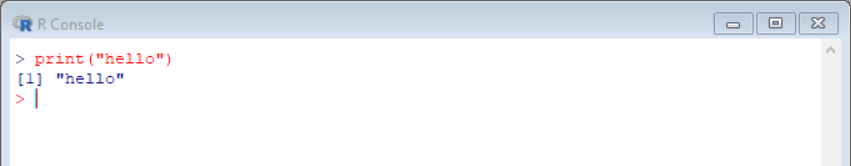
\includegraphics[width=0.85\textwidth]{figures/R-console-r}
  \caption[The R console]{The \Rpgrm console where the user can type textual commands one by one. Here the user has typed \code{print("Hello")} and \textit{entered} it by ending the line of text by pressing the ``enter'' key. The result of running the command is displayed below the command. The character at the head of the input line, a ``$>$'' in this case, is called the command prompt, signalling where a command can be typed in. Commands entered by the user are displayed in red, while results returned by R are displayed in blue.}\label{fig:intro:console}
\end{figure}

The \Rpgrm program does not have a graphical user interface (GUI), or menus from which to start different types of analyses. Instead, the user types the commands at the \Rpgrm console (Figure \ref{fig:intro:console}). The commands can be also saved into a text file, line by line, and such the file, called a `script' can substitute repeated typing of the same sequence of commands. When we work at the console typing in commands one by one, we say that we use R interactively. When we run script we may say that we run a ``batch job''.

The two approaches described above are part of the \Rpgrm program by itself. However, it is common to use a second program as a front-end or middle man ``in-between'' the user and the \Rpgrm program. Such a program allows more flexibility and has multiple features that makes entering commands or writing scripts easier---in other words makes it easier for the user to interact with \Rpgrm. Computations are still done by exactly the same \Rpgrm program. The simplest option is to use a text editor like \pgrmname{Emacs} to edit the scripts and then run the scripts in \Rpgrm from within the editor. With some editors like \pgrmname{Emacs}, rather good integration is possible. However, nowadays there are also Integrated Development Environments (IDEs) available for \Rpgrm. An IDE gives access to both use of the \Rpgrm console in a window, and provides a text editor for writing scripts in a separate window. Of the available IDEs for \Rpgrm, \RStudio is currently the most popular by a wide margin.

\subsubsection{Using R interactively}

A physical terminal (keyboard plus text-only screen) decades ago was how users communicated with computers, and was frequently called \emph{console}\index{console}. Nowadays, a text-only interface to a computer, in most cases a window or a pane within a graphical user interface it is still called a console. In our case, the \Rpgrm console (Figure \ref{fig:intro:console}). This is the native user interface of \Rpgrm.

Typing commands at the \Rpgrm console is useful when one is playing around, rather aimlessly exploring things, or trying to understand how an \Rpgrm function or operator we are not familiar with works. Once we want to keep track of what we are doing, there are better ways of using \Rpgrm, which allow us to keep a record of how an analysis has been carried out. The different ways of using \Rpgrm are not exclusive of each other, so most users will use the \Rpgrm console to test individual commands and plot data during the first stages of exploration. As soon as we decide how we want to plot or analyse the data, it is best to start using scripts. This is not enforced in any way by \Rpgrm, but scripts are what really brings to light the most important advantages of using a programming language for data analysis. In Figure \ref{fig:intro:console} we can see how the \Rpgrm console looks. The text in red has been typed in by the user---except for the prompt \code{$>$}---, and the text in blue is what \Rpgrm has displayed in response. It is essentially a dialogue between user and \Rpgrm. The console can \emph{look} different when displayed within an IDE like \RStudio, but the only difference is in the appearance of the text rather than in the text itself (cf.\ Figures \ref{fig:intro:console} and \ref{fig:intro:console:rstudio}).

\begin{figure}
  \centering
  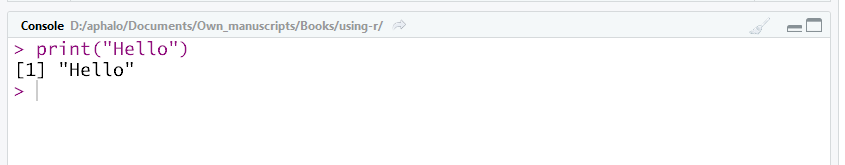
\includegraphics[width=\linewidth]{figures/r-console-rstudio}
  \caption[The R console]{The \Rpgrm console embedded in \RStudio. The same commands have been typed-in as in Figure \ref{fig:intro:console}. Commands entered by the user are displayed in purple, while results returned by \Rpgrm are displayed in black.}\label{fig:intro:console:rstudio}
\end{figure}

The two previous figures showed the result of entering a single command. Figure \ref{fig:intro:console:capture} shows how the console looks after the user has entered several commands, each as a separate line of text.

\begin{figure}
  \centering
  \includegraphics[width=\linewidth]{figures/r-console-capture}
  \caption[The R console]{The \Rpgrm console after several commands have been entered. Commands entered by the user are displayed in red, while results returned by \Rpgrm are displayed in blue.}\label{fig:intro:console:capture}
\end{figure}

The examples in this book require only the console window for user input. Menu-driven programs are not necessarily bad, they are just unsuitable when there is a need to set very many options and choose from many different actions. They are also difficult to maintain when extensibility is desired, and when independently developed modules of very different characteristics need to be integrated. Textual languages also have the advantage, to be dealt in later chapters, that command sequences can be stored in human- and computer readable text files. Such files constitute a record of all the steps used and in most cases makes it trivial to reproduce the same steps at a later time. Scripts are also a very simple and handy way of communicating to others how to do a given data analysis. When working at the command prompt, most results are printed by default, but in within scripts one needs to use the function \Rfunction{print()} explicitly.

\begin{explainbox}
In the console one types commands at the \code{>} prompt. When one ends a line by pressing the return or enter key, if the line can be interpreted as an R command, the result will be printed at the console, followed by a new \code{>} prompt.
If the command is incomplete a \code{+} continuation prompt will be shown, and you will be able to type-in the rest of the command. For example if the whole calculation that you would like to do is $1 + 2 + 3$, if you enter in the console \code{1 + 2 +} in one line, you will get a continuation prompt where you will be able to type \code{3}. However, if you type \code{1 + 2}, the result will be calculated, and printed.
\end{explainbox}

\subsubsection{Using R as a ``batch job''}

To run a script we need first to prepare a script in a text editor. Figure \ref{fig:intro:script} shows the console immediately after running the script file shown in the text editor. As before, red text, the command \code{source("my-script.R")}, was typed by the user, and the blue text in the console is what was displayed by \Rpgrm as a result of this action. The title bar of the console, shows ``R-console'', while the title bar of the editor shows the \emph{path} to the script file that is open and ready to be edited followed by ``R-editor''.

\begin{figure}
  \centering
  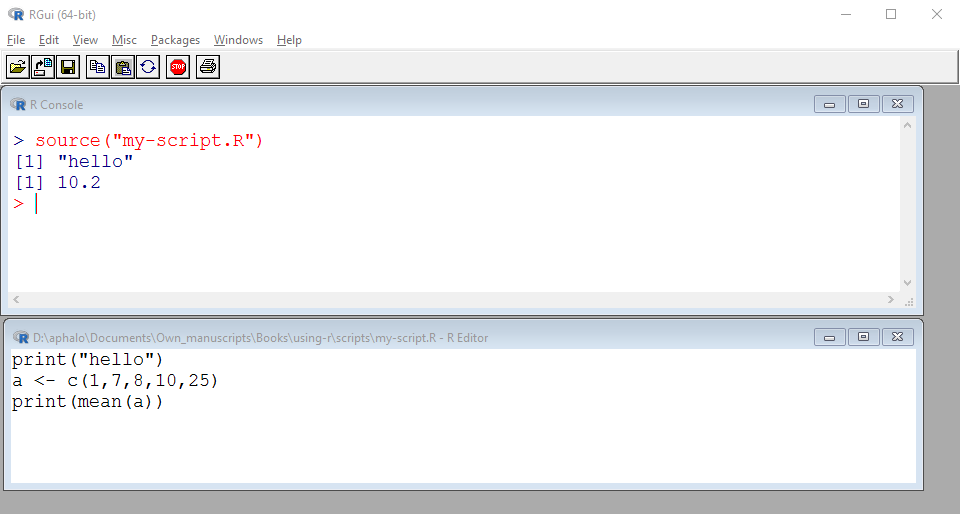
\includegraphics[width=\linewidth]{figures/R-console-script}
  \caption[Script sourced at the R console]{Screen capture of the \Rpgrm console and editor just after running a script. The upper pane shows the \Rpgrm console, and the lower pane the script file in an editor. }\label{fig:intro:script}
\end{figure}

A true ``batch job'' is not run at the \Rpgrm console but at the operating system command prompt, or shell. The shell is the console of the operating system---\osname{Linux}, \osname{Unix}, \osname{OS X}, or \osname{MS-Windows}. Figure \ref{fig:intro:shell} shows how running an script at the Windows command prompt looks. A script can be run at the operating system prompt to do time-consuming calculations with the output saved to a file. One may use this approach on a server, say, to leave a large data analysis job running over-night or for even several days.

\begin{figure}
  \centering
  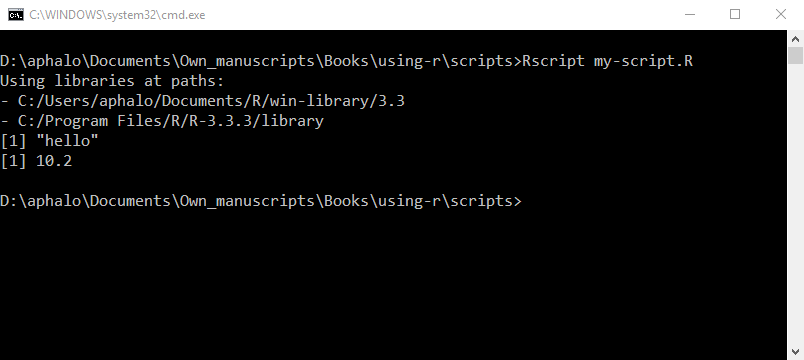
\includegraphics[width=\linewidth]{figures/windows-cmd-script}
  \caption[Script at the Windows cmd promt]{Screen capture of the \osname{MS-Windows} command console just after running the same script. Here we use \code{Rscript} to run the script, the exact syntax will depend on the operating system in use. In this case \Rpgrm prints the results at the operating system console or shell, rather than in its own \Rpgrm console.}\label{fig:intro:shell}
\end{figure}

Batch jobs are not the only, or main use of scripts, as they are useful even in data analysis jobs that take just seconds to run as they provide a way of keeping a faithful record of the steps that have been followed from data input to final analysis and graphical presentation.

\subsubsection{Editors and IDEs}

Integrated Development Environments (IDEs) are used when developing computer programs. IDEs provide a centralized user interface from within which the different tools used to create and test a computer program can be accessed and used in coordination. Most IDEs include a dedicated editor capable of syntax highlighting, and even report some mistakes, related to the programming language in use. One could describe such editor as the equivalent as a word processor with spelling and grammar checking, that can alert about spelling and syntax errors for a computer language like \Rlang instead of for a natural language like English. In the case of \RStudio, the main, but not only language supported is \Rlang. \RStudio in contrast to other IDEs targets also data analysis. The main window of IDEs usually displays more than one pane simultaneously. From within the \RStudio IDE one has access to the \Rpgrm console, a text editor, a file-system browser, a pane for graphical output, and access to several additional tools such the installation of extension packages. Although \RStudio supports very well the development of large scripts and packages, it is also the best possible way of using \Rpgrm at the console as it has the \Rpgrm help system very well integrated both in the editor and R console. Figure \ref{fig:intro:rstudio} shows the main window displayed by \RStudio after running the same script as shown above at the \Rpgrm console (Figure \ref{fig:intro:script}) and at the operating system command prompt (Figure \ref{fig:intro:shell}). We can see by comparing these three figures how \RStudio is really a layer between the user and an unmodified \Rpgrm executable. The script was sourced by pressing the ``Source'' button at the top of the editor pane. \RStudio in response to this generated the code needed to source the file and ``entered'' it at the console, the same console, where we would type ourselves any \Rpgrm commands.

\begin{figure}
  \centering
  \includegraphics[width=\linewidth]{figures/Rstudio-script}
  \caption[Script in Rstudio]{The \RStudio interface just after running the same script. Here we used the ``Source'' button to run the script. In this case \Rpgrm prints the results to the \Rpgrm console in the lower left pane.}\label{fig:intro:rstudio}
\end{figure}

When a script is run, if an error is triggered, \RStudio automatically finds the location of the error. \RStudio also supports the concept of projects allowing saving of settings per project. Some features are beyond what you need for everyday data analysis and aimed at package development, such as integration of debugging, traceback on errors, profiling and bench marking of code so as to analyse and improve performance. It also integrates support for file version control, which is not only useful for package development, but also for keeping track of the progress or collaboration in the analysis of data.

The version of \RStudio that one uses locally, i.e.\ installed in a computer used locally by a single user, runs with almost identical user interface on most modern operating systems, such as \osname{Linux}, \osname{Unix}, \osname{OS X}, and \osname{MS-Windows}. There is also a server version that runs on \osname{Linux}, and that can be used remotely through a web browser. The user interface is still the same.

\RStudio is under active development, and constantly improved. Visit \url{http://www.rstudio.org/} for an up-to-date description and download and installation instructions. Two books \autocite{vanderLoo2012,Hillebrand2015} describe and teach how to use \RStudio without going in depth into data analysis or statistics, however, as \RStudio is under very active development several recently added important features are not described in these books. You will find tutorials and up-to-date cheat sheets at \url{http://www.rstudio.org/}.

\section{Packages and repositories}
\index{packages!extending R}
The most elegant way of adding new features or capabilities to \Rlang is through packages. This is without doubt the best mechanism when these extensions to \Rlang need to be shared. However, in most situations it is also the best mechanism for managing code that will be reused even by a single person over time. \Rlang packages have strict rules about their contents, file structure, and documentation, which makes it possible among other things for the package documentation to be merged into \Rpgrm's help system when a package is loaded. With a few exceptions, packages can be written so that they will work on any computer where \Rpgrm runs.

Packages can be shared as source or binary package files, sent for example through e-mail. However, for sharing packages widely, best is to submit them to a repository. The largest public repository of \Rpgrm packages is called CRAN\index{CRAN}, an acronym for Comprehensive R Archive Network. Packages available through CRAN are guaranteed to work, in the sense of not failing any tests built into the package and not crashing or aborting prematurely. They are tested daily, as they may depend on other packages whose code will change when updated. In January 2017, the number of packages available through CRAN passed the 10\,000 mark.

Using packages requires in general two steps: 1) installing the package into the \Rpgrm library\index{packages!library}\index{packages!installation} and 2) loading it from the library into the current \Rpgrm session\index{packages!loading}. Installation is needed once and consists in making a local copy of the package, i.e.\ in the hard disk. Loading needs to be done at least once in each \Rpgrm session, and before any command defined in the package can be used. Loading a package also loads the corresponding help pages.

Packages are installed into the library using function \Rfunction{install.packages()} and are loaded from the library with function \Rfunction{library()}.

\begin{playground}
  Use \code{help} to look up the help pages for \code{install.packages} and \code{library}, and explain what the code in the next chunk does.
\begin{knitrout}\footnotesize
\definecolor{shadecolor}{rgb}{0.969, 0.969, 0.969}\color{fgcolor}\begin{kframe}
\begin{alltt}
\hlkwd{install.packages}\hlstd{(learnrbook)}
\hlkwd{library}\hlstd{(learnrbook)}
\hlkwd{help}\hlstd{(learnrbook)}
\end{alltt}
\end{kframe}
\end{knitrout}
\end{playground}

When using an IDE like \RStudio, although these commands can be typed into the \Rpgrm console, it is usually easier to manage installation and update of packages through the IDE's interface, which in turn generates the needed \Rlang code and runs it in the console.

Loading of packages seems to me easier directly at the console or as part of a script. Of course, this is my own preference that may differ from yours!

\section{Reproducible data analysis}
\index{reproducible data analysis|(}
Reproducible data analysis is much more than a fashionable buzzword. Under any situation where accountability is important, from scientific research to decision making in commercial enterprises, industrial quality control and safety and environmental impact assessments, being able to reproduce a data analysis reaching the same conclusions from the same data is crucial. Most approaches to reproducible data analysis are based on automating report generation and including as part of the report all the computer commands used to generate the results presented.

A fundamental requirement for reproducibility, is a reliable record of what commands have been run on which data. Such a record is specially difficult to keep when issuing commands through menus and dialogue boxes in a graphical user interface or interactively at a console. Even working interactively at the \Rpgrm console using copy and paste to include commands and results in a report is error prone, and laborious.

A further requirement is to be able to match the output of the \Rlang commands to the input. If the script saves the output to separate files, then the user will need to take care that the script saved or shared as record of the data analysis was the one actually used for obtaining the reported results and conclusions. This is another error prone stage in the reporting of a data analysis. To solve this problem an approach was developed, inspired in what is called \emph{literate programming} \autocite{Knuth1984a}. The idea is that running the script will produce a document that includes the script, the results of running the scripts and any explanatory text needed to understand and interpret the analysis.

Although a system capable of producing such reports with \Rlang, called \pkgname{Sweave} \autocite{Leisch2002}, has been available for a couple decades, it was rather limited and not supported by an IDE, making its use rather tedious. A more recently developed system called \pkgname{knitr} \autocite{Xie2013} together with its integration into \RStudio has made the use of this type of reports very easy. The most recent development is what has been called \Rlang \emph{notebooks} produced within \RStudio. This new feature, can produce the readable report of running the script as an HTML file, displaying the code used interspersed with the results within the viewable file as in earlier approaches. However, this newer approach goes even further: the actual source script used to generate the report is embedded in the HTML file of the report and can be extracted and run very easily and consequently re-used. This means that anyone who gets access to the output of the analysis in human readable form also gets access to the code used to generate the report, in computer executable format.

Because of these recent developments, \Rlang is an ideal language to use when the goal of reproducibility is important. During recent years the problem of the lack of reproducibility in scientific research has been broadly discussed and analysed \autocite{Gandrud2015}. One of the problems faced when attempting to reproduce experimental work, is reproducing the data analysis. \Rlang together with these modern tools can help in avoiding this source of lack of reproducibility.

How powerful are these tools? and how flexible? They are powerful and flexible enough to write whole books, such as this very book you are now reading, produced with \Rpgrm, \pkgname{knitr} and \LaTeX\index{Latex@\LaTeX}. All pages in the book are generated directly, all figures are generated by \Rpgrm and included automatically, except for the figures in this chapter that have been manually captured from the computer screen. Why am I using this approach? First because I want to make sure that every bit of code as you will see printed, runs without error. In addition I want to make sure that the output that you will see below every line or chunk of \Rlang language code is exactly what \Rpgrm returns. Furthermore, it saves a lot of work for me as author, as I can just update \Rpgrm and all the packages used to their latest version, and build the book again, to keep it up to date and free of errors.

Although the use of these tools is important, they are outside the scope of this book and well described in other books \autocite{Gandrud2015,Xie2013}. Still when writing code, using a consistent style for formatting and indentation, carefully choosing variable names, and adding textual explanations in comments when needed, helps very much with readability for humans. I have tried to be as consistent as possible throughout the whole book in this respect, with only small personal deviations from the usual style.
\index{reproducible data analysis|)}

\section{Finding additional information}

When searching for answers, asking for advice or reading books you will be confronted with different ways of approaching the same tasks. Do not allow this to overwhelm you, in most cases it will not matter as many computations can be done in \Rpgrm, as in any language, in several different ways, still obtaining the same result. The different approaches may differ mainly in two aspects: 1) how readable to humans are the instructions given to the computer as part of a script or program, and 2) how fast the code runs. Unless computation time is an important bottleneck in your work, just concentrate on writing code that is easy to understand to you and to others, and consequently easy to check and reuse. Of course do always check any code you write for mistakes, preferably using actual numerical test cases for any complex calculation or even relatively simple scripts. Testing and validation are extremely important steps in data analysis, so get into this habit while reading this book. Testing how every function works as I will challenge you to do in this book, is at the core of any robust data analysis or computing programming.

\begin{warningbox}
Error messages tend to be terse in \Rpgrm, and may require some lateral thinking and/or `experimentation' to understand the real cause behind problems. When you are not sure to understand how some command works, it is useful in many cases to try simple examples for which you know the correct answer and see if you can reproduce them with \Rpgrm. Because of this, this book also includes some code examples that trigger errors. Learning to interpret error messages is part of what is needed to become a proficient user of \Rlang. To test your understanding of how a code statement or function works, it is good to try your hand at testing its limits, testing which variations of a piece code are valid or not.
\end{warningbox}

\subsection{R's built-in help}

To\index{R!help} access help pages through the command prompt we use function \Rfunction{help()} or a question mark. Every object exported by an \Rlang package (functions, methods, classes, data) is documented. Sometimes a single help page documents several \Rlang objects. Usually at the end of the help pages, some examples are given, which tend to help very much in learning how to use the functions described. For example one can search for a help page at the \Rpgrm console.

\begin{knitrout}\footnotesize
\definecolor{shadecolor}{rgb}{0.969, 0.969, 0.969}\color{fgcolor}\begin{kframe}
\begin{alltt}
\hlkwd{help}\hlstd{(}\hlstr{"sum"}\hlstd{)}
\hlopt{?}\hlstd{sum}
\end{alltt}
\end{kframe}
\end{knitrout}

\begin{playground}
Look at help for some other functions like \code{mean()}, \code{var()}, \code{plot()} and, why not, \Rfunction{help()} itself!
\begin{knitrout}\footnotesize
\definecolor{shadecolor}{rgb}{0.969, 0.969, 0.969}\color{fgcolor}\begin{kframe}
\begin{alltt}
\hlkwd{help}\hlstd{(help)}
\end{alltt}
\end{kframe}
\end{knitrout}
\end{playground}

When using \RStudio there are easier ways of navigating to a help page than using function \Rfunction{help()}, for example with the cursor on the name of a function in the editor or console, pressing the F1 key, opens the corresponding help page in the help pane. Letting the cursor hover for a few seconds over the name of a function at the \Rpgrm console will open ``bubble help'' for it. If the function is defined in a script or another file open in the editor pane one can directly navigate from the line where the function is called to where it is defined. In \RStudio one can also search for help through the graphical interface.

In addition to help pages, the \Rpgrm's distribution includes useful manuals as PDF or HTML files. These can be accessed most easily through the Help menu in \RStudio or \pgrmname{RGUI}. Extension packages, provide help pages for the functions and data they export. When a package is loaded into an \Rpgrm session, its help pages are added to the native help of \Rpgrm. In addition to these individual help pages, each package, provides an index of its corresponding help pages, for users to browse. Many packages, also provide \emph{vignettes} such as User Guides or articles describing the algorithms used.

There are some web sites that give access to \Rlang documentation through a web server. These sites can be very convenient when exploring whether a certain package could be useful for a certain problem, as they allow browsing and searching the documentation without need of installing the packages. Some package maintainers have web sites with additional documentation for their own packages. The DESCRIPTION or README of packages provide contact information for the maintainer, links to web sites, and instructions on how to report bugs. As packages are contributed by independent authors, they should be cited in addition to citing \Rpgrm itself. \Rlang function \code{citation()} with the name of a package as argument provides the reference that should be cited, and without an explicit argument, the reference to use for the version of \Rlang in use.

\begin{knitrout}\footnotesize
\definecolor{shadecolor}{rgb}{0.969, 0.969, 0.969}\color{fgcolor}\begin{kframe}
\begin{alltt}
\hlkwd{citation}\hlstd{()}
\end{alltt}
\begin{verbatim}
## 
## To cite R in publications use:
## 
##   R Core Team (2018). R: A language and environment for
##   statistical computing. R Foundation for Statistical Computing,
##   Vienna, Austria. URL https://www.R-project.org/.
## 
## A BibTeX entry for LaTeX users is
## 
##   @Manual{,
##     title = {R: A Language and Environment for Statistical Computing},
##     author = {{R Core Team}},
##     organization = {R Foundation for Statistical Computing},
##     address = {Vienna, Austria},
##     year = {2018},
##     url = {https://www.R-project.org/},
##   }
## 
## We have invested a lot of time and effort in creating R, please
## cite it when using it for data analysis. See also
## 'citation("pkgname")' for citing R packages.
\end{verbatim}
\end{kframe}
\end{knitrout}

\begin{playground}
  Look at the help page for function \code{citation()} for a discussion of why it is important for users to cite \Rpgrm and packages when using them.
\end{playground}

\subsection{Obtaining help from on-line forums}

When consulting help pages, vignettes and possibly books at hand fails to provide the information the next step to follow is to search internet forums for existing answers to one's questions. When these steps fail to solve a problem, then it is time to ask for help, either from local experts or by posting your own question in a suitable on-line forum. When posting requests for help one needs to abide to what is usually described as ``netiquette''.

\subsubsection{Netiquette}
In\index{netiquette}\index{network etiquette} most internet forums, a certain behaviour is expected from those asking and answering questions. Some types of miss-behavior, like use of offensive or inappropriate language, will usually result in the user losing writing rights in a forum. Occasional minor miss-behaviour, will usually result in the original question not being answered and instead the problem highlighted in the reply. In general following the steps listed below will greatly increase your chances of getting a detailed and useful answer.

\begin{itemize}
  \item Do your homework: first search for existing answers to your question, both on-line and in the documentation. (Do mention that you attempted this without success when you post your question.)
  \item Provide a clear explanation of the problem, and all the relevant information. Say if it concerns \Rpgrm, the version, operating system, and any packages loaded and their versions.
  \item If at all possible provide a simplified and short, but self-contained, code example that reproduces the problem (sometimes called \emph{reprex}).
  \item Be polite.
  \item Contribute to the forum by answering other users' questions when you know the answer.
\end{itemize}

\subsubsection{StackOverflow}

Nowadays, StackOverflow (\url{http://stackoverflow.com/})\index{StackOverflow} is the best questions and answers (Q\,\&\,A) support site for \Rpgrm. In most cases, searching for existing questions and their answers, will be all what you need to do. If asking a question, make sure that it is really a new question. If there is some question that looks similar, make clear how your question is different.

StackOverflow has a user-rights system based on reputation, and questions and answers can be up- and down-voted. Those with the most up-votes are listed at the top of searches. If the questions or answers you write are up-voted after you accumulate enough reputation you acquire badges, and rights, such as editing other users' questions and answers or later on, even deleting wrong answers or off-topic questions from the system. This sounds complicated, but works extremely well at ensuring that the base of questions and answers is relevant and correct, without relying on a single or ad-hoc \emph{moderators}.

\subsubsection{Reporting bugs}

Being careful in the preparation of a reproducible example\index{reproducible example}\index{reprex|see{reproducible example}} is specially important when you intend to report a bug to the maintainer of any piece of software. For the problem to be fixed, the person revising the code, needs to be able to reproduce the problem, and after modifying the code, needs to be able to test if the problem has been solved or not. However, even if you are facing a problem caused by your misunderstanding of how \Rlang works, the simpler the example, the more likely that someone will quickly realize what was your intention when writing the code that produces a result different from what you expected.

\begin{explainbox}
How to prepare a reproducible example\index{reproducible example} (``reprex''). A \emph{reprex} is a self-contained and as simple as possible piece of computer code that triggers (and so demonstrates) a problem. If possible when you need to use data, either use a data set included in base \Rpgrm or generate artificial data within the reprex code. If you can reproduce the problem only with your own data, then you need to provide a minimal subset of it that triggers the problem.

While preparing the \emph{reprex} you will need to simplify the code, and sometimes this already makes a diagnose by yourself much likely. In general, before, posting a reprex on-line, it is wise to check it with the latest versions of \Rpgrm and any package being used.

I would say that about two out of three times I start preparing a \emph{reprex}, preparing the \emph{reprex} allows me to much better understand the problem and find the root of the problem or a work-around on my own.
\end{explainbox}

\section{What is needed to run the examples in this book?}

The book is written with the expectation that you will run most of the code examples and try as many other variations as needed until you are sure to understand the basic `rules' of the \Rpgrm language and how each function or command described works. As mentioned above, you are expected to use this book as a travel guide for your exploration of the world of \Rlang.

\Rpgrm is all what is needed to work through all the examples in this book, but it is not a convenient way of doing this. I recommend you to use an editor or an IDE, in particular \RStudio\index{IDE for R}\index{editor for R scripts}. \RStudio is user friendly, actively maintained, free, open-source and available both in desktop and server versions. The desktop version runs on \osname{MS-Windows}, \osname{Linux}, and \osname{OS X} and other \osname{Unix} distributions.

Of course when choosing which editor to use, personal preferences and previous familiarity play an important role.
Currently, for the development of packages, I use \RStudio exclusively. For writing this book I have used both \RStudio and the text editor \pgrmname{WinEdt} which also has support for \Rpgrm together with excellent support for \LaTeX\index{Latex@\LaTeX}. When working on a large project or collaborating with other data analysts or researchers, one big advantage of a system based on plain text files such as R scripts, is that the same files can be edited with different programs and under different operating systems as needed or wished by the different persons involved in a project.

When I started using \Rpgrm, nearly two decades ago, I was using other editors, using the operating system shell a lot more, and struggling with debugging as no IDE was available. The only reasonably good integration with an editor was for \pgrmname{Emacs}, which was widely available only under \osname{Unix}-like systems. Given my past experience, I encourage you to use an IDE for \Rpgrm. \RStudio is nowadays very popular, but if you do not like it, need a different set of features, such as integration with \pgrmname{ImageJ}, or are already familiar with the \pgrmname{Eclipse} IDE, you may want to try the \pgrmname{Bio7} IDE, available from \url{http://bio7.org}.

The examples in this book make use of several freely available packages, which can be installed from CRAN. One of them \pkgname{learnrbook} also available through CRAN, contains data sets and files specific to this book. The \pkgname{learnrbook} package also contains installation instructions and saved lists of the names of all other packages used in the book. Instructions on installing \Rpgrm, \pgrmname{Git}, \RStudio, compilers and other tools are available on-line. In many cases the IT staff at your employer or school will know how to install them, or they may be even included in the default computer setup. In addition a web site supporting the book will be available at: \url{http://www.learnr-book.info}.





% !Rnw root = appendix.main.Rnw



\chapter{The R language: ``words'' and ``sentences''}\label{chap:R:as:calc}

\begin{VF}
The desire to economize time and mental effort in arithmetical computations, and to eliminate human liability to error, is probably as old as the science of arithmetic itself.

\VA{Howard Aiken}{Proposed automatic calculating machine}
\end{VF}

%\dictum[Howard Aiken, \emph{Proposed automatic calculating machine}, presented to IBM in 1937]{The desire to economize time and mental effort in arithmetical computations, and to eliminate human liability to error, is probably as old as the science of arithmetic itself.}\vskip2ex

\section{Aims of this chapter}

In my experience, for those not familiar with computer programming languages, the best first step in learning the \Rlang language is to use it interactively by issuing textual commands at the \emph{console}. This will teach not only the syntax and grammar rules, but also give a glimpse at the advantages and flexibility of this approach to data analysis.

In the first part of the chapter we will use \Rlang to do everyday calculations that should be so easy and familiar that you will not need to think about the operations themselves. This easy start will give you a chance to focus on learning how to issue textual commands at the command prompt.

Later in the chapter, you will gradually need to focus more on the \Rlang language and its grammar and less on how commands are entered. By the end of the chapter you will be familiar with most of the kinds of ``words'' used in the \Rlang language and you will be able to write simple ``sentences'' in \Rlang.

Along the chapter, I will show occasionally the equivalent of the \Rlang code in mathematical notation. If you are not familiar with the mathematical notation, you can safely ignore it, as long as you understand the \Rlang code.

\section{Natural and computer languages}
\index{languages!natural and computer}
Computer languages have strict rules and interpreters and compilers are unforgiving about errors. They will issue error messages, but in contrast to human readers or listeners, will not guess your intentions and continue. However, computer languages have a much smaller set of words than natural languages, such as English. If you are new to computer programming, understanding the parallels between computer and natural languages may be useful.

One can think of constant values and variables (values stored under a name) as nouns and of operators and functions as verbs. A complete command, or statement, is the equivalent of a natural language sentence: ``a comprehensible utterance''. The simple statement \code{a + 1} has three components: \code{a}, a variable, \code{+}, an operator and \code{1} a constant. The statement \code{sqrt(4)} has two components, a function \code{sqrt()} and a numerical constant \code{4}. We say that ``to compute $\sqrt{4}$ we \emph{call} \code{sqrt()} with \code{4} as its \emph{argument}''.

In later chapters you will learn how to write compound statements, the equivalent of natural-language paragraphs, and scripts, the equivalent of essays. You will also learn how to define new verbs, user defined functions and operators, and new nouns, user defined classes.

\section{Numeric values and arithmetic}
\index{classes and modes!numeric, integer, double|(}\index{numbers and their arithmetic|(}\qRclass{numeric}\index{math operators}\index{math functions}\index{numeric values}\qRoperator{+}\qRoperator{-}\qRoperator{*}\qRoperator{/}
When working in \Rlang with arithmetic expressions, the normal mathematical precedence rules are respected, but parentheses can be used to alter this order. Parentheses can be nested, but in contrast to the usual practice in mathematics, the same parenthesis symbol is used at all nesting levels. It must also be remembered that trigonometric \Rlang functions interpret numeric values representing angles passed as arguments as being expressed in radians.

The equivalent of the math expression\qRfunction{exp()}\qRfunction{sin()}\qRconst{pi}
$$
\frac{3 + e^2}{\sin \pi}
$$
is
\begin{knitrout}\footnotesize
\definecolor{shadecolor}{rgb}{0.969, 0.969, 0.969}\color{fgcolor}\begin{kframe}
\begin{alltt}
\hlstd{(}\hlnum{3} \hlopt{+} \hlkwd{exp}\hlstd{(}\hlnum{2}\hlstd{))} \hlopt{/} \hlkwd{sin}\hlstd{(pi)}
\end{alltt}
\begin{verbatim}
## [1] 8.483588e+16
\end{verbatim}
\end{kframe}
\end{knitrout}

It can be seen above that mathematical constants and functions are part of the \Rlang language. One thing to remember when translating complex fractions as above into \Rlang code, is that in arithmetic expressions the bar of the fraction generates a grouping that alters the normal precedence of operations. In contrast, in an \Rlang expression the grouping must be explicitly signaled with additional parentheses.

If you are in doubt about how precedence rules work, you can add parentheses to make sure the order of computations is the one you intend. Redundant parentheses have no effect.

\begin{knitrout}\footnotesize
\definecolor{shadecolor}{rgb}{0.969, 0.969, 0.969}\color{fgcolor}\begin{kframe}
\begin{alltt}
\hlnum{1} \hlopt{+} \hlnum{2} \hlopt{*} \hlnum{3}
\end{alltt}
\begin{verbatim}
## [1] 7
\end{verbatim}
\begin{alltt}
\hlnum{1} \hlopt{+} \hlstd{(}\hlnum{2} \hlopt{*} \hlnum{3}\hlstd{)}
\end{alltt}
\begin{verbatim}
## [1] 7
\end{verbatim}
\begin{alltt}
\hlstd{(}\hlnum{1} \hlopt{+} \hlnum{2}\hlstd{)} \hlopt{*} \hlnum{3}
\end{alltt}
\begin{verbatim}
## [1] 9
\end{verbatim}
\end{kframe}
\end{knitrout}

The number of opening (left side) and closing (right side) parentheses must be balanced, and they must be located so that each enclosed term is a valid mathematical expression. For example while \code{(1 + 2) * 3} is valid, \code{(1 +) 2 * 3} is a syntax error as \code{1 +} is incomplete and cannot be calculated.

\begin{playground}
Here results are not shown. These are examples for you to type at the command prompt. In general you should not skip them, as in many cases, as with the statements highlighted with comments in the code chunk below, they have something to teach or demonstrate. You are also strongly encouraged to \emph{play}, in other words, create new variations of the examples and execute them to explore how \Rlang works.\qRfunction{sqrtt()}\qRfunction{sin()}\qRfunction{log(), log10(), log2()}\qRfunction{exp()}

\begin{knitrout}\footnotesize
\definecolor{shadecolor}{rgb}{0.969, 0.969, 0.969}\color{fgcolor}\begin{kframe}
\begin{alltt}
\hlnum{1} \hlopt{+} \hlnum{1}
\hlnum{2} \hlopt{*} \hlnum{2}
\hlnum{2} \hlopt{+} \hlnum{10} \hlopt{/} \hlnum{5}
\hlstd{(}\hlnum{2} \hlopt{+} \hlnum{10}\hlstd{)} \hlopt{/} \hlnum{5}
\hlnum{10}\hlopt{^}\hlnum{2} \hlopt{+} \hlnum{1}
\hlkwd{sqrt}\hlstd{(}\hlnum{9}\hlstd{)}
\hlstd{pi} \hlcom{# whole precision not shown when printing}
\hlkwd{print}\hlstd{(pi,} \hlkwc{digits} \hlstd{=} \hlnum{22}\hlstd{)}
\hlkwd{sin}\hlstd{(pi)} \hlcom{# oops! Read on for explanation.}
\hlkwd{log}\hlstd{(}\hlnum{100}\hlstd{)}
\hlkwd{log10}\hlstd{(}\hlnum{100}\hlstd{)}
\hlkwd{log2}\hlstd{(}\hlnum{8}\hlstd{)}
\hlkwd{exp}\hlstd{(}\hlnum{1}\hlstd{)}
\end{alltt}
\end{kframe}
\end{knitrout}

\end{playground}

Variables\index{variables}\index{assignment} are used to store values. After we \emph{assign} a value to variable, we can use the name of the variable in place of the stored value. The `usual' assignment operator is \Roperator{<-}. In \Rlang all names, including variable names, are case sensitive. Variables \code{a} and \code{A} are two different variables. Variable names can be quite long, but usually it is not a good idea to use very long names. Here I am using very short names, something that is usually also a very bad idea. However, in the examples in this chapter where the stored values have no connection to the real world, simple names emphasize their abstract nature.

\begin{knitrout}\footnotesize
\definecolor{shadecolor}{rgb}{0.969, 0.969, 0.969}\color{fgcolor}\begin{kframe}
\begin{alltt}
\hlstd{a} \hlkwb{<-} \hlnum{1}
\hlstd{a} \hlopt{+} \hlnum{1}
\end{alltt}
\begin{verbatim}
## [1] 2
\end{verbatim}
\begin{alltt}
\hlstd{a}
\end{alltt}
\begin{verbatim}
## [1] 1
\end{verbatim}
\begin{alltt}
\hlstd{b} \hlkwb{<-} \hlnum{10}
\hlstd{b} \hlkwb{<-} \hlstd{a} \hlopt{+} \hlstd{b}
\hlstd{b}
\end{alltt}
\begin{verbatim}
## [1] 11
\end{verbatim}
\begin{alltt}
\hlnum{3e-2} \hlopt{*} \hlnum{2.0}
\end{alltt}
\begin{verbatim}
## [1] 0.06
\end{verbatim}
\end{kframe}
\end{knitrout}

Entering the name of a variable \emph{at the R console} implicitly calls function \code{print()} displaying the stored value on the console. Unless assigned to a variable, the result of entering a statement \emph{at the R console} is displayed on the console as \code{print()} is implicitly called with the result of the statement as its argument.

\begin{knitrout}\footnotesize
\definecolor{shadecolor}{rgb}{0.969, 0.969, 0.969}\color{fgcolor}\begin{kframe}
\begin{alltt}
\hlstd{a}
\end{alltt}
\begin{verbatim}
## [1] 1
\end{verbatim}
\begin{alltt}
\hlkwd{print}\hlstd{(a)}
\end{alltt}
\begin{verbatim}
## [1] 1
\end{verbatim}
\begin{alltt}
\hlstd{a} \hlopt{+}\hlnum{1}
\end{alltt}
\begin{verbatim}
## [1] 2
\end{verbatim}
\begin{alltt}
\hlkwd{print}\hlstd{(a} \hlopt{+}\hlnum{1}\hlstd{)}
\end{alltt}
\begin{verbatim}
## [1] 2
\end{verbatim}
\end{kframe}
\end{knitrout}
\begin{playground}
There are some syntactically legal statements that are not very frequently used, but you should be aware that they are valid, as they will not trigger error messages, and may surprise you. The most important thing is to write code consistently. The `backwards' assignment operator \Roperator{->} and resulting code like \code{1 -> a}\index{assignment!leftwise} are valid but less frequently used. The use of the equals sign (\Roperator{=}) for assignment in place of \Roperator{<-} although valid is generally discouraged as this redundant use was not part of the \Rlang language as originally defined. Chaining\index{assignment!chaining} assignments as in the first line below is sometimes used, and signals to the human reader that \code{a}, \code{b} and \code{c} are being assigned the same value.

\begin{knitrout}\footnotesize
\definecolor{shadecolor}{rgb}{0.969, 0.969, 0.969}\color{fgcolor}\begin{kframe}
\begin{alltt}
\hlstd{a} \hlkwb{<-} \hlstd{b} \hlkwb{<-} \hlstd{c} \hlkwb{<-} \hlnum{0.0}
\hlstd{a}
\hlstd{b}
\hlstd{c}
\hlnum{1} \hlkwb{->} \hlstd{a}
\hlstd{a}
\hlstd{a} \hlkwb{=} \hlnum{3}
\hlstd{a}
\end{alltt}
\end{kframe}
\end{knitrout}

\end{playground}

\begin{explainbox}
Here\index{mode of an object} I very briefly introduce the concept of \emph{mode} of an \Rlang object. In the case of \Rlang, numbers, belong to mode \Rclass{numeric}. We can query if the mode of an object is \Rclass{numeric} with function \Rfunction{is.numeric()}.

\begin{knitrout}\footnotesize
\definecolor{shadecolor}{rgb}{0.969, 0.969, 0.969}\color{fgcolor}\begin{kframe}
\begin{alltt}
\hlkwd{mode}\hlstd{(}\hlnum{1}\hlstd{)}
\end{alltt}
\begin{verbatim}
## [1] "numeric"
\end{verbatim}
\begin{alltt}
\hlstd{a} \hlkwb{<-} \hlnum{1}
\hlkwd{mode}\hlstd{(a)}
\end{alltt}
\begin{verbatim}
## [1] "numeric"
\end{verbatim}
\begin{alltt}
\hlkwd{is.numeric}\hlstd{(a)}
\end{alltt}
\begin{verbatim}
## [1] TRUE
\end{verbatim}
\end{kframe}
\end{knitrout}

One can think informally of a \emph{mode}, as a ``type'' or ``kind'' of objects. Constants like \code{1} or variables such as \code{a} in the code chunk above, belong to, or have a mode, that indicates that they are numbers. Other modes that we will use later in the present chapter are \Rclass{logical} and \Rclass{character} (We will discuss the concepts of \emph{mode} and \emph{class}, as used in \Rlang, in section \ref{sec:rlang:mode} on page \pageref{sec:rlang:mode}).

As in computers numbers can be stored in different formats requiring different amounts of memory, most computing languages implement several different types of numbers. In most cases \Rpgrm's \Rfunction{numeric()} can be used everywhere where a number is expected. In some cases it can be more efficient to explicitly indicate whether we will store or operate on integer numbers, in which case we can use class \Rclass{integer}, with integer constants indicated with a trailing capital `L', as in  \code{32L}.

Real numbers are a mathematical abstraction, and do not have an exact equivalent in computers. Instead of Real numbers, computers store and operate on numbers that are restricted to a broad but finite range values and have a finite resolution. They are called, \emph{floats} (or \emph{floating-point} numbers), in \Rlang they go by the name of \Rclass{double} and can be created with the constructor \Rfunction{double()}.

\begin{knitrout}\footnotesize
\definecolor{shadecolor}{rgb}{0.969, 0.969, 0.969}\color{fgcolor}\begin{kframe}
\begin{alltt}
\hlkwd{is.numeric}\hlstd{(}\hlnum{1L}\hlstd{)}
\end{alltt}
\begin{verbatim}
## [1] TRUE
\end{verbatim}
\begin{alltt}
\hlkwd{is.integer}\hlstd{(}\hlnum{1L}\hlstd{)}
\end{alltt}
\begin{verbatim}
## [1] TRUE
\end{verbatim}
\begin{alltt}
\hlkwd{is.double}\hlstd{(}\hlnum{1L}\hlstd{)}
\end{alltt}
\begin{verbatim}
## [1] FALSE
\end{verbatim}
\end{kframe}
\end{knitrout}

The name \code{double} originates from the \Clang language, in which there are different types of floats available. With the name \code{double} used to mean ``double-precision floating-point numbers''. Similarly, the use of \code{L} stems the \texttt{long} type in \Clang, meaning ``long integer numbers''.
\end{explainbox}

Numeric variables can contain more than one value. Even single numbers are in \Rlang \Rclass{vector}s of length one. We will later see why this is important. As you have seen above, the results of calculations were printed preceded with \code{[1]}. This is the index or position in the vector of the first number (or other value) displayed at the head of the current line.

One can use \Rmethod{c()} `concatenate' to create a vector from other vectors, including vectors of length 1, such as the \code{numeric} constants in the statements below.

\begin{knitrout}\footnotesize
\definecolor{shadecolor}{rgb}{0.969, 0.969, 0.969}\color{fgcolor}\begin{kframe}
\begin{alltt}
\hlstd{a} \hlkwb{<-} \hlkwd{c}\hlstd{(}\hlnum{3}\hlstd{,} \hlnum{1}\hlstd{,} \hlnum{2}\hlstd{)}
\hlstd{a}
\end{alltt}
\begin{verbatim}
## [1] 3 1 2
\end{verbatim}
\begin{alltt}
\hlstd{b} \hlkwb{<-} \hlkwd{c}\hlstd{(}\hlnum{4}\hlstd{,} \hlnum{5}\hlstd{,} \hlnum{0}\hlstd{)}
\hlstd{b}
\end{alltt}
\begin{verbatim}
## [1] 4 5 0
\end{verbatim}
\begin{alltt}
\hlstd{c} \hlkwb{<-} \hlkwd{c}\hlstd{(a, b)}
\hlstd{c}
\end{alltt}
\begin{verbatim}
## [1] 3 1 2 4 5 0
\end{verbatim}
\begin{alltt}
\hlstd{d} \hlkwb{<-} \hlkwd{c}\hlstd{(b, a)}
\hlstd{d}
\end{alltt}
\begin{verbatim}
## [1] 4 5 0 3 1 2
\end{verbatim}
\end{kframe}
\end{knitrout}

Method \code{c()} accepts as argument two or more vectors and concatenates them, one after another. Quite frequently we may need to insert one vector in the middle of another. For this operation, \code{c()} is not useful by itself. One could use indexing combined with \code{c()}, but this is not needed as R provides a function capable of directly doing this operation. Although it can be used to ``insert'' values it is named \code{append()}, and by default, it indeed appends one vector at the end of another.

\begin{knitrout}\footnotesize
\definecolor{shadecolor}{rgb}{0.969, 0.969, 0.969}\color{fgcolor}\begin{kframe}
\begin{alltt}
\hlkwd{append}\hlstd{(a, b)}
\end{alltt}
\begin{verbatim}
## [1] 3 1 2 4 5 0
\end{verbatim}
\end{kframe}
\end{knitrout}

The output above is the same as for \code{c(a, b)}, however, \Rfunction{append()} accepts as argument an index position after which to ``append'' its second argument. This results in an \emph{insert} operation when the index points at any position different from the end of the vector.

\begin{knitrout}\footnotesize
\definecolor{shadecolor}{rgb}{0.969, 0.969, 0.969}\color{fgcolor}\begin{kframe}
\begin{alltt}
\hlkwd{append}\hlstd{(a,} \hlkwc{values} \hlstd{= b,} \hlkwc{after} \hlstd{=} \hlnum{2L}\hlstd{)}
\end{alltt}
\begin{verbatim}
## [1] 3 1 4 5 0 2
\end{verbatim}
\end{kframe}
\end{knitrout}

Both \code{c()} and \code{append()} can be also used with lists.

\begin{playground}
One can create sequences\index{sequence} using function \Rfunction{seq()} or the operator \Roperator{:}, or repeat values using function \Rfunction{rep()}. In this case I leave to the reader to work out the rules by running these and his/her own examples, with the help of the documentation, available through \code{help(seq)} and \code{help(rep)}.

\begin{knitrout}\footnotesize
\definecolor{shadecolor}{rgb}{0.969, 0.969, 0.969}\color{fgcolor}\begin{kframe}
\begin{alltt}
\hlstd{a} \hlkwb{<-} \hlopt{-}\hlnum{1}\hlopt{:}\hlnum{5}
\hlstd{a}
\hlstd{b} \hlkwb{<-} \hlnum{5}\hlopt{:-}\hlnum{1}
\hlstd{b}
\hlstd{c} \hlkwb{<-} \hlkwd{seq}\hlstd{(}\hlkwc{from} \hlstd{=} \hlopt{-}\hlnum{1}\hlstd{,} \hlkwc{to} \hlstd{=} \hlnum{1}\hlstd{,} \hlkwc{by} \hlstd{=} \hlnum{0.1}\hlstd{)}
\hlstd{c}
\hlstd{d} \hlkwb{<-} \hlkwd{rep}\hlstd{(}\hlopt{-}\hlnum{5}\hlstd{,} \hlnum{4}\hlstd{)}
\hlstd{d}
\end{alltt}
\end{kframe}
\end{knitrout}

\end{playground}

Next something that makes \Rlang different from most other programming languages: vectorized arithmetic\index{vectorized arithmetic}. Operators and functions that are vectorized accept as argument vectors of arbitrary length, in which case the result returned is equivalent to having applied the same function or operator individually to each element of the vector.\label{par:vectorized:numeric}

\begin{knitrout}\footnotesize
\definecolor{shadecolor}{rgb}{0.969, 0.969, 0.969}\color{fgcolor}\begin{kframe}
\begin{alltt}
\hlstd{a} \hlopt{+} \hlnum{1} \hlcom{# we add one to vector a defined above}
\end{alltt}
\begin{verbatim}
## [1] 4 2 3
\end{verbatim}
\begin{alltt}
\hlstd{(a} \hlopt{+} \hlnum{1}\hlstd{)} \hlopt{*} \hlnum{2}
\end{alltt}
\begin{verbatim}
## [1] 8 4 6
\end{verbatim}
\begin{alltt}
\hlstd{a} \hlopt{+} \hlstd{b}
\end{alltt}
\begin{verbatim}
## [1] 7 6 2
\end{verbatim}
\begin{alltt}
\hlstd{a} \hlopt{-} \hlstd{a}
\end{alltt}
\begin{verbatim}
## [1] 0 0 0
\end{verbatim}
\end{kframe}
\end{knitrout}

As it can be seen in the first line above, another peculiarity of \Rpgrm, is what is frequently called ``recycling'' of arguments:\index{recycling@recycling of arguments} as vector \code{a} is of length 6, but the constant 1 is a vector of length 1, this 1 is extended by recycling into a vector of ones of the same length as the longest vector in the statement, in this case, \code{a}.\label{par:recycling:numeric}

Make sure you understand what calculations are taking place in the chunk above, and also the one below.

\begin{knitrout}\footnotesize
\definecolor{shadecolor}{rgb}{0.969, 0.969, 0.969}\color{fgcolor}\begin{kframe}
\begin{alltt}
\hlstd{a} \hlkwb{<-} \hlkwd{rep}\hlstd{(}\hlnum{1}\hlstd{,} \hlnum{6}\hlstd{)}
\hlstd{a}
\end{alltt}
\begin{verbatim}
## [1] 1 1 1 1 1 1
\end{verbatim}
\begin{alltt}
\hlstd{a} \hlopt{+} \hlnum{1}\hlopt{:}\hlnum{2}
\end{alltt}
\begin{verbatim}
## [1] 2 3 2 3 2 3
\end{verbatim}
\begin{alltt}
\hlstd{a} \hlopt{+} \hlnum{1}\hlopt{:}\hlnum{3}
\end{alltt}
\begin{verbatim}
## [1] 2 3 4 2 3 4
\end{verbatim}
\begin{alltt}
\hlstd{a} \hlopt{+} \hlnum{1}\hlopt{:}\hlnum{4}
\end{alltt}


{\ttfamily\noindent\color{warningcolor}{\#\# Warning in a + 1:4: longer object length is not a multiple of shorter object length}}\begin{verbatim}
## [1] 2 3 4 5 2 3
\end{verbatim}
\end{kframe}
\end{knitrout}

\begin{explainbox}
A useful thing to know: a vector can have length zero. Vectors of length zero may seem at first sight quite useless, but in fact they are very useful. They allow the handling of ``no input'' or ``nothing to do'' cases as normal cases, which in the absence of vectors of length zero would require to be treated as special cases. I describe here a useful function, \Rfunction{length()} which returns the length of a vector or list.

\begin{knitrout}\footnotesize
\definecolor{shadecolor}{rgb}{0.969, 0.969, 0.969}\color{fgcolor}\begin{kframe}
\begin{alltt}
\hlstd{z} \hlkwb{<-} \hlkwd{numeric}\hlstd{(}\hlnum{0}\hlstd{)}
\hlstd{z}
\end{alltt}
\begin{verbatim}
## numeric(0)
\end{verbatim}
\begin{alltt}
\hlkwd{length}\hlstd{(z)}
\end{alltt}
\begin{verbatim}
## [1] 0
\end{verbatim}
\end{kframe}
\end{knitrout}

Vectors and lists of length zero, behave in most cases, as expected---e.g.\ they can be concatenated as shown here.

\begin{knitrout}\footnotesize
\definecolor{shadecolor}{rgb}{0.969, 0.969, 0.969}\color{fgcolor}\begin{kframe}
\begin{alltt}
\hlkwd{length}\hlstd{(}\hlkwd{c}\hlstd{(a,} \hlkwd{numeric}\hlstd{(}\hlnum{0}\hlstd{), b))}
\end{alltt}
\begin{verbatim}
## [1] 9
\end{verbatim}
\begin{alltt}
\hlkwd{length}\hlstd{(}\hlkwd{c}\hlstd{(a, b))}
\end{alltt}
\begin{verbatim}
## [1] 9
\end{verbatim}
\end{kframe}
\end{knitrout}

Many functions, such as \Rlang's maths functions and operators, will accept numeric vectors of length zero as valid input, returning also a vector of length zero, issuing neither a warning nor an error message. In other words, \emph{these are valid operations} in \Rlang.

\begin{knitrout}\footnotesize
\definecolor{shadecolor}{rgb}{0.969, 0.969, 0.969}\color{fgcolor}\begin{kframe}
\begin{alltt}
\hlkwd{log}\hlstd{(}\hlkwd{numeric}\hlstd{(}\hlnum{0}\hlstd{))}
\end{alltt}
\begin{verbatim}
## numeric(0)
\end{verbatim}
\begin{alltt}
\hlnum{5} \hlopt{+} \hlkwd{numeric}\hlstd{(}\hlnum{0}\hlstd{)}
\end{alltt}
\begin{verbatim}
## numeric(0)
\end{verbatim}
\end{kframe}
\end{knitrout}

Even when of length zero, vectors do have to belong to a class acceptable for the operation.

\end{explainbox}

It\index{removing objects}\index{deleting objects|see {removing objects}} is possible to \emph{remove} variables from the workspace with \Rfunction{rm()}. Function \Rfunction{ls()} returns a \emph{list} all objects in the current environment, or by supplying a \code{pattern} argument, only the objects with names matching the \code{pattern}. The pattern is given as a regular expression, with \verb|[]| enclosing alternative matching characters, \verb|^| and \verb|$| indicating the extremes of the name (start and end, respectively). For example \verb|"^z$"| matches only the single character `z' while \verb|"^z"| matches any name starting with `z'. In contrast \verb|"^[zy]$"| matches both `z' and `y' but neither `zy' nor `yz', and \verb|"^[a-z]"| matches any name starting with a lower case ASCII letter. If you are using \pgrmname{RStudio}, all objects are listed in the Environment pane, and the search box of the panel can be used to find a given object.

\begin{knitrout}\footnotesize
\definecolor{shadecolor}{rgb}{0.969, 0.969, 0.969}\color{fgcolor}\begin{kframe}
\begin{alltt}
\hlkwd{ls}\hlstd{(}\hlkwc{pattern}\hlstd{=}\hlstr{"^z$"}\hlstd{)}
\end{alltt}
\begin{verbatim}
## [1] "z"
\end{verbatim}
\begin{alltt}
\hlkwd{rm}\hlstd{(z)}
\hlkwd{ls}\hlstd{(}\hlkwc{pattern}\hlstd{=}\hlstr{"^z$"}\hlstd{)}
\end{alltt}
\begin{verbatim}
## character(0)
\end{verbatim}
\end{kframe}
\end{knitrout}

There are some special values available for numbers. \Rconst{NA} meaning `not available' is used for missing values. Calculations can yield also the following values \Rconst{NaN} `not a number', \Rconst{Inf} and \Rconst{-Inf} for $\infty$ and $-\infty$. As you will see below, calculations yielding these values do \textbf{not} trigger errors or warnings, as they are arithmetically valid. \Rconst{Inf} and \Rconst{-Inf} are also valid numerical values for input and constants.

\begin{knitrout}\footnotesize
\definecolor{shadecolor}{rgb}{0.969, 0.969, 0.969}\color{fgcolor}\begin{kframe}
\begin{alltt}
\hlstd{a} \hlkwb{<-} \hlnum{NA}
\hlstd{a}
\end{alltt}
\begin{verbatim}
## [1] NA
\end{verbatim}
\begin{alltt}
\hlopt{-}\hlnum{1} \hlopt{/} \hlnum{0}
\end{alltt}
\begin{verbatim}
## [1] -Inf
\end{verbatim}
\begin{alltt}
\hlnum{1} \hlopt{/} \hlnum{0}
\end{alltt}
\begin{verbatim}
## [1] Inf
\end{verbatim}
\begin{alltt}
\hlnum{Inf} \hlopt{/} \hlnum{Inf}
\end{alltt}
\begin{verbatim}
## [1] NaN
\end{verbatim}
\begin{alltt}
\hlnum{Inf} \hlopt{+} \hlnum{4}
\end{alltt}
\begin{verbatim}
## [1] Inf
\end{verbatim}
\begin{alltt}
\hlstd{b} \hlkwb{<-} \hlopt{-}\hlnum{Inf}
\hlstd{b} \hlopt{* -}\hlnum{1}
\end{alltt}
\begin{verbatim}
## [1] Inf
\end{verbatim}
\end{kframe}
\end{knitrout}

Not available (\Rconst{NA}) values are very important in the analysis of experimental data, as frequently some observations are missing from an otherwise complete data set due to ``accidents'' during the course of an experiment. It is important to understand how to interpret \Rconst{NA}'s. They are simple place holders for something that is unavailable, in other words \emph{unknown}.

\begin{knitrout}\footnotesize
\definecolor{shadecolor}{rgb}{0.969, 0.969, 0.969}\color{fgcolor}\begin{kframe}
\begin{alltt}
\hlstd{A} \hlkwb{<-} \hlnum{NA}
\hlstd{A}
\end{alltt}
\begin{verbatim}
## [1] NA
\end{verbatim}
\begin{alltt}
\hlstd{A} \hlopt{+} \hlnum{1}
\end{alltt}
\begin{verbatim}
## [1] NA
\end{verbatim}
\begin{alltt}
\hlstd{A} \hlopt{+} \hlnum{Inf}
\end{alltt}
\begin{verbatim}
## [1] NA
\end{verbatim}
\end{kframe}
\end{knitrout}

\begin{playground}
\textbf{When to use vectors of length zero, and when \code{NA}s?}\index{zero length objects}\index{vectors!zero length} Make sure you understand the logic behind the different behaviour of functions and operators with respect to \code{NA} and \code{numeric()} or its equivalent \code{numeric(0)}. What do they represent? Why \Rconst{NA}s are not ignored, while vectors of length zero are?

\begin{knitrout}\footnotesize
\definecolor{shadecolor}{rgb}{0.969, 0.969, 0.969}\color{fgcolor}\begin{kframe}
\begin{alltt}
\hlnum{123} \hlopt{+} \hlkwd{numeric}\hlstd{()}
\hlnum{123} \hlopt{+} \hlnum{NA}
\end{alltt}
\end{kframe}
\end{knitrout}

\emph{Model answer:}
\Rconst{NA} is used to signal a value that ``was lost'' or ``was expected'' but is unavailable because of some accident. A vector of length zero, represents no values, but within the normal expectations. In particular, if vectors are expected to have a certain length, or if index positions along a vector are meaningful, then using \Rconst{NA} is a must.

\end{playground}

Any operation, even tests of equality, involving one or more \Rconst{NA}'s return an \Rconst{NA}. In other words when one input to a calculation is unknown, the result of the calculation is unknown. This means that a special function is needed for testing for the presence of \code{NA} values.

\begin{knitrout}\footnotesize
\definecolor{shadecolor}{rgb}{0.969, 0.969, 0.969}\color{fgcolor}\begin{kframe}
\begin{alltt}
\hlkwd{is.na}\hlstd{(}\hlkwd{c}\hlstd{(}\hlnum{NA}\hlstd{,} \hlnum{1}\hlstd{))}
\end{alltt}
\begin{verbatim}
## [1]  TRUE FALSE
\end{verbatim}
\end{kframe}
\end{knitrout}

In the example above, we can also see that \Rfunction{is.na()} is vectorized, and that it applies the test, to each of the to elements of the vector individually, returning the result as a new vector.

One thing\index{precision!math operations}\index{numbers!floating point} to be aware of are the consequences of the fact that numbers in computers are almost always stored with finite precision and/or range: the expectations derived from the mathematical definition of Real numbers are not always fulfilled. See box on page \pageref{box:floats} for an in-depth explanation.

\begin{knitrout}\footnotesize
\definecolor{shadecolor}{rgb}{0.969, 0.969, 0.969}\color{fgcolor}\begin{kframe}
\begin{alltt}
\hlnum{1} \hlopt{-} \hlnum{1e-20}
\end{alltt}
\begin{verbatim}
## [1] 1
\end{verbatim}
\end{kframe}
\end{knitrout}

When comparing \Rclass{integer}\index{numbers!whole}\index{numbers!integer} values these problems do not exist, as integer arithmetic is not affected by loss of precision in calculations restricted to integers (the \code{L} comes from `long', a name sometimes used for a machine representation of integers). Because of the way integers are stored in the memory of computers, within the representable range, they are stored exactly. One can think of computer integers as a subset of whole numbers restricted to a certain range of values.

\begin{knitrout}\footnotesize
\definecolor{shadecolor}{rgb}{0.969, 0.969, 0.969}\color{fgcolor}\begin{kframe}
\begin{alltt}
\hlnum{1L} \hlopt{+} \hlnum{3L}
\end{alltt}
\begin{verbatim}
## [1] 4
\end{verbatim}
\begin{alltt}
\hlnum{1L} \hlopt{*} \hlnum{3L}
\end{alltt}
\begin{verbatim}
## [1] 3
\end{verbatim}
\begin{alltt}
\hlnum{1L} \hlopt \hlnum{3L}
\end{alltt}
\begin{verbatim}
## [1] 0
\end{verbatim}
\begin{alltt}
\hlnum{1L} \hlopt \hlnum{3L}
\end{alltt}
\begin{verbatim}
## [1] 1
\end{verbatim}
\begin{alltt}
\hlnum{1L} \hlopt{/} \hlnum{3L}
\end{alltt}
\begin{verbatim}
## [1] 0.3333333
\end{verbatim}
\end{kframe}
\end{knitrout}

The last statement in the example immediately above, using the `usual' division operator yields a floating-point \code{double} result, while the integer division operator \Roperator{\%/\%} yields an \code{integer} result, and \Roperator{\%\%} returns the remainder from the integer division. If as a result of an operation the result falls outside the range of representable values, the returned value is \code{NA}.

\begin{knitrout}\footnotesize
\definecolor{shadecolor}{rgb}{0.969, 0.969, 0.969}\color{fgcolor}\begin{kframe}
\begin{alltt}
\hlnum{1000000L} \hlopt{*} \hlnum{1000000L}
\end{alltt}


{\ttfamily\noindent\color{warningcolor}{\#\# Warning in 1000000L * 1000000L: NAs produced by integer overflow}}\begin{verbatim}
## [1] NA
\end{verbatim}
\end{kframe}
\end{knitrout}

Both doubles and integers are considered numeric. In most situations conversion is automatic and we do not need to worry about the differences between these two types of numeric values. This last chunk shows returned values that are either \Rconst{TRUE} or \Rconst{FALSE}. These are \code{logical} values that will be discussed in the next section.\index{numbers!double}\index{numbers!interger}

\begin{knitrout}\footnotesize
\definecolor{shadecolor}{rgb}{0.969, 0.969, 0.969}\color{fgcolor}\begin{kframe}
\begin{alltt}
\hlkwd{is.numeric}\hlstd{(}\hlnum{1L}\hlstd{)}
\end{alltt}
\begin{verbatim}
## [1] TRUE
\end{verbatim}
\begin{alltt}
\hlkwd{is.integer}\hlstd{(}\hlnum{1L}\hlstd{)}
\end{alltt}
\begin{verbatim}
## [1] TRUE
\end{verbatim}
\begin{alltt}
\hlkwd{is.double}\hlstd{(}\hlnum{1L}\hlstd{)}
\end{alltt}
\begin{verbatim}
## [1] FALSE
\end{verbatim}
\begin{alltt}
\hlkwd{is.double}\hlstd{(}\hlnum{1L} \hlopt{/} \hlnum{3L}\hlstd{)}
\end{alltt}
\begin{verbatim}
## [1] TRUE
\end{verbatim}
\begin{alltt}
\hlkwd{is.numeric}\hlstd{(}\hlnum{1L} \hlopt{/} \hlnum{3L}\hlstd{)}
\end{alltt}
\begin{verbatim}
## [1] TRUE
\end{verbatim}
\end{kframe}
\end{knitrout}

\begin{advplayground}
Study the variations of the previous example shown below, and explain why the two statements return different values. Hint: 1 is a \code{double} constant. You can use \code{is.integer()} and \code{is.double()} in your explorations.

\begin{knitrout}\footnotesize
\definecolor{shadecolor}{rgb}{0.969, 0.969, 0.969}\color{fgcolor}\begin{kframe}
\begin{alltt}
\hlnum{1} \hlopt{*} \hlnum{1000000L} \hlopt{*} \hlnum{1000000L}
\hlnum{1000000L} \hlopt{*} \hlnum{1000000L} \hlopt{*} \hlnum{1}
\end{alltt}
\end{kframe}
\end{knitrout}
\end{advplayground}

\index{classes and modes!numeric, integer, double|)}\index{numbers and their arithmetic|)}

\section{Logical values and Boolean algebra}\label{sec:calc:boolean}
\index{classes and modes!logical|(}\index{logical operators}\index{logical values and their algebra|(}\index{Boolean arithmetic}
What in Mathematics are usually called Boolean values, are called \Rclass{logical} values in \Rlang. They can have only two values \code{TRUE} and \code{FALSE}, in addition to \code{NA} (not available). They are vectors as all other atomic types in \Rlang (by \emph{atomic} we mean that each value is not composed of `parts'). There are also logical operators that allow Boolean algebra. In the chunk below we operate on \Rclass{logical} vectors of length one.

\begin{knitrout}\footnotesize
\definecolor{shadecolor}{rgb}{0.969, 0.969, 0.969}\color{fgcolor}\begin{kframe}
\begin{alltt}
\hlstd{a} \hlkwb{<-} \hlnum{TRUE}
\hlstd{b} \hlkwb{<-} \hlnum{FALSE}
\hlkwd{mode}\hlstd{(a)}
\end{alltt}
\begin{verbatim}
## [1] "logical"
\end{verbatim}
\begin{alltt}
\hlstd{a}
\end{alltt}
\begin{verbatim}
## [1] TRUE
\end{verbatim}
\begin{alltt}
\hlopt{!}\hlstd{a} \hlcom{# negation}
\end{alltt}
\begin{verbatim}
## [1] FALSE
\end{verbatim}
\begin{alltt}
\hlstd{a} \hlopt{&&} \hlstd{b} \hlcom{# logical AND}
\end{alltt}
\begin{verbatim}
## [1] FALSE
\end{verbatim}
\begin{alltt}
\hlstd{a} \hlopt{||} \hlstd{b} \hlcom{# logical OR}
\end{alltt}
\begin{verbatim}
## [1] TRUE
\end{verbatim}
\end{kframe}
\end{knitrout}

%%%% index operators using verb!!
As with arithmetic operators vectorization is available with \emph{some} logical operators. The availability of two kinds of logical operators is one of the most troublesome aspects of the \Rlang language for beginners. Pairs of `equivalent' logical operators behave differently, use similar syntax and use similar symbols! The vectorized operators have single-character names \Roperator{\&} and \Roperator{\textbar}, while the non vectorized ones have double-character names \Roperator{\&\&} and \Roperator{\textbar\textbar}. There is only one version of the negation operator \Roperator{!} that is vectorized. In some, but not all cases, a warning will indicate that there is a possible problem.

\begin{knitrout}\footnotesize
\definecolor{shadecolor}{rgb}{0.969, 0.969, 0.969}\color{fgcolor}\begin{kframe}
\begin{alltt}
\hlstd{a} \hlkwb{<-} \hlkwd{c}\hlstd{(}\hlnum{TRUE}\hlstd{,}\hlnum{FALSE}\hlstd{)}
\hlstd{b} \hlkwb{<-} \hlkwd{c}\hlstd{(}\hlnum{TRUE}\hlstd{,}\hlnum{TRUE}\hlstd{)}
\hlstd{a}
\end{alltt}
\begin{verbatim}
## [1]  TRUE FALSE
\end{verbatim}
\begin{alltt}
\hlstd{b}
\end{alltt}
\begin{verbatim}
## [1] TRUE TRUE
\end{verbatim}
\begin{alltt}
\hlstd{a} \hlopt{&} \hlstd{b} \hlcom{# vectorized AND}
\end{alltt}
\begin{verbatim}
## [1]  TRUE FALSE
\end{verbatim}
\begin{alltt}
\hlstd{a} \hlopt{|} \hlstd{b} \hlcom{# vectorized OR}
\end{alltt}
\begin{verbatim}
## [1] TRUE TRUE
\end{verbatim}
\begin{alltt}
\hlstd{a} \hlopt{&&} \hlstd{b} \hlcom{# not vectorized}
\end{alltt}
\begin{verbatim}
## [1] TRUE
\end{verbatim}
\begin{alltt}
\hlstd{a} \hlopt{||} \hlstd{b} \hlcom{# not vectorized}
\end{alltt}
\begin{verbatim}
## [1] TRUE
\end{verbatim}
\end{kframe}
\end{knitrout}

Functions \Rfunction{any()} and \Rfunction{all()} take a logical vector as argument, and return a single logical value `summarizing' the logical values in the vector. Function \Rfunction{all()} returns \code{TRUE} only if every value in the vector passed as argument is \code{TRUE}, and \Rfunction{any()} returns \code{TRUE} unless every value in its argument is \code{FALSE}.

\begin{knitrout}\footnotesize
\definecolor{shadecolor}{rgb}{0.969, 0.969, 0.969}\color{fgcolor}\begin{kframe}
\begin{alltt}
\hlkwd{any}\hlstd{(a)}
\end{alltt}
\begin{verbatim}
## [1] TRUE
\end{verbatim}
\begin{alltt}
\hlkwd{all}\hlstd{(a)}
\end{alltt}
\begin{verbatim}
## [1] FALSE
\end{verbatim}
\begin{alltt}
\hlkwd{any}\hlstd{(a} \hlopt{&} \hlstd{b)}
\end{alltt}
\begin{verbatim}
## [1] TRUE
\end{verbatim}
\begin{alltt}
\hlkwd{all}\hlstd{(a} \hlopt{&} \hlstd{b)}
\end{alltt}
\begin{verbatim}
## [1] FALSE
\end{verbatim}
\end{kframe}
\end{knitrout}

Another important thing to know about logical operators is that they `short-cut' evaluation. If the result is known from the first part of the statement, the rest of the statement is not evaluated. Try to understand what happens when you enter the following commands. Short-cut evaluation is useful, as the first condition can be used as a guard preventing a later condition to be evaluated when its computation would result in an error.

\begin{knitrout}\footnotesize
\definecolor{shadecolor}{rgb}{0.969, 0.969, 0.969}\color{fgcolor}\begin{kframe}
\begin{alltt}
\hlnum{TRUE} \hlopt{||} \hlnum{NA}
\end{alltt}
\begin{verbatim}
## [1] TRUE
\end{verbatim}
\begin{alltt}
\hlnum{FALSE} \hlopt{||} \hlnum{NA}
\end{alltt}
\begin{verbatim}
## [1] NA
\end{verbatim}
\begin{alltt}
\hlnum{TRUE} \hlopt{&&} \hlnum{NA}
\end{alltt}
\begin{verbatim}
## [1] NA
\end{verbatim}
\begin{alltt}
\hlnum{FALSE} \hlopt{&&} \hlnum{NA}
\end{alltt}
\begin{verbatim}
## [1] FALSE
\end{verbatim}
\begin{alltt}
\hlnum{TRUE} \hlopt{&&} \hlnum{FALSE} \hlopt{&&} \hlnum{NA}
\end{alltt}
\begin{verbatim}
## [1] FALSE
\end{verbatim}
\begin{alltt}
\hlnum{TRUE} \hlopt{&&} \hlnum{TRUE} \hlopt{&&} \hlnum{NA}
\end{alltt}
\begin{verbatim}
## [1] NA
\end{verbatim}
\end{kframe}
\end{knitrout}

When using the vectorized operators on vectors of length greater than one, `short-cut' evaluation still applies for the result obtained at each index position.

\begin{knitrout}\footnotesize
\definecolor{shadecolor}{rgb}{0.969, 0.969, 0.969}\color{fgcolor}\begin{kframe}
\begin{alltt}
\hlstd{a} \hlopt{&} \hlstd{b} \hlopt{&} \hlnum{NA}
\end{alltt}
\begin{verbatim}
## [1]    NA FALSE
\end{verbatim}
\begin{alltt}
\hlstd{a} \hlopt{&} \hlstd{b} \hlopt{&} \hlkwd{c}\hlstd{(}\hlnum{NA}\hlstd{,} \hlnum{NA}\hlstd{)}
\end{alltt}
\begin{verbatim}
## [1]    NA FALSE
\end{verbatim}
\begin{alltt}
\hlstd{a} \hlopt{|} \hlstd{b} \hlopt{|} \hlkwd{c}\hlstd{(}\hlnum{NA}\hlstd{,} \hlnum{NA}\hlstd{)}
\end{alltt}
\begin{verbatim}
## [1] TRUE TRUE
\end{verbatim}
\end{kframe}
\end{knitrout}

\begin{playground}
Based on the description of ``recycling'' presented on page \pageref{par:recycling:numeric} for \code{numeric} operators, explore how ``recycling'' works with vectorized logical operators. Create logical vectors of different lengths (including length one) and \emph{play} by writing several code statements with operations on them. To get you started, one example is given below. Execute this example, and then create and run your own, making sure that you understand why the values returned are what they are. Sometimes, you will need to device several examples or test cases to tease out of \Rlang an understanding of how a certain feature of the language works, so do not give up early, and make use of your imagination!

\begin{knitrout}\footnotesize
\definecolor{shadecolor}{rgb}{0.969, 0.969, 0.969}\color{fgcolor}\begin{kframe}
\begin{alltt}
\hlstd{x} \hlkwb{<-} \hlkwd{c}\hlstd{(}\hlnum{TRUE}\hlstd{,} \hlnum{FALSE}\hlstd{,} \hlnum{TRUE}\hlstd{,} \hlnum{NA}\hlstd{)}
\hlstd{x} \hlopt{&} \hlnum{FALSE}
\hlstd{x} \hlopt{|} \hlkwd{c}\hlstd{(}\hlnum{TRUE}\hlstd{,} \hlnum{FALSE}\hlstd{)}
\end{alltt}
\end{kframe}
\end{knitrout}

\end{playground}
\index{logical values and their algebra|)}
\section{Comparison operators and operations}
\index{comparison operators|(}\index{operators!comparison|(}\qRoperator{>}\qRoperator{<}\qRoperator{>=}\qRoperator{<=}\qRoperator{==}\qRoperator{!=}
Comparison operators yield as result vectors of \code{logical} values.

\begin{knitrout}\footnotesize
\definecolor{shadecolor}{rgb}{0.969, 0.969, 0.969}\color{fgcolor}\begin{kframe}
\begin{alltt}
\hlnum{1.2} \hlopt{>} \hlnum{1.0}
\end{alltt}
\begin{verbatim}
## [1] TRUE
\end{verbatim}
\begin{alltt}
\hlnum{1.2} \hlopt{>=} \hlnum{1.0}
\end{alltt}
\begin{verbatim}
## [1] TRUE
\end{verbatim}
\begin{alltt}
\hlnum{1.2} \hlopt{==} \hlnum{1.0} \hlcom{# be aware that here we use two = symbols}
\end{alltt}
\begin{verbatim}
## [1] FALSE
\end{verbatim}
\begin{alltt}
\hlnum{1.2} \hlopt{!=} \hlnum{1.0}
\end{alltt}
\begin{verbatim}
## [1] TRUE
\end{verbatim}
\begin{alltt}
\hlnum{1.2} \hlopt{<=} \hlnum{1.0}
\end{alltt}
\begin{verbatim}
## [1] FALSE
\end{verbatim}
\begin{alltt}
\hlnum{1.2} \hlopt{<} \hlnum{1.0}
\end{alltt}
\begin{verbatim}
## [1] FALSE
\end{verbatim}
\begin{alltt}
\hlstd{a} \hlkwb{<-} \hlnum{20}
\hlstd{a} \hlopt{<} \hlnum{100} \hlopt{&&} \hlstd{a} \hlopt{>} \hlnum{10}
\end{alltt}
\begin{verbatim}
## [1] TRUE
\end{verbatim}
\end{kframe}
\end{knitrout}

These operators can be used on vectors of any length, returning as result a logical vector. In other words, they behave in the same way as the arithmetic operators described on page \pageref{par:vectorized:numeric}: their arguments are recycled when needed. Hint: if you do not know what to expect as value for the vector returned by \code{1:10}, execute the statement \code{print(a)} after the first code statement below, or, alternatively, \code{1:10} without saving the result to a variable.

\begin{knitrout}\footnotesize
\definecolor{shadecolor}{rgb}{0.969, 0.969, 0.969}\color{fgcolor}\begin{kframe}
\begin{alltt}
\hlstd{a} \hlkwb{<-} \hlnum{1}\hlopt{:}\hlnum{10}
\hlstd{a} \hlopt{>} \hlnum{5}
\end{alltt}
\begin{verbatim}
##  [1] FALSE FALSE FALSE FALSE FALSE  TRUE  TRUE  TRUE  TRUE  TRUE
\end{verbatim}
\begin{alltt}
\hlstd{a} \hlopt{<} \hlnum{5}
\end{alltt}
\begin{verbatim}
##  [1]  TRUE  TRUE  TRUE  TRUE FALSE FALSE FALSE FALSE FALSE FALSE
\end{verbatim}
\begin{alltt}
\hlstd{a} \hlopt{==} \hlnum{5}
\end{alltt}
\begin{verbatim}
##  [1] FALSE FALSE FALSE FALSE  TRUE FALSE FALSE FALSE FALSE FALSE
\end{verbatim}
\begin{alltt}
\hlkwd{all}\hlstd{(a} \hlopt{>} \hlnum{5}\hlstd{)}
\end{alltt}
\begin{verbatim}
## [1] FALSE
\end{verbatim}
\begin{alltt}
\hlkwd{any}\hlstd{(a} \hlopt{>} \hlnum{5}\hlstd{)}
\end{alltt}
\begin{verbatim}
## [1] TRUE
\end{verbatim}
\begin{alltt}
\hlstd{b} \hlkwb{<-} \hlstd{a} \hlopt{>} \hlnum{5}
\hlstd{b}
\end{alltt}
\begin{verbatim}
##  [1] FALSE FALSE FALSE FALSE FALSE  TRUE  TRUE  TRUE  TRUE  TRUE
\end{verbatim}
\begin{alltt}
\hlkwd{any}\hlstd{(b)}
\end{alltt}
\begin{verbatim}
## [1] TRUE
\end{verbatim}
\begin{alltt}
\hlkwd{all}\hlstd{(b)}
\end{alltt}
\begin{verbatim}
## [1] FALSE
\end{verbatim}
\end{kframe}
\end{knitrout}

Precedence rules also apply to comparison operators and they can be overridden by means of parentheses.

\begin{knitrout}\footnotesize
\definecolor{shadecolor}{rgb}{0.969, 0.969, 0.969}\color{fgcolor}\begin{kframe}
\begin{alltt}
\hlstd{a} \hlopt{>} \hlnum{2} \hlopt{+} \hlnum{3}
\end{alltt}
\begin{verbatim}
##  [1] FALSE FALSE FALSE FALSE FALSE  TRUE  TRUE  TRUE  TRUE  TRUE
\end{verbatim}
\begin{alltt}
\hlstd{(a} \hlopt{>} \hlnum{2}\hlstd{)} \hlopt{+} \hlnum{3}
\end{alltt}
\begin{verbatim}
##  [1] 3 3 4 4 4 4 4 4 4 4
\end{verbatim}
\end{kframe}
\end{knitrout}

\begin{playground}
Use the statement below as a starting point in exploring how precedence works when logical and arithmetic operators are part of the same statement. \emph{Play} with the example by adding parentheses at different positions and based on the returned values, work out what is the default order of precedence used for the evaluation of the example given below.
\begin{knitrout}\footnotesize
\definecolor{shadecolor}{rgb}{0.969, 0.969, 0.969}\color{fgcolor}\begin{kframe}
\begin{alltt}
\hlstd{a} \hlkwb{<-} \hlnum{1}\hlopt{:}\hlnum{10}
\hlstd{a} \hlopt{>} \hlnum{3} \hlopt{|} \hlstd{a} \hlopt{+} \hlnum{2} \hlopt{<} \hlnum{3}
\end{alltt}
\end{kframe}
\end{knitrout}
\end{playground}

Be once more aware of `short-cut evaluation'. If the result would not be affected by the missing value then the result, \code{TRUE} or \code{FALSE} is returned. If the presence of the \code{NA} makes the end result unknown, then \code{NA} is returned.

\begin{knitrout}\footnotesize
\definecolor{shadecolor}{rgb}{0.969, 0.969, 0.969}\color{fgcolor}\begin{kframe}
\begin{alltt}
\hlstd{c} \hlkwb{<-} \hlkwd{c}\hlstd{(a,} \hlnum{NA}\hlstd{)}
\hlstd{c} \hlopt{>} \hlnum{5}
\end{alltt}
\begin{verbatim}
##  [1] FALSE FALSE FALSE FALSE FALSE  TRUE  TRUE  TRUE  TRUE  TRUE    NA
\end{verbatim}
\begin{alltt}
\hlkwd{all}\hlstd{(c} \hlopt{>} \hlnum{5}\hlstd{)}
\end{alltt}
\begin{verbatim}
## [1] FALSE
\end{verbatim}
\begin{alltt}
\hlkwd{any}\hlstd{(c} \hlopt{>} \hlnum{5}\hlstd{)}
\end{alltt}
\begin{verbatim}
## [1] TRUE
\end{verbatim}
\begin{alltt}
\hlkwd{all}\hlstd{(c} \hlopt{<} \hlnum{20}\hlstd{)}
\end{alltt}
\begin{verbatim}
## [1] NA
\end{verbatim}
\begin{alltt}
\hlkwd{any}\hlstd{(c} \hlopt{>} \hlnum{20}\hlstd{)}
\end{alltt}
\begin{verbatim}
## [1] NA
\end{verbatim}
\begin{alltt}
\hlkwd{is.na}\hlstd{(a)}
\end{alltt}
\begin{verbatim}
##  [1] FALSE FALSE FALSE FALSE FALSE FALSE FALSE FALSE FALSE FALSE
\end{verbatim}
\begin{alltt}
\hlkwd{is.na}\hlstd{(c)}
\end{alltt}
\begin{verbatim}
##  [1] FALSE FALSE FALSE FALSE FALSE FALSE FALSE FALSE FALSE FALSE  TRUE
\end{verbatim}
\begin{alltt}
\hlkwd{any}\hlstd{(}\hlkwd{is.na}\hlstd{(c))}
\end{alltt}
\begin{verbatim}
## [1] TRUE
\end{verbatim}
\begin{alltt}
\hlkwd{all}\hlstd{(}\hlkwd{is.na}\hlstd{(c))}
\end{alltt}
\begin{verbatim}
## [1] FALSE
\end{verbatim}
\end{kframe}
\end{knitrout}

The behaviour of many base \Rlang's functions when \code{NA}s are present in their input arguments can be modified. \code{TRUE} passed as argument to parameter \code{na.rm}, results in \code{NA} values being \emph{removed} from the input \textbf{before} the function is applied.

\begin{knitrout}\footnotesize
\definecolor{shadecolor}{rgb}{0.969, 0.969, 0.969}\color{fgcolor}\begin{kframe}
\begin{alltt}
\hlkwd{all}\hlstd{(c} \hlopt{<} \hlnum{20}\hlstd{)}
\end{alltt}
\begin{verbatim}
## [1] NA
\end{verbatim}
\begin{alltt}
\hlkwd{any}\hlstd{(c} \hlopt{>} \hlnum{20}\hlstd{)}
\end{alltt}
\begin{verbatim}
## [1] NA
\end{verbatim}
\begin{alltt}
\hlkwd{all}\hlstd{(c} \hlopt{<} \hlnum{20}\hlstd{,} \hlkwc{na.rm}\hlstd{=}\hlnum{TRUE}\hlstd{)}
\end{alltt}
\begin{verbatim}
## [1] TRUE
\end{verbatim}
\begin{alltt}
\hlkwd{any}\hlstd{(c} \hlopt{>} \hlnum{20}\hlstd{,} \hlkwc{na.rm}\hlstd{=}\hlnum{TRUE}\hlstd{)}
\end{alltt}
\begin{verbatim}
## [1] FALSE
\end{verbatim}
\end{kframe}
\end{knitrout}

\begin{explainbox}
\label{box:floats} \label{par:float}\index{floating point numbers and arithmetic|(}\index{machine arithmetic precision|(}
\index{floats|see{floating point numbers and arithmetic}}\index{rounding errors}\index{Real numbers and computers}
\index{EPS ($\epsilon$)|see{machine arithmetic precision}}%
You may skip this box on first reading. See also page \pageref{par:float}. Here I give some examples for which the finite resolution of computer machine floats, as compared to Real numbers as defined in mathematics makes an important difference.

In \Rpgrm the usual numbers are stored as \emph{double-precision floats}, which have limits to the largest and smallest numbers that can be represented, and the number of significant digits that can be stored (usually described as $\epsilon$ (epsilon, abbreviated \emph{eps}, defined as the largest number for which $ 1 + \epsilon = 1$)). This can be important, and can generate unexpected results in some cases, especially when testing for equality. In the example below, the result of the subtraction is still exactly 1 due to insufficient resolution.

\begin{knitrout}\footnotesize
\definecolor{shadecolor}{rgb}{0.969, 0.969, 0.969}\color{fgcolor}\begin{kframe}
\begin{alltt}
\hlnum{0} \hlopt{-} \hlnum{1e-20}
\end{alltt}
\begin{verbatim}
## [1] -1e-20
\end{verbatim}
\begin{alltt}
\hlnum{1} \hlopt{-} \hlnum{1e-20}
\end{alltt}
\begin{verbatim}
## [1] 1
\end{verbatim}
\end{kframe}
\end{knitrout}

The finiteness of floats also affects tests of equality, which is more likely to result in errors of important consequences.

\begin{knitrout}\footnotesize
\definecolor{shadecolor}{rgb}{0.969, 0.969, 0.969}\color{fgcolor}\begin{kframe}
\begin{alltt}
\hlnum{1e20} \hlopt{==} \hlnum{1} \hlopt{+} \hlnum{1e20}
\end{alltt}
\begin{verbatim}
## [1] TRUE
\end{verbatim}
\begin{alltt}
\hlnum{1} \hlopt{==} \hlnum{1} \hlopt{+} \hlnum{1e-20}
\end{alltt}
\begin{verbatim}
## [1] TRUE
\end{verbatim}
\begin{alltt}
\hlnum{0} \hlopt{==} \hlnum{1e-20}
\end{alltt}
\begin{verbatim}
## [1] FALSE
\end{verbatim}
\end{kframe}
\end{knitrout}

As \Rpgrm can run on different types of computer hardware, the actual machine limits for storing numbers in memory may vary depending on the type of processor and even compiler used to build the \Rpgrm program executable itself. However, it is possible to obtain these values at run time from the variable \code{.Machine}, which is part of the \Rlang language. Please, see the help page for \code{.Machine} for a detailed, and up-to-date, description of the available constants.

\begin{knitrout}\footnotesize
\definecolor{shadecolor}{rgb}{0.969, 0.969, 0.969}\color{fgcolor}\begin{kframe}
\begin{alltt}
\hlstd{.Machine}\hlopt{$}\hlstd{double.eps}
\end{alltt}
\begin{verbatim}
## [1] 2.220446e-16
\end{verbatim}
\begin{alltt}
\hlstd{.Machine}\hlopt{$}\hlstd{double.neg.eps}
\end{alltt}
\begin{verbatim}
## [1] 1.110223e-16
\end{verbatim}
\begin{alltt}
\hlstd{.Machine}\hlopt{$}\hlstd{double.max}
\end{alltt}
\begin{verbatim}
## [1] 1024
\end{verbatim}
\begin{alltt}
\hlstd{.Machine}\hlopt{$}\hlstd{double.min}
\end{alltt}
\begin{verbatim}
## [1] -1022
\end{verbatim}
\end{kframe}
\end{knitrout}

The last two values refer to the exponents of 10, rather than the maximum and minimum size of numbers that can be handled as objects of class \Rclass{double}. Values outside these limits are stored as \Rconst{-Inf} or \Rconst{Inf} and enter arithmetic as infinite values according the mathematical rules.

\begin{knitrout}\footnotesize
\definecolor{shadecolor}{rgb}{0.969, 0.969, 0.969}\color{fgcolor}\begin{kframe}
\begin{alltt}
\hlnum{1e1026}
\end{alltt}
\begin{verbatim}
## [1] Inf
\end{verbatim}
\begin{alltt}
\hlnum{1e-1026}
\end{alltt}
\begin{verbatim}
## [1] 0
\end{verbatim}
\begin{alltt}
\hlnum{Inf} \hlopt{+} \hlnum{1}
\end{alltt}
\begin{verbatim}
## [1] Inf
\end{verbatim}
\begin{alltt}
\hlopt{-}\hlnum{Inf} \hlopt{+} \hlnum{1}
\end{alltt}
\begin{verbatim}
## [1] -Inf
\end{verbatim}
\end{kframe}
\end{knitrout}

As \Rclass{integer} values are stored in machine memory without loss of precision, epsilon is not defined for \Rclass{integer} values.

\begin{knitrout}\footnotesize
\definecolor{shadecolor}{rgb}{0.969, 0.969, 0.969}\color{fgcolor}\begin{kframe}
\begin{alltt}
\hlstd{.Machine}\hlopt{$}\hlstd{integer.max}
\end{alltt}
\begin{verbatim}
## [1] 2147483647
\end{verbatim}
\begin{alltt}
\hlnum{2147483699L}
\end{alltt}
\begin{verbatim}
## [1] 2147483699
\end{verbatim}
\end{kframe}
\end{knitrout}

In those statements in the chunk below where at least one operand is \code{double} the \code{integer} operands are \emph{promoted} to \Rclass{double} before computation. A similar promotion does not take place when operations are among \code{integer} values, resulting in \emph{overflow}, or numbers that are too big to be represented as \Rclass{integer} values.

\begin{knitrout}\footnotesize
\definecolor{shadecolor}{rgb}{0.969, 0.969, 0.969}\color{fgcolor}\begin{kframe}
\begin{alltt}
\hlnum{2147483600L} \hlopt{+} \hlnum{99L}
\end{alltt}


{\ttfamily\noindent\color{warningcolor}{\#\# Warning in 2147483600L + 99L: NAs produced by integer overflow}}\begin{verbatim}
## [1] NA
\end{verbatim}
\begin{alltt}
\hlnum{2147483600L} \hlopt{+} \hlnum{99}
\end{alltt}
\begin{verbatim}
## [1] 2147483699
\end{verbatim}
\begin{alltt}
\hlnum{2147483600L} \hlopt{*} \hlnum{2147483600L}
\end{alltt}


{\ttfamily\noindent\color{warningcolor}{\#\# Warning in 2147483600L * 2147483600L: NAs produced by integer overflow}}\begin{verbatim}
## [1] NA
\end{verbatim}
\begin{alltt}
\hlnum{2147483600L} \hlopt{*} \hlnum{2147483600}
\end{alltt}
\begin{verbatim}
## [1] 4.611686e+18
\end{verbatim}
\end{kframe}
\end{knitrout}

We see next that the exponentiation operator \Roperator{\^{}} forces the promotion of its arguments to \Rclass{double}, resulting in no overflow. In contrast, as seen above, the multiplication operator \Roperator{*} operates on integers resulting in overflow.

\begin{knitrout}\footnotesize
\definecolor{shadecolor}{rgb}{0.969, 0.969, 0.969}\color{fgcolor}\begin{kframe}
\begin{alltt}
\hlnum{2147483600L} \hlopt{*} \hlnum{2147483600L}
\end{alltt}


{\ttfamily\noindent\color{warningcolor}{\#\# Warning in 2147483600L * 2147483600L: NAs produced by integer overflow}}\begin{verbatim}
## [1] NA
\end{verbatim}
\begin{alltt}
\hlnum{2147483600L}\hlopt{^}\hlnum{2L}
\end{alltt}
\begin{verbatim}
## [1] 4.611686e+18
\end{verbatim}
\end{kframe}
\end{knitrout}
\index{floating point numbers and arithmetic|)}\index{machine arithmetic precision|)}
\end{explainbox}

\begin{warningbox}
\index{comparison of floating point numbers|(}\index{inequality and equality tests|(}In many situations, when writing programs one should avoid testing for equality of floating point numbers (`floats'). Here we show how to handle gracefully rounding errors. As the example shows, rounding errors may accumulate, and in practice \verb|.Machine$double.eps| is not always a good value to safely use in tests for ``zero'', a larger value may be needed. Whenever possible according to the logic of the calculations, it is best to test for inequalities, for example using \verb|x <= 1.0| instead of \verb|x == 1.0|. If this is not possible, then the tests should be done replacing tests like \verb|x == 1.0| with \verb|abs(x - 1.0) < eps|. Function \Rfunction{abs()} returns the absolute value, in simple words, makes all values positive or zero, by changing the sign of negative values, or in mathematical notation $|x| = |-x|$.

\begin{knitrout}\footnotesize
\definecolor{shadecolor}{rgb}{0.969, 0.969, 0.969}\color{fgcolor}\begin{kframe}
\begin{alltt}
\hlstd{a} \hlopt{==} \hlnum{0.0} \hlcom{# may not always work}
\end{alltt}
\begin{verbatim}
##  [1] FALSE FALSE FALSE FALSE FALSE FALSE FALSE FALSE FALSE FALSE
\end{verbatim}
\begin{alltt}
\hlkwd{abs}\hlstd{(a)} \hlopt{<} \hlnum{1e-15} \hlcom{# is safer}
\end{alltt}
\begin{verbatim}
##  [1] FALSE FALSE FALSE FALSE FALSE FALSE FALSE FALSE FALSE FALSE
\end{verbatim}
\begin{alltt}
\hlkwd{sin}\hlstd{(pi)} \hlopt{==} \hlnum{0.0} \hlcom{# angle in radians, not degrees!}
\end{alltt}
\begin{verbatim}
## [1] FALSE
\end{verbatim}
\begin{alltt}
\hlkwd{sin}\hlstd{(}\hlnum{2} \hlopt{*} \hlstd{pi)} \hlopt{==} \hlnum{0.0}
\end{alltt}
\begin{verbatim}
## [1] FALSE
\end{verbatim}
\begin{alltt}
\hlkwd{abs}\hlstd{(}\hlkwd{sin}\hlstd{(pi))} \hlopt{<} \hlnum{1e-15}
\end{alltt}
\begin{verbatim}
## [1] TRUE
\end{verbatim}
\begin{alltt}
\hlkwd{abs}\hlstd{(}\hlkwd{sin}\hlstd{(}\hlnum{2} \hlopt{*} \hlstd{pi))} \hlopt{<} \hlnum{1e-15}
\end{alltt}
\begin{verbatim}
## [1] TRUE
\end{verbatim}
\begin{alltt}
\hlkwd{sin}\hlstd{(pi)}
\end{alltt}
\begin{verbatim}
## [1] 1.224606e-16
\end{verbatim}
\begin{alltt}
\hlkwd{sin}\hlstd{(}\hlnum{2} \hlopt{*} \hlstd{pi)}
\end{alltt}
\begin{verbatim}
## [1] -2.449213e-16
\end{verbatim}
\end{kframe}
\end{knitrout}
\index{comparison of floating point numbers|(}\index{inequality and equality tests|(}
\end{warningbox}

\index{comparison operators|)}\index{operators!comparison|)}
\index{classes and modes!logical|)}

\section{Sets and set operations}
\index{sets|(}\index{algebra of sets}\index{operators!set|(}

The \Rlang language supports set operations on vectors. They can be useful in many different contexts when manipulating and comparing vectors of values. In Bioinformatics it is usual, for example, to have character vectors of gene tags. We may have a vector for each of a set of different samples, and need to compare them. However, we start by using a more mundane example, everyday shopping.

\begin{knitrout}\footnotesize
\definecolor{shadecolor}{rgb}{0.969, 0.969, 0.969}\color{fgcolor}\begin{kframe}
\begin{alltt}
\hlstd{fruits} \hlkwb{<-} \hlkwd{c}\hlstd{(}\hlstr{"apple"}\hlstd{,} \hlstr{"pear"}\hlstd{,} \hlstr{"orange"}\hlstd{,} \hlstr{"lemon"}\hlstd{,} \hlstr{"tangerine"}\hlstd{)}
\hlstd{bakery} \hlkwb{<-} \hlkwd{c}\hlstd{(}\hlstr{"bread"}\hlstd{,} \hlstr{"buns"}\hlstd{,} \hlstr{"cake"}\hlstd{,} \hlstr{"cookies"}\hlstd{)}
\hlstd{dairy} \hlkwb{<-} \hlkwd{c}\hlstd{(}\hlstr{"milk"}\hlstd{,} \hlstr{"butter"}\hlstd{,} \hlstr{"cheese"}\hlstd{)}
\hlstd{shopping} \hlkwb{<-} \hlkwd{c}\hlstd{(}\hlstr{"bread"}\hlstd{,} \hlstr{"butter"}\hlstd{,} \hlstr{"apple"}\hlstd{,} \hlstr{"cheese"}\hlstd{,} \hlstr{"orange"}\hlstd{)}
\hlkwd{intersect}\hlstd{(fruits, shopping)}
\end{alltt}
\begin{verbatim}
## [1] "apple"  "orange"
\end{verbatim}
\begin{alltt}
\hlkwd{intersect}\hlstd{(bakery, shopping)}
\end{alltt}
\begin{verbatim}
## [1] "bread"
\end{verbatim}
\begin{alltt}
\hlkwd{intersect}\hlstd{(dairy, shopping)}
\end{alltt}
\begin{verbatim}
## [1] "butter" "cheese"
\end{verbatim}
\begin{alltt}
\hlstr{"lemon"} \hlopt \hlstd{dairy}
\end{alltt}
\begin{verbatim}
## [1] FALSE
\end{verbatim}
\begin{alltt}
\hlstr{"lemon"} \hlopt \hlstd{fruits}
\end{alltt}
\begin{verbatim}
## [1] TRUE
\end{verbatim}
\begin{alltt}
\hlkwd{setdiff}\hlstd{(}\hlkwd{union}\hlstd{(bakery, dairy), shopping)}
\end{alltt}
\begin{verbatim}
## [1] "buns"    "cake"    "cookies" "milk"
\end{verbatim}
\end{kframe}
\end{knitrout}

And continue with abstract (symbolic) examples.

\begin{knitrout}\footnotesize
\definecolor{shadecolor}{rgb}{0.969, 0.969, 0.969}\color{fgcolor}\begin{kframe}
\begin{alltt}
\hlstd{my.set} \hlkwb{<-} \hlkwd{c}\hlstd{(}\hlstr{"a"}\hlstd{,} \hlstr{"b"}\hlstd{,} \hlstr{"c"}\hlstd{,} \hlstr{"b"}\hlstd{)}
\end{alltt}
\end{kframe}
\end{knitrout}

To test if a given value belongs to a set, we use operator \Roperator{\%in\%}. In the algebra of sets notation this is written $a \in A$, where $A$ is a set and $a$ a member. The second statement shows, that the \code{\%in\%} operator is vectorized on its left operand, returning a logical vector.

\begin{knitrout}\footnotesize
\definecolor{shadecolor}{rgb}{0.969, 0.969, 0.969}\color{fgcolor}\begin{kframe}
\begin{alltt}
\hlstr{"a"} \hlopt \hlstd{my.set}
\end{alltt}
\begin{verbatim}
## [1] TRUE
\end{verbatim}
\begin{alltt}
\hlkwd{c}\hlstd{(}\hlstr{"a"}\hlstd{,} \hlstr{"a"}\hlstd{,} \hlstr{"z"}\hlstd{)} \hlopt \hlstd{my.set}
\end{alltt}
\begin{verbatim}
## [1]  TRUE  TRUE FALSE
\end{verbatim}
\end{kframe}
\end{knitrout}

The negation of inclusion is $a \not\in A$, and coded in R by adding the negation operator \Roperator{!} to the result of the test done with \Roperator{\%in\%}.

\begin{knitrout}\footnotesize
\definecolor{shadecolor}{rgb}{0.969, 0.969, 0.969}\color{fgcolor}\begin{kframe}
\begin{alltt}
\hlopt{!}\hlstr{"a"} \hlopt \hlstd{my.set}
\end{alltt}
\begin{verbatim}
## [1] FALSE
\end{verbatim}
\begin{alltt}
\hlopt{!}\hlkwd{c}\hlstd{(}\hlstr{"a"}\hlstd{,} \hlstr{"a"}\hlstd{,} \hlstr{"z"}\hlstd{)} \hlopt \hlstd{my.set}
\end{alltt}
\begin{verbatim}
## [1] FALSE FALSE  TRUE
\end{verbatim}
\end{kframe}
\end{knitrout}

Although inclusion is a set operation, it is also very useful for the simplification of \code{if() .. else} statements by replacing multiple tests for alternative constant values of the same \code{mode} chained by multiple \Roperator{|} operators.

\begin{playground}
Use operator \Roperator{\%in\%} to simplify the following comparison.
\begin{knitrout}\footnotesize
\definecolor{shadecolor}{rgb}{0.969, 0.969, 0.969}\color{fgcolor}\begin{kframe}
\begin{alltt}
\hlstd{x} \hlkwb{<-} \hlkwd{c}\hlstd{(}\hlstr{"a"}\hlstd{,} \hlstr{"a"}\hlstd{,} \hlstr{"z"}\hlstd{)}
\hlstd{x} \hlopt{==} \hlstr{"a"} \hlopt{|} \hlstd{x} \hlopt{==} \hlstr{"b"} \hlopt{|} \hlstd{x} \hlopt{==} \hlstr{"c"} \hlopt{|} \hlstd{x} \hlopt{==} \hlstr{"d"}
\end{alltt}
\end{kframe}
\end{knitrout}
\end{playground}

With \Rfunction{unique()} we convert a vector of, possibly repeated, values into a set of unique values. In algebra of sets a certain object belongs or not to a set. Consequently, in a set multiple copies of the same object or value are meaningless.

\begin{knitrout}\footnotesize
\definecolor{shadecolor}{rgb}{0.969, 0.969, 0.969}\color{fgcolor}\begin{kframe}
\begin{alltt}
\hlkwd{unique}\hlstd{(my.set)}
\end{alltt}
\begin{verbatim}
## [1] "a" "b" "c"
\end{verbatim}
\begin{alltt}
\hlkwd{c}\hlstd{(}\hlstr{"a"}\hlstd{,} \hlstr{"a"}\hlstd{,} \hlstr{"z"}\hlstd{)} \hlopt \hlkwd{unique}\hlstd{(my.set)}
\end{alltt}
\begin{verbatim}
## [1]  TRUE  TRUE FALSE
\end{verbatim}
\end{kframe}
\end{knitrout}

In the notation used in algebra of sets, the set union operator is $\cup$ while the intersection operator is $\cap$. If we have sets $A$ and $B$, their union is given by $A \cup B$---In the next three examples, \code{c("a", "a", "z")} is a constant, while \code{my.set} is a variable.

\begin{knitrout}\footnotesize
\definecolor{shadecolor}{rgb}{0.969, 0.969, 0.969}\color{fgcolor}\begin{kframe}
\begin{alltt}
\hlkwd{union}\hlstd{(}\hlkwd{c}\hlstd{(}\hlstr{"a"}\hlstd{,} \hlstr{"a"}\hlstd{,} \hlstr{"z"}\hlstd{), my.set)}
\end{alltt}
\begin{verbatim}
## [1] "a" "z" "b" "c"
\end{verbatim}
\end{kframe}
\end{knitrout}

If we have sets $A$ and $B$, their intersection is given by $A \cap B$.

\begin{knitrout}\footnotesize
\definecolor{shadecolor}{rgb}{0.969, 0.969, 0.969}\color{fgcolor}\begin{kframe}
\begin{alltt}
\hlkwd{intersect}\hlstd{(}\hlkwd{c}\hlstd{(}\hlstr{"a"}\hlstd{,} \hlstr{"a"}\hlstd{,} \hlstr{"z"}\hlstd{), my.set)}
\end{alltt}
\begin{verbatim}
## [1] "a"
\end{verbatim}
\end{kframe}
\end{knitrout}

\begin{playground}
What do you expect to be the difference between the values returned by the three statements in the code chunk below? Before running them, write down your expectations about the value each one will return. Only then run the code. Independently of whether your predictions were correct or not, write down an explanation of what each statement's operation is.

\begin{knitrout}\footnotesize
\definecolor{shadecolor}{rgb}{0.969, 0.969, 0.969}\color{fgcolor}\begin{kframe}
\begin{alltt}
\hlkwd{union}\hlstd{(}\hlkwd{c}\hlstd{(}\hlstr{"a"}\hlstd{,} \hlstr{"a"}\hlstd{,} \hlstr{"z"}\hlstd{), my.set)}
\hlkwd{c}\hlstd{(}\hlkwd{c}\hlstd{(}\hlstr{"a"}\hlstd{,} \hlstr{"a"}\hlstd{,} \hlstr{"z"}\hlstd{), my.set)}
\hlkwd{c}\hlstd{(}\hlstr{"a"}\hlstd{,} \hlstr{"a"}\hlstd{,} \hlstr{"z"}\hlstd{, my.set)}
\end{alltt}
\end{kframe}
\end{knitrout}

In the algebra of sets notation $A \subseteq B$ where $A$ and $B$ are sets indicates that $A$ is a subset or equal to $B$. For a true subset, notation is $A \subset B$. The operators with the reverse direction are $\supseteq$ and $\supset$. Implement these four operations in four \Rlang statements, and test them on sets (represented by \Rlang vectors) with different ``overlap'' among set members.

\end{playground}

\begin{explainbox}
  All set algebra examples above use character vectors and character constants. This is just the most frequent use case. Sets operations are valid on vectors of any atomic class, including \code{integer}, and computed values can be part of the code statements. In the second and third statements in the next chunk, we need to use additional parentheses to alter the default order of precedence between arithmetic and set operators.

\begin{knitrout}\footnotesize
\definecolor{shadecolor}{rgb}{0.969, 0.969, 0.969}\color{fgcolor}\begin{kframe}
\begin{alltt}
\hlnum{9L} \hlopt \hlnum{2L}\hlopt{:}\hlnum{4L}
\end{alltt}
\begin{verbatim}
## [1] FALSE
\end{verbatim}
\begin{alltt}
\hlnum{9L} \hlopt \hlstd{((}\hlnum{2L}\hlopt{:}\hlnum{4L}\hlstd{)} \hlopt{*} \hlstd{(}\hlnum{2L}\hlopt{:}\hlnum{4L}\hlstd{))}
\end{alltt}
\begin{verbatim}
## [1] TRUE
\end{verbatim}
\begin{alltt}
\hlkwd{c}\hlstd{(}\hlnum{1L}\hlstd{,} \hlnum{16L}\hlstd{)} \hlopt \hlstd{((}\hlnum{2L}\hlopt{:}\hlnum{4L}\hlstd{)} \hlopt{*} \hlstd{(}\hlnum{2L}\hlopt{:}\hlnum{4L}\hlstd{))}
\end{alltt}
\begin{verbatim}
## [1] FALSE  TRUE
\end{verbatim}
\end{kframe}
\end{knitrout}

\emph{Empty sets} are an important component of the algebra of sets, in \Rlang they are represented as vectors of zero length. Vectors and lists of zero length, which the \Rlang language fully supports, can be used to ``encode'' emptiness also in other contexts. These vectors do belong to a class such as \code{numeric} or \code{character} and must be compatible with other operands in an expression. By default, constructors for vectors, construct empty vectors.

\begin{knitrout}\footnotesize
\definecolor{shadecolor}{rgb}{0.969, 0.969, 0.969}\color{fgcolor}\begin{kframe}
\begin{alltt}
\hlkwd{length}\hlstd{(}\hlkwd{integer}\hlstd{())}
\end{alltt}
\begin{verbatim}
## [1] 0
\end{verbatim}
\begin{alltt}
\hlnum{1L} \hlopt \hlkwd{integer}\hlstd{()}
\end{alltt}
\begin{verbatim}
## [1] FALSE
\end{verbatim}
\begin{alltt}
\hlkwd{setdiff}\hlstd{(}\hlnum{1L}\hlopt{:}\hlnum{4L}\hlstd{,} \hlkwd{union}\hlstd{(}\hlnum{1L}\hlopt{:}\hlnum{4L}\hlstd{,} \hlkwd{integer}\hlstd{()))}
\end{alltt}
\begin{verbatim}
## integer(0)
\end{verbatim}
\end{kframe}
\end{knitrout}

Although set operators are defined for \code{numeric} vectors, rounding errors in `floats' can result in unexpected results (see section \ref{box:floats} on page \pageref{box:floats}). The next two examples do, however, return the correct answers.\qRoperator{\%in\%}

\begin{knitrout}\footnotesize
\definecolor{shadecolor}{rgb}{0.969, 0.969, 0.969}\color{fgcolor}\begin{kframe}
\begin{alltt}
\hlnum{9} \hlopt \hlstd{(}\hlnum{2}\hlopt{:}\hlnum{4}\hlstd{)}\hlopt{^}\hlnum{2}
\end{alltt}
\begin{verbatim}
## [1] TRUE
\end{verbatim}
\begin{alltt}
\hlkwd{c}\hlstd{(}\hlnum{1}\hlstd{,} \hlnum{5}\hlstd{)} \hlopt \hlstd{(}\hlnum{1}\hlopt{:}\hlnum{10}\hlstd{)}\hlopt{^}\hlnum{2}
\end{alltt}
\begin{verbatim}
## [1]  TRUE FALSE
\end{verbatim}
\end{kframe}
\end{knitrout}

\end{explainbox}
\index{operators!set|)}
\index{sets|)}

\section{Character values}\label{sec:calc:character}
\index{character strings}\index{classes and modes!character|(}\qRclass{character}
Character variables can be used to store any character. Character constants are written by enclosing characters in quotes. There are three types of quotes in the ASCII character set, double quotes \code{"}, single quotes \code{'}, and back ticks \code{`}. The first two types of quotes can be used for delimiting \code{character} constants.
\begin{knitrout}\footnotesize
\definecolor{shadecolor}{rgb}{0.969, 0.969, 0.969}\color{fgcolor}\begin{kframe}
\begin{alltt}
\hlstd{a} \hlkwb{<-} \hlstr{"A"}
\hlstd{a}
\end{alltt}
\begin{verbatim}
## [1] "A"
\end{verbatim}
\begin{alltt}
\hlstd{b} \hlkwb{<-} \hlstr{'A'}
\hlstd{b}
\end{alltt}
\begin{verbatim}
## [1] "A"
\end{verbatim}
\begin{alltt}
\hlstd{a} \hlopt{==} \hlstd{b}
\end{alltt}
\begin{verbatim}
## [1] TRUE
\end{verbatim}
\end{kframe}
\end{knitrout}

There are in \Rlang two predefined vectors with characters for the 26 letters used in English, stored in alphabetical order: \code{letters} and \code{LETTERS}.

\begin{knitrout}\footnotesize
\definecolor{shadecolor}{rgb}{0.969, 0.969, 0.969}\color{fgcolor}\begin{kframe}
\begin{alltt}
\hlstd{a} \hlkwb{<-} \hlstr{"A"}
\hlstd{b} \hlkwb{<-} \hlstd{letters[}\hlnum{2}\hlstd{]}
\hlstd{c} \hlkwb{<-} \hlstd{letters[}\hlnum{1}\hlstd{]}
\hlstd{a}
\end{alltt}
\begin{verbatim}
## [1] "A"
\end{verbatim}
\begin{alltt}
\hlstd{b}
\end{alltt}
\begin{verbatim}
## [1] "b"
\end{verbatim}
\begin{alltt}
\hlstd{c}
\end{alltt}
\begin{verbatim}
## [1] "a"
\end{verbatim}
\begin{alltt}
\hlstd{d} \hlkwb{<-} \hlkwd{c}\hlstd{(a, b, c)}
\hlstd{d}
\end{alltt}
\begin{verbatim}
## [1] "A" "b" "a"
\end{verbatim}
\begin{alltt}
\hlstd{e} \hlkwb{<-} \hlkwd{c}\hlstd{(a, b,} \hlstr{"c"}\hlstd{)}
\hlstd{e}
\end{alltt}
\begin{verbatim}
## [1] "A" "b" "c"
\end{verbatim}
\begin{alltt}
\hlstd{h} \hlkwb{<-} \hlstr{"1"}
\hlkwd{try}\hlstd{(h} \hlopt{+} \hlnum{2}\hlstd{)}
\end{alltt}
\end{kframe}
\end{knitrout}

\begin{explainbox}
In many computer languages vectors of characters are distinct from vectors of character strings. In character vectors each position in the vector is occupied by a single character, while in a vector of character strings, strings of characters of various lengths, like words or sentences are stored at each position of the vector. \Rlang's \code{character} vectors are vectors of character strings, and there is no predefined class for vectors of individual characters. In \Rlang character string constants can be enclosed either in double or single quotes. If you are familiar with \Clang or \Cpplang you need to keep in mind that \Clang's \code{char} and \Rlang's \code{character} are totally different.
\end{explainbox}

One can use the `other' type of quotes as delimiter when one wants to include quotes within a string.

\begin{knitrout}\footnotesize
\definecolor{shadecolor}{rgb}{0.969, 0.969, 0.969}\color{fgcolor}\begin{kframe}
\begin{alltt}
\hlstd{a} \hlkwb{<-} \hlstr{"He said 'hello' when he came in"}
\hlstd{a}
\end{alltt}
\begin{verbatim}
## [1] "He said 'hello' when he came in"
\end{verbatim}
\begin{alltt}
\hlstd{b} \hlkwb{<-} \hlstr{'He said "hello" when he came in'}
\hlstd{b}
\end{alltt}
\begin{verbatim}
## [1] "He said \"hello\" when he came in"
\end{verbatim}
\end{kframe}
\end{knitrout}

The\index{character string delimiters} outer quotes are not part of the string, they are `delimiters' used to mark the boundaries. As you can see when \code{b} is printed special characters can be represented using `escape sequences'. There are several of them, and here we will show just two, new line (\verb|\n|) and tab (\verb|\t|), in addition to \verb|\"| the escape code for a quotation mark within a string. We also show here the different behaviour of \Rfunction{print()} and \Rfunction{cat()}, with \Rfunction{cat()} \emph{interpreting} the escape sequences for new-line and tab and \Rfunction{print()} displaying them as entered.

\begin{knitrout}\footnotesize
\definecolor{shadecolor}{rgb}{0.969, 0.969, 0.969}\color{fgcolor}\begin{kframe}
\begin{alltt}
\hlstd{c} \hlkwb{<-} \hlstr{"abc\textbackslash{}ndef\textbackslash{}txyz"}
\hlkwd{print}\hlstd{(c)}
\end{alltt}
\begin{verbatim}
## [1] "abc\ndef\txyz"
\end{verbatim}
\begin{alltt}
\hlkwd{cat}\hlstd{(c)}
\end{alltt}
\begin{verbatim}
## abc
## def	xyz
\end{verbatim}
\end{kframe}
\end{knitrout}

The \textit{escape codes}\index{character escape codes} work only in some contexts, as when using \Rfunction{cat()} to generate the output. They are also very useful when one wants to split an axis-label, title or label in a plot into two or more lines as they can be embedded in any string.
\index{classes and modes!character|)}

\section{The `mode' and `class' of objects}\label{sec:rlang:mode}
\index{objects!mode}
Variables have a \emph{mode} that depends on what is stored in them. But differently to other languages, assignment to a variable of a different mode is allowed and in most cases its mode changes together with its contents. However, there is a restriction that all elements in a vector, array or matrix, must be of the same mode. While this is not required for lists, which can be heterogenous. In practice this means that we can assign an object, such as a vector, with a different \code{mode} to a name already in use, but, we cannot use indexing to assign an object of a different mode, to certain members of a vector, matrix or array. Functions with names starting with \code{is.} are tests returning a logical value, \code{TRUE}, \code{FALSE} or \code{NA}. Function \Rfunction{mode()} returns the mode of an object, as a character string.

\begin{knitrout}\footnotesize
\definecolor{shadecolor}{rgb}{0.969, 0.969, 0.969}\color{fgcolor}\begin{kframe}
\begin{alltt}
\hlstd{my_var} \hlkwb{<-} \hlnum{1}\hlopt{:}\hlnum{5}
\hlkwd{mode}\hlstd{(my_var)}
\end{alltt}
\begin{verbatim}
## [1] "numeric"
\end{verbatim}
\begin{alltt}
\hlkwd{is.numeric}\hlstd{(my_var)}
\end{alltt}
\begin{verbatim}
## [1] TRUE
\end{verbatim}
\begin{alltt}
\hlkwd{is.logical}\hlstd{(my_var)}
\end{alltt}
\begin{verbatim}
## [1] FALSE
\end{verbatim}
\begin{alltt}
\hlkwd{is.character}\hlstd{(my_var)}
\end{alltt}
\begin{verbatim}
## [1] FALSE
\end{verbatim}
\begin{alltt}
\hlstd{my_var} \hlkwb{<-} \hlstr{"abc"}
\hlkwd{mode}\hlstd{(my_var)}
\end{alltt}
\begin{verbatim}
## [1] "character"
\end{verbatim}
\end{kframe}
\end{knitrout}

While \emph{mode} is a fundamental property, and limited to those modes defined as part of the \Rlang language, the concept of \emph{class}, is different in that new classes can be defined in user code. In particular, different \Rlang objects of a given mode, such as \code{numeric}, can belong to different \code{class}es. The use of classes for dispatching functions is discussed in section \ref{sec:script:objects:classes:methods} on page \pageref{sec:script:objects:classes:methods}, in relation to object oriented programming in \Rlang. Method \Rfunction{class()} is used to query the class of an object, and method \Rfunction{inherits()} is used to test if an object belongs to a specific class or not (including ``parent'' classes, to be later described).

\begin{knitrout}\footnotesize
\definecolor{shadecolor}{rgb}{0.969, 0.969, 0.969}\color{fgcolor}\begin{kframe}
\begin{alltt}
\hlkwd{class}\hlstd{(my_var)}
\end{alltt}
\begin{verbatim}
## [1] "character"
\end{verbatim}
\begin{alltt}
\hlkwd{inherits}\hlstd{(my_var,} \hlstr{"character"}\hlstd{)}
\end{alltt}
\begin{verbatim}
## [1] TRUE
\end{verbatim}
\begin{alltt}
\hlkwd{inherits}\hlstd{(my_var,} \hlstr{"numeric"}\hlstd{)}
\end{alltt}
\begin{verbatim}
## [1] FALSE
\end{verbatim}
\end{kframe}
\end{knitrout}

\section{`Type' conversions}
\index{type conversion|(}
The least intuitive ones are those related to logical values. All others are as one would expect. By convention, functions used to convert objects from one mode to a different one have names starting with \code{as.}.

\begin{knitrout}\footnotesize
\definecolor{shadecolor}{rgb}{0.969, 0.969, 0.969}\color{fgcolor}\begin{kframe}
\begin{alltt}
\hlkwd{as.character}\hlstd{(}\hlnum{1}\hlstd{)}
\end{alltt}
\begin{verbatim}
## [1] "1"
\end{verbatim}
\begin{alltt}
\hlkwd{as.numeric}\hlstd{(}\hlstr{"1"}\hlstd{)}
\end{alltt}
\begin{verbatim}
## [1] 1
\end{verbatim}
\begin{alltt}
\hlkwd{as.logical}\hlstd{(}\hlstr{"TRUE"}\hlstd{)}
\end{alltt}
\begin{verbatim}
## [1] TRUE
\end{verbatim}
\begin{alltt}
\hlkwd{as.logical}\hlstd{(}\hlstr{"NA"}\hlstd{)}
\end{alltt}
\begin{verbatim}
## [1] NA
\end{verbatim}
\end{kframe}
\end{knitrout}

Conversion can also take place automatically.
\begin{knitrout}\footnotesize
\definecolor{shadecolor}{rgb}{0.969, 0.969, 0.969}\color{fgcolor}\begin{kframe}
\begin{alltt}
\hlnum{TRUE} \hlopt{+} \hlnum{10}
\end{alltt}
\begin{verbatim}
## [1] 11
\end{verbatim}
\begin{alltt}
\hlnum{1} \hlopt{||} \hlnum{0}
\end{alltt}
\begin{verbatim}
## [1] TRUE
\end{verbatim}
\begin{alltt}
\hlnum{FALSE} \hlopt{| -}\hlnum{2}\hlopt{:}\hlnum{2}
\end{alltt}
\begin{verbatim}
## [1]  TRUE  TRUE FALSE  TRUE  TRUE
\end{verbatim}
\end{kframe}
\end{knitrout}

\begin{playground}
There is some flexibility in the conversion from character strings into \code{numeric} and \code{logical} values. Use the examples below plus your own variations to get an idea of what strings are acceptable and correctly converted and which are not. Do also pay attention at the conversion between \code{numeric} and \code{logical} values.

\begin{knitrout}\footnotesize
\definecolor{shadecolor}{rgb}{0.969, 0.969, 0.969}\color{fgcolor}\begin{kframe}
\begin{alltt}
\hlkwd{as.character}\hlstd{(}\hlnum{3.0e10}\hlstd{)}
\hlkwd{as.numeric}\hlstd{(}\hlstr{"5E+5"}\hlstd{)}
\hlkwd{as.numeric}\hlstd{(}\hlstr{"A"}\hlstd{)}
\hlkwd{as.numeric}\hlstd{(}\hlnum{TRUE}\hlstd{)}
\hlkwd{as.numeric}\hlstd{(}\hlnum{FALSE}\hlstd{)}
\hlkwd{as.logical}\hlstd{(}\hlstr{"T"}\hlstd{)}
\hlkwd{as.logical}\hlstd{(}\hlstr{"t"}\hlstd{)}
\hlkwd{as.logical}\hlstd{(}\hlstr{"true"}\hlstd{)}
\hlkwd{as.logical}\hlstd{(}\hlnum{100}\hlstd{)}
\hlkwd{as.logical}\hlstd{(}\hlnum{0}\hlstd{)}
\hlkwd{as.logical}\hlstd{(}\hlopt{-}\hlnum{1}\hlstd{)}
\end{alltt}
\end{kframe}
\end{knitrout}

\end{playground}

\begin{explainbox}
With conversions, it becomes obvious the difference between the length of a \code{character} vector and the number of characters composing each member ``string'' within a vector.\qRfunction{length()}\qRfunction{as.numeric()}

\begin{knitrout}\footnotesize
\definecolor{shadecolor}{rgb}{0.969, 0.969, 0.969}\color{fgcolor}\begin{kframe}
\begin{alltt}
\hlstd{f} \hlkwb{<-} \hlkwd{c}\hlstd{(}\hlstr{"1"}\hlstd{,} \hlstr{"2"}\hlstd{,} \hlstr{"3"}\hlstd{)}
\hlkwd{length}\hlstd{(f)}
\end{alltt}
\begin{verbatim}
## [1] 3
\end{verbatim}
\begin{alltt}
\hlstd{g} \hlkwb{<-} \hlstr{"123"}
\hlkwd{length}\hlstd{(g)}
\end{alltt}
\begin{verbatim}
## [1] 1
\end{verbatim}
\begin{alltt}
\hlkwd{as.numeric}\hlstd{(f)}
\end{alltt}
\begin{verbatim}
## [1] 1 2 3
\end{verbatim}
\begin{alltt}
\hlkwd{as.numeric}\hlstd{(g)}
\end{alltt}
\begin{verbatim}
## [1] 123
\end{verbatim}
\end{kframe}
\end{knitrout}
\end{explainbox}

Some tricks useful when dealing with \code{numeric} results from calculations. Be aware that in the examples below printing is being done by default, these functions return \code{numeric} values that are different from their input. Look at the help pages for further details. Very briefly \Rfunction{round()} is used to round numbers to a certain number of decimal places after or before the decimal point, while \Rfunction{signif()} keeps the requested number of significant digits.

\begin{knitrout}\footnotesize
\definecolor{shadecolor}{rgb}{0.969, 0.969, 0.969}\color{fgcolor}\begin{kframe}
\begin{alltt}
\hlkwd{round}\hlstd{(}\hlnum{0.0124567}\hlstd{,} \hlkwc{digits} \hlstd{=} \hlnum{3}\hlstd{)}
\end{alltt}
\begin{verbatim}
## [1] 0.012
\end{verbatim}
\begin{alltt}
\hlkwd{signif}\hlstd{(}\hlnum{0.0124567}\hlstd{,} \hlkwc{digits} \hlstd{=} \hlnum{3}\hlstd{)}
\end{alltt}
\begin{verbatim}
## [1] 0.0125
\end{verbatim}
\begin{alltt}
\hlkwd{round}\hlstd{(}\hlnum{1789.1234}\hlstd{,} \hlkwc{digits} \hlstd{=} \hlnum{3}\hlstd{)}
\end{alltt}
\begin{verbatim}
## [1] 1789.123
\end{verbatim}
\begin{alltt}
\hlkwd{signif}\hlstd{(}\hlnum{1789.1234}\hlstd{,} \hlkwc{digits} \hlstd{=} \hlnum{3}\hlstd{)}
\end{alltt}
\begin{verbatim}
## [1] 1790
\end{verbatim}
\begin{alltt}
\hlstd{a} \hlkwb{<-} \hlnum{0.12345}
\hlstd{b} \hlkwb{<-} \hlkwd{round}\hlstd{(a,} \hlkwc{digits} \hlstd{=} \hlnum{2}\hlstd{)}
\hlstd{a} \hlopt{==} \hlstd{b}
\end{alltt}
\begin{verbatim}
## [1] FALSE
\end{verbatim}
\begin{alltt}
\hlstd{a} \hlopt{-} \hlstd{b}
\end{alltt}
\begin{verbatim}
## [1] 0.00345
\end{verbatim}
\begin{alltt}
\hlstd{b}
\end{alltt}
\begin{verbatim}
## [1] 0.12
\end{verbatim}
\end{kframe}
\end{knitrout}

Being \code{digits} the second parameter of these functions, the argument can be also passed by position. However, code is usually easier to understand for humans when parameter names are made explicit.

\begin{knitrout}\footnotesize
\definecolor{shadecolor}{rgb}{0.969, 0.969, 0.969}\color{fgcolor}\begin{kframe}
\begin{alltt}
\hlkwd{round}\hlstd{(}\hlnum{0.0124567}\hlstd{,} \hlkwc{digits} \hlstd{=} \hlnum{3}\hlstd{)}
\end{alltt}
\begin{verbatim}
## [1] 0.012
\end{verbatim}
\begin{alltt}
\hlkwd{round}\hlstd{(}\hlnum{0.0124567}\hlstd{,} \hlnum{3}\hlstd{)}
\end{alltt}
\begin{verbatim}
## [1] 0.012
\end{verbatim}
\end{kframe}
\end{knitrout}

When applied to vectors, \Rfunction{signif()} behaves slightly differently, it ensures that the value of smallest magnitude retains \code{digits} significant digits.

\begin{knitrout}\footnotesize
\definecolor{shadecolor}{rgb}{0.969, 0.969, 0.969}\color{fgcolor}\begin{kframe}
\begin{alltt}
\hlkwd{signif}\hlstd{(}\hlkwd{c}\hlstd{(}\hlnum{123}\hlstd{,} \hlnum{0.123}\hlstd{),} \hlkwc{digits} \hlstd{=} \hlnum{3}\hlstd{)}
\end{alltt}
\begin{verbatim}
## [1] 123.000   0.123
\end{verbatim}
\end{kframe}
\end{knitrout}

\begin{playground}
What does value truncation mean? Function \Rfunction{trunc()} truncates a numeric value, but it does not return an \code{integer}.
\begin{itemize}
  \item Compare the values returned by \Rfunction{trunc()} and \Rfunction{as.integer()} when applied to a floating point number, such as \code{12.34}. Check for the equality of values, and for the \emph{class} of the returned objects.
  \item Explore how \Rfunction{trunc()} and \Rfunction{ceiling()} differ. Test them both with positive and negative values.
  \item \textbf{Advanced} Use function \Rfunction{abs()} and operators \Roperator{+} and \Roperator{-} to recreate the output of \Rfunction{trunc()} and \Rfunction{ceiling()} for the different inputs.
  \item Can \Rfunction{trunc()} and \Rfunction{ceiling()} be considered type conversion functions in \Rlang?
\end{itemize}
\end{playground}

\sloppy
Other\index{formatted character strings from numbers} functions relevant to the ``conversion'' of numbers and other values are \Rfunction{format()}, and \Rfunction{sprintf()}. These two functions return \Rclass{character} strings, instead of \code{numeric} or other values, and are useful for printing output. One could think of these functions as advanced conversion functions returning formatted, and possibly combined and annotated, character strings. However, they are usually not considered normal conversion functions, as they are very rarely used in a way that preserves the original precision of the input values. We show here the use of \Rfunction{format()} and \Rfunction{sprintf()} with \code{numeric} values, but they can be used also with values of other types.

When using \Rfunction{format()} the format used to display numbers is set by passing arguments to several different parameters. As \Rfunction{print()} calls \Rfunction{format()} to make numbers \emph{pretty} it accepts the same options.

\begin{knitrout}\footnotesize
\definecolor{shadecolor}{rgb}{0.969, 0.969, 0.969}\color{fgcolor}\begin{kframe}
\begin{alltt}
\hlstd{x} \hlkwb{=} \hlkwd{c}\hlstd{(}\hlnum{123.4567890}\hlstd{,} \hlnum{1.0}\hlstd{)}
\hlkwd{format}\hlstd{(x)} \hlcom{# using defaults}
\end{alltt}
\begin{verbatim}
## [1] "123.4568" "  1.0000"
\end{verbatim}
\begin{alltt}
\hlkwd{format}\hlstd{(x[}\hlnum{1}\hlstd{])} \hlcom{# using defaults}
\end{alltt}
\begin{verbatim}
## [1] "123.4568"
\end{verbatim}
\begin{alltt}
\hlkwd{format}\hlstd{(x[}\hlnum{2}\hlstd{])} \hlcom{# using defaults}
\end{alltt}
\begin{verbatim}
## [1] "1"
\end{verbatim}
\begin{alltt}
\hlkwd{format}\hlstd{(x,} \hlkwc{digits} \hlstd{=} \hlnum{3}\hlstd{,} \hlkwc{nsmall} \hlstd{=} \hlnum{1}\hlstd{)}
\end{alltt}
\begin{verbatim}
## [1] "123.5" "  1.0"
\end{verbatim}
\begin{alltt}
\hlkwd{format}\hlstd{(x[}\hlnum{1}\hlstd{],} \hlkwc{digits} \hlstd{=} \hlnum{3}\hlstd{,} \hlkwc{nsmall} \hlstd{=} \hlnum{1}\hlstd{)}
\end{alltt}
\begin{verbatim}
## [1] "123.5"
\end{verbatim}
\begin{alltt}
\hlkwd{format}\hlstd{(x[}\hlnum{2}\hlstd{],} \hlkwc{digits} \hlstd{=} \hlnum{3}\hlstd{,} \hlkwc{nsmall} \hlstd{=} \hlnum{1}\hlstd{)}
\end{alltt}
\begin{verbatim}
## [1] "1.0"
\end{verbatim}
\begin{alltt}
\hlkwd{format}\hlstd{(x,} \hlkwc{digits} \hlstd{=} \hlnum{3}\hlstd{,} \hlkwc{scientific} \hlstd{=} \hlnum{TRUE}\hlstd{)}
\end{alltt}
\begin{verbatim}
## [1] "1.23e+02" "1.00e+00"
\end{verbatim}
\end{kframe}
\end{knitrout}

Function \Rfunction{sprintf()} is similar to \Clang's function of the same name. The user interface is rather unusual, but very powerful, once one learns the syntax. All the formatting is specified using a \code{character} string as template. In this template placeholders for data and the formatting instructions are embedded using special codes. These codes start with a percent character. We show in the example below the use of some of these: \code{f} is used for \code{numeric} values to be formatted according to ``fixed point'', while \code{g} is used when we set the number of significant digits and \code{e} for exponential or \emph{scientific} notation.
\begin{knitrout}\footnotesize
\definecolor{shadecolor}{rgb}{0.969, 0.969, 0.969}\color{fgcolor}\begin{kframe}
\begin{alltt}
\hlstd{x} \hlkwb{=} \hlkwd{c}\hlstd{(}\hlnum{123.4567890}\hlstd{,} \hlnum{1.0}\hlstd{)}
\hlkwd{sprintf}\hlstd{(}\hlstr{"The numbers are: %4.2f and %.0f"}\hlstd{, x[}\hlnum{1}\hlstd{], x[}\hlnum{2}\hlstd{])}
\end{alltt}
\begin{verbatim}
## [1] "The numbers are: 123.46 and 1"
\end{verbatim}
\begin{alltt}
\hlkwd{sprintf}\hlstd{(}\hlstr{"The numbers are: %.4g and %.2g"}\hlstd{, x[}\hlnum{1}\hlstd{], x[}\hlnum{2}\hlstd{])}
\end{alltt}
\begin{verbatim}
## [1] "The numbers are: 123.5 and 1"
\end{verbatim}
\begin{alltt}
\hlkwd{sprintf}\hlstd{(}\hlstr{"The numbers are: %4.2e and %.0e"}\hlstd{, x[}\hlnum{1}\hlstd{], x[}\hlnum{2}\hlstd{])}
\end{alltt}
\begin{verbatim}
## [1] "The numbers are: 1.23e+02 and 1e+00"
\end{verbatim}
\end{kframe}
\end{knitrout}

\begin{playground}
Function \Rfunction{format()} may be easier to use, in some cases, but \Rfunction{sprintf()} is more flexible and powerful. Those with experience in the use of the \Clang language will already know about \Rfunction{sprintf()} and its use of templates for formatting output. Even if you are familiar with  \Clang, look up the help pages for both functions, and practice, by trying to create the same formatted output by means of the two functions. Do also play with these functions with other types of data like \code{integer} and \code{character}.
\end{playground}
\index{type conversion|(}

\section{Vector manipulation}\label{sec:vectors}\label{sec:calc:indexing}
\index{vectors!indexing|(}\index{vectors!member extraction}
If you have read earlier sections of this chapter, you already know how to create a vector. \Rlang's vectors are equivalent to what would be written in mathematical notation as $x_{1\ldots n} = a_1, a_2, \ldots, a_i, \ldots, a_n$, they are not the equivalent to the vectors, common in Physics, which are symbolized with an arrow as ``accent'', such as $\overrightarrow{\mathbf{F}}$.

In this section we are going to see how to extract or retrieve, replace, and move elements such as $a_2$ from a vector. Elements are extracted using an index enclosed in single square brackets. The index indicates the position in the vector, starting from one, following the usual mathematical tradition. What in maths would be $a_i$ for a vector $a_{1\ldots n}$, in \Rpgrm is represented as \code{a[i]} and the whole vector as earlier seen as \code{a}.

\begin{knitrout}\footnotesize
\definecolor{shadecolor}{rgb}{0.969, 0.969, 0.969}\color{fgcolor}\begin{kframe}
\begin{alltt}
\hlstd{a} \hlkwb{<-} \hlstd{letters[}\hlnum{1}\hlopt{:}\hlnum{10}\hlstd{]}
\hlstd{a}
\end{alltt}
\begin{verbatim}
##  [1] "a" "b" "c" "d" "e" "f" "g" "h" "i" "j"
\end{verbatim}
\begin{alltt}
\hlstd{a[}\hlnum{2}\hlstd{]}
\end{alltt}
\begin{verbatim}
## [1] "b"
\end{verbatim}
\end{kframe}
\end{knitrout}

\begin{explainbox}
In \Rlang indexes always start from one, while in some other programming languages such as \Clang and \Cpplang, indexes start from zero. It is important to be aware of this difference, as many computation algorithms are valid only under a given indexing convention.
\end{explainbox}

It is possible to extract a subset of the elements of a vector in a single operation, using a vector of indexes. The positions of the extracted elements in the result (``returned value'') are determined by the ordering of the members of the vector of indexes---easier to demonstrate than to explain.

\begin{knitrout}\footnotesize
\definecolor{shadecolor}{rgb}{0.969, 0.969, 0.969}\color{fgcolor}\begin{kframe}
\begin{alltt}
\hlstd{a[}\hlkwd{c}\hlstd{(}\hlnum{3}\hlstd{,}\hlnum{2}\hlstd{)]}
\end{alltt}
\begin{verbatim}
## [1] "c" "b"
\end{verbatim}
\begin{alltt}
\hlstd{a[}\hlnum{10}\hlopt{:}\hlnum{1}\hlstd{]}
\end{alltt}
\begin{verbatim}
##  [1] "j" "i" "h" "g" "f" "e" "d" "c" "b" "a"
\end{verbatim}
\end{kframe}
\end{knitrout}

\begin{playground}
The length of the indexing vector is not restricted by the length of the indexed vector. However, only numerical indexes that match positions present in the indexed vector can extract values. Those values in the indexing vector pointing to positions that are not present in the indexed vector, result in \code{NA}s. This is easier to learn by \emph{playing} with \Rlang, than from explanations. Play with \Rlang, using the following examples as starting point.

\begin{knitrout}\footnotesize
\definecolor{shadecolor}{rgb}{0.969, 0.969, 0.969}\color{fgcolor}\begin{kframe}
\begin{alltt}
\hlkwd{length}\hlstd{(a)}
\hlstd{a[}\hlkwd{c}\hlstd{(}\hlnum{3}\hlstd{,}\hlnum{3}\hlstd{,}\hlnum{3}\hlstd{,}\hlnum{3}\hlstd{)]}
\hlstd{a[}\hlkwd{c}\hlstd{(}\hlnum{10}\hlopt{:}\hlnum{1}\hlstd{,} \hlnum{1}\hlopt{:}\hlnum{10}\hlstd{)]}
\hlstd{a[}\hlkwd{c}\hlstd{(}\hlnum{1}\hlstd{,}\hlnum{11}\hlstd{)]}
\hlstd{a[}\hlnum{11}\hlstd{]}
\end{alltt}
\end{kframe}
\end{knitrout}

Have you tried some of your own examples? If not yet, do \emph{play} with additional variations of your own before continuing.

\end{playground}

Negative indexes have a special meaning, they indicate the positions at which values should be excluded. Be aware that it is \emph{illegal} to mix positive and negative values in the same indexing operation.

\begin{knitrout}\footnotesize
\definecolor{shadecolor}{rgb}{0.969, 0.969, 0.969}\color{fgcolor}\begin{kframe}
\begin{alltt}
\hlstd{a[}\hlopt{-}\hlnum{2}\hlstd{]}
\end{alltt}
\begin{verbatim}
## [1] "a" "c" "d" "e" "f" "g" "h" "i" "j"
\end{verbatim}
\begin{alltt}
\hlstd{a[}\hlopt{-}\hlkwd{c}\hlstd{(}\hlnum{3}\hlstd{,}\hlnum{2}\hlstd{)]}
\end{alltt}
\begin{verbatim}
## [1] "a" "d" "e" "f" "g" "h" "i" "j"
\end{verbatim}
\begin{alltt}
\hlstd{a[}\hlopt{-}\hlnum{3}\hlopt{:-}\hlnum{2}\hlstd{]}
\end{alltt}
\begin{verbatim}
## [1] "a" "d" "e" "f" "g" "h" "i" "j"
\end{verbatim}
\begin{alltt}
\hlcom{# a[c(-3,2)]}
\end{alltt}
\end{kframe}
\end{knitrout}

\begin{playground}
Results from indexing with special values may be surprising. Try to build a logic explanation from the examples below, a logic that will help you remember what to expect next time you are confronted with similar statements---this is likely to happen sooner or later as these special values can be returned by different \Rlang expressions in certain circumstances, some of them described earlier in this chapter.

\begin{knitrout}\footnotesize
\definecolor{shadecolor}{rgb}{0.969, 0.969, 0.969}\color{fgcolor}\begin{kframe}
\begin{alltt}
\hlstd{a[ ]}
\hlstd{a[}\hlnum{0}\hlstd{]}
\hlstd{a[}\hlkwd{numeric}\hlstd{(}\hlnum{0}\hlstd{)]}
\hlstd{a[}\hlnum{NA}\hlstd{]}
\hlstd{a[}\hlkwd{c}\hlstd{(}\hlnum{1}\hlstd{,} \hlnum{NA}\hlstd{)]}
\hlstd{a[}\hlkwa{NULL}\hlstd{]}
\hlstd{a[}\hlkwd{c}\hlstd{(}\hlnum{1}\hlstd{,} \hlkwa{NULL}\hlstd{)]}
\end{alltt}
\end{kframe}
\end{knitrout}
\end{playground}

Another way of indexing, which is very handy, but not available in most other programming languages, is indexing with a vector of \code{logical} values. The \code{logical} vector used for `indexing' is usually of the same length as the vector from which elements are going to be selected. However, this is not a requirement, because if the \code{logical} vector of indexes is shorter than the indexed vector it is `recycled' as discussed above in relation to operators.

\begin{knitrout}\footnotesize
\definecolor{shadecolor}{rgb}{0.969, 0.969, 0.969}\color{fgcolor}\begin{kframe}
\begin{alltt}
\hlstd{a[}\hlnum{TRUE}\hlstd{]}
\end{alltt}
\begin{verbatim}
##  [1] "a" "b" "c" "d" "e" "f" "g" "h" "i" "j"
\end{verbatim}
\begin{alltt}
\hlstd{a[}\hlnum{FALSE}\hlstd{]}
\end{alltt}
\begin{verbatim}
## character(0)
\end{verbatim}
\begin{alltt}
\hlstd{a[}\hlkwd{c}\hlstd{(}\hlnum{TRUE}\hlstd{,} \hlnum{FALSE}\hlstd{)]}
\end{alltt}
\begin{verbatim}
## [1] "a" "c" "e" "g" "i"
\end{verbatim}
\begin{alltt}
\hlstd{a[}\hlkwd{c}\hlstd{(}\hlnum{FALSE}\hlstd{,} \hlnum{TRUE}\hlstd{)]}
\end{alltt}
\begin{verbatim}
## [1] "b" "d" "f" "h" "j"
\end{verbatim}
\begin{alltt}
\hlstd{a} \hlopt{>} \hlstr{"c"}
\end{alltt}
\begin{verbatim}
##  [1] FALSE FALSE FALSE  TRUE  TRUE  TRUE  TRUE  TRUE  TRUE  TRUE
\end{verbatim}
\begin{alltt}
\hlstd{a[a} \hlopt{>} \hlstr{"c"}\hlstd{]}
\end{alltt}
\begin{verbatim}
## [1] "d" "e" "f" "g" "h" "i" "j"
\end{verbatim}
\end{kframe}
\end{knitrout}

Indexing with logical vectors is very frequently used in \Rlang because comparison operators are vectorized. Comparison operators  when applied to a vector return a \code{logical} vector, a vector that can be used to extract the elements for which the result of the comparison test was \code{TRUE}.

\begin{playground}
The following examples demonstrate further uses of logical vectors: 1) the logical vector returned by a vectorized comparison can be stored in a variable, and the variable used as a ``selector'' for extracting a subset of values from the same vector, or from a different vector.

\begin{knitrout}\footnotesize
\definecolor{shadecolor}{rgb}{0.969, 0.969, 0.969}\color{fgcolor}\begin{kframe}
\begin{alltt}
\hlstd{a} \hlkwb{<-} \hlstd{letters[}\hlnum{1}\hlopt{:}\hlnum{10}\hlstd{]}
\hlstd{b} \hlkwb{<-} \hlnum{1}\hlopt{:}\hlnum{10}
\hlstd{selector} \hlkwb{<-} \hlstd{a} \hlopt{>} \hlstr{"c"}
\hlstd{selector}
\hlstd{a[selector]}
\hlstd{b[selector]}
\end{alltt}
\end{kframe}
\end{knitrout}

Numerical indexes can be obtained from a logical vector by means of function \code{which()}.

\begin{knitrout}\footnotesize
\definecolor{shadecolor}{rgb}{0.969, 0.969, 0.969}\color{fgcolor}\begin{kframe}
\begin{alltt}
\hlstd{indexes} \hlkwb{<-} \hlkwd{which}\hlstd{(a} \hlopt{>} \hlstr{"c"}\hlstd{)}
\hlstd{indexes}
\hlstd{a[indexes]}
\hlstd{b[indexes]}
\end{alltt}
\end{kframe}
\end{knitrout}

Make sure to understand the examples above. These constructs are very widely used in \Rlang because they allow for concise code that is easy to understand once you are familiar with the indexing rules. However, if you do not command these rules, many of these `terse' statements will be unintelligible to you.
\end{playground}

Indexing can be used on both sides of an assignment. This may look rather esoteric at first sight, but it is just a simple extension of the logic of indexing described above.

\begin{knitrout}\footnotesize
\definecolor{shadecolor}{rgb}{0.969, 0.969, 0.969}\color{fgcolor}\begin{kframe}
\begin{alltt}
\hlstd{a} \hlkwb{<-} \hlnum{1}\hlopt{:}\hlnum{10}
\hlstd{a}
\end{alltt}
\begin{verbatim}
##  [1]  1  2  3  4  5  6  7  8  9 10
\end{verbatim}
\begin{alltt}
\hlstd{a[}\hlnum{1}\hlstd{]} \hlkwb{<-} \hlnum{99}
\hlstd{a}
\end{alltt}
\begin{verbatim}
##  [1] 99  2  3  4  5  6  7  8  9 10
\end{verbatim}
\begin{alltt}
\hlstd{a[}\hlkwd{c}\hlstd{(}\hlnum{2}\hlstd{,}\hlnum{4}\hlstd{)]} \hlkwb{<-} \hlopt{-}\hlnum{99} \hlcom{# recycling}
\hlstd{a}
\end{alltt}
\begin{verbatim}
##  [1]  99 -99   3 -99   5   6   7   8   9  10
\end{verbatim}
\begin{alltt}
\hlstd{a[}\hlkwd{c}\hlstd{(}\hlnum{2}\hlstd{,}\hlnum{4}\hlstd{)]} \hlkwb{<-} \hlkwd{c}\hlstd{(}\hlopt{-}\hlnum{99}\hlstd{,} \hlnum{99}\hlstd{)}
\hlstd{a}
\end{alltt}
\begin{verbatim}
##  [1]  99 -99   3  99   5   6   7   8   9  10
\end{verbatim}
\begin{alltt}
\hlstd{a[}\hlnum{TRUE}\hlstd{]} \hlkwb{<-} \hlnum{1}
\hlstd{a}
\end{alltt}
\begin{verbatim}
##  [1] 1 1 1 1 1 1 1 1 1 1
\end{verbatim}
\begin{alltt}
\hlstd{a} \hlkwb{<-} \hlnum{1}
\hlstd{a}
\end{alltt}
\begin{verbatim}
## [1] 1
\end{verbatim}
\end{kframe}
\end{knitrout}

We can also have subscripting on both sides.

\begin{knitrout}\footnotesize
\definecolor{shadecolor}{rgb}{0.969, 0.969, 0.969}\color{fgcolor}\begin{kframe}
\begin{alltt}
\hlstd{a} \hlkwb{<-} \hlstd{letters[}\hlnum{1}\hlopt{:}\hlnum{10}\hlstd{]}
\hlstd{a}
\end{alltt}
\begin{verbatim}
##  [1] "a" "b" "c" "d" "e" "f" "g" "h" "i" "j"
\end{verbatim}
\begin{alltt}
\hlstd{a[}\hlnum{1}\hlstd{]} \hlkwb{<-} \hlstd{a[}\hlnum{10}\hlstd{]}
\hlstd{a}
\end{alltt}
\begin{verbatim}
##  [1] "j" "b" "c" "d" "e" "f" "g" "h" "i" "j"
\end{verbatim}
\begin{alltt}
\hlstd{a} \hlkwb{<-} \hlstd{a[}\hlnum{10}\hlopt{:}\hlnum{1}\hlstd{]}
\hlstd{a}
\end{alltt}
\begin{verbatim}
##  [1] "j" "i" "h" "g" "f" "e" "d" "c" "b" "j"
\end{verbatim}
\begin{alltt}
\hlstd{a[}\hlnum{10}\hlopt{:}\hlnum{1}\hlstd{]} \hlkwb{<-} \hlstd{a}
\hlstd{a}
\end{alltt}
\begin{verbatim}
##  [1] "j" "b" "c" "d" "e" "f" "g" "h" "i" "j"
\end{verbatim}
\begin{alltt}
\hlstd{a[}\hlnum{5}\hlopt{:}\hlnum{1}\hlstd{]} \hlkwb{<-} \hlstd{a[}\hlkwd{c}\hlstd{(}\hlnum{TRUE}\hlstd{,}\hlnum{FALSE}\hlstd{)]} \hlcom{# What?? It does work!}
\hlstd{a}
\end{alltt}
\begin{verbatim}
##  [1] "i" "g" "e" "c" "j" "f" "g" "h" "i" "j"
\end{verbatim}
\end{kframe}
\end{knitrout}

\begin{playground}
Do play with subscripts to your heart's content, really grasping how they work and how they can be used, will be very useful in anything you do in the future with \Rlang. Even the most contrived example above follows the same simple rules, just study it bit by bit.
\end{playground}

\begin{explainbox}\label{box:vec:sort}
In \Rlang indexing with positional indexes can be done with \Rclass{integer} or \Rclass{numeric} values. Numeric values can be ``floats'', but for indexing only integer values are meaningful. Consequently, \Rclass{double} values are converted into \code{integer} values when used as indexes. The conversion is done invisibly, but it does slow down computations slightly. When working on big data sets, explicitly using \code{integer} values can improve performance.

\begin{knitrout}\footnotesize
\definecolor{shadecolor}{rgb}{0.969, 0.969, 0.969}\color{fgcolor}\begin{kframe}
\begin{alltt}
\hlstd{b} \hlkwb{<-} \hlstd{LETTERS[}\hlnum{1}\hlopt{:}\hlnum{10}\hlstd{]}
\hlstd{b[}\hlnum{1}\hlstd{]}
\end{alltt}
\begin{verbatim}
## [1] "A"
\end{verbatim}
\begin{alltt}
\hlstd{b[}\hlnum{1.1}\hlstd{]}
\end{alltt}
\begin{verbatim}
## [1] "A"
\end{verbatim}
\begin{alltt}
\hlstd{b[}\hlnum{1.9999}\hlstd{]} \hlcom{# surprise!!}
\end{alltt}
\begin{verbatim}
## [1] "A"
\end{verbatim}
\begin{alltt}
\hlstd{b[}\hlnum{2}\hlstd{]}
\end{alltt}
\begin{verbatim}
## [1] "B"
\end{verbatim}
\end{kframe}
\end{knitrout}

From this experiment, we can learn that if indexes are not whole numbers, they are truncated to the next smaller integer. This example, also shows how one can tease out of \Rlang its rules through experimentation.

\end{explainbox}

A\index{vectors!sorting} frequent operation on vectors is sorting them into an increasing or decreasing ordering. The most direct approach it to use \Rfunction{sort()}.

\begin{knitrout}\footnotesize
\definecolor{shadecolor}{rgb}{0.969, 0.969, 0.969}\color{fgcolor}\begin{kframe}
\begin{alltt}
\hlstd{my.vector} \hlkwb{<-} \hlkwd{c}\hlstd{(}\hlnum{10}\hlstd{,} \hlnum{4}\hlstd{,} \hlnum{22}\hlstd{,} \hlnum{1}\hlstd{,} \hlnum{4}\hlstd{)}
\hlkwd{sort}\hlstd{(my.vector)}
\end{alltt}
\begin{verbatim}
## [1]  1  4  4 10 22
\end{verbatim}
\begin{alltt}
\hlkwd{sort}\hlstd{(my.vector,} \hlkwc{decreasing} \hlstd{=} \hlnum{TRUE}\hlstd{)}
\end{alltt}
\begin{verbatim}
## [1] 22 10  4  4  1
\end{verbatim}
\end{kframe}
\end{knitrout}

An indirect way of sorting a vector, possibly based on a different vector, is to generate with \Rfunction{order()} a vector of numerical indexes that can be used to achieve the ordering.

\begin{knitrout}\footnotesize
\definecolor{shadecolor}{rgb}{0.969, 0.969, 0.969}\color{fgcolor}\begin{kframe}
\begin{alltt}
\hlkwd{order}\hlstd{(my.vector)}
\end{alltt}
\begin{verbatim}
## [1] 4 2 5 1 3
\end{verbatim}
\begin{alltt}
\hlstd{my.vector[}\hlkwd{order}\hlstd{(my.vector)]}
\end{alltt}
\begin{verbatim}
## [1]  1  4  4 10 22
\end{verbatim}
\begin{alltt}
\hlstd{another.vector} \hlkwb{<-} \hlkwd{c}\hlstd{(}\hlstr{"ab"}\hlstd{,} \hlstr{"aa"}\hlstd{,} \hlstr{"c"}\hlstd{,} \hlstr{"zy"}\hlstd{,} \hlstr{"e"}\hlstd{)}
\hlstd{another.vector[}\hlkwd{order}\hlstd{(my.vector)]}
\end{alltt}
\begin{verbatim}
## [1] "zy" "aa" "e"  "ab" "c"
\end{verbatim}
\end{kframe}
\end{knitrout}

\begin{explainbox}
A problem linked to sorting that we may face is counting how many copies of each value are present in a vector. We need to use two functions \Rfunction{sort()} and \Rfunction{rle()}\index{vector!run length encoding}. The second of these functions computes \emph{run length} as used in \emph{run length encoding} of which \emph{rle} is an abbreviation. A \emph{run} is a series of consecutive identical values. As the objective is to count the number of copies of each value present, we need first to sort the vector.

\begin{knitrout}\footnotesize
\definecolor{shadecolor}{rgb}{0.969, 0.969, 0.969}\color{fgcolor}\begin{kframe}
\begin{alltt}
\hlstd{my.letters} \hlkwb{<-} \hlstd{letters[}\hlkwd{c}\hlstd{(}\hlnum{1}\hlstd{,}\hlnum{5}\hlstd{,}\hlnum{10}\hlstd{,}\hlnum{3}\hlstd{,}\hlnum{1}\hlstd{,}\hlnum{4}\hlstd{,}\hlnum{21}\hlstd{,}\hlnum{1}\hlstd{,}\hlnum{10}\hlstd{)]}
\hlstd{my.letters}
\end{alltt}
\begin{verbatim}
## [1] "a" "e" "j" "c" "a" "d" "u" "a" "j"
\end{verbatim}
\begin{alltt}
\hlkwd{sort}\hlstd{(my.letters)}
\end{alltt}
\begin{verbatim}
## [1] "a" "a" "a" "c" "d" "e" "j" "j" "u"
\end{verbatim}
\begin{alltt}
\hlkwd{rle}\hlstd{(}\hlkwd{sort}\hlstd{(my.letters))}
\end{alltt}
\begin{verbatim}
## Run Length Encoding
##   lengths: int [1:6] 3 1 1 1 2 1
##   values : chr [1:6] "a" "c" "d" "e" "j" "u"
\end{verbatim}
\end{kframe}
\end{knitrout}

The second and third statements are only to demonstrate what is the effect of each step. The last statement used nested function calls to compute the number of copies of each value in the vector.
\end{explainbox}



\index{vectors!indexing|)}

\section{Matrices and multidimensional arrays}\label{sec:matrix:array}
\index{matrices|(}\index{arrays|(}\qRclass{matrix}\qRclass{array}

Vectors have a single dimension, and, as we saw above we can query their length with method \Rfunction{length()}. Matrices have two dimensions, which can be queried with \Rfunction{dim()}, \Rfunction{ncol()} and \Rfunction{nrow()}. R's arrays can have any number of dimensions, even a single dimension, which can be queried with method \Rfunction{dim()}. As expected \Rfunction{is.vector()}, \Rfunction{is.matrix()} and \Rfunction{is.array()} can be used to query the class.

We can create a new matrix using the \Rfunction{matrix()} or \Rfunction{as.matrix()} constructors. The first argument of \Rfunction{matrix()} is a vector. In the same way as vectors, matrices are homogeneous, all elements are of the same type.

\begin{knitrout}\footnotesize
\definecolor{shadecolor}{rgb}{0.969, 0.969, 0.969}\color{fgcolor}\begin{kframe}
\begin{alltt}
\hlkwd{matrix}\hlstd{(}\hlnum{1}\hlopt{:}\hlnum{15}\hlstd{,} \hlkwc{ncol} \hlstd{=} \hlnum{3}\hlstd{)}
\end{alltt}
\begin{verbatim}
##      [,1] [,2] [,3]
## [1,]    1    6   11
## [2,]    2    7   12
## [3,]    3    8   13
## [4,]    4    9   14
## [5,]    5   10   15
\end{verbatim}
\begin{alltt}
\hlkwd{matrix}\hlstd{(}\hlnum{1}\hlopt{:}\hlnum{15}\hlstd{,} \hlkwc{nrow} \hlstd{=} \hlnum{3}\hlstd{)}
\end{alltt}
\begin{verbatim}
##      [,1] [,2] [,3] [,4] [,5]
## [1,]    1    4    7   10   13
## [2,]    2    5    8   11   14
## [3,]    3    6    9   12   15
\end{verbatim}
\end{kframe}
\end{knitrout}

When a vector is converted to a matrix, \Rlang's default is to allocate the values in the vector to the matrix starting from the leftmost column, and within the column, down from the top. Once the first column is filled, the process continues from the top of the next column, as can be seen above. This order can be changed as you will discover in the playground below.

\begin{playground}
Check in the help page for the \code{matrix}\qRfunction{matrix()} constructor how to use the \code{byrow} parameter to alter the default order in which the elements of the vector are allocated to columns and rows of the new matrix.

\begin{knitrout}\footnotesize
\definecolor{shadecolor}{rgb}{0.969, 0.969, 0.969}\color{fgcolor}\begin{kframe}
\begin{alltt}
\hlkwd{help}\hlstd{(matrix)}
\end{alltt}
\end{kframe}
\end{knitrout}

While you are looking at the help page, also consider the default number of columns and rows.

\begin{knitrout}\footnotesize
\definecolor{shadecolor}{rgb}{0.969, 0.969, 0.969}\color{fgcolor}\begin{kframe}
\begin{alltt}
\hlkwd{matrix}\hlstd{(}\hlnum{1}\hlopt{:}\hlnum{15}\hlstd{)}
\end{alltt}
\end{kframe}
\end{knitrout}

And to start getting a sense of how to interpret error messages, try the code below and make sure you understand what is the problem.

\begin{knitrout}\footnotesize
\definecolor{shadecolor}{rgb}{0.969, 0.969, 0.969}\color{fgcolor}\begin{kframe}
\begin{alltt}
\hlkwd{matrix}\hlstd{(}\hlnum{1}\hlopt{:}\hlnum{15}\hlstd{,} \hlkwc{ncol} \hlstd{=} \hlnum{2}\hlstd{)}
\end{alltt}
\end{kframe}
\end{knitrout}

\end{playground}

Subscripting of matrices and arrays is consistent with that used for vectors, we only need to supply an indexing vector, or leave a blank space, for each dimension. A matrix has two dimensions, so to access any element or group of elements, we use two indices. The only complication is that there are two possible orders in which, in principle, indexes could be supplied. In \Rlang, indexes for matrices are written ``row-first'', in simpler words the first index value selects rows, and the second one columns.

\begin{knitrout}\footnotesize
\definecolor{shadecolor}{rgb}{0.969, 0.969, 0.969}\color{fgcolor}\begin{kframe}
\begin{alltt}
\hlstd{A} \hlkwb{<-} \hlkwd{matrix}\hlstd{(}\hlnum{1}\hlopt{:}\hlnum{20}\hlstd{,} \hlkwc{ncol} \hlstd{=} \hlnum{4}\hlstd{)}
\hlstd{A}
\end{alltt}
\begin{verbatim}
##      [,1] [,2] [,3] [,4]
## [1,]    1    6   11   16
## [2,]    2    7   12   17
## [3,]    3    8   13   18
## [4,]    4    9   14   19
## [5,]    5   10   15   20
\end{verbatim}
\begin{alltt}
\hlstd{A[}\hlnum{1}\hlstd{,} \hlnum{1}\hlstd{]}
\end{alltt}
\begin{verbatim}
## [1] 1
\end{verbatim}
\end{kframe}
\end{knitrout}

Remind yourself of how indexing of vectors works in R (see section \ref{sec:vectors} on page \pageref{sec:vectors}). We will now apply the same rules in two dimensions.

\begin{knitrout}\footnotesize
\definecolor{shadecolor}{rgb}{0.969, 0.969, 0.969}\color{fgcolor}\begin{kframe}
\begin{alltt}
\hlstd{A[}\hlnum{1}\hlstd{, ]}
\end{alltt}
\begin{verbatim}
## [1]  1  6 11 16
\end{verbatim}
\begin{alltt}
\hlstd{A[ ,} \hlnum{1}\hlstd{]}
\end{alltt}
\begin{verbatim}
## [1] 1 2 3 4 5
\end{verbatim}
\begin{alltt}
\hlstd{A[}\hlnum{2}\hlopt{:}\hlnum{3}\hlstd{,} \hlkwd{c}\hlstd{(}\hlnum{1}\hlstd{,}\hlnum{3}\hlstd{)]}
\end{alltt}
\begin{verbatim}
##      [,1] [,2]
## [1,]    2   12
## [2,]    3   13
\end{verbatim}
\begin{alltt}
\hlstd{A[}\hlnum{3}\hlstd{,} \hlnum{4}\hlstd{]} \hlkwb{<-} \hlnum{99}
\hlstd{A}
\end{alltt}
\begin{verbatim}
##      [,1] [,2] [,3] [,4]
## [1,]    1    6   11   16
## [2,]    2    7   12   17
## [3,]    3    8   13   99
## [4,]    4    9   14   19
## [5,]    5   10   15   20
\end{verbatim}
\begin{alltt}
\hlstd{A[}\hlnum{4}\hlopt{:}\hlnum{3}\hlstd{,} \hlnum{2}\hlopt{:}\hlnum{1}\hlstd{]} \hlkwb{<-} \hlstd{A[}\hlnum{3}\hlopt{:}\hlnum{4}\hlstd{,} \hlnum{1}\hlopt{:}\hlnum{2}\hlstd{]}
\hlstd{A}
\end{alltt}
\begin{verbatim}
##      [,1] [,2] [,3] [,4]
## [1,]    1    6   11   16
## [2,]    2    7   12   17
## [3,]    9    4   13   99
## [4,]    8    3   14   19
## [5,]    5   10   15   20
\end{verbatim}
\end{kframe}
\end{knitrout}

\begin{explainbox}
In \Rlang, a \Rclass{matrix} can have a single row, a single column, a single element or no elements. However, in all cases a \code{matrix} will have \emph{dimensions} of length two defined and stored as an attribute.

\begin{knitrout}\footnotesize
\definecolor{shadecolor}{rgb}{0.969, 0.969, 0.969}\color{fgcolor}\begin{kframe}
\begin{alltt}
\hlstd{my.vector} \hlkwb{<-} \hlnum{1}\hlopt{:}\hlnum{6}
\hlkwd{dim}\hlstd{(my.vector)}
\end{alltt}
\begin{verbatim}
## NULL
\end{verbatim}
\end{kframe}
\end{knitrout}

\begin{knitrout}\footnotesize
\definecolor{shadecolor}{rgb}{0.969, 0.969, 0.969}\color{fgcolor}\begin{kframe}
\begin{alltt}
\hlstd{one.col.matrix} \hlkwb{<-} \hlkwd{matrix}\hlstd{(}\hlnum{1}\hlopt{:}\hlnum{6}\hlstd{,} \hlkwc{ncol} \hlstd{=} \hlnum{1}\hlstd{)}
\hlkwd{dim}\hlstd{(one.col.matrix)}
\end{alltt}
\begin{verbatim}
## [1] 6 1
\end{verbatim}
\begin{alltt}
\hlstd{two.col.matrix} \hlkwb{<-} \hlkwd{matrix}\hlstd{(}\hlnum{1}\hlopt{:}\hlnum{6}\hlstd{,} \hlkwc{ncol} \hlstd{=} \hlnum{2}\hlstd{)}
\hlkwd{dim}\hlstd{(two.col.matrix)}
\end{alltt}
\begin{verbatim}
## [1] 3 2
\end{verbatim}
\begin{alltt}
\hlstd{one.elem.matrix} \hlkwb{<-} \hlkwd{matrix}\hlstd{(}\hlnum{1}\hlstd{,} \hlkwc{ncol} \hlstd{=} \hlnum{1}\hlstd{)}
\hlkwd{dim}\hlstd{(one.elem.matrix)}
\end{alltt}
\begin{verbatim}
## [1] 1 1
\end{verbatim}
\begin{alltt}
\hlstd{no.elem.matrix} \hlkwb{<-} \hlkwd{matrix}\hlstd{(}\hlkwd{numeric}\hlstd{(),} \hlkwc{ncol} \hlstd{=} \hlnum{0}\hlstd{)}
\hlkwd{dim}\hlstd{(no.elem.matrix)}
\end{alltt}
\begin{verbatim}
## [1] 0 0
\end{verbatim}
\end{kframe}
\end{knitrout}

\end{explainbox}

Arrays\index{matrix!dimensions}\index{arrays!dimensions} are similar to matrices, but can have more than two dimensions, which are specified with the \code{dim} argument to the \Rfunction{array()} constructor.

\begin{knitrout}\footnotesize
\definecolor{shadecolor}{rgb}{0.969, 0.969, 0.969}\color{fgcolor}\begin{kframe}
\begin{alltt}
\hlstd{B} \hlkwb{<-} \hlkwd{array}\hlstd{(}\hlnum{1}\hlopt{:}\hlnum{27}\hlstd{,} \hlkwc{dim} \hlstd{=} \hlkwd{c}\hlstd{(}\hlnum{3}\hlstd{,} \hlnum{3}\hlstd{,} \hlnum{3}\hlstd{))}
\hlstd{B}
\end{alltt}
\begin{verbatim}
## , , 1
## 
##      [,1] [,2] [,3]
## [1,]    1    4    7
## [2,]    2    5    8
## [3,]    3    6    9
## 
## , , 2
## 
##      [,1] [,2] [,3]
## [1,]   10   13   16
## [2,]   11   14   17
## [3,]   12   15   18
## 
## , , 3
## 
##      [,1] [,2] [,3]
## [1,]   19   22   25
## [2,]   20   23   26
## [3,]   21   24   27
\end{verbatim}
\begin{alltt}
\hlstd{B[}\hlnum{2}\hlstd{,} \hlnum{2}\hlstd{,} \hlnum{2}\hlstd{]}
\end{alltt}
\begin{verbatim}
## [1] 14
\end{verbatim}
\end{kframe}
\end{knitrout}

In the chunk above, the length of the supplied vector is the product of the dimensions, $27 = 3 \times 3 \times 3$.

\begin{playground}
  How do you use indexes to extract the second element of the original vector, in each of the following matrices and arrays?
\begin{knitrout}\footnotesize
\definecolor{shadecolor}{rgb}{0.969, 0.969, 0.969}\color{fgcolor}\begin{kframe}
\begin{alltt}
\hlstd{v} \hlkwb{<-} \hlnum{1}\hlopt{:}\hlnum{10}
\hlstd{m2c} \hlkwb{<-} \hlkwd{matrix}\hlstd{(v,} \hlkwc{ncol} \hlstd{=} \hlnum{2}\hlstd{)}
\hlstd{m2cr} \hlkwb{<-} \hlkwd{matrix}\hlstd{(v,} \hlkwc{ncol} \hlstd{=} \hlnum{2}\hlstd{,} \hlkwc{byrow} \hlstd{=} \hlnum{TRUE}\hlstd{)}
\hlstd{m2r} \hlkwb{<-} \hlkwd{matrix}\hlstd{(v,} \hlkwc{nrow} \hlstd{=} \hlnum{2}\hlstd{)}
\hlstd{m2rc} \hlkwb{<-} \hlkwd{matrix}\hlstd{(v,} \hlkwc{nrow} \hlstd{=} \hlnum{2}\hlstd{,} \hlkwc{byrow} \hlstd{=} \hlnum{TRUE}\hlstd{)}
\end{alltt}
\end{kframe}
\end{knitrout}

\begin{knitrout}\footnotesize
\definecolor{shadecolor}{rgb}{0.969, 0.969, 0.969}\color{fgcolor}\begin{kframe}
\begin{alltt}
\hlstd{v} \hlkwb{<-} \hlnum{1}\hlopt{:}\hlnum{10}
\hlstd{a2c} \hlkwb{<-} \hlkwd{array}\hlstd{(v,} \hlkwc{dim} \hlstd{=} \hlkwd{c}\hlstd{(}\hlnum{5}\hlstd{,} \hlnum{2}\hlstd{))}
\hlstd{a2c} \hlkwb{<-} \hlkwd{array}\hlstd{(v,} \hlkwc{dim} \hlstd{=} \hlkwd{c}\hlstd{(}\hlnum{5}\hlstd{,} \hlnum{2}\hlstd{),} \hlkwc{dimnames} \hlstd{=} \hlkwd{list}\hlstd{(}\hlkwa{NULL}\hlstd{,} \hlkwd{c}\hlstd{(}\hlstr{"c1"}\hlstd{,} \hlstr{"c2"}\hlstd{)))}
\hlstd{a2r} \hlkwb{<-} \hlkwd{array}\hlstd{(v,} \hlkwc{dim} \hlstd{=} \hlkwd{c}\hlstd{(}\hlnum{2}\hlstd{,} \hlnum{5}\hlstd{))}
\end{alltt}
\end{kframe}
\end{knitrout}

Be aware that vectors and one-dimensional arrays are not the same thing, while two dimensional arrays are matrices.
\begin{enumerate}
      \item Use the different constructors and query methods to explore this, and its consequences.
      \item Convert a matrix into a vector using \Rfunction{unlist()} and \Rfunction{as.vector()} and compare the returned values.
\end{enumerate}

\end{playground}

Operators for matrices are available in \Rlang, as matrices are used in many statistical algorithms. We will not describe them all here, only \Rfunction{t()} and some specializations of arithmetic operators. Function \Rfunction{t()} transposes a matrix, by swapping columns and rows.

\begin{knitrout}\footnotesize
\definecolor{shadecolor}{rgb}{0.969, 0.969, 0.969}\color{fgcolor}\begin{kframe}
\begin{alltt}
\hlstd{A} \hlkwb{<-} \hlkwd{matrix}\hlstd{(}\hlnum{1}\hlopt{:}\hlnum{20}\hlstd{,} \hlkwc{ncol} \hlstd{=} \hlnum{4}\hlstd{)}
\hlstd{A}
\end{alltt}
\begin{verbatim}
##      [,1] [,2] [,3] [,4]
## [1,]    1    6   11   16
## [2,]    2    7   12   17
## [3,]    3    8   13   18
## [4,]    4    9   14   19
## [5,]    5   10   15   20
\end{verbatim}
\begin{alltt}
\hlkwd{t}\hlstd{(A)}
\end{alltt}
\begin{verbatim}
##      [,1] [,2] [,3] [,4] [,5]
## [1,]    1    2    3    4    5
## [2,]    6    7    8    9   10
## [3,]   11   12   13   14   15
## [4,]   16   17   18   19   20
\end{verbatim}
\end{kframe}
\end{knitrout}

As with vectors, recycling applies to arithmetic operators when applied to matrices.

\begin{knitrout}\footnotesize
\definecolor{shadecolor}{rgb}{0.969, 0.969, 0.969}\color{fgcolor}\begin{kframe}
\begin{alltt}
\hlstd{A} \hlopt{+} \hlnum{2}
\end{alltt}
\begin{verbatim}
##      [,1] [,2] [,3] [,4]
## [1,]    3    8   13   18
## [2,]    4    9   14   19
## [3,]    5   10   15   20
## [4,]    6   11   16   21
## [5,]    7   12   17   22
\end{verbatim}
\begin{alltt}
\hlstd{A} \hlopt{*} \hlnum{0}\hlopt{:}\hlnum{1}
\end{alltt}
\begin{verbatim}
##      [,1] [,2] [,3] [,4]
## [1,]    0    6    0   16
## [2,]    2    0   12    0
## [3,]    0    8    0   18
## [4,]    4    0   14    0
## [5,]    0   10    0   20
\end{verbatim}
\begin{alltt}
\hlstd{A} \hlopt{*} \hlnum{1}\hlopt{:}\hlnum{0}
\end{alltt}
\begin{verbatim}
##      [,1] [,2] [,3] [,4]
## [1,]    1    0   11    0
## [2,]    0    7    0   17
## [3,]    3    0   13    0
## [4,]    0    9    0   19
## [5,]    5    0   15    0
\end{verbatim}
\end{kframe}
\end{knitrout}

In the examples above with the usual multiplication operator \code{*}, the operation described is not a matrix product, but instead the products between individual elements of the matrix and vectors. Matrix multiplication is indicated by operator \Roperator{\%*\%}.

\begin{knitrout}\footnotesize
\definecolor{shadecolor}{rgb}{0.969, 0.969, 0.969}\color{fgcolor}\begin{kframe}
\begin{alltt}
\hlstd{B} \hlkwb{<-} \hlkwd{matrix}\hlstd{(}\hlnum{1}\hlopt{:}\hlnum{16}\hlstd{,} \hlkwc{ncol} \hlstd{=} \hlnum{4}\hlstd{)}
\hlstd{B} \hlopt{*} \hlstd{B}
\end{alltt}
\begin{verbatim}
##      [,1] [,2] [,3] [,4]
## [1,]    1   25   81  169
## [2,]    4   36  100  196
## [3,]    9   49  121  225
## [4,]   16   64  144  256
\end{verbatim}
\begin{alltt}
\hlstd{B} \hlopt \hlstd{B}
\end{alltt}
\begin{verbatim}
##      [,1] [,2] [,3] [,4]
## [1,]   90  202  314  426
## [2,]  100  228  356  484
## [3,]  110  254  398  542
## [4,]  120  280  440  600
\end{verbatim}
\end{kframe}
\end{knitrout}

Other operators and functions for matrix algebra like cross-product (\Rfunction{crossprod()}), extracting or replacing the diagonal (\Rfunction{diag()}) are available in base R. Packages, including \pkgname{matrixStats}, provide additional functions and operators for matrices.



\index{matrices|)}\index{arrays|)}

\section{Factors}\label{sec:calc:factors}
\index{factors|(}
\index{categorical variables|see{factors}}\qRclass{factor}
Factors are used to indicate categories, most frequently the factors describing the treatments in an experiment, or categories in a survey. They can be created either from numerical or character vectors. The different possible values are called \emph{levels}. Normal factors created with \Rfunction{factor()} are unordered or categorical. \Rlang also defines ordered factors that can be created with function \Rfunction{ordered()}.\index{factors!ordered}

\begin{knitrout}\footnotesize
\definecolor{shadecolor}{rgb}{0.969, 0.969, 0.969}\color{fgcolor}\begin{kframe}
\begin{alltt}
\hlstd{my.vector} \hlkwb{<-} \hlkwd{c}\hlstd{(}\hlstr{"treated"}\hlstd{,} \hlstr{"treated"}\hlstd{,} \hlstr{"control"}\hlstd{,} \hlstr{"control"}\hlstd{,} \hlstr{"control"}\hlstd{,} \hlstr{"treated"}\hlstd{)}
\hlstd{my.factor} \hlkwb{<-} \hlkwd{factor}\hlstd{(my.vector)}
\hlstd{my.factor}
\end{alltt}
\begin{verbatim}
## [1] treated treated control control control treated
## Levels: control treated
\end{verbatim}
\begin{alltt}
\hlstd{my.factor} \hlkwb{<-} \hlkwd{factor}\hlstd{(}\hlkwc{x} \hlstd{= my.vector,} \hlkwc{levels} \hlstd{=} \hlkwd{c}\hlstd{(}\hlstr{"treated"}\hlstd{,} \hlstr{"control"}\hlstd{))}
\hlstd{my.factor}
\end{alltt}
\begin{verbatim}
## [1] treated treated control control control treated
## Levels: treated control
\end{verbatim}
\end{kframe}
\end{knitrout}

The\index{factors!labels}\index{factors!levels} labels (``names'') of the levels can be set when the factor is created. In this case, both \code{levels} and \code{labels} should be set, and levels and matching labels must be in the same position of the two argument vectors. The argument passed to \code{levels} determines the order of the levels, and the argument passed to \code{labels} gives new names to the levels. The argument passed to \code{levels} must contain the same values as present in the vector passed as first argument.

\begin{knitrout}\footnotesize
\definecolor{shadecolor}{rgb}{0.969, 0.969, 0.969}\color{fgcolor}\begin{kframe}
\begin{alltt}
\hlstd{my.vector} \hlkwb{<-} \hlkwd{c}\hlstd{(}\hlnum{1}\hlstd{,} \hlnum{1}\hlstd{,} \hlnum{0}\hlstd{,} \hlnum{0}\hlstd{,} \hlnum{0}\hlstd{,} \hlnum{1}\hlstd{)}
\hlstd{my.factor} \hlkwb{<-} \hlkwd{factor}\hlstd{(}\hlkwc{x} \hlstd{= my.vector,} \hlkwc{levels} \hlstd{=} \hlkwd{c}\hlstd{(}\hlnum{1}\hlstd{,} \hlnum{0}\hlstd{),} \hlkwc{labels} \hlstd{=} \hlkwd{c}\hlstd{(}\hlstr{"treated"}\hlstd{,} \hlstr{"control"}\hlstd{))}
\hlstd{my.factor}
\end{alltt}
\begin{verbatim}
## [1] treated treated control control control treated
## Levels: treated control
\end{verbatim}
\end{kframe}
\end{knitrout}

It is always preferable to use meaningful labels for levels, although it is also possible to use numbers.

In the examples above we passed a numeric vector or a character vector as argument for parameter \code{x} of function \Rfunction{factor()}. It is also possible to pass a \code{factor} as argument for parameter \code{x}. We use indexing with a test returning a logical vector to extract all ``controls''. We use function \Rfunction{levels()} to look at the levels of the factors.

\begin{knitrout}\footnotesize
\definecolor{shadecolor}{rgb}{0.969, 0.969, 0.969}\color{fgcolor}\begin{kframe}
\begin{alltt}
\hlkwd{levels}\hlstd{(my.factor)}
\end{alltt}
\begin{verbatim}
## [1] "treated" "control"
\end{verbatim}
\begin{alltt}
\hlstd{control.factor} \hlkwb{<-} \hlstd{my.factor[my.factor} \hlopt{==} \hlstr{"control"}\hlstd{]}
\hlkwd{levels}\hlstd{(control.factor)}
\end{alltt}
\begin{verbatim}
## [1] "treated" "control"
\end{verbatim}
\begin{alltt}
\hlstd{control.factor} \hlkwb{<-} \hlkwd{factor}\hlstd{(control.factor)}
\hlkwd{levels}\hlstd{(control.factor)}
\end{alltt}
\begin{verbatim}
## [1] "control"
\end{verbatim}
\end{kframe}
\end{knitrout}

It can be seen above that subsetting does not drop unused factor levels, and that \code{factor()} can be used to explicitly drop the unused factor levels.\index{factors!drop unused levels}

\begin{explainbox}
When the pattern of levels is regular it is possible to use function \Rfunction{gl()} to \emph{generate levels} in a factor. Nowadays, it is more usual to read data into R from files in which the treatment codes are already available as character strings or numeric values, however, when we need to create a factor within R, \Rfunction{gl()} can save some typing.

\begin{knitrout}\footnotesize
\definecolor{shadecolor}{rgb}{0.969, 0.969, 0.969}\color{fgcolor}\begin{kframe}
\begin{alltt}
\hlkwd{gl}\hlstd{(}\hlnum{2}\hlstd{,} \hlnum{5}\hlstd{,} \hlkwc{labels} \hlstd{=} \hlkwd{c}\hlstd{(}\hlstr{"A"}\hlstd{,} \hlstr{"B"}\hlstd{))}
\end{alltt}
\begin{verbatim}
##  [1] A A A A A B B B B B
## Levels: A B
\end{verbatim}
\end{kframe}
\end{knitrout}
\end{explainbox}

Converting factors into numbers is not intuitive, even in the case a factor was created from a \code{numeric} vector.

\begin{knitrout}\footnotesize
\definecolor{shadecolor}{rgb}{0.969, 0.969, 0.969}\color{fgcolor}\begin{kframe}
\begin{alltt}
\hlstd{my.vector2} \hlkwb{<-} \hlkwd{rep}\hlstd{(}\hlnum{3}\hlopt{:}\hlnum{5}\hlstd{,} \hlnum{4}\hlstd{)}
\hlstd{my.factor2} \hlkwb{<-} \hlkwd{factor}\hlstd{(my.vector2)}
\hlkwd{as.numeric}\hlstd{(my.factor2)}
\end{alltt}
\begin{verbatim}
##  [1] 1 2 3 1 2 3 1 2 3 1 2 3
\end{verbatim}
\begin{alltt}
\hlkwd{as.numeric}\hlstd{(}\hlkwd{as.character}\hlstd{(my.factor2))}
\end{alltt}
\begin{verbatim}
##  [1] 3 4 5 3 4 5 3 4 5 3 4 5
\end{verbatim}
\end{kframe}
\end{knitrout}

\begin{explainbox}
\textbf{Why is a double conversion needed?}\index{factors!convert to numeric} Internally factor levels are stored as running integers starting from one, and those are the numbers returned by \Rfunction{as.numeric()} when applied to a factor. The labels of the factor levels are always stored as character strings, even when these characters are digits. In contrast to \Rfunction{as.numeric()}, \Rfunction{as.character()} returns the character labels of the levels. If these character strings represent numbers, they can be converted, in a second step, using \Rfunction{as.numeric()} into the original numeric values.
\end{explainbox}

\begin{playground}
Create a factor with levels labeled with words. Create another factor with the levels labeled with the same words, but ordered differently. After this convert both factors to numeric vectors using \Rfunction{as.numeric()}. Explain why the two numeric vectors differ or not from each other.
\end{playground}

Factors are very important in \Rlang. In contrast to other statistical software in which the role of a variable is set when defining a model to be fitted or when setting up a test, in \Rlang models are specified exactly in the same way for ANOVA and regression analysis, as \emph{linear models}. What `decides' what type of model is fitted is whether the explanatory variable is a factor (giving ANOVA) or a numerical variable (giving regression). This makes a lot of sense, as in most cases, considering an explanatory variable as categorical or not, depends on the design of the experiment or survey, in other words, is a property of the data and the experiment or survey that gave origin to them, rather than of the data analysis.

The order of the levels in a \code{factor} does not affect simple calculations or the values plotted, but it does affect how the output is printed, the order of the levels in the scales of plots, and in some cases the contrasts in significance tests. The default ordering is alphabetical, and is established at the time a factor is created. Consequently, rather frequently the default ordering of levels is not the one needed. As shown above, parameter \code{levels} in the constructor makes it possible to set the order of the levels. It is also possible to change the ordering of an existing factor.

\begin{explainbox}
\textbf{Renaming factor levels.}\index{factors!rename levels} Most direct way is using \Rfunction{levels() <-} as shown below, but it is also possible to use \Rfunction{factor()}. The difference is that \code{factor()} drops the unused levels and \code{levels()} only renames existing levels. All of them by position. (Although we here use \code{character} strings only one character long, longer strings can also be set as labels in exactly the same way.
\begin{knitrout}\footnotesize
\definecolor{shadecolor}{rgb}{0.969, 0.969, 0.969}\color{fgcolor}\begin{kframe}
\begin{alltt}
\hlstd{my.factor1} \hlkwb{<-} \hlkwd{gl}\hlstd{(}\hlnum{4}\hlstd{,} \hlnum{3}\hlstd{,} \hlkwc{labels} \hlstd{=} \hlkwd{c}\hlstd{(}\hlstr{"A"}\hlstd{,} \hlstr{"F"}\hlstd{,} \hlstr{"B"}\hlstd{,} \hlstr{"Z"}\hlstd{))}
\hlstd{my.factor1}
\end{alltt}
\begin{verbatim}
##  [1] A A A F F F B B B Z Z Z
## Levels: A F B Z
\end{verbatim}
\begin{alltt}
\hlkwd{levels}\hlstd{(my.factor1)} \hlkwb{<-} \hlkwd{c}\hlstd{(}\hlstr{"a"}\hlstd{,} \hlstr{"b"}\hlstd{,} \hlstr{"c"}\hlstd{,} \hlstr{"d"}\hlstd{)}
\hlstd{my.factor1}
\end{alltt}
\begin{verbatim}
##  [1] a a a b b b c c c d d d
## Levels: a b c d
\end{verbatim}
\end{kframe}
\end{knitrout}

Or more safely by matching names---i.e.\ order in the list of replacement values is irrelevant.
\begin{knitrout}\footnotesize
\definecolor{shadecolor}{rgb}{0.969, 0.969, 0.969}\color{fgcolor}\begin{kframe}
\begin{alltt}
\hlstd{my.factor1} \hlkwb{<-} \hlkwd{gl}\hlstd{(}\hlnum{4}\hlstd{,} \hlnum{3}\hlstd{,} \hlkwc{labels} \hlstd{=} \hlkwd{c}\hlstd{(}\hlstr{"A"}\hlstd{,} \hlstr{"F"}\hlstd{,} \hlstr{"B"}\hlstd{,} \hlstr{"Z"}\hlstd{))}
\hlstd{my.factor1}
\end{alltt}
\begin{verbatim}
##  [1] A A A F F F B B B Z Z Z
## Levels: A F B Z
\end{verbatim}
\begin{alltt}
\hlkwd{levels}\hlstd{(my.factor1)} \hlkwb{<-} \hlkwd{list}\hlstd{(}\hlstr{"a"} \hlstd{=} \hlstr{"A"}\hlstd{,} \hlstr{"d"} \hlstd{=} \hlstr{"Z"}\hlstd{,} \hlstr{"c"} \hlstd{=} \hlstr{"B"}\hlstd{,} \hlstr{"b"} \hlstd{=} \hlstr{"F"}\hlstd{)}
\hlstd{my.factor1}
\end{alltt}
\begin{verbatim}
##  [1] a a a b b b c c c d d d
## Levels: a d c b
\end{verbatim}
\end{kframe}
\end{knitrout}

Or alternatively by position changing only some level labels---i.e.\ rather unsafe.
\begin{knitrout}\footnotesize
\definecolor{shadecolor}{rgb}{0.969, 0.969, 0.969}\color{fgcolor}\begin{kframe}
\begin{alltt}
\hlstd{my.factor1} \hlkwb{<-} \hlkwd{gl}\hlstd{(}\hlnum{4}\hlstd{,} \hlnum{3}\hlstd{,} \hlkwc{labels} \hlstd{=} \hlkwd{c}\hlstd{(}\hlstr{"A"}\hlstd{,} \hlstr{"F"}\hlstd{,} \hlstr{"B"}\hlstd{,} \hlstr{"Z"}\hlstd{))}
\hlstd{my.factor1}
\end{alltt}
\begin{verbatim}
##  [1] A A A F F F B B B Z Z Z
## Levels: A F B Z
\end{verbatim}
\begin{alltt}
\hlkwd{levels}\hlstd{(my.factor1)[}\hlkwd{c}\hlstd{(}\hlnum{1}\hlstd{,} \hlnum{4}\hlstd{)]} \hlkwb{<-} \hlkwd{c}\hlstd{(}\hlstr{"a"}\hlstd{,} \hlstr{"d"}\hlstd{)}
\hlstd{my.factor1}
\end{alltt}
\begin{verbatim}
##  [1] a a a F F F B B B d d d
## Levels: a F B d
\end{verbatim}
\end{kframe}
\end{knitrout}

\end{explainbox}

\begin{explainbox}
\textbf{Merging factor levels.}\index{factors!merge levels} We use \Rfunction{factor()} as shown below, setting the same label for the levels we want to merge.
\begin{knitrout}\footnotesize
\definecolor{shadecolor}{rgb}{0.969, 0.969, 0.969}\color{fgcolor}\begin{kframe}
\begin{alltt}
\hlstd{my.factor1} \hlkwb{<-} \hlkwd{gl}\hlstd{(}\hlnum{4}\hlstd{,} \hlnum{3}\hlstd{,} \hlkwc{labels} \hlstd{=} \hlkwd{c}\hlstd{(}\hlstr{"A"}\hlstd{,} \hlstr{"F"}\hlstd{,} \hlstr{"B"}\hlstd{,} \hlstr{"Z"}\hlstd{))}
\hlstd{my.factor1}
\end{alltt}
\begin{verbatim}
##  [1] A A A F F F B B B Z Z Z
## Levels: A F B Z
\end{verbatim}
\begin{alltt}
\hlkwd{factor}\hlstd{(my.factor1,}
       \hlkwc{levels} \hlstd{=} \hlkwd{c}\hlstd{(}\hlstr{"A"}\hlstd{,} \hlstr{"B"}\hlstd{,} \hlstr{"F"}\hlstd{,} \hlstr{"Z"}\hlstd{),}
       \hlkwc{labels} \hlstd{=} \hlkwd{c}\hlstd{(}\hlstr{"A"}\hlstd{,} \hlstr{"B"}\hlstd{,} \hlstr{"C"}\hlstd{,} \hlstr{"C"}\hlstd{))}
\end{alltt}
\begin{verbatim}
##  [1] A A A C C C B B B C C C
## Levels: A B C
\end{verbatim}
\end{kframe}
\end{knitrout}
\end{explainbox}

\begin{explainbox}
\textbf{Reordering factor levels.}\index{factors!reorder levels} The simplest approach is to use \Rfunction{factor()} and its \code{levels} parameter. The only complication is that the names of the existing levels and those passed as argument need to match, and typing mistakes can cause bugs. To avoid the error-prone step, in all examples except the first, we use \Rfunction{levels()} to retrieve the names of the levels from the factor itself.

\begin{knitrout}\footnotesize
\definecolor{shadecolor}{rgb}{0.969, 0.969, 0.969}\color{fgcolor}\begin{kframe}
\begin{alltt}
\hlkwd{levels}\hlstd{(my.factor2)}
\end{alltt}
\begin{verbatim}
## [1] "3" "4" "5"
\end{verbatim}
\begin{alltt}
\hlstd{my.factor2} \hlkwb{<-} \hlkwd{factor}\hlstd{(my.factor2,} \hlkwc{levels} \hlstd{=} \hlkwd{c}\hlstd{(}\hlstr{"5"}\hlstd{,} \hlstr{"3"}\hlstd{,} \hlstr{"4"}\hlstd{))}
\hlkwd{levels}\hlstd{(my.factor2)}
\end{alltt}
\begin{verbatim}
## [1] "5" "3" "4"
\end{verbatim}
\begin{alltt}
\hlstd{my.factor2} \hlkwb{<-} \hlkwd{factor}\hlstd{(my.factor2,} \hlkwc{levels} \hlstd{=} \hlkwd{rev}\hlstd{(}\hlkwd{levels}\hlstd{(my.factor2)))}
\hlkwd{levels}\hlstd{(my.factor2)}
\end{alltt}
\begin{verbatim}
## [1] "4" "3" "5"
\end{verbatim}
\begin{alltt}
\hlstd{my.factor2} \hlkwb{<-} \hlkwd{factor}\hlstd{(my.factor2,} \hlkwc{levels} \hlstd{=} \hlkwd{sort}\hlstd{(}\hlkwd{levels}\hlstd{(my.factor2),} \hlkwc{decreasing} \hlstd{=} \hlnum{TRUE}\hlstd{))}
\hlkwd{levels}\hlstd{(my.factor2)}
\end{alltt}
\begin{verbatim}
## [1] "5" "4" "3"
\end{verbatim}
\begin{alltt}
\hlstd{my.factor2} \hlkwb{<-} \hlkwd{factor}\hlstd{(my.factor2,} \hlkwc{levels} \hlstd{=} \hlkwd{levels}\hlstd{(my.factor2)[}\hlkwd{c}\hlstd{(}\hlnum{2}\hlstd{,} \hlnum{1}\hlstd{,} \hlnum{3}\hlstd{)])}
\hlkwd{levels}\hlstd{(my.factor2)}
\end{alltt}
\begin{verbatim}
## [1] "4" "5" "3"
\end{verbatim}
\end{kframe}
\end{knitrout}

Reordering the levels of a factor based on summary quantities from data is very useful, especially when plotting. Function \Rfunction{reorder()} can be used in this case. It defaults to using \code{mean()} for summaries, but other suitable functions can be supplied in its place.

\begin{knitrout}\footnotesize
\definecolor{shadecolor}{rgb}{0.969, 0.969, 0.969}\color{fgcolor}\begin{kframe}
\begin{alltt}
\hlstd{my.factor3} \hlkwb{<-} \hlkwd{gl}\hlstd{(}\hlnum{2}\hlstd{,} \hlnum{5}\hlstd{,} \hlkwc{labels} \hlstd{=} \hlkwd{c}\hlstd{(}\hlstr{"A"}\hlstd{,} \hlstr{"B"}\hlstd{))}
\hlstd{my.vector3} \hlkwb{<-} \hlkwd{c}\hlstd{(}\hlnum{5.6}\hlstd{,} \hlnum{7.3}\hlstd{,} \hlnum{3.1}\hlstd{,} \hlnum{8.7}\hlstd{,} \hlnum{6.9}\hlstd{,} \hlnum{2.4}\hlstd{,} \hlnum{4.5}\hlstd{,} \hlnum{2.1}\hlstd{,} \hlnum{1.4}\hlstd{,} \hlnum{2.0}\hlstd{)}
\hlkwd{levels}\hlstd{(my.factor3)}
\end{alltt}
\begin{verbatim}
## [1] "A" "B"
\end{verbatim}
\begin{alltt}
\hlstd{my.factor3ord} \hlkwb{<-} \hlkwd{reorder}\hlstd{(my.factor3, my.vector3)}
\hlkwd{levels}\hlstd{(my.factor3ord)}
\end{alltt}
\begin{verbatim}
## [1] "B" "A"
\end{verbatim}
\begin{alltt}
\hlstd{my.factor3rev} \hlkwb{<-} \hlkwd{reorder}\hlstd{(my.factor3,} \hlopt{-}\hlstd{my.vector3)} \hlcom{# a simple trick}
\hlkwd{levels}\hlstd{(my.factor3rev)}
\end{alltt}
\begin{verbatim}
## [1] "A" "B"
\end{verbatim}
\end{kframe}
\end{knitrout}

in the last example, using the unary negation operator, which is vectorized, allows us to easily reverse the ordering of the levels, while still using the default function, \code{mean()}, to summarize the data.

\end{explainbox}

\begin{advplayground}\label{calc:ADVPG:order:sort}
\textbf{Reordering factor values.}\index{factors!reorder values}\index{factors!arrange values} It is possible to arrange the values stored in a factor either alphabetically according to the labels of the levels or according to the order of the levels.

\begin{knitrout}\footnotesize
\definecolor{shadecolor}{rgb}{0.969, 0.969, 0.969}\color{fgcolor}\begin{kframe}
\begin{alltt}
\hlcom{# gl() keeps order of levels}
\hlstd{my.factor4} \hlkwb{<-} \hlkwd{gl}\hlstd{(}\hlnum{4}\hlstd{,} \hlnum{3}\hlstd{,} \hlkwc{labels} \hlstd{=} \hlkwd{c}\hlstd{(}\hlstr{"A"}\hlstd{,} \hlstr{"F"}\hlstd{,} \hlstr{"B"}\hlstd{,} \hlstr{"Z"}\hlstd{))}
\hlstd{my.factor4}
\hlkwd{as.integer}\hlstd{(my.factor4)}
\hlcom{# factor() orders levels alphabetically}
\hlstd{my.factor5} \hlkwb{<-} \hlkwd{factor}\hlstd{(}\hlkwd{rep}\hlstd{(}\hlkwd{c}\hlstd{(}\hlstr{"A"}\hlstd{,} \hlstr{"F"}\hlstd{,} \hlstr{"B"}\hlstd{,} \hlstr{"Z"}\hlstd{),} \hlkwd{rep}\hlstd{(}\hlnum{3}\hlstd{,}\hlnum{4}\hlstd{)))}
\hlstd{my.factor5}
\hlkwd{as.integer}\hlstd{(my.factor5)}
\end{alltt}
\end{kframe}
\end{knitrout}

We see above that the integer values are equivalent to indexes into the vector of labels. Function \Rfunction{sort()} operates on the values' underlying integers and sorts according to the order of the levels while \Rfunction{order()} operates on the values' labels and returns a vector of indexes that arrange the values alphabetically.

\begin{knitrout}\footnotesize
\definecolor{shadecolor}{rgb}{0.969, 0.969, 0.969}\color{fgcolor}\begin{kframe}
\begin{alltt}
\hlkwd{sort}\hlstd{(my.factor4)}
\hlstd{my.factor4[}\hlkwd{order}\hlstd{(my.factor4)]}
\hlstd{my.factor4[}\hlkwd{order}\hlstd{(}\hlkwd{as.integer}\hlstd{(my.factor4))]}
\end{alltt}
\end{kframe}
\end{knitrout}

Run the examples in the chunk above and work out why the results differ.
\end{advplayground}


\index{factors|)}

\section{Lists}\label{sec:calc:lists}
\index{lists|(}\qRclass{list}
\emph{Lists'} main difference to other collections is, in \Rlang, that they can be heterogeneous. In \Rlang, the members of a list can be considered as following a sequence, and accessible through numerical indexes, the same as vectors. However, frequently members of a list are given names, and retrieved (indexed) through these names. Lists are created using function \Rfunction{list()}.

\begin{knitrout}\footnotesize
\definecolor{shadecolor}{rgb}{0.969, 0.969, 0.969}\color{fgcolor}\begin{kframe}
\begin{alltt}
\hlstd{a.list} \hlkwb{<-} \hlkwd{list}\hlstd{(}\hlkwc{x} \hlstd{=} \hlnum{1}\hlopt{:}\hlnum{6}\hlstd{,} \hlkwc{y} \hlstd{=} \hlstr{"a"}\hlstd{,} \hlkwc{z} \hlstd{=} \hlkwd{c}\hlstd{(}\hlnum{TRUE}\hlstd{,} \hlnum{FALSE}\hlstd{))}
\hlstd{a.list}
\end{alltt}
\begin{verbatim}
## $x
## [1] 1 2 3 4 5 6
## 
## $y
## [1] "a"
## 
## $z
## [1]  TRUE FALSE
\end{verbatim}
\end{kframe}
\end{knitrout}

Some examples of extraction of list members using indexes.\index{lists!member extraction|(}\index{lists!member indexing|see{lists!member extraction}}\index{lists!indexes|see{lists!member extraction}}

\begin{knitrout}\footnotesize
\definecolor{shadecolor}{rgb}{0.969, 0.969, 0.969}\color{fgcolor}\begin{kframe}
\begin{alltt}
\hlstd{a.list}\hlopt{$}\hlstd{x}
\end{alltt}
\begin{verbatim}
## [1] 1 2 3 4 5 6
\end{verbatim}
\begin{alltt}
\hlstd{a.list[[}\hlstr{"x"}\hlstd{]]}
\end{alltt}
\begin{verbatim}
## [1] 1 2 3 4 5 6
\end{verbatim}
\begin{alltt}
\hlstd{a.list[[}\hlnum{1}\hlstd{]]}
\end{alltt}
\begin{verbatim}
## [1] 1 2 3 4 5 6
\end{verbatim}
\begin{alltt}
\hlstd{a.list[}\hlstr{"x"}\hlstd{]}
\end{alltt}
\begin{verbatim}
## $x
## [1] 1 2 3 4 5 6
\end{verbatim}
\begin{alltt}
\hlstd{a.list[}\hlnum{1}\hlstd{]}
\end{alltt}
\begin{verbatim}
## $x
## [1] 1 2 3 4 5 6
\end{verbatim}
\begin{alltt}
\hlstd{a.list[}\hlkwd{c}\hlstd{(}\hlnum{1}\hlstd{,}\hlnum{3}\hlstd{)]}
\end{alltt}
\begin{verbatim}
## $x
## [1] 1 2 3 4 5 6
## 
## $z
## [1]  TRUE FALSE
\end{verbatim}
\begin{alltt}
\hlkwd{try}\hlstd{(a.list[[}\hlkwd{c}\hlstd{(}\hlnum{1}\hlstd{,}\hlnum{3}\hlstd{)]])}
\end{alltt}
\begin{verbatim}
## [1] 3
\end{verbatim}
\end{kframe}
\end{knitrout}

\begin{explainbox}
\emph{Lists} as usually defined in languages like \Clang are based on pointers stored at each node, and these pointers chain or link the different member nodes. In such implementations, indexing by position is not possible, or at least requires ``walking'' down the list, node by node. In \Rlang, \code{list} members can be accessed through positional indexes. Of course, insertions and deletions in the middle of a list, whatever their implementation, alter (or \emph{invalidate}) any position-based indexes.
\end{explainbox}

To investigate the returned values, function \Rfunction{str()} for \emph{structure} is of help, especially when the lists have many members, as it formats lists more compactly than function \code{print()}.

\begin{knitrout}\footnotesize
\definecolor{shadecolor}{rgb}{0.969, 0.969, 0.969}\color{fgcolor}\begin{kframe}
\begin{alltt}
\hlkwd{str}\hlstd{(a.list)}
\end{alltt}
\begin{verbatim}
## List of 3
##  $ x: int [1:6] 1 2 3 4 5 6
##  $ y: chr "a"
##  $ z: logi [1:2] TRUE FALSE
\end{verbatim}
\end{kframe}
\end{knitrout}

Using\qRoperator{[[]]} double square brackets for indexing a list gives the element stored in the list, in its original mode, in the example above, \code{a.list[["x"]]} returns a numeric vector, while \code{a.list[1]} returns a list containing the numeric vector \code{x}. \code{a.list\$x} returns the same value as \code{a.list[["x"]]}, a numeric vector. While \code{a.list[c(1,3)]} returns a list of length two, while \code{a.list[[c(1,3)]]} is an error.
\index{lists!member extraction|)}

In other languages the two most common operations on lists are insertions and deletions.\index{lists!insert into}\index{lists!append to} In R function \Rfunction{append()} can be used both to append elements at the end of a list and insert elements into the head or any position in the middle of a list. To delete a member from a list we assign \code{NULL} to it.

\begin{knitrout}\footnotesize
\definecolor{shadecolor}{rgb}{0.969, 0.969, 0.969}\color{fgcolor}\begin{kframe}
\begin{alltt}
\hlstd{another.list} \hlkwb{<-} \hlkwd{append}\hlstd{(a.list,} \hlkwd{list}\hlstd{(}\hlkwc{yy} \hlstd{=} \hlnum{1}\hlopt{:}\hlnum{10}\hlstd{,} \hlkwc{zz} \hlstd{= letters[}\hlnum{5}\hlopt{:}\hlnum{1}\hlstd{]),} \hlnum{2L}\hlstd{)}
\hlstd{another.list}
\end{alltt}
\begin{verbatim}
## $x
## [1] 1 2 3 4 5 6
## 
## $y
## [1] "a"
## 
## $yy
##  [1]  1  2  3  4  5  6  7  8  9 10
## 
## $zz
## [1] "e" "d" "c" "b" "a"
## 
## $z
## [1]  TRUE FALSE
\end{verbatim}
\end{kframe}
\end{knitrout}

\begin{knitrout}\footnotesize
\definecolor{shadecolor}{rgb}{0.969, 0.969, 0.969}\color{fgcolor}\begin{kframe}
\begin{alltt}
\hlstd{a.list}\hlopt{$}\hlstd{y} \hlkwb{<-} \hlkwa{NULL}
\hlstd{a.list}
\end{alltt}
\begin{verbatim}
## $x
## [1] 1 2 3 4 5 6
## 
## $z
## [1]  TRUE FALSE
\end{verbatim}
\end{kframe}
\end{knitrout}

Lists can be also nested.\index{lists!nested}

\begin{knitrout}\footnotesize
\definecolor{shadecolor}{rgb}{0.969, 0.969, 0.969}\color{fgcolor}\begin{kframe}
\begin{alltt}
\hlstd{a.list} \hlkwb{<-} \hlkwd{list}\hlstd{(}\hlstr{"a"}\hlstd{,} \hlstr{"aa"}\hlstd{,} \hlstr{"aaa"}\hlstd{)}
\hlstd{b.list} \hlkwb{<-} \hlkwd{list}\hlstd{(}\hlstr{"b"}\hlstd{,} \hlstr{"bb"}\hlstd{)}
\hlstd{nested.list} \hlkwb{<-} \hlkwd{list}\hlstd{(}\hlkwc{A} \hlstd{= a.list,} \hlkwc{B} \hlstd{= b.list)}
\hlstd{nested.list}
\end{alltt}
\begin{verbatim}
## $A
## $A[[1]]
## [1] "a"
## 
## $A[[2]]
## [1] "aa"
## 
## $A[[3]]
## [1] "aaa"
## 
## 
## $B
## $B[[1]]
## [1] "b"
## 
## $B[[2]]
## [1] "bb"
\end{verbatim}
\end{kframe}
\end{knitrout}

\begin{explainbox}\index{lists!structure}
When dealing with deep lists, it is sometimes useful to limit the number of levels of nesting returned by \Rfunction{str()} by means of a \code{numeric} argument passed to parameter \code{max.levels}.

\begin{knitrout}\footnotesize
\definecolor{shadecolor}{rgb}{0.969, 0.969, 0.969}\color{fgcolor}\begin{kframe}
\begin{alltt}
\hlkwd{str}\hlstd{(nested.list)}
\end{alltt}
\begin{verbatim}
## List of 2
##  $ A:List of 3
##   ..$ : chr "a"
##   ..$ : chr "aa"
##   ..$ : chr "aaa"
##  $ B:List of 2
##   ..$ : chr "b"
##   ..$ : chr "bb"
\end{verbatim}
\end{kframe}
\end{knitrout}

\begin{knitrout}\footnotesize
\definecolor{shadecolor}{rgb}{0.969, 0.969, 0.969}\color{fgcolor}\begin{kframe}
\begin{alltt}
\hlkwd{str}\hlstd{(nested.list,} \hlkwc{max.level} \hlstd{=} \hlnum{1}\hlstd{)}
\end{alltt}
\begin{verbatim}
## List of 2
##  $ A:List of 3
##  $ B:List of 2
\end{verbatim}
\end{kframe}
\end{knitrout}

\end{explainbox}

The nesting\index{lists!nested} can be also done within a single statement in which several lists are defined. Here we combine the first three statements in the earlier chunk into a single one.

\begin{knitrout}\footnotesize
\definecolor{shadecolor}{rgb}{0.969, 0.969, 0.969}\color{fgcolor}\begin{kframe}
\begin{alltt}
\hlkwd{list}\hlstd{(}\hlkwc{A} \hlstd{=} \hlkwd{list}\hlstd{(}\hlstr{"a"}\hlstd{,} \hlstr{"aa"}\hlstd{,} \hlstr{"aaa"}\hlstd{),} \hlkwc{B} \hlstd{=} \hlkwd{list}\hlstd{(}\hlstr{"b"}\hlstd{,} \hlstr{"bb"}\hlstd{))}
\end{alltt}
\begin{verbatim}
## $A
## $A[[1]]
## [1] "a"
## 
## $A[[2]]
## [1] "aa"
## 
## $A[[3]]
## [1] "aaa"
## 
## 
## $B
## $B[[1]]
## [1] "b"
## 
## $B[[2]]
## [1] "bb"
\end{verbatim}
\end{kframe}
\end{knitrout}

\begin{playground}
What\index{lists!nested} do you expect each of the statements below to return? \emph{Before running the code} predict what value and of which mode each statement will return. You may use implicit, or explicit, calls to \Rfunction{print()}, or calls to \Rfunction{str()} to visualize the structure of the different objects.

\begin{knitrout}\footnotesize
\definecolor{shadecolor}{rgb}{0.969, 0.969, 0.969}\color{fgcolor}\begin{kframe}
\begin{alltt}
\hlstd{nested.list} \hlkwb{<-} \hlkwd{list}\hlstd{(}\hlkwc{A} \hlstd{=} \hlkwd{list}\hlstd{(}\hlstr{"a"}\hlstd{,} \hlstr{"aa"}\hlstd{,} \hlstr{"aaa"}\hlstd{),} \hlkwc{B} \hlstd{=} \hlkwd{list}\hlstd{(}\hlstr{"b"}\hlstd{,} \hlstr{"bb"}\hlstd{))}
\hlkwd{str}\hlstd{(nested.list)}
\hlstd{nested.list[}\hlnum{2}\hlopt{:}\hlnum{1}\hlstd{]}
\end{alltt}
\end{kframe}
\end{knitrout}

\begin{knitrout}\footnotesize
\definecolor{shadecolor}{rgb}{0.969, 0.969, 0.969}\color{fgcolor}\begin{kframe}
\begin{alltt}
\hlstd{nested.list[}\hlnum{1}\hlstd{]}
\hlstd{nested.list[[}\hlnum{1}\hlstd{]][}\hlnum{2}\hlstd{]}
\hlstd{nested.list[[}\hlnum{1}\hlstd{]][[}\hlnum{2}\hlstd{]]}
\hlstd{nested.list[}\hlnum{2}\hlstd{]}
\hlstd{nested.list[}\hlnum{2}\hlstd{][[}\hlnum{1}\hlstd{]]}
\end{alltt}
\end{kframe}
\end{knitrout}

\end{playground}

Sometimes we need to flatten a list\index{lists!flattening}\index{lists!nested}, or a nested structure of lists within lists. Function \Rfunction{unlist()} is what should be normally used in such cases.

The list \code{nested.list} is a nested system of lists, but all the ``terminal'' members are character strings. In other words, terminal nodes are all of the same mode.

\begin{knitrout}\footnotesize
\definecolor{shadecolor}{rgb}{0.969, 0.969, 0.969}\color{fgcolor}\begin{kframe}
\begin{alltt}
\hlstd{c.vec} \hlkwb{<-} \hlkwd{unlist}\hlstd{(nested.list)}
\hlstd{c.vec}
\end{alltt}
\begin{verbatim}
##    A1    A2    A3    B1    B2 
##   "a"  "aa" "aaa"   "b"  "bb"
\end{verbatim}
\begin{alltt}
\hlkwd{is.list}\hlstd{(nested.list)}
\end{alltt}
\begin{verbatim}
## [1] TRUE
\end{verbatim}
\begin{alltt}
\hlkwd{is.list}\hlstd{(c.vec)}
\end{alltt}
\begin{verbatim}
## [1] FALSE
\end{verbatim}
\begin{alltt}
\hlkwd{mode}\hlstd{(nested.list)}
\end{alltt}
\begin{verbatim}
## [1] "list"
\end{verbatim}
\begin{alltt}
\hlkwd{mode}\hlstd{(c.vec)}
\end{alltt}
\begin{verbatim}
## [1] "character"
\end{verbatim}
\begin{alltt}
\hlkwd{names}\hlstd{(nested.list)}
\end{alltt}
\begin{verbatim}
## [1] "A" "B"
\end{verbatim}
\begin{alltt}
\hlkwd{names}\hlstd{(c.vec)}
\end{alltt}
\begin{verbatim}
## [1] "A1" "A2" "A3" "B1" "B2"
\end{verbatim}
\end{kframe}
\end{knitrout}

The returned value is a vector with named member elements. Function \Rfunction{str()}---for \emph{structure}--- helps, as seen before, figure out what this object looks like. The names, in this case are based in the names of list elements when available, but numbers are used for anonymous nodes in the list. We can access the members of the vector either through numeric indexes, or names.

\begin{knitrout}\footnotesize
\definecolor{shadecolor}{rgb}{0.969, 0.969, 0.969}\color{fgcolor}\begin{kframe}
\begin{alltt}
\hlkwd{str}\hlstd{(c.vec)}
\end{alltt}
\begin{verbatim}
##  Named chr [1:5] "a" "aa" "aaa" "b" "bb"
##  - attr(*, "names")= chr [1:5] "A1" "A2" "A3" "B1" ...
\end{verbatim}
\begin{alltt}
\hlstd{c.vec[}\hlnum{2}\hlstd{]}
\end{alltt}
\begin{verbatim}
##   A2 
## "aa"
\end{verbatim}
\begin{alltt}
\hlstd{c.vec[}\hlstr{"A2"}\hlstd{]}
\end{alltt}
\begin{verbatim}
##   A2 
## "aa"
\end{verbatim}
\end{kframe}
\end{knitrout}

\begin{playground}
Function \Rfunction{unlist()}\index{lists!convert into vector}, has two additional parameters, with default argument values, which we did not modify in the example above. These are \code{recursive} and \code{use.names}, both of them expecting a \code{logical} value as argument. Modify the statement \code{c.vec <- unlist(c.list)}, by passing \code{FALSE} as argument to these two parameters, in turn, and in each case study the value returned and how it differs with respect to the one obtained above.
\end{playground}


\index{lists|)}

\section{Data frames}\label{sec:R:data:frames}
\index{data frames|(}\qRclass{data.frame}
\index{worksheet@`worksheet'|see{data frame}}
Data frames are a special type of list, in which each element is a vector or a factor of the same length. They are created with function \Rfunction{data.frame()} with a syntax similar to that used for lists---in object-oriented programming we say that data frames are derived from list. As the expectation is equal length, if vectors of different lengths are supplied as arguments, the shorter vector(s) is/are recycled, possibly several times, until the full length required is reached.

\begin{knitrout}\footnotesize
\definecolor{shadecolor}{rgb}{0.969, 0.969, 0.969}\color{fgcolor}\begin{kframe}
\begin{alltt}
\hlstd{a.df} \hlkwb{<-} \hlkwd{data.frame}\hlstd{(}\hlkwc{x} \hlstd{=} \hlnum{1}\hlopt{:}\hlnum{6}\hlstd{,} \hlkwc{y} \hlstd{=} \hlstr{"a"}\hlstd{,} \hlkwc{z} \hlstd{=} \hlkwd{c}\hlstd{(}\hlnum{TRUE}\hlstd{,} \hlnum{FALSE}\hlstd{))}
\hlstd{a.df}
\end{alltt}
\begin{verbatim}
##   x y     z
## 1 1 a  TRUE
## 2 2 a FALSE
## 3 3 a  TRUE
## 4 4 a FALSE
## 5 5 a  TRUE
## 6 6 a FALSE
\end{verbatim}
\begin{alltt}
\hlkwd{str}\hlstd{(a.df)}
\end{alltt}
\begin{verbatim}
## 'data.frame':	6 obs. of  3 variables:
##  $ x: int  1 2 3 4 5 6
##  $ y: Factor w/ 1 level "a": 1 1 1 1 1 1
##  $ z: logi  TRUE FALSE TRUE FALSE TRUE FALSE
\end{verbatim}
\begin{alltt}
\hlkwd{class}\hlstd{(a.df)}
\end{alltt}
\begin{verbatim}
## [1] "data.frame"
\end{verbatim}
\begin{alltt}
\hlkwd{mode}\hlstd{(a.df)}
\end{alltt}
\begin{verbatim}
## [1] "list"
\end{verbatim}
\begin{alltt}
\hlkwd{is.data.frame}\hlstd{(a.df)}
\end{alltt}
\begin{verbatim}
## [1] TRUE
\end{verbatim}
\begin{alltt}
\hlkwd{is.list}\hlstd{(a.df)}
\end{alltt}
\begin{verbatim}
## [1] TRUE
\end{verbatim}
\end{kframe}
\end{knitrout}

Indexing of data frames is similar to that of the underlying list, but not exactly equivalent. We can index with operator \Roperator{[[]]} to extract individual variables, thought as being the columns in a matrix-like list or ``worksheet''.

\begin{knitrout}\footnotesize
\definecolor{shadecolor}{rgb}{0.969, 0.969, 0.969}\color{fgcolor}\begin{kframe}
\begin{alltt}
\hlstd{a.df}\hlopt{$}\hlstd{x}
\end{alltt}
\begin{verbatim}
## [1] 1 2 3 4 5 6
\end{verbatim}
\begin{alltt}
\hlstd{a.df[[}\hlstr{"x"}\hlstd{]]}
\end{alltt}
\begin{verbatim}
## [1] 1 2 3 4 5 6
\end{verbatim}
\begin{alltt}
\hlstd{a.df[[}\hlnum{1}\hlstd{]]}
\end{alltt}
\begin{verbatim}
## [1] 1 2 3 4 5 6
\end{verbatim}
\begin{alltt}
\hlkwd{class}\hlstd{(a.df)}
\end{alltt}
\begin{verbatim}
## [1] "data.frame"
\end{verbatim}
\end{kframe}
\end{knitrout}

\Rlang is an object oriented language, and objects belong to classes. With function \Rfunction{class()} we can query the class of an object. As we saw in the two previous chunks, lists and data frames objects belong to two different classes. However, their relationship is based on a hierarchy of classes. We say that class \Rclass{data.frame} is derived from class \code{list}. Consequently, data frames inherit the methods and characteristics of lists, which have not been modified for data frames.

In the same way as with vectors, we can add members to lists and data frames.

\begin{knitrout}\footnotesize
\definecolor{shadecolor}{rgb}{0.969, 0.969, 0.969}\color{fgcolor}\begin{kframe}
\begin{alltt}
\hlstd{a.df}\hlopt{$}\hlstd{x2} \hlkwb{<-} \hlnum{6}\hlopt{:}\hlnum{1}
\hlstd{a.df}\hlopt{$}\hlstd{x3} \hlkwb{<-} \hlstr{"b"}
\hlstd{a.df}
\end{alltt}
\begin{verbatim}
##   x y     z x2 x3
## 1 1 a  TRUE  6  b
## 2 2 a FALSE  5  b
## 3 3 a  TRUE  4  b
## 4 4 a FALSE  3  b
## 5 5 a  TRUE  2  b
## 6 6 a FALSE  1  b
\end{verbatim}
\end{kframe}
\end{knitrout}

We have added two columns to the data frame, and in the case of column \code{x3} recycling took place. This is where lists and data frames differ substantially in their behaviour. In a data frame, although class and mode can be different for different variables (columns), they are required to be vectors or factors of the same length. In the case of lists, there is no such requirement, and recycling never takes place when adding a node. Compare the values returned below for \code{a.ls}, to those in the example above for \code{a.df}.

\begin{knitrout}\footnotesize
\definecolor{shadecolor}{rgb}{0.969, 0.969, 0.969}\color{fgcolor}\begin{kframe}
\begin{alltt}
\hlstd{a.ls} \hlkwb{<-} \hlkwd{list}\hlstd{(}\hlkwc{x} \hlstd{=} \hlnum{1}\hlopt{:}\hlnum{6}\hlstd{,} \hlkwc{y} \hlstd{=} \hlstr{"a"}\hlstd{,} \hlkwc{z} \hlstd{=} \hlkwd{c}\hlstd{(}\hlnum{TRUE}\hlstd{,} \hlnum{FALSE}\hlstd{))}
\hlstd{a.ls}
\end{alltt}
\begin{verbatim}
## $x
## [1] 1 2 3 4 5 6
## 
## $y
## [1] "a"
## 
## $z
## [1]  TRUE FALSE
\end{verbatim}
\begin{alltt}
\hlstd{a.ls}\hlopt{$}\hlstd{x2} \hlkwb{<-} \hlnum{6}\hlopt{:}\hlnum{1}
\hlstd{a.ls}\hlopt{$}\hlstd{x3} \hlkwb{<-} \hlstr{"b"}
\hlstd{a.ls}
\end{alltt}
\begin{verbatim}
## $x
## [1] 1 2 3 4 5 6
## 
## $y
## [1] "a"
## 
## $z
## [1]  TRUE FALSE
## 
## $x2
## [1] 6 5 4 3 2 1
## 
## $x3
## [1] "b"
\end{verbatim}
\end{kframe}
\end{knitrout}

Data frames are extremely important to anyone analysing or plotting data using \Rlang. One can think of data frames as tightly structured work-sheets, or as lists. As you may have guessed from the examples earlier in this section, there are several different ways of accessing columns, rows, and individual observations stored in a data frame. The columns can be treated as members in a list, and can be accessed both by name or index (position). When accessed by name, using \Roperator{\$} or double square brackets a single column is returned as a vector or factor. In contrast to lists, data frames are `rectangular' and for this reason the values stored can be also accessed in a way similar to how elements in a matrix are accessed, using two indexes. As we saw for vectors, indexes can be vectors of integer numbers or vectors of logical values. For columns they can in addition be vectors of character strings matching the names of the columns. When using indexes it is extremely important to remember that the indexes are always given \textbf{row first}.

\begin{explainbox}
Indexing of data frames can in all cases be done as if they were lists, which is preferable, as it ensures compatibility with regular \Rlang lists and with newer implementations of data-frame-like structures like those defined in package \pkgname{tibble}. Using this approach, extracting two values from the second and third positions in the first column of \code{a.df} is done as follows, using numerical indexes.

\begin{knitrout}\footnotesize
\definecolor{shadecolor}{rgb}{0.969, 0.969, 0.969}\color{fgcolor}\begin{kframe}
\begin{alltt}
\hlstd{a.df[[}\hlnum{1}\hlstd{]][}\hlnum{2}\hlopt{:}\hlnum{3}\hlstd{]}
\end{alltt}
\begin{verbatim}
## [1] 2 3
\end{verbatim}
\end{kframe}
\end{knitrout}

Or using the column name.

\begin{knitrout}\footnotesize
\definecolor{shadecolor}{rgb}{0.969, 0.969, 0.969}\color{fgcolor}\begin{kframe}
\begin{alltt}
\hlstd{a.df[[}\hlstr{"x"}\hlstd{]][}\hlnum{2}\hlopt{:}\hlnum{3}\hlstd{]}
\end{alltt}
\begin{verbatim}
## [1] 2 3
\end{verbatim}
\end{kframe}
\end{knitrout}

The less portable, matrix-like indexing is done as follows, with the first index indicating rows and the second one indicating columns. This notation allows simultaneous extraction from multiple columns, which is not possible with lists. The value returned is a ``smaller'' data frame.

\begin{knitrout}\footnotesize
\definecolor{shadecolor}{rgb}{0.969, 0.969, 0.969}\color{fgcolor}\begin{kframe}
\begin{alltt}
\hlstd{a.df[}\hlnum{2}\hlopt{:}\hlnum{3}\hlstd{,} \hlnum{1}\hlopt{:}\hlnum{2}\hlstd{]}
\end{alltt}
\begin{verbatim}
##   x y
## 2 2 a
## 3 3 a
\end{verbatim}
\end{kframe}
\end{knitrout}

If the length of the column indexing vector is one, the returned value is a vector, which is not consistent with the previous example which returned a data frame. This is not only surprising in everyday use, but can be the source of bugs when coding algorithms in which the length of the second index vector cannot be guaranteed to be always more than one.

\begin{knitrout}\footnotesize
\definecolor{shadecolor}{rgb}{0.969, 0.969, 0.969}\color{fgcolor}\begin{kframe}
\begin{alltt}
\hlstd{a.df[}\hlnum{2}\hlopt{:}\hlnum{3}\hlstd{,} \hlnum{1}\hlstd{]}
\end{alltt}
\begin{verbatim}
## [1] 2 3
\end{verbatim}
\end{kframe}
\end{knitrout}

In contrast, indexing of \code{tibble}s---defined in package \pkgname{tibble}---is always consistent, independently of the length of the second indexing vector (See chapter \ref{chap:R:data} for details).
\end{explainbox}


\begin{knitrout}\footnotesize
\definecolor{shadecolor}{rgb}{0.969, 0.969, 0.969}\color{fgcolor}\begin{kframe}
\begin{alltt}
\hlcom{# first column, a.df[[1]] preferred}
\hlstd{a.df[ ,} \hlnum{1}\hlstd{]}
\end{alltt}
\begin{verbatim}
## [1] 1 2 3 4 5 6
\end{verbatim}
\begin{alltt}
\hlcom{# first column, a.df[["x"]] or a.df$x preferred}
\hlstd{a.df[ ,} \hlstr{"x"}\hlstd{]}
\end{alltt}
\begin{verbatim}
## [1] 1 2 3 4 5 6
\end{verbatim}
\begin{alltt}
\hlcom{# first row}
\hlstd{a.df[}\hlnum{1}\hlstd{, ]}
\end{alltt}
\begin{verbatim}
##   x y    z x2 x3
## 1 1 a TRUE  6  b
\end{verbatim}
\begin{alltt}
\hlcom{# first two rows of the third and fourth columns}
\hlstd{a.df[}\hlnum{1}\hlopt{:}\hlnum{2}\hlstd{,} \hlkwd{c}\hlstd{(}\hlnum{FALSE}\hlstd{,} \hlnum{FALSE}\hlstd{,} \hlnum{TRUE}\hlstd{,} \hlnum{TRUE}\hlstd{,} \hlnum{FALSE}\hlstd{)]}
\end{alltt}
\begin{verbatim}
##       z x2
## 1  TRUE  6
## 2 FALSE  5
\end{verbatim}
\begin{alltt}
\hlcom{# the rows for which z is true}
\hlstd{a.df[a.df}\hlopt{$}\hlstd{z , ]}
\end{alltt}
\begin{verbatim}
##   x y    z x2 x3
## 1 1 a TRUE  6  b
## 3 3 a TRUE  4  b
## 5 5 a TRUE  2  b
\end{verbatim}
\begin{alltt}
\hlcom{# the rows for which x > 3 keeping all columns except the third one}
\hlstd{a.df[a.df}\hlopt{$}\hlstd{x} \hlopt{>} \hlnum{3}\hlstd{,} \hlopt{-}\hlnum{3}\hlstd{]}
\end{alltt}
\begin{verbatim}
##   x y x2 x3
## 4 4 a  3  b
## 5 5 a  2  b
## 6 6 a  1  b
\end{verbatim}
\end{kframe}
\end{knitrout}

As earlier explained for vectors, indexing can be present both on the right-hand side and left-hand-side of an assignment.
The next few examples do assignments to ``cells'' of \code{a.df}, either to one whole column, or individual values. The last statement in the chunk below copies a number from one location to another by using indexing of the same data frame both on the `right side' and `left side' of the assignment.

\begin{knitrout}\footnotesize
\definecolor{shadecolor}{rgb}{0.969, 0.969, 0.969}\color{fgcolor}\begin{kframe}
\begin{alltt}
\hlstd{a.df[}\hlnum{1}\hlstd{,} \hlnum{1}\hlstd{]} \hlkwb{<-} \hlnum{99}
\hlstd{a.df}
\end{alltt}
\begin{verbatim}
##    x y     z x2 x3
## 1 99 a  TRUE  6  b
## 2  2 a FALSE  5  b
## 3  3 a  TRUE  4  b
## 4  4 a FALSE  3  b
## 5  5 a  TRUE  2  b
## 6  6 a FALSE  1  b
\end{verbatim}
\begin{alltt}
\hlstd{a.df[ ,} \hlnum{1}\hlstd{]} \hlkwb{<-} \hlopt{-}\hlnum{99}
\hlstd{a.df}
\end{alltt}
\begin{verbatim}
##     x y     z x2 x3
## 1 -99 a  TRUE  6  b
## 2 -99 a FALSE  5  b
## 3 -99 a  TRUE  4  b
## 4 -99 a FALSE  3  b
## 5 -99 a  TRUE  2  b
## 6 -99 a FALSE  1  b
\end{verbatim}
\begin{alltt}
\hlstd{a.df[[}\hlstr{"x"}\hlstd{]]} \hlkwb{<-} \hlnum{123}
\hlstd{a.df}
\end{alltt}
\begin{verbatim}
##     x y     z x2 x3
## 1 123 a  TRUE  6  b
## 2 123 a FALSE  5  b
## 3 123 a  TRUE  4  b
## 4 123 a FALSE  3  b
## 5 123 a  TRUE  2  b
## 6 123 a FALSE  1  b
\end{verbatim}
\begin{alltt}
\hlstd{a.df[}\hlnum{1}\hlstd{,} \hlnum{1}\hlstd{]} \hlkwb{<-} \hlstd{a.df[}\hlnum{6}\hlstd{,} \hlnum{4}\hlstd{]}
\hlstd{a.df}
\end{alltt}
\begin{verbatim}
##     x y     z x2 x3
## 1   1 a  TRUE  6  b
## 2 123 a FALSE  5  b
## 3 123 a  TRUE  4  b
## 4 123 a FALSE  3  b
## 5 123 a  TRUE  2  b
## 6 123 a FALSE  1  b
\end{verbatim}
\end{kframe}
\end{knitrout}

\begin{warningbox}
We mentioned above that indexing by name can be done either with double square brackets, \Roperator{[[]]}, or with \Roperator{\$}. In the first case the name of the variable or column is given as a character string, enclosed in quotation marks, or as a variable with mode \code{character}. When using \Roperator{\$}, the name is entered as a constant, without quotation marks, and cannot be a variable.

\begin{knitrout}\footnotesize
\definecolor{shadecolor}{rgb}{0.969, 0.969, 0.969}\color{fgcolor}\begin{kframe}
\begin{alltt}
\hlstd{x.list} \hlkwb{<-} \hlkwd{list}\hlstd{(}\hlkwc{abcd} \hlstd{=} \hlnum{123}\hlstd{,} \hlkwc{xyzw} \hlstd{=} \hlnum{789}\hlstd{)}
\hlstd{x.list[[}\hlstr{"abcd"}\hlstd{]]}
\end{alltt}
\begin{verbatim}
## [1] 123
\end{verbatim}
\begin{alltt}
\hlstd{a.var} \hlkwb{<-} \hlstr{"abcd"}
\hlstd{x.list[[a.var]]}
\end{alltt}
\begin{verbatim}
## [1] 123
\end{verbatim}
\begin{alltt}
\hlstd{x.list}\hlopt{$}\hlstd{abcd}
\end{alltt}
\begin{verbatim}
## [1] 123
\end{verbatim}
\begin{alltt}
\hlstd{x.list}\hlopt{$}\hlstd{ab}
\end{alltt}
\begin{verbatim}
## [1] 123
\end{verbatim}
\begin{alltt}
\hlstd{x.list}\hlopt{$}\hlstd{a}
\end{alltt}
\begin{verbatim}
## [1] 123
\end{verbatim}
\end{kframe}
\end{knitrout}

Both in the case of lists and data frames, when using double square brackets, an exact match is required between the name in the object and the name used for indexing. In contrast, with \Roperator{\$} any unambiguous partial match will be accepted. For interactive use, partial matching is helpful in reducing typing. However, in scripts, and especially \Rlang code in packages it is best to avoid the use of \Roperator{\$} as partial matching to a wrong variable present at a later time, e.g.\ when someone else revises the script, can lead to very difficult to diagnose errors. In addition, as \Roperator{\$} is implemented by first attempting a match to the name and then calling \Roperator{[[]]}, using \Roperator{\$} for indexing can result in slightly slower performance compared to using \Roperator{[[]]}. It is possible to set an \Rlang option so that partial matching triggers a warning, which can be very useful when debugging.
\end{warningbox}

\subsection{Operating within data frames}\label{sec:calc:df:with}
\index{data frames!operating within}
When\index{data frames!subsetting}\index{data frames!``filtering rows''} the names of data frames are long, complex conditions become awkward to write using indexing---i.e.\ subscripts. In such cases \Rfunction{subset()} is handy because evaluation is done in the `environment' of the data frame, i.e.\ the names of the columns are recognized if entered directly when writing the condition. Function  \Rfunction{subset()} ``filters'' rows, usually corresponding to observations or experimental units. The condition is computed for each row, and if it returns \code{TRUE} the row is included in the returned data frame, and excluded if \code{FALSE}.

\begin{knitrout}\footnotesize
\definecolor{shadecolor}{rgb}{0.969, 0.969, 0.969}\color{fgcolor}\begin{kframe}
\begin{alltt}
\hlstd{a.df} \hlkwb{<-} \hlkwd{data.frame}\hlstd{(}\hlkwc{x} \hlstd{=} \hlnum{1}\hlopt{:}\hlnum{6}\hlstd{,} \hlkwc{y} \hlstd{=} \hlstr{"a"}\hlstd{,} \hlkwc{z} \hlstd{=} \hlkwd{c}\hlstd{(}\hlnum{TRUE}\hlstd{,} \hlnum{FALSE}\hlstd{))}
\hlkwd{subset}\hlstd{(a.df, x} \hlopt{>} \hlnum{3}\hlstd{)}
\end{alltt}
\begin{verbatim}
##   x y     z
## 4 4 a FALSE
## 5 5 a  TRUE
## 6 6 a FALSE
\end{verbatim}
\end{kframe}
\end{knitrout}

\begin{playground}
What is the behaviour of \code{subset()} when the condition is \code{NA}? Find the answer by writing code to test this, for a case where tests for different rows return \code{NA}, \code{TRUE} and \code{FALSE}.
\end{playground}

When calling functions that return a vector, data frame, or other structure, the square brackets can be appended to the rightmost parenthesis of the function call, in the same way as to the name of a variable holding the same data.

\begin{knitrout}\footnotesize
\definecolor{shadecolor}{rgb}{0.969, 0.969, 0.969}\color{fgcolor}\begin{kframe}
\begin{alltt}
\hlkwd{subset}\hlstd{(a.df, x} \hlopt{>} \hlnum{3}\hlstd{)[ ,} \hlopt{-}\hlnum{3}\hlstd{]}
\end{alltt}
\begin{verbatim}
##   x y
## 4 4 a
## 5 5 a
## 6 6 a
\end{verbatim}
\begin{alltt}
\hlkwd{subset}\hlstd{(a.df, x} \hlopt{>} \hlnum{3}\hlstd{)}\hlopt{$}\hlstd{x}
\end{alltt}
\begin{verbatim}
## [1] 4 5 6
\end{verbatim}
\end{kframe}
\end{knitrout}

None of the examples in the last three code chunks alter the original data frame \code{a.df}. We can store the returned value using a new name, if we want to preserve \code{a.df} unchanged, or we can assign the result to \code{a.df} deleting in the process the original one. Another way to delete a column from a data frame is to assign \code{NULL} to it in the same way as members are deleted from \code{list}s.

\begin{knitrout}\footnotesize
\definecolor{shadecolor}{rgb}{0.969, 0.969, 0.969}\color{fgcolor}\begin{kframe}
\begin{alltt}
\hlstd{a.df[[}\hlstr{"x2"}\hlstd{]]} \hlkwb{<-} \hlkwa{NULL}
\hlstd{a.df}\hlopt{$}\hlstd{x3} \hlkwb{<-} \hlkwa{NULL}
\hlstd{a.df}
\end{alltt}
\begin{verbatim}
##   x y     z
## 1 1 a  TRUE
## 2 2 a FALSE
## 3 3 a  TRUE
## 4 4 a FALSE
## 5 5 a  TRUE
## 6 6 a FALSE
\end{verbatim}
\end{kframe}
\end{knitrout}

\begin{playground}
In the previous code chuck we deleted the last two columns of the data frame \code{a.df}.
Here is an esoteric trick for you to first untangle and then think how and why it can be useful.

\begin{knitrout}\footnotesize
\definecolor{shadecolor}{rgb}{0.969, 0.969, 0.969}\color{fgcolor}\begin{kframe}
\begin{alltt}
\hlstd{a.df[}\hlnum{1}\hlopt{:}\hlnum{6}\hlstd{,} \hlkwd{c}\hlstd{(}\hlnum{1}\hlstd{,}\hlnum{3}\hlstd{)]} \hlkwb{<-} \hlstd{a.df[}\hlnum{6}\hlopt{:}\hlnum{1}\hlstd{,} \hlkwd{c}\hlstd{(}\hlnum{3}\hlstd{,}\hlnum{1}\hlstd{)]}
\hlstd{a.df}
\end{alltt}
\end{kframe}
\end{knitrout}
\end{playground}

\begin{warningbox}
Although in this last example we used numeric indexes to make it more interesting, in practice, especially in scripts or other code that will be reused, do use column or member names instead of positional indexes whenever possible. This makes code much more reliable, as changes elsewhere in the script could alter the order of columns and \emph{invalidate} numerical indexes. In addition, using meaningful names makes programmers' intentions easier to understand.
\end{warningbox}

\begin{explainbox}
It is sometimes inconvenient to have to pre-pend the name of a \emph{container} such as a list or data frame to the name of each member variable being accessed. There are functions in \Rlang that allow us to change where \Rlang looks for the names of objects we include in a code statement. Here I describe the use of \Rfunction{attach()} and its matching \Rfunction{detach()}, and \Rfunction{with()} and \Rfunction{within()} to access members of a data frame. They can be used as well with lists and classes derived from \code{list}.

As we can see below, when using a rather long name for a data frame, entering a simple calculation can easily result in a long and difficult to read statement. (Method \code{head()} is used here to limit the displayed value to the first two rows---\code{head()} is described in section \ref{sec:calc:looking:at:data} on page \pageref{sec:calc:looking:at:data}.)

\begin{knitrout}\footnotesize
\definecolor{shadecolor}{rgb}{0.969, 0.969, 0.969}\color{fgcolor}\begin{kframe}
\begin{alltt}
\hlstd{my_data_frame.df} \hlkwb{<-} \hlkwd{data.frame}\hlstd{(}\hlkwc{A} \hlstd{=} \hlnum{1}\hlopt{:}\hlnum{10}\hlstd{,} \hlkwc{B} \hlstd{=} \hlnum{3}\hlstd{)}
\hlstd{my_data_frame.df}\hlopt{$}\hlstd{C} \hlkwb{<-}
  \hlstd{(my_data_frame.df}\hlopt{$}\hlstd{A} \hlopt{+} \hlstd{my_data_frame.df}\hlopt{$}\hlstd{B)} \hlopt{/} \hlstd{my_data_frame.df}\hlopt{$}\hlstd{A}
\hlkwd{head}\hlstd{(my_data_frame.df,} \hlnum{2}\hlstd{)}
\end{alltt}
\begin{verbatim}
##   A B   C
## 1 1 3 4.0
## 2 2 3 2.5
\end{verbatim}
\end{kframe}
\end{knitrout}

Using\index{data frames!attaching} \Rfunction{attach()} we can alter how \Rlang looks up names and consequently simplify the statement. With \Rfunction{detach()} we can restore the original state. It is important to remember that here we can only simplify the right hand side of the assignment, while the ``destination'' of the result of the computation needs still to be fully specified on the left-hand side of the assignment operator. We show above only one statement between \Rfunction{attach()} and \Rfunction{detach()} but multiple statements are also allowed. Furthermore, if variables with the same name as the columns exist, these will take precedence, something that can result in bugs or crashes depending on what variables are present in the \Rlang environment at run time.

\begin{knitrout}\footnotesize
\definecolor{shadecolor}{rgb}{0.969, 0.969, 0.969}\color{fgcolor}\begin{kframe}
\begin{alltt}
\hlstd{my_data_frame.df}\hlopt{$}\hlstd{C} \hlkwb{<-} \hlkwa{NULL}
\hlkwd{attach}\hlstd{(my_data_frame.df)}
\hlstd{my_data_frame.df}\hlopt{$}\hlstd{C} \hlkwb{<-} \hlstd{(A} \hlopt{+} \hlstd{B)} \hlopt{/} \hlstd{A}
\hlkwd{detach}\hlstd{(my_data_frame.df)}
\hlkwd{head}\hlstd{(my_data_frame.df,} \hlnum{2}\hlstd{)}
\end{alltt}
\begin{verbatim}
##   A B   C
## 1 1 3 4.0
## 2 2 3 2.5
\end{verbatim}
\end{kframe}
\end{knitrout}

In the case of \Rfunction{with()} only one, possibly compound, code statement is affected and this statement is passed as an argument. As before, we need to fully specify the left hand side of the assignment. The value returned is the one returned by the statement passed as argument, in the case of compound statements, the value returned by the last contained simple code statement. Consequently, if the intent is to modify the container, assignment to an individual member variable (column in this case) is required.

\begin{knitrout}\footnotesize
\definecolor{shadecolor}{rgb}{0.969, 0.969, 0.969}\color{fgcolor}\begin{kframe}
\begin{alltt}
\hlstd{my_data_frame.df}\hlopt{$}\hlstd{C} \hlkwb{<-} \hlkwa{NULL}
\hlstd{my_data_frame.df}\hlopt{$}\hlstd{C} \hlkwb{<-} \hlkwd{with}\hlstd{(my_data_frame.df, (A} \hlopt{+} \hlstd{B)} \hlopt{/} \hlstd{A)}
\hlkwd{head}\hlstd{(my_data_frame.df,} \hlnum{2}\hlstd{)}
\end{alltt}
\begin{verbatim}
##   A B   C
## 1 1 3 4.0
## 2 2 3 2.5
\end{verbatim}
\end{kframe}
\end{knitrout}

In the case of \Rfunction{within()} assignments in the argument to its second parameter affect the object returned, which is a copy of the container (in this case a whole data frame), which still needs to be saved trough assignment. Here the intention is to modify it, so we assign it back to the same name, but it could have been assigned to a different name so as not to overwrite the original data frame.

\begin{knitrout}\footnotesize
\definecolor{shadecolor}{rgb}{0.969, 0.969, 0.969}\color{fgcolor}\begin{kframe}
\begin{alltt}
\hlstd{my_data_frame.df}\hlopt{$}\hlstd{C} \hlkwb{<-} \hlkwa{NULL}
\hlstd{my_data_frame.df} \hlkwb{<-} \hlkwd{within}\hlstd{(my_data_frame.df,  C} \hlkwb{<-} \hlstd{(A} \hlopt{+} \hlstd{B)} \hlopt{/} \hlstd{A)}
\hlkwd{head}\hlstd{(my_data_frame.df,} \hlnum{2}\hlstd{)}
\end{alltt}
\begin{verbatim}
##   A B   C
## 1 1 3 4.0
## 2 2 3 2.5
\end{verbatim}
\end{kframe}
\end{knitrout}
In the example above \code{within()} makes little difference compared to using \Rfunction{with()} with respect to the amount of typing or clarity, but with multiple member variables being operated upon, as shown below, \Rfunction{within()} has an advantage resulting in more concise and easier to understand code.

\begin{knitrout}\footnotesize
\definecolor{shadecolor}{rgb}{0.969, 0.969, 0.969}\color{fgcolor}\begin{kframe}
\begin{alltt}
\hlstd{my_data_frame.df}\hlopt{$}\hlstd{C} \hlkwb{<-} \hlkwa{NULL}
\hlstd{my_data_frame.df} \hlkwb{<-} \hlkwd{within}\hlstd{(my_data_frame.df,}
                           \hlstd{\{C} \hlkwb{<-} \hlstd{(A} \hlopt{+} \hlstd{B)} \hlopt{/} \hlstd{A}
                            \hlstd{D} \hlkwb{<-} \hlstd{A} \hlopt{*} \hlstd{B}
                            \hlstd{E} \hlkwb{<-} \hlstd{A} \hlopt{/} \hlstd{B} \hlopt{+} \hlnum{1}\hlstd{\}}
                           \hlstd{)}
\hlkwd{head}\hlstd{(my_data_frame.df,} \hlnum{2}\hlstd{)}
\end{alltt}
\begin{verbatim}
##   A B        E D   C
## 1 1 3 1.333333 3 4.0
## 2 2 3 1.666667 6 2.5
\end{verbatim}
\end{kframe}
\end{knitrout}

Use of \Rfunction{attach()} and \Rfunction{detach()}, which function as a pair of ON and OFF switches, can result in an undesired after-effect on name lookup if the script terminates after \Rfunction{attach()} but before \Rfunction{detach()} are executed, as cleanup is not enforced. In contrast, \Rfunction{with()} and \Rfunction{within()} being self-contained guarantee that clean up takes place. Consequently, the usual recommendation is to give preference to the use of \Rfunction{with()} and \Rfunction{within()} over \Rfunction{attach()} and \Rfunction{detach()}. Use of these functions not only saves typing but also makes code more readable.
\end{explainbox}

\subsection{Re-arranging columns and rows}
\index{data frames!ordering rows}\index{data frames!ordering columns}
The most direct way of changing the order of columns and/or rows in data frames (and matrices and arrays) is to use subscripting as described above. Once we know the original position and target position we can use numerical indexes on both right hand side and left hand side of an assignment.

\begin{knitrout}\footnotesize
\definecolor{shadecolor}{rgb}{0.969, 0.969, 0.969}\color{fgcolor}\begin{kframe}
\begin{alltt}
\hlstd{my_data_frame.df}
\end{alltt}
\begin{verbatim}
##     A B        E  D        C
## 1   1 3 1.333333  3 4.000000
## 2   2 3 1.666667  6 2.500000
## 3   3 3 2.000000  9 2.000000
## 4   4 3 2.333333 12 1.750000
## 5   5 3 2.666667 15 1.600000
## 6   6 3 3.000000 18 1.500000
## 7   7 3 3.333333 21 1.428571
## 8   8 3 3.666667 24 1.375000
## 9   9 3 4.000000 27 1.333333
## 10 10 3 4.333333 30 1.300000
\end{verbatim}
\begin{alltt}
\hlstd{my_data_frame.df[ ,} \hlnum{1}\hlopt{:}\hlnum{5}\hlstd{]} \hlkwb{<-} \hlstd{my_data_frame.df[ ,} \hlnum{5}\hlopt{:}\hlnum{1}\hlstd{]}
\hlstd{my_data_frame.df}
\end{alltt}
\begin{verbatim}
##           A  B        E D  C
## 1  4.000000  3 1.333333 3  1
## 2  2.500000  6 1.666667 3  2
## 3  2.000000  9 2.000000 3  3
## 4  1.750000 12 2.333333 3  4
## 5  1.600000 15 2.666667 3  5
## 6  1.500000 18 3.000000 3  6
## 7  1.428571 21 3.333333 3  7
## 8  1.375000 24 3.666667 3  8
## 9  1.333333 27 4.000000 3  9
## 10 1.300000 30 4.333333 3 10
\end{verbatim}
\end{kframe}
\end{knitrout}

\begin{knitrout}\footnotesize
\definecolor{shadecolor}{rgb}{0.969, 0.969, 0.969}\color{fgcolor}\begin{kframe}
\begin{alltt}
\hlstd{my_data_frame.df}
\end{alltt}
\begin{verbatim}
##           A  B        E D  C
## 1  4.000000  3 1.333333 3  1
## 2  2.500000  6 1.666667 3  2
## 3  2.000000  9 2.000000 3  3
## 4  1.750000 12 2.333333 3  4
## 5  1.600000 15 2.666667 3  5
## 6  1.500000 18 3.000000 3  6
## 7  1.428571 21 3.333333 3  7
## 8  1.375000 24 3.666667 3  8
## 9  1.333333 27 4.000000 3  9
## 10 1.300000 30 4.333333 3 10
\end{verbatim}
\begin{alltt}
\hlstd{my_data_frame.df[}\hlkwd{c}\hlstd{(}\hlnum{1}\hlstd{,} \hlnum{4}\hlstd{,} \hlnum{10}\hlstd{), ]} \hlkwb{<-} \hlstd{my_data_frame.df[}\hlkwd{c}\hlstd{(}\hlnum{4}\hlstd{,} \hlnum{10}\hlstd{,} \hlnum{1}\hlstd{), ]}
\hlstd{my_data_frame.df}
\end{alltt}
\begin{verbatim}
##           A  B        E D  C
## 1  1.750000 12 2.333333 3  4
## 2  2.500000  6 1.666667 3  2
## 3  2.000000  9 2.000000 3  3
## 4  1.300000 30 4.333333 3 10
## 5  1.600000 15 2.666667 3  5
## 6  1.500000 18 3.000000 3  6
## 7  1.428571 21 3.333333 3  7
## 8  1.375000 24 3.666667 3  8
## 9  1.333333 27 4.000000 3  9
## 10 4.000000  3 1.333333 3  1
\end{verbatim}
\end{kframe}
\end{knitrout}

Taking into account that \Rfunction{order()} returns the indexes needed to sort a vector, we can use order to generate the indexes to use through subscripting. The argument to \Rfunction{order()} is usually a column of the data frame being arranged, but this is not required. Order can be applied to any vector of suitable length, including the result of applying a function to one or more columns. (The use of \code{order()} for sorting vectors is described on page \pageref{box:vec:sort}.)

\begin{playground}\index{data frames!ordering rows}
The first task to be completed is to sort a data frame based on the values in one column, using indexing and \Rfunction{order()}. Create a new data frame and with three numeric columns with there different haphazard sequences of values. Call these columns A, B and C. 1) Sort the rows of the data frame so that the values in A are in decreasing order. 2) Sort the rows of the data frame according to increasing values of the sum of A and B without adding a new column to the data frame or storing the sums in a vector. In other words do the sorting based on sums calculated ``on-the-fly''.
\end{playground}

\begin{advplayground}\index{data frames!ordering rows}
Repeat the tasks in the playground immediately above but using factors instead of numeric vectors as columns in the data frame. Hint: Revisit the exercise on page \pageref{calc:ADVPG:order:sort} were the use of \Rfunction{order()} on factors is described.
\end{advplayground}

\index{data frames|)}



\section{Attributes of R objects}\label{sec:calc:attributes}
\index{attributes|(}

\Rlang objects can have attributes. Attributes are normally used to store ancillary data. They are used by \Rlang itself to store things like column names in data frames and labels of factor levels. All these attributes are visible to user code, and user code can read and write objects' attributes. Of the attributes defined in \Rlang the one that is expected to be set by users is \code{"comment"}. We use it for this first example as comments can be very useful to store metadata together with data in a given object.\qRfunction{comment()}\qRfunction{comment()<-}

\begin{knitrout}\footnotesize
\definecolor{shadecolor}{rgb}{0.969, 0.969, 0.969}\color{fgcolor}\begin{kframe}
\begin{alltt}
\hlstd{a.df} \hlkwb{<-} \hlkwd{data.frame}\hlstd{(}\hlkwc{x} \hlstd{=} \hlnum{1}\hlopt{:}\hlnum{6}\hlstd{,} \hlkwc{y} \hlstd{=} \hlstr{"a"}\hlstd{,} \hlkwc{z} \hlstd{=} \hlkwd{c}\hlstd{(}\hlnum{TRUE}\hlstd{,} \hlnum{FALSE}\hlstd{))}
\hlkwd{comment}\hlstd{(a.df)}
\end{alltt}
\begin{verbatim}
## NULL
\end{verbatim}
\begin{alltt}
\hlkwd{comment}\hlstd{(a.df)} \hlkwb{<-} \hlstr{"this is stored as a comment"}
\hlkwd{comment}\hlstd{(a.df)}
\end{alltt}
\begin{verbatim}
## [1] "this is stored as a comment"
\end{verbatim}
\end{kframe}
\end{knitrout}

Methods like \Rfunction{names()}, \Rfunction{dim()} or \Rfunction{levels()} return values retrieved from attributes stored in \Rlang objects. Specific query and set methods do not exist for all attributes. Methods \Rfunction{attr()} and \Rfunction{attributes()} can be used with any attribute. In addition, method \Rfunction{str()} displays all components of \Rlang objects including their attributes.

\begin{knitrout}\footnotesize
\definecolor{shadecolor}{rgb}{0.969, 0.969, 0.969}\color{fgcolor}\begin{kframe}
\begin{alltt}
\hlkwd{names}\hlstd{(a.df)}
\end{alltt}
\begin{verbatim}
## [1] "x" "y" "z"
\end{verbatim}
\begin{alltt}
\hlkwd{names}\hlstd{(a.df)} \hlkwb{<-} \hlkwd{toupper}\hlstd{(}\hlkwd{names}\hlstd{(a.df))}
\hlkwd{names}\hlstd{(a.df)}
\end{alltt}
\begin{verbatim}
## [1] "X" "Y" "Z"
\end{verbatim}
\begin{alltt}
\hlkwd{attr}\hlstd{(a.df,} \hlstr{"names"}\hlstd{)} \hlcom{# same as previous line}
\end{alltt}
\begin{verbatim}
## [1] "X" "Y" "Z"
\end{verbatim}
\begin{alltt}
\hlkwd{attr}\hlstd{(a.df,} \hlstr{"my.attribute"}\hlstd{)} \hlkwb{<-} \hlstr{"this is stored in my attribute"}
\hlkwd{attributes}\hlstd{(a.df)}
\end{alltt}
\begin{verbatim}
## $names
## [1] "X" "Y" "Z"
## 
## $class
## [1] "data.frame"
## 
## $row.names
## [1] 1 2 3 4 5 6
## 
## $comment
## [1] "this is stored as a comment"
## 
## $my.attribute
## [1] "this is stored in my attribute"
\end{verbatim}
\end{kframe}
\end{knitrout}

\begin{warningbox}
There is no restriction to the creation, setting, resetting and reading of attributes, but not all methods and operators that can be used to modify objects will preserve non-standard attributes. So, using private attributes is a double edged sword that usually is worthwhile considering only when designing a new class together with the corresponding methods for it. A good example of extensive use of class-specific attributes are the values returned by model fitting functions like \Rfunction{lm()} described in section \ref{sec:stat:LM} on page \pageref{sec:stat:LM}.

Even the class of S3 objects is stored as an attribute that is accessible as any other attribute---this is in contrast to the mode and atomic class of an object. Object-oriented programming in \Rlang in described in section \ref{sec:script:objects:classes:methods} on page \ref{sec:script:objects:classes:methods}.

\begin{knitrout}\footnotesize
\definecolor{shadecolor}{rgb}{0.969, 0.969, 0.969}\color{fgcolor}\begin{kframe}
\begin{alltt}
\hlstd{numbers} \hlkwb{<-} \hlnum{1}\hlopt{:}\hlnum{10}
\hlkwd{class}\hlstd{(numbers)}
\end{alltt}
\begin{verbatim}
## [1] "integer"
\end{verbatim}
\begin{alltt}
\hlkwd{attributes}\hlstd{(numbers)}
\end{alltt}
\begin{verbatim}
## NULL
\end{verbatim}
\begin{alltt}
\hlstd{a.factor} \hlkwb{<-} \hlkwd{factor}\hlstd{(numbers)}
\hlkwd{class}\hlstd{(a.factor)}
\end{alltt}
\begin{verbatim}
## [1] "factor"
\end{verbatim}
\begin{alltt}
\hlkwd{attributes}\hlstd{(a.factor)}
\end{alltt}
\begin{verbatim}
## $levels
##  [1] "1"  "2"  "3"  "4"  "5"  "6"  "7"  "8"  "9"  "10"
## 
## $class
## [1] "factor"
\end{verbatim}
\end{kframe}
\end{knitrout}
\end{warningbox}



\index{attributes|)}

\section{Loading data}

\subsection{Data sets in R and packages}
\index{data!loading data sets|(}
To be able to present more meaningful examples, we need some data. Here we use \code{cars}, one of the many data sets included in base \Rpgrm. How to read or import ``foreign'' data is discussed in R's documentation in \emph{R Data Import/Export}, and in this book, in Chapter \ref{chap:R:data} starting on page \pageref{chap:R:data}. In general \Rfunction{data()} is used load R objects saved in a file format used by R. Text files con be read with functions \Rfunction{scan()}, \Rfunction{read.table()}, \Rfunction{read.csv()} and their variants. It is also possible to `import' data saved in files of \textit{foreign} formats, defined by other programs. Packages such as 'foreign', 'readr', 'readxl', 'RNetCDF', 'jsonlite', etc.\ allow importing data from other statistic and data analysis applications and from standard data exchange formats. It is also good to keep in mind that in R urls are accepted as arguments to the \code{file} or \code{path} argument of many functions (see Chapter \ref{chap:R:data} starting on page \pageref{chap:R:data} for details and examples on how to import data from different ``foreign'' formats and sources).

In the next example we use data included in R, as \Rlang objects, which can be loaded with function \qRfunction{data()}. \code{cars} is a data frame.

\begin{knitrout}\footnotesize
\definecolor{shadecolor}{rgb}{0.969, 0.969, 0.969}\color{fgcolor}\begin{kframe}
\begin{alltt}
\hlkwd{data}\hlstd{(cars)}
\end{alltt}
\end{kframe}
\end{knitrout}

Once we have a data set available, the first step is usually to explore it, and we do this with \code{cars} in the next section.
\index{data!loading data sets|)}

\subsection{.Rda files}\label{sec:data:rda}

Until now, at the end of a session, you have in many cases the current workspace containing the results of your work into a file called \code{.RData}. In addition to saving the whole workspace, it is possible to save one or more \Rlang objects present in the workspace to disk using the same file format. One or more objects, belonging to any mode or class can be saved into a single file using function \Rfunction{save()}. Reading the file restores all the saved objects into the current workspace. These files are portable across most \Rlang versions. Whether compression is used, and whether the ``binary'' data is encoded into ASCII characters---allowing maximum portability at the expense of increased size can be controlled by passing suitable arguments to \Rfunction{save()}.

We create data frame object and then save it to a file.

\begin{knitrout}\footnotesize
\definecolor{shadecolor}{rgb}{0.969, 0.969, 0.969}\color{fgcolor}\begin{kframe}
\begin{alltt}
\hlstd{my.df} \hlkwb{<-} \hlkwd{data.frame}\hlstd{(}\hlkwc{x} \hlstd{=} \hlnum{1}\hlopt{:}\hlnum{10}\hlstd{,} \hlkwc{y} \hlstd{=} \hlnum{10}\hlopt{:}\hlnum{1}\hlstd{)}
\hlstd{my.df}
\end{alltt}
\begin{verbatim}
##     x  y
## 1   1 10
## 2   2  9
## 3   3  8
## 4   4  7
## 5   5  6
## 6   6  5
## 7   7  4
## 8   8  3
## 9   9  2
## 10 10  1
\end{verbatim}
\begin{alltt}
\hlkwd{save}\hlstd{(my.df,} \hlkwc{file} \hlstd{=} \hlstr{"my-df.rda"}\hlstd{)}
\end{alltt}
\end{kframe}
\end{knitrout}

We delete the data frame object and confirm that it is no longer present in the workspace.
\begin{knitrout}\footnotesize
\definecolor{shadecolor}{rgb}{0.969, 0.969, 0.969}\color{fgcolor}\begin{kframe}
\begin{alltt}
\hlkwd{rm}\hlstd{(my.df)}
\hlkwd{ls}\hlstd{(}\hlkwc{pattern} \hlstd{=} \hlstr{"my.df"}\hlstd{)}
\end{alltt}
\begin{verbatim}
## character(0)
\end{verbatim}
\end{kframe}
\end{knitrout}

We read the file we earlier saved to restore the object.\qRfunction{load()}
\begin{knitrout}\footnotesize
\definecolor{shadecolor}{rgb}{0.969, 0.969, 0.969}\color{fgcolor}\begin{kframe}
\begin{alltt}
\hlkwd{load}\hlstd{(}\hlkwc{file} \hlstd{=} \hlstr{"my-df.rda"}\hlstd{)}
\hlkwd{ls}\hlstd{(}\hlkwc{pattern} \hlstd{=} \hlstr{"my.df"}\hlstd{)}
\end{alltt}
\begin{verbatim}
## [1] "my.df"
\end{verbatim}
\begin{alltt}
\hlstd{my.df}
\end{alltt}
\begin{verbatim}
##     x  y
## 1   1 10
## 2   2  9
## 3   3  8
## 4   4  7
## 5   5  6
## 6   6  5
## 7   7  4
## 8   8  3
## 9   9  2
## 10 10  1
\end{verbatim}
\end{kframe}
\end{knitrout}

The default format used is binary and compressed, which results in smaller files.

\begin{playground}
In the example above, only one object was saved, but one can simply give the names of additional objects as arguments. Just try saving, more than one data frame to the same file. Then the data frames plus a few vectors. Then define a simple function and save it. After saving each file, clear the workspace and then load the objects you save from the file.
\end{playground}

Sometimes it is easier to supply the names of the objects to be saved as a vector of character strings through an argument to parameter \code{list}. One case is when wanting to save a group of objects based on their names. We can use \Rfunction{ls()} to list the names of objects matching a simple \code{pattern} or a complex regular expression. The example below does this in two steps saving the character vector first, and then using this saved object as argument to \code{save}'s \code{list} parameter.

\begin{knitrout}\footnotesize
\definecolor{shadecolor}{rgb}{0.969, 0.969, 0.969}\color{fgcolor}\begin{kframe}
\begin{alltt}
\hlstd{objcts} \hlkwb{<-} \hlkwd{ls}\hlstd{(}\hlkwc{pattern} \hlstd{=} \hlstr{"*.df"}\hlstd{)}
\hlkwd{save}\hlstd{(}\hlkwc{list} \hlstd{= objcts,} \hlkwc{file} \hlstd{=} \hlstr{"my-df1.rda"}\hlstd{)}
\end{alltt}
\end{kframe}
\end{knitrout}

The intermediate step can be skipped.
\begin{knitrout}\footnotesize
\definecolor{shadecolor}{rgb}{0.969, 0.969, 0.969}\color{fgcolor}\begin{kframe}
\begin{alltt}
\hlkwd{save}\hlstd{(}\hlkwc{list} \hlstd{=} \hlkwd{ls}\hlstd{(}\hlkwc{pattern} \hlstd{=} \hlstr{"*.df"}\hlstd{),} \hlkwc{file} \hlstd{=} \hlstr{"my-df1.rda"}\hlstd{)}
\end{alltt}
\end{kframe}
\end{knitrout}

\begin{playground}
Practice using different patterns with \Rfunction{ls()}. You do not need to save the objects to a file. Just have a look at the list of object names returned.
\end{playground}

As a coda, we show how to cleanup by deleting the two files we created. Function \Rfunction{comment()}{unlink()} can also be used to delete folders.
\begin{knitrout}\footnotesize
\definecolor{shadecolor}{rgb}{0.969, 0.969, 0.969}\color{fgcolor}\begin{kframe}
\begin{alltt}
\hlkwd{unlink}\hlstd{(}\hlkwd{c}\hlstd{(}\hlstr{"my-df.rda"}\hlstd{,} \hlstr{"my-df1.rda"}\hlstd{))}
\end{alltt}
\end{kframe}
\end{knitrout}

\begin{infobox}
The reading of \emph{foreign} data into \Rlang is discussed in chapter \ref{chap:R:data} starting on page \pageref{chap:R:data}.
\end{infobox}

\section{Looking at data}\label{sec:calc:looking:at:data}
\index{data!exploration at the R console|(}
There are several functions in \Rlang that let us obtain different `views' into objects. Function \Rfunction{print()} is useful for small data sets, or objects. Especially in the case of large data frames, we need to explore them step by step. In the case of named components, we can obtain their names, with \Rfunction{names()}. If a data frame contains many rows of observations, \Rfunction{head()} and \Rfunction{tail()} allow us to easily restrict the number of rows printed. Functions \Rfunction{nrow()} and \Rfunction{ncol()} return the number of rows and columns in the data frame (but are not applicable to lists). As earlier mentioned, \Rfunction{str()}, output is abbreviated but in a way that preserves the structure of the object.
\begin{knitrout}\footnotesize
\definecolor{shadecolor}{rgb}{0.969, 0.969, 0.969}\color{fgcolor}\begin{kframe}
\begin{alltt}
\hlkwd{class}\hlstd{(cars)}
\end{alltt}
\begin{verbatim}
## [1] "data.frame"
\end{verbatim}
\begin{alltt}
\hlkwd{nrow}\hlstd{(cars)}
\end{alltt}
\begin{verbatim}
## [1] 50
\end{verbatim}
\begin{alltt}
\hlkwd{ncol}\hlstd{(cars)}
\end{alltt}
\begin{verbatim}
## [1] 2
\end{verbatim}
\begin{alltt}
\hlkwd{names}\hlstd{(cars)}
\end{alltt}
\begin{verbatim}
## [1] "speed" "dist"
\end{verbatim}
\begin{alltt}
\hlkwd{head}\hlstd{(cars)}
\end{alltt}
\begin{verbatim}
##   speed dist
## 1     4    2
## 2     4   10
## 3     7    4
## 4     7   22
## 5     8   16
## 6     9   10
\end{verbatim}
\begin{alltt}
\hlkwd{tail}\hlstd{(cars)}
\end{alltt}
\begin{verbatim}
##    speed dist
## 45    23   54
## 46    24   70
## 47    24   92
## 48    24   93
## 49    24  120
## 50    25   85
\end{verbatim}
\begin{alltt}
\hlkwd{str}\hlstd{(cars)}
\end{alltt}
\begin{verbatim}
## 'data.frame':	50 obs. of  2 variables:
##  $ speed: num  4 4 7 7 8 9 10 10 10 11 ...
##  $ dist : num  2 10 4 22 16 10 18 26 34 17 ...
\end{verbatim}
\end{kframe}
\end{knitrout}

\begin{playground}
Look up the help pages for \Rfunction{head()} and \Rfunction{tail()}, and edit the code above to print only the first line, or only the last line of \code{cars}, respectively. As a second exercise print the 25 topmost rows of \code{cars}.
\end{playground}

Data frames consist in columns of equal length (see section \ref{sec:R:data:frames} on page \pageref{sec:R:data:frames}). The different columns of a data frame can contain data of different modes (e.g.\ numeric, factor and/or character).

To explore the mode of the columns of \code{cars}, we can use an \emph{apply} function. In the present case, we want to apply function \code{mode()} to each column of the data frame \code{cars}. (Apply functions are described in section \ref{sec:data:apply} on page \pageref{sec:data:apply}.)

\begin{knitrout}\footnotesize
\definecolor{shadecolor}{rgb}{0.969, 0.969, 0.969}\color{fgcolor}\begin{kframe}
\begin{alltt}
\hlkwd{sapply}\hlstd{(}\hlkwc{X} \hlstd{= cars,} \hlkwc{FUN} \hlstd{= mode)}
\end{alltt}
\begin{verbatim}
##     speed      dist 
## "numeric" "numeric"
\end{verbatim}
\end{kframe}
\end{knitrout}

The statement above returns a vector of character strings, with the mode of each column. Each element of the vector is named according to the name of the corresponding ``column'' in the data frame. For this same statement to be used with any other data frame or list, we need only to substitute the name of the object, the argument to the first parameter called \code{X}, to the one of current interest.

\begin{playground}
Data set \code{airquality} contains data from air quality measurements in New York, and, being included in the \Rpgrm distribution, can be loaded with \code{data(airquality)}. Load it, and repeat the steps above, to learn what variables are included, their modes, the number of rows, etc.
\end{playground}

Function \Rfunction{summary()} can be used to obtain a summary from objects of most \Rlang classes, including data frames. We can also use \Rfunction{sapply()} or \Rfunction{lapply()} to apply any suitable function to individual columns.

\begin{knitrout}\footnotesize
\definecolor{shadecolor}{rgb}{0.969, 0.969, 0.969}\color{fgcolor}\begin{kframe}
\begin{alltt}
\hlkwd{summary}\hlstd{(cars)}
\end{alltt}
\begin{verbatim}
##      speed           dist       
##  Min.   : 4.0   Min.   :  2.00  
##  1st Qu.:12.0   1st Qu.: 26.00  
##  Median :15.0   Median : 36.00  
##  Mean   :15.4   Mean   : 42.98  
##  3rd Qu.:19.0   3rd Qu.: 56.00  
##  Max.   :25.0   Max.   :120.00
\end{verbatim}
\begin{alltt}
\hlkwd{sapply}\hlstd{(cars, range)}
\end{alltt}
\begin{verbatim}
##      speed dist
## [1,]     4    2
## [2,]    25  120
\end{verbatim}
\end{kframe}
\end{knitrout}

\begin{playground}
Obtain the summary of \code{airquality} with function \Rfunction{summary()}, but in addition, write code with an \emph{apply} function to count the number of non-missing values in each column. Hint: using \code{sum()} on a \code{logical} vector returns the count of \code{TRUE} values as \code{TRUE} is converted to numeric 1.
\end{playground}

\section{Plotting}
\index{plots!base R graphics}
Base \Rlang generic method \Rfunction{plot()} can be used to plot different data. It is a generic method that has specializations suitable for different kinds of objects (see section \ref{sec:script:objects:classes:methods} on page \pageref{sec:script:objects:classes:methods} for a brief introduction to objects, classes and methods). In this section we only very briefly demonstrate the use of the most common base \langname{R}'s graphics functions. They are well described in the book \citebooktitle{Murrell2011} \autocite{Murrell2011}. We will not describe the Lattice (based on S's Trellis) approach to plotting \autocite{Sarkar2008}. Instead we describe in detail the use of the \emph{grammar of graphics} and plotting with package \ggplot in Chapter \ref{chap:R:plotting} from page \pageref{chap:R:plotting} onwards.

It is possible to pass two variables (here columns from a data frame) directly as arguments to the \code{x} and \code{y} parameters of \Rfunction{plot()}.



\begin{knitrout}\footnotesize
\definecolor{shadecolor}{rgb}{0.969, 0.969, 0.969}\color{fgcolor}\begin{kframe}
\begin{alltt}
\hlkwd{plot}\hlstd{(cars}\hlopt{$}\hlstd{speed, cars}\hlopt{$}\hlstd{dist)}
\end{alltt}
\end{kframe}

{\centering \includegraphics[width=.60\textwidth]{figure/pos-plot-1-1} 

}



\end{knitrout}

It is also possible, and usually more convenient, to use a \emph{formula} to specify the variables to be plotted on the $x$ and $y$ axes, passing additionally as argument to  parameter \code{data} the name of the data frame containing these variables. The formula \code{dist ~ speed}, is read as \code{dist} explained by \code{speed}---i.e.\ \code{dist} is mapped to the $y$-axis as the dependent variable and \code{speed} to the $x$-axis as the independent variable.
\begin{knitrout}\footnotesize
\definecolor{shadecolor}{rgb}{0.969, 0.969, 0.969}\color{fgcolor}\begin{kframe}
\begin{alltt}
\hlkwd{plot}\hlstd{(dist} \hlopt{~} \hlstd{speed,} \hlkwc{data} \hlstd{= cars)}
\end{alltt}
\end{kframe}

{\centering \includegraphics[width=.60\textwidth]{figure/pos-plot-2-1} 

}



\end{knitrout}

Within \Rlang there exist different specializations, or ``flavours'', of method \Rfunction{plot()} that become active depending on the class of the variables passed as arguments: passing two numerical variables results in a scatter plot as seen above. In contrast passing one factor and one numeric variable to \code{plot()} results in a box-and-whiskers plot being produced. To exemplify this we need to use a different data set, here \code{chickwts} as \code{cars} does not contain any factors. Use \code{help("chickwts")} to learn more about this data set, also included in \Rpgrm .

\begin{knitrout}\footnotesize
\definecolor{shadecolor}{rgb}{0.969, 0.969, 0.969}\color{fgcolor}\begin{kframe}
\begin{alltt}
\hlkwd{plot}\hlstd{(weight} \hlopt{~} \hlstd{feed,} \hlkwc{data} \hlstd{= chickwts)}
\end{alltt}
\end{kframe}

{\centering \includegraphics[width=.60\textwidth]{figure/pos-plot-3-1} 

}



\end{knitrout}

Method \Rfunction{plot()} and variants defined in \Rlang, when used for plotting return their graphical output to a \emph{graphical output device}. In \Rlang, graphical devices are very frequently not real physical devices like a printer, but virtual devices implemented fully in software that translate the plotting commands into a specific graphical file format. Several different graphical devices are available in \Rlang and they differ in the kind of output they produce: raster files (e.g.\ TIFF, PNG and JPEG formats), vector graphics files (e.g.\ SVG, EPS and PDF) or output to a physical device like a window in the screen of a computer. Additional devices are available through contributed \Rlang packages.

Devices follow the paradigm of ON and OFF switches. Some devices producing a file as output, save this output only when the device is closed. When opening a device the user supplies additional information. For the PDF device that produces output in a vector-graphics format, width and height of the output are specified in \emph{inches}. A default file name is used unless we pass a \code{character} string as argument to parameter \code{file}.

\begin{knitrout}\footnotesize
\definecolor{shadecolor}{rgb}{0.969, 0.969, 0.969}\color{fgcolor}\begin{kframe}
\begin{alltt}
\hlkwd{pdf}\hlstd{(}\hlkwc{file} \hlstd{=} \hlstr{"output/my-file.pdf"}\hlstd{,} \hlkwc{width} \hlstd{=} \hlnum{6}\hlstd{,} \hlkwc{height} \hlstd{=} \hlnum{5}\hlstd{,} \hlkwc{onefile} \hlstd{=} \hlnum{TRUE}\hlstd{)}
\hlkwd{plot}\hlstd{(dist} \hlopt{~} \hlstd{speed,} \hlkwc{data} \hlstd{= cars)}
\hlkwd{plot}\hlstd{(weight} \hlopt{~} \hlstd{feed,} \hlkwc{data} \hlstd{= chickwts)}
\hlkwd{dev.off}\hlstd{()}
\end{alltt}
\begin{verbatim}
## pdf 
##   2
\end{verbatim}
\end{kframe}
\end{knitrout}

Raster devices return bitmaps and \code{width} and \code{height} are specified in \emph{pixels}.

\begin{knitrout}\footnotesize
\definecolor{shadecolor}{rgb}{0.969, 0.969, 0.969}\color{fgcolor}\begin{kframe}
\begin{alltt}
\hlkwd{png}\hlstd{(}\hlkwc{file} \hlstd{=} \hlstr{"output/my-file.png"}\hlstd{,} \hlkwc{width} \hlstd{=} \hlnum{600}\hlstd{,} \hlkwc{height} \hlstd{=} \hlnum{500}\hlstd{)}
\hlkwd{plot}\hlstd{(weight} \hlopt{~} \hlstd{feed,} \hlkwc{data} \hlstd{= chickwts)}
\hlkwd{dev.off}\hlstd{()}
\end{alltt}
\begin{verbatim}
## pdf 
##   2
\end{verbatim}
\end{kframe}
\end{knitrout}

When \Rlang is used interactively, a device to output the graphical output to a display device is open automatically. The name of the device may depend on the operating system used (e.g.\ MS-Windows or Linux) or the IDE---e.g.\ \RStudio defines its own graphic device for output to the "Plots" pane of its user interface.

\begin{warningbox}
This approach of direct output to a device, and addition of plot components as show below directly on the output device itself is not the only approach available. As we will see in chapter \ref{chap:R:plotting} starting on page \pageref{chap:R:plotting} an alternative approach is to built a \emph{plot object} as a list of member components that is later rendered as a whole on a graphical device by calling \code{print()} once.

\begin{knitrout}\footnotesize
\definecolor{shadecolor}{rgb}{0.969, 0.969, 0.969}\color{fgcolor}\begin{kframe}
\begin{alltt}
\hlkwd{png}\hlstd{(}\hlkwc{file} \hlstd{=} \hlstr{"output/my-file.png"}\hlstd{,} \hlkwc{width} \hlstd{=} \hlnum{600}\hlstd{,} \hlkwc{height} \hlstd{=} \hlnum{500}\hlstd{)}
\hlkwd{plot}\hlstd{(dist} \hlopt{~} \hlstd{speed,} \hlkwc{data} \hlstd{= cars)}
\hlkwd{text}\hlstd{(}\hlkwc{x} \hlstd{=} \hlnum{10}\hlstd{,} \hlkwc{y} \hlstd{=} \hlnum{110}\hlstd{,} \hlkwc{labels} \hlstd{=} \hlstr{"some texts to be added"}\hlstd{)}
\hlkwd{dev.off}\hlstd{()}
\end{alltt}
\begin{verbatim}
## pdf 
##   2
\end{verbatim}
\end{kframe}
\end{knitrout}
\end{warningbox}



\index{data!exploration at the R console|)}





% !Rnw root = appendix.main.Rnw



\chapter{The R language: ``paragraphs'' and ``essays''}\label{chap:R:scripts}
\index{scripts}

\begin{VF}
An R script is simply a text file containing (almost) the same commands that you would enter on the command line of R.

\VA{Jim Lemon}{Kickstarting R}
\end{VF}

%\dictum[\href{https://cran.r-project.org/doc/contrib/Lemon-kickstart/}{Kickstarting R}]{An R script is simply a text file containing (almost) the same commands that you would enter on the command line of R.}\vskip2ex

\section{Aims of this chapter}

In my experience, for those who have mainly used graphical user interfaces, understanding why and when scripts can help in communicating a certain data analysis protocol can be revelatory. As soon as a data analysis stops being trivial, describing the steps followed through a system of menus and dialogue boxes becomes extremely tedious.

It is also usually the case that graphical user interfaces tend to be difficult to extend or improve in a way that keeps step-by-step instructions valid across program versions and operating systems.

Many times exactly the same sequence of commands needs to be applied to different data sets, and scripts make both implementation and validation of such a requirement easy.

In this chapter I will walk you through the use of \Rpgrm scripts, starting from a extremely simple script.

\section{Writing scripts}

In \Rlang, the closest to a natural language essay is a script. A script is built from multiple interconnected code statements. Simple statements can be combined into compound statements, which are the equivalent of natural language paragraphs. Scripts can vary from simple scripts containing only a few code statements, to complex scripts containing hundreds of code statements. In the rest of the present section I discuss how to write readable and reliable scripts and how are they used.

\subsection{What is a script?}\label{sec:script:what:is}
\index{scripts!definition}
We call \textit{script} to a text file that contains (almost) the same commands that you would type at the console prompt. A true script is not for example an MS-Word file where you have pasted or typed some R commands. A script file has the following characteristics.
\begin{itemize}
  \item The script is a text file (ASCII or some other encoding e.g.\ UTF-8 that \Rpgrm uses in your locale).
  \item The file contains valid R statements (including comments) and nothing else.
  \item Comments start at a \code{\#} and end at the end of the line. (True end-of line as coded in the file, the editor may wrap lines or not at the edge of the screen).
  \item The R statements are in the file in the order that they must be executed.
  \item R scripts have file names ending in \texttt{.r} or \texttt{.R}.
\end{itemize}

It is good practice to write scripts so that are self-contained. To make a script self-contained, one must include calls to \texttt{library()} to load the packages used in addition to all the data-analysis commands. Such scripts can be used to generate the output of the analysis and/or to reproduce an earlier analysis.



\subsection{How do we use a scrip?}\label{sec:script:using}
\index{scripts!sourcing}

A script can be ``sourced'' using function \Rfunction{source()}. If we have a text file called \texttt{my.first.script.r} containing the following text:
\begin{shaded}
\footnotesize
\begin{verbatim}
# this is my first R script
print(3 + 4)
\end{verbatim}
\end{shaded}

And then source this file:

\begin{knitrout}\footnotesize
\definecolor{shadecolor}{rgb}{0.969, 0.969, 0.969}\color{fgcolor}\begin{kframe}
\begin{alltt}
\hlkwd{source}\hlstd{(}\hlstr{"my.first.script.r"}\hlstd{)}
\end{alltt}
\begin{verbatim}
## [1] 7
\end{verbatim}
\end{kframe}
\end{knitrout}

The results of executing the statements contained in the file will appear in the console. The commands themselves are not shown (by default the sourced file is not \emph{echoed} to the console) and the results will not be printed unless you include explicit \Rfunction{print()} commands in the script. This applies in many cases also to plots---e.g.\ A figure created with \Rfunction{ggplot()} needs to be printed if we want it to be included in the output when the script is run. Adding a redundant \Rfunction{print()} is harmless.

From within \RStudio, if you have an \Rpgrm script open in the editor, there will be a ``source'' drop box ($\neq$ DropBox) visible from where you can choose ``source'' as described above, or ``source with echo'' for the currently open file.

When a script is \emph{sourced}, the output can be saved to a text file instead of being shown in the console. It is also easy to call \Rpgrm with the script file as argument directly at the command prompt of the operating system.
\begin{shaded}
\footnotesize
\begin{verbatim}
RScript my.first.script.r
\end{verbatim}
\end{shaded}

You can open an operating system's \emph{shell} from the Tools menu in \RStudio, to run this command. The output will be printed to the shell console. If you would like to save the output to a file, use redirection using the operating system's syntax.
\begin{shaded}
\footnotesize
\begin{verbatim}
RScript my.first.script.r > my.output.txt
\end{verbatim}
\end{shaded}

Sourcing is very useful when the script is ready, however, while developing a script, or sometimes when testing things, one usually wants to run (or \emph{execute}) one or a few statements at a time. This can be done using the ``run'' button\footnote{If you use a different IDE or editor with an R mode, the details will vary, but a run command will be usually available.} after either positioning the cursor in the line to be executed, or selecting the text that one would like to run (the selected text can be part of a line, a whole line, or a group of lines, as long as it is syntactically valid). The key-shortcut Ctrl-Enter is equivalent to pressing the ``run'' button in \RStudio.

\subsection{How to write a script?}\label{sec:script:writing}
\index{scripts!writing}

As with any type of writing various approaches may be preferred by different persons. In general, the approach used, or mix of approaches will also depend on how confident you are that the statements will work as expected---you already know the best approach vs.\ you are exploring different alternatives.
\begin{description}
\item[If one is very familiar with similar problems] One would just create a new text file and write the whole thing in the editor, and then test it. This is rather unusual.
\item[If one is moderately familiar with the problem] One would write the script as above, but testing it, step by step as one is writing it. This is usually what I do.
\item[If one is mostly playing around] Then if one is using \RStudio, one can type statements at the console prompt. As you should know by now, everything you run at the console is saved to the ``History''. In \RStudio the History is displayed in its own pane, and in this pane one can select any previous statement(s) and by pressing a single button copy and paste them to either the \Rlang console prompt, or the cursor position in the editor pane. In this way one can build a script by copying and pasting from the history to your script file the bits that have worked as you wanted.
\end{description}

\begin{playground}
By now you should be familiar enough with R to be able to write your own script.
\begin{enumerate}
  \item Create a new \Rpgrm script (in \RStudio, from `File' menu, ``+'' button, or by typing ``Ctrl + Shift + N'').
  \item Save the file as \texttt{my.second.script.r}.
  \item Use the editor pane in \RStudio to type some \Rpgrm commands and comments.
  \item \emph{Run} individual commands.
  \item \emph{Source} the whole file.
\end{enumerate}
\end{playground}

\subsection{The need to be understandable to people}\label{sec:script:readability}
\index{scripts!readability}

When you write a script, it is either because you want to document what you have done or you want re-use the script at a later time. In either case, the script itself although still meaningful for the computer could become very obscure to you, and even more to someone seeing it for the first time. This must be avoided by spending time and effort on the writing style.

How does one achieve an understandable script or program?
\begin{itemize}
  \item Avoid the unusual. People using a certain programming language tend to use some implicit or explicit rules of style\footnote{Style includes \textit{indentation} of statements, \textit{capitalization} of variable and function names.}. As a minimum try to be consistent with yourself.
  \item Use meaningful names for variables, and any other object. What is meaningful depends on the context. Depending on common use a single letter may be more meaningful than a long word. However self explanatory names are usually better: e.g.\ using \code{n.rows} and \code{n.cols} is much clearer than using \code{n1} and \code{n2} when dealing with a matrix of data. Probably \code{number.of.rows} and \code{number.of.columns} would make the script verbose, take longer to type without gaining anything in return.
  \item How to make the words visible in names: traditionally in R one would use dots to separate the words and use only lower case. Some years ago, it became possible to use underscores. The use of underscores is quite common nowadays because in some contexts it is ``safer'' as in some situations a dot may have a special meaning. What we call ``camel case'' is only infrequently used in R programming but is common in other languages like Pascal. An example of camel case is \code{NumCols}. In some cases it can become a bit confusing as in \code{UVMean} or \code{UvMean}.
\end{itemize}

\begin{playground}
Here is an example of bad style in a script. Read \href{https://google.github.io/styleguide/Rguide.xml}{Google's R Style Guide}\footnote{This is just an example, similar, but not exactly the same style as the style I use myself.}, and edit the code in the chunck below so that it becomes easier to read.

\begin{knitrout}\footnotesize
\definecolor{shadecolor}{rgb}{0.969, 0.969, 0.969}\color{fgcolor}\begin{kframe}
\begin{alltt}
\hlstd{a} \hlkwb{<-} \hlnum{2} \hlcom{# height}
\hlstd{b} \hlkwb{<-} \hlnum{4} \hlcom{# length}
\hlstd{C} \hlkwb{<-}
    \hlstd{a} \hlopt{*}
\hlstd{b}
\hlstd{C} \hlkwb{->} \hlstd{variable}
      \hlkwd{print}\hlstd{(}
\hlstr{"area: "}\hlstd{, variable}
\hlstd{)}
\end{alltt}
\end{kframe}
\end{knitrout}
\end{playground}

The points discussed above already help a lot. However, one can go further in achieving the goal of human readability by interspersing explanations and code ``chunks'' and using all the facilities of typesetting, even of formatted maths formulas and equations, within the listing of the script. Furthermore, by including the results of the calculations and the code itself in a typeset report built automatically, we ensure that the results are indeed the result of running the code shown. This greatly contributes to data analysis reproducibility, which is becoming a widespread requirement for any data analysis both in academic research and in industry. It is possible not only to build whole books like this one, but also whole data-based web sites with these tools.

In the realm of programming, this approach is called literate programming\index{literate programming} and was first proposed by Donald Knuth \autocite{Knuth1984a} through his \pgrmname{WEB} system. In the case of \Rpgrm programming the first support of literate programming was through \pkgname{Sweave}, which has been mostly superseded by \pkgname{knitr} \autocite{Xie2013}. This package supports the use of Markdown or \LaTeX\ \autocite{Lamport1994} as markup language for the textual contents, and also can format and add syntax highlighting to code chunks. Markdown\index{Markdown}\index{Bookdown} language has been extended to make it easier to include R code---R Markdown (\url{http://rmarkdown.rstudio.com/}), and in addition suitable for typesetting large and complex documents (Bookdown), web sites (Blogdown), package vignettes (Pkgdown) \autocite{Xie2016,Xie2018}. The use of \pkgname{knitr} is well integrated into the \RStudio IDE.

This is not strictly an R programming subject, as it concerns programming in any language. On the other hand, this is an incredibly important skill to learn, but well described in other books and web sites cited in the previous paragraph. This whole book, including figures, has been generated using \pkgname{knitr} and the source scripts for the book are available through Bitbucket at \url{https://bitbucket.org/aphalo/learnr-book}.

\subsection{Debugging scripts}\label{sec:script:debug}
\index{scripts!debugging}

The use of the word \emph{bug} to describe a problem in computer hardware and software started in 1946 when a real bug, more precisely a moth, got between the contacts of a relay in an electromechanical computer causing it to malfunction and Grace Hooper described the first computer \emph{bug}. The use of the term bug in engineering predates the use in computer science, and consequently the first use of bug in computing did catch-on easily as it was memorable as it represented an earlier-used metaphor becoming real.

A suitable quotation from a letter written by Thomas Alva Edison 1878 (\autocite{Hughes2004}):
\begin{quote}
  It has been just so in all of my inventions. The first step is an intuition, and comes with a burst, then difficulties arise--this thing gives out and [it is] then that ``Bugs''--as such little faults and difficulties are called--show themselves and months of intense watching, study and labor are requisite before commercial success or failure is certainly reached.
\end{quote}

The quoted paragraph above, makes clear, that only very exceptionally any new design fully succeeds. The same applies to \Rlang scripts as well as any other non-trivial piece of computer code. From this it logically follows that testing and de-bugging are fundamental steps in the development of \Rlang scripts and packages. Debugging, as an activity, is outside the scope of this book. However, clear programming style and good documentation are indispensable for efficient testing and reuse.

Even for scripts used for analysing a single data set, we need to be confident that the algorithms and their implementation are valid, and able to return correct results. This is true both for scientific reports, expert data-based reports and any data analysis related to assessment of compliance with legislation or regulations. Of course, even in cases when we are not required to demonstrate validity, say for decision making purely internal to a private organization, we will still want to avoid costly mistakes.

The first step in producing reliable computer code is to accept that any code that we write needs to be tested and, if possible, validated. Another important step is to make sure that input is validated within the script and a suitable error produced for bad input (including valid input values falling outside the range that can be reliably handled by the script).

If during testing, or during normal use, a wrong value is returned by a calculation, or no value (e.g.\ the script crashes or triggers a fatal error), debugging consists in finding the cause of the problem. The cause can be either a mistake in the implementation of an algorithm, as well as in the algorithm itself. However, many apparent \emph{bugs} are caused by bad or missing handling of special cases like invalid input values, rounding errors, division by zero, etc.\ in which a program crashes instead of elegantly issuing a helpful error message.

Diagnosing the source of bugs is in most cases like detective work. One uses hunches based on common sense and experience to try to locate the lines of code causing the problem. One follows different \emph{leads} until the case is solved. In most cases at the very bottom we rely on some sort of divide and conquer strategy. For example, we may check the value returned by intermediate calculations until we locate the earliest code statement producing a wrong value. Another common case is when some input values trigger a bug. In such cases it is frequently best to start by testing if different ``cases'' of input lead to errors/crashes or not. Boundary input values are usually the telltale ones: e.g.\ for numbers, zero, negative and positive values, very large values, very small values, missing values (\code{NA}), vectors of length zero (\code{numeric()}), etc.

\begin{warningbox}
  \textbf{Error messages} When debugging keep in mind that in some cases a single bug can lead to a whole cascade of error messages. Do also keep in mind that typing mistakes, originating when code is entered through the keyboard, can break havock in a script: usually there is little correspondence between the number of error messages and the seriousness of the bug triggering them. When several errors are triggered, start by reading the error message printed first, as later errors can be an indirect consequence of earlier ones.
\end{warningbox}

There are special tools, called debuggers, available, and they help enormously. Debuggers allow one to step through the code, executing one statement at a time and at each pause allowing the user to inspect the objects present in the R environment and their values. It is even possible to execute additional statements, say to modify the value of a variable, while execution is paused. An R debugger is available within \RStudio and also through the R console.

When writing your first scripts, you will manage perfectly well, and learn more by running the script one line at a time and when needed temporarily inserting \code{print()} statements to ``look'' at how the value of variables changes at each step. A debugger, allows a lot more control, as one can ``step in'' and ``step out'' of functions definitions, set and unset break points where execution will stop, which is especially useful when developing \Rlang packages.

When reproducing the examples in this chapter, do keep this section in mind. In addition, if you get stuck trying to find the cause of a bug, do extend your search both to the most trivial of possible causes, and to the least likely ones (such as a bug in a package installed from CRAN or \Rlang itself). Of course, when suspecting a bug in code you have not written, it is wise to very carefully read the documentation, as the ``bug'' may be just in your understanding of what a certain piece of code is expected to do.  Also remember, as discussed on page \pageref{sec:getting:help}, you will find on-line ready-answersed questions to many of your likely problems and doubts. For example Googling for the text of an error message is usually well rewarded. Failing this, you can ask questions at, e.g., StackOverflow (\url{https://stackoverflow.com/}), after searching the site for possible existing answers.

\begin{warningbox}
When installing packages from other sources than CRAN (e.g.\ development versions from Github, Bitbucket or Rforge, or in-house packages) there is no warranty that conflicts will not happen. Packages (and their versions) released through CRAN are regularly checked for inter-compatibility, while packages released through other channels are usually checked against only a few packages.

Conflicts among packages can easily arise, for example when they use the same names for objects or functions. In addition, many packages use functions defined in packages in the R distribution itself or other independently developed packages by importing them. Updates to depended upon packages can ``break'' (make non-functional) the dependent packages or parts of them. The rigorous testing by CRAN detects in most cases such problems when package revisions are submitted, forcing package maintainers to fix problems before distribution through CRAN is possible. However, if you use other repositories, I recommend that you make sure that revised (especially if under development) versions do work with your own script, before their use in ``production'' (important) data analyses.
\end{warningbox}


\section{Control of execution flow}\label{sec:script:flow:control}
\index{control of execution flow}
We give the name \emph{control of execution statements} to those statements that allow the execution of sections of code when a certain dynamically computed condition is \code{TRUE}. Some of the control of execution flow statements, function like \emph{ON-OFF switches} for program statements. Others, allow statements to executed repeatedly while or until a condition is met, or until all members of a list or a vector are processed.

These \emph{control of execution statements} can be also used at the \Rlang console, but it usually awkward to do so as they can extend over several lines of text. In simple scripts the \emph{flow of execution} can be fixed and linear from the first to the last statement in the script. \emph{Control of execution statements} allow flexibility, as they allow conditional execution  and/or repeated execution of statements. The part of the script conditionally executed can be a simple or a compound code statement providing a lot of flexibility. As we will see next, a compound statement can include multiple simple or nested compound statements.

\subsection{Coumpound statements}
\index{compound code statements}\index{simple code statements}

\Rpgrm has two types of \emph{if}\index{if} statements, non-vectorized and vectorized. We will start with the non-vectorized one, which is similar to what is available in most other computer programming languages.

Before this we need to explain compound statements. Individual statements can be grouped into compound statements by enclosed them in curly braces.

\begin{knitrout}\footnotesize
\definecolor{shadecolor}{rgb}{0.969, 0.969, 0.969}\color{fgcolor}\begin{kframe}
\begin{alltt}
\hlkwd{print}\hlstd{(}\hlstr{"A"}\hlstd{)}
\end{alltt}
\begin{verbatim}
## [1] "A"
\end{verbatim}
\begin{alltt}
\hlstd{\{}
  \hlkwd{print}\hlstd{(}\hlstr{"B"}\hlstd{)}
  \hlkwd{print}\hlstd{(}\hlstr{"C"}\hlstd{)}
\hlstd{\}}
\end{alltt}
\begin{verbatim}
## [1] "B"
## [1] "C"
\end{verbatim}
\end{kframe}
\end{knitrout}

The grouping of the last two statements above is of no consequence by itself, but grouping becomes useful when used together with `control' constructs.

\subsection{Conditional execution}
\index{conditional execution}

Conditional execution allows handling different values, such as negative and non-negative values, differently in a script. It also allows switching ON and OFF parts of a script using a so-called \emph{flag} that can be manually set, preferable near the top of the script. Use of flags is specially important when switching between two ``modes'' affects multiple sections of code. I frequent use is enabling and disabling printing of output from multiple statements scattered in over long script. Below I start by giving simple examples demonstrating how \emph{if} and \emph{if-else} statements work. Only afterwards I provide examples closer to how these statements are profitably used in \Rlang scripts.

\subsubsection{Non-vectorized}
\qRfunction{if()}\qRfunction{if()\ldots else}%

The \code{if} construct ``decides'' depending on a \code{logical} value whether the next code statement is executed (if \code{TRUE}) or skipped (if \code{FALSE}).

\begin{knitrout}\footnotesize
\definecolor{shadecolor}{rgb}{0.969, 0.969, 0.969}\color{fgcolor}\begin{kframe}
\begin{alltt}
\hlstd{flag} \hlkwb{<-} \hlnum{TRUE}
\hlkwa{if} \hlstd{(flag)} \hlkwd{print}\hlstd{(}\hlstr{"Hello!"}\hlstd{)}
\end{alltt}
\begin{verbatim}
## [1] "Hello!"
\end{verbatim}
\end{kframe}
\end{knitrout}

\begin{playground}
Play with the code above by changing the value assigned to variable \code{flag}, \code{FALSE}, \code{NA}, and \code{logical(0)}.

In the example above we use variable \code{flag} as the \emph{condition}.

Nothing in the R language prevents this condition to be a \code{logical} constant. Explain why this use case is of no practical use.

\begin{knitrout}\footnotesize
\definecolor{shadecolor}{rgb}{0.969, 0.969, 0.969}\color{fgcolor}\begin{kframe}
\begin{alltt}
\hlkwa{if} \hlstd{(}\hlnum{TRUE}\hlstd{)} \hlkwd{print}\hlstd{(}\hlstr{"Hello!"}\hlstd{)}
\end{alltt}
\begin{verbatim}
## [1] "Hello!"
\end{verbatim}
\end{kframe}
\end{knitrout}
\end{playground}

Conditional execution is much more useful than what could be expected from the previous example, because the statement whose execution is being controlled can be a compound statement of almost any length or complexity. A very simple example follows.

\begin{knitrout}\footnotesize
\definecolor{shadecolor}{rgb}{0.969, 0.969, 0.969}\color{fgcolor}\begin{kframe}
\begin{alltt}
\hlstd{printing} \hlkwb{<-} \hlnum{TRUE}
\hlkwa{if} \hlstd{(printing) \{}
  \hlkwd{print}\hlstd{(}\hlstr{"A"}\hlstd{)}
  \hlkwd{print}\hlstd{(}\hlstr{"B"}\hlstd{)}
\hlstd{\}}
\end{alltt}
\begin{verbatim}
## [1] "A"
## [1] "B"
\end{verbatim}
\end{kframe}
\end{knitrout}

The condition passed as argument to \code{if}, enclosed in parentheses, can be anything yielding a \Rclass{logical} vector, however, as this condition is not vectorized, only the first element will be used. Play with this example by changing the value assigned to \code{a}.

\begin{knitrout}\footnotesize
\definecolor{shadecolor}{rgb}{0.969, 0.969, 0.969}\color{fgcolor}\begin{kframe}
\begin{alltt}
\hlstd{a} \hlkwb{<-} \hlnum{10.0}
\hlkwa{if} \hlstd{(a} \hlopt{<} \hlnum{0.0}\hlstd{)} \hlkwd{print}\hlstd{(}\hlstr{"'a' is negative"}\hlstd{)} \hlkwa{else} \hlkwd{print}\hlstd{(}\hlstr{"'a' is not negative"}\hlstd{)}
\end{alltt}
\begin{verbatim}
## [1] "'a' is not negative"
\end{verbatim}
\begin{alltt}
\hlkwd{print}\hlstd{(}\hlstr{"This is always printed"}\hlstd{)}
\end{alltt}
\begin{verbatim}
## [1] "This is always printed"
\end{verbatim}
\end{kframe}
\end{knitrout}

As you can see above the statement immediately following \code{else} is executed if the condition is false. Later statements are executed independently of the condition.

Do you still remember the rules about continuation lines?

\begin{knitrout}\footnotesize
\definecolor{shadecolor}{rgb}{0.969, 0.969, 0.969}\color{fgcolor}\begin{kframe}
\begin{verbatim}
## [1] 1 2 3 4
## [1] FALSE
\end{verbatim}
\end{kframe}
\end{knitrout}

\begin{knitrout}\footnotesize
\definecolor{shadecolor}{rgb}{0.969, 0.969, 0.969}\color{fgcolor}\begin{kframe}
\begin{alltt}
\hlcom{# 1}
\hlstd{a} \hlkwb{<-} \hlnum{1}
\hlkwa{if} \hlstd{(a} \hlopt{<} \hlnum{0.0}\hlstd{)}
  \hlkwd{print}\hlstd{(}\hlstr{"'a' is negative"}\hlstd{)} \hlkwa{else}
    \hlkwd{print}\hlstd{(}\hlstr{"'a' is not negative"}\hlstd{)}
\end{alltt}
\begin{verbatim}
## [1] "'a' is not negative"
\end{verbatim}
\end{kframe}
\end{knitrout}

Why does the statement below (not evaluated here) trigger an error?

\begin{knitrout}\footnotesize
\definecolor{shadecolor}{rgb}{0.969, 0.969, 0.969}\color{fgcolor}\begin{kframe}
\begin{alltt}
\hlcom{# 2 (not evaluated here)}
\hlkwd{if} (a < 0.0) \hlkwd{print}(\hlstr{"\hlstr{'a'} is negative"})
else \hlkwd{print}(\hlstr{"\hlstr{'a'} is not negative"})
\end{alltt}
\end{kframe}
\end{knitrout}

\begin{playground}
Play with the use conditional execution, with both simple and compound statements, and also think how to combine \code{if} and \code{else} to select among more than two options.
\end{playground}

\begin{playground}
Study the conversion rules between \Rclass{numeric} and \Rclass{logical} values, run each of the statements below, and explain the output based on how type conversions are interpreted, remembering the difference between \emph{floating-point numbers} as implemented in computers and \emph{real numbers} ($\mathbb{R}$) as defined in mathematics:

\begin{knitrout}\footnotesize
\definecolor{shadecolor}{rgb}{0.969, 0.969, 0.969}\color{fgcolor}\begin{kframe}
\begin{alltt}
\hlkwa{if} \hlstd{(}\hlnum{0}\hlstd{)} \hlkwd{print}\hlstd{(}\hlstr{"hello"}\hlstd{)}
\hlkwa{if} \hlstd{(}\hlopt{-}\hlnum{1}\hlstd{)} \hlkwd{print}\hlstd{(}\hlstr{"hello"}\hlstd{)}
\hlkwa{if} \hlstd{(}\hlnum{0.01}\hlstd{)} \hlkwd{print}\hlstd{(}\hlstr{"hello"}\hlstd{)}
\hlkwa{if} \hlstd{(}\hlnum{1e-300}\hlstd{)} \hlkwd{print}\hlstd{(}\hlstr{"hello"}\hlstd{)}
\hlkwa{if} \hlstd{(}\hlnum{1e-323}\hlstd{)} \hlkwd{print}\hlstd{(}\hlstr{"hello"}\hlstd{)}
\hlkwa{if} \hlstd{(}\hlnum{1e-324}\hlstd{)} \hlkwd{print}\hlstd{(}\hlstr{"hello"}\hlstd{)}
\hlkwa{if} \hlstd{(}\hlnum{1e-500}\hlstd{)} \hlkwd{print}\hlstd{(}\hlstr{"hello"}\hlstd{)}
\hlkwa{if} \hlstd{(}\hlkwd{as.logical}\hlstd{(}\hlstr{"true"}\hlstd{))} \hlkwd{print}\hlstd{(}\hlstr{"hello"}\hlstd{)}
\hlkwa{if} \hlstd{(}\hlkwd{as.logical}\hlstd{(}\hlkwd{as.numeric}\hlstd{(}\hlstr{"1"}\hlstd{)))} \hlkwd{print}\hlstd{(}\hlstr{"hello"}\hlstd{)}
\hlkwa{if} \hlstd{(}\hlkwd{as.logical}\hlstd{(}\hlstr{"1"}\hlstd{))} \hlkwd{print}\hlstd{(}\hlstr{"hello"}\hlstd{)}
\hlkwa{if} \hlstd{(}\hlstr{"1"}\hlstd{)} \hlkwd{print}\hlstd{(}\hlstr{"hello"}\hlstd{)}
\end{alltt}
\end{kframe}
\end{knitrout}

\end{playground}

In addition to \Rfunction{if()} there is in \langname{R} a \Rfunction{switch()} statement, that we describe here. It can be used to select among \emph{cases}, or several alternative statements, based on an expression evaluating to a \code{numeric} or a \code{character} value of length equal to one. The switch statement returns a value, the value returned by the statement corresponding to the matching switch value, or the default if there is no match and a default return value has been defined in the code. Both character values or numeric values can used.

\begin{knitrout}\footnotesize
\definecolor{shadecolor}{rgb}{0.969, 0.969, 0.969}\color{fgcolor}\begin{kframe}
\begin{alltt}
\hlstd{my.object} \hlkwb{<-} \hlstr{"two"}
\hlstd{b} \hlkwb{<-} \hlkwd{switch}\hlstd{(my.object,}
            \hlkwc{one} \hlstd{=} \hlnum{1}\hlstd{,}
            \hlkwc{two} \hlstd{=} \hlnum{1} \hlopt{/} \hlnum{2}\hlstd{,}
            \hlkwc{three} \hlstd{=} \hlnum{1} \hlopt{/} \hlnum{4}\hlstd{,}
            \hlnum{0}
\hlstd{)}
\hlstd{b}
\end{alltt}
\begin{verbatim}
## [1] 0.5
\end{verbatim}
\end{kframe}
\end{knitrout}

\begin{playground}
    Do play with the use of the switch statement. Look at the documentation for \code{switch()} using \code{help(switch)} and study the examples at the end of the help page.
\end{playground}

The \Rfunction{switch()} statement can substitute for chained \code{if else} statements when all the conditions are comparisons against different constant values, resulting in more concise and clear code.

\subsubsection{Vectorized}
\index{vectorized if-else}
Vectorized \emph{if} is a peculiarity of the \Rlang language, but very useful for writing concise code that executes a lot faster than logically equivalent but not vectorized code.
Vectorized conditional execution is coded by means of \emph{function} \Rfunction{ifelse()} (written as a single word). This function takes three arguments: a \code{logical} vector to parameter (\code{test}), a result vector for TRUE (\code{yes}), a result vector for FALSE (\code{no}). All three can be any \Rlang statement supplying the necessary argument as their return value. In the case of vectors passed as arguments to parameters \code{yes} and \code{no}, recycling will take place if they are shorter than the logical vector passed as argument to \code{test}. No recycling ever applies to \code{test}, even if \code{yes} and/or \code{no} are longer than \code{test}. It is customary to pass arguments to \code{ifelse} by position. We give a first example with named arguments to clarify the use of the function.

\begin{knitrout}\footnotesize
\definecolor{shadecolor}{rgb}{0.969, 0.969, 0.969}\color{fgcolor}\begin{kframe}
\begin{alltt}
\hlstd{my.test} \hlkwb{<-} \hlkwd{c}\hlstd{(}\hlnum{TRUE}\hlstd{,} \hlnum{FALSE}\hlstd{,} \hlnum{TRUE}\hlstd{,} \hlnum{TRUE}\hlstd{)}
\hlkwd{ifelse}\hlstd{(}\hlkwc{test} \hlstd{= my.test,} \hlkwc{yes} \hlstd{=} \hlnum{1}\hlstd{,} \hlkwc{no} \hlstd{=} \hlopt{-}\hlnum{1}\hlstd{)}
\end{alltt}
\begin{verbatim}
## [1]  1 -1  1  1
\end{verbatim}
\end{kframe}
\end{knitrout}

In practice, the most common idiom is to have as argument passed to \code{test} the result of a comparison calculated on-the-fly. In the first example we compute the absolute values for a vector, equivalent to that returned by \Rlang function \code{abs()}.

\begin{knitrout}\footnotesize
\definecolor{shadecolor}{rgb}{0.969, 0.969, 0.969}\color{fgcolor}\begin{kframe}
\begin{alltt}
\hlstd{nums} \hlkwb{<-} \hlopt{-}\hlnum{3}\hlopt{:+}\hlnum{3}
\hlkwd{ifelse}\hlstd{(nums} \hlopt{<} \hlnum{0}\hlstd{,} \hlopt{-}\hlstd{nums, nums)}
\end{alltt}
\begin{verbatim}
## [1] 3 2 1 0 1 2 3
\end{verbatim}
\end{kframe}
\end{knitrout}

\begin{playground}
Some additional examples to play with, with a few surprises. Hint: if needed read again section \ref{sec:calc:boolean} on page \pageref{sec:calc:boolean} where \code{logical} values and Boolean algebra are discussed.

\begin{knitrout}\footnotesize
\definecolor{shadecolor}{rgb}{0.969, 0.969, 0.969}\color{fgcolor}\begin{kframe}
\begin{alltt}
\hlstd{a} \hlkwb{<-} \hlnum{1}\hlopt{:}\hlnum{10}
\hlkwd{ifelse}\hlstd{(a} \hlopt{>} \hlnum{5}\hlstd{,} \hlnum{1}\hlstd{,} \hlopt{-}\hlnum{1}\hlstd{)}
\hlkwd{ifelse}\hlstd{(a} \hlopt{>} \hlnum{5}\hlstd{, a} \hlopt{+} \hlnum{1}\hlstd{, a} \hlopt{-} \hlnum{1}\hlstd{)}
\hlkwd{ifelse}\hlstd{(}\hlkwd{any}\hlstd{(a} \hlopt{>} \hlnum{5}\hlstd{), a} \hlopt{+} \hlnum{1}\hlstd{, a} \hlopt{-} \hlnum{1}\hlstd{)} \hlcom{# tricky}
\hlkwd{ifelse}\hlstd{(}\hlkwd{logical}\hlstd{(}\hlnum{0}\hlstd{), a} \hlopt{+} \hlnum{1}\hlstd{, a} \hlopt{-} \hlnum{1}\hlstd{)} \hlcom{# even more tricky}
\hlkwd{ifelse}\hlstd{(}\hlnum{NA}\hlstd{, a} \hlopt{+} \hlnum{1}\hlstd{, a} \hlopt{-} \hlnum{1}\hlstd{)} \hlcom{# as expected}
\end{alltt}
\end{kframe}
\end{knitrout}
Try to understand what is going on in the previous examples. Create your own examples to test how \Rfunction{ifelse()} works. In other words, play with the code until you fully understand how \code{ifelse} works.
\end{playground}

\begin{warningbox}
In the case of \Rfunction{ifelse()}, the length of the returned value is determined by the length of the logical vector passed as argument to its first formal parameter (named \code{test})! A frequent mistake is to use a condition that returns a \code{logical} of length one, expecting that it will be recycled because arguments passed to the other formal parameters (named \code{yes} and \code{no}) are longer. However, no recycling will take place, resulting in a returned value of length one, with the remaining of the vectors being discarded. Do try this by yourself, using logical vectors of different lengths. You can start with the examples below, making sure you understand why the returned values are what they are.

\begin{knitrout}\footnotesize
\definecolor{shadecolor}{rgb}{0.969, 0.969, 0.969}\color{fgcolor}\begin{kframe}
\begin{alltt}
\hlkwd{ifelse}\hlstd{(}\hlnum{TRUE}\hlstd{,} \hlnum{1}\hlopt{:}\hlnum{5}\hlstd{,} \hlopt{-}\hlnum{5}\hlopt{:-}\hlnum{1}\hlstd{)}
\end{alltt}
\begin{verbatim}
## [1] 1
\end{verbatim}
\begin{alltt}
\hlkwd{ifelse}\hlstd{(}\hlnum{FALSE}\hlstd{,} \hlnum{1}\hlopt{:}\hlnum{5}\hlstd{,} \hlopt{-}\hlnum{5}\hlopt{:-}\hlnum{1}\hlstd{)}
\end{alltt}
\begin{verbatim}
## [1] -5
\end{verbatim}
\begin{alltt}
\hlkwd{ifelse}\hlstd{(}\hlkwd{c}\hlstd{(}\hlnum{TRUE}\hlstd{,} \hlnum{FALSE}\hlstd{),} \hlnum{1}\hlopt{:}\hlnum{5}\hlstd{,} \hlopt{-}\hlnum{5}\hlopt{:-}\hlnum{1}\hlstd{)}
\end{alltt}
\begin{verbatim}
## [1]  1 -4
\end{verbatim}
\begin{alltt}
\hlkwd{ifelse}\hlstd{(}\hlkwd{c}\hlstd{(}\hlnum{FALSE}\hlstd{,} \hlnum{TRUE}\hlstd{),} \hlnum{1}\hlopt{:}\hlnum{5}\hlstd{,} \hlopt{-}\hlnum{5}\hlopt{:-}\hlnum{1}\hlstd{)}
\end{alltt}
\begin{verbatim}
## [1] -5  2
\end{verbatim}
\begin{alltt}
\hlkwd{ifelse}\hlstd{(}\hlkwd{c}\hlstd{(}\hlnum{FALSE}\hlstd{,} \hlnum{TRUE}\hlstd{),} \hlnum{1}\hlopt{:}\hlnum{5}\hlstd{,} \hlnum{0}\hlstd{)}
\end{alltt}
\begin{verbatim}
## [1] 0 2
\end{verbatim}
\end{kframe}
\end{knitrout}
\end{warningbox}

\begin{playground}
Write, using \Rfunction{ifelse()}, a single statement to combine numbers from the two vectors \code{a} and \code{b} into a result vector \code{d}, based on whether the corresponding value in vector \code{c} is the character \code{"a"} or \code{"b"}. Then print vector \code{d} to make the result visible.

\begin{knitrout}\footnotesize
\definecolor{shadecolor}{rgb}{0.969, 0.969, 0.969}\color{fgcolor}\begin{kframe}
\begin{alltt}
\hlstd{a} \hlkwb{<-} \hlopt{-}\hlnum{10}\hlopt{:-}\hlnum{1}
\hlstd{b} \hlkwb{<-} \hlopt{+}\hlnum{1}\hlopt{:}\hlnum{10}
\hlstd{c} \hlkwb{<-} \hlkwd{c}\hlstd{(}\hlkwd{rep}\hlstd{(}\hlstr{"a"}\hlstd{,} \hlnum{5}\hlstd{),} \hlkwd{rep}\hlstd{(}\hlstr{"b"}\hlstd{,} \hlnum{5}\hlstd{))}
\hlcom{# your code}
\end{alltt}
\end{kframe}
\end{knitrout}

If you do not understand how the three vectors are built, or you cannot guess the values they contain by reading the code, print them, and play with the arguments, until you have clear what each parameter does. Also use \code{help(rep)} and/or \code{help(ifelse)} to access the documentation.
\end{playground}

\subsection{Iteration}
\index{loops@see{iteration}}\index{for loop}\index{iteration!for loop}\qRloop{for}
We give the name \emph{iteration} to the process of repetitive execution of a program statement (simple or compound)---e.g.\ \emph{computed by iteration}. We use the same word, iteration, also to name each one of these repetitions of the execution of a statement--e.g.\ the second iteration.

The section of computer code being executed multiple times, conforms a loop (a closed path). Most loops contain a condition that determines when execution will continue outside the loop. The most frequently used type of loop is a \code{for} loop. These loops work in \Rlang on lists or vectors of values to act upon.

\begin{knitrout}\footnotesize
\definecolor{shadecolor}{rgb}{0.969, 0.969, 0.969}\color{fgcolor}\begin{kframe}
\begin{alltt}
\hlstd{b} \hlkwb{<-} \hlnum{0}
\hlkwa{for} \hlstd{(a} \hlkwa{in} \hlnum{1}\hlopt{:}\hlnum{5}\hlstd{) b} \hlkwb{<-} \hlstd{b} \hlopt{+} \hlstd{a}
\hlstd{b}
\end{alltt}
\begin{verbatim}
## [1] 15
\end{verbatim}
\begin{alltt}
\hlstd{b} \hlkwb{<-} \hlkwd{sum}\hlstd{(}\hlnum{1}\hlopt{:}\hlnum{5}\hlstd{)} \hlcom{# built-in function (faster)}
\hlstd{b}
\end{alltt}
\begin{verbatim}
## [1] 15
\end{verbatim}
\end{kframe}
\end{knitrout}

Here the statement \code{b <- b + a} is executed five times, with variable \code{a} sequentially taking each of the values in \code{1:5}. Instead of a simple statement used here, also a compound statement could have been used for the body of the \code{for} loop.

\begin{warningbox}
It is important to note that a list or vector of length zero is a valid argument to \code{for()}, that triggers no error, but skips the statements in the loop body.
\end{warningbox}

Some examples of use of \code{for} loops --- and of how to avoid their use.

\begin{knitrout}\footnotesize
\definecolor{shadecolor}{rgb}{0.969, 0.969, 0.969}\color{fgcolor}\begin{kframe}
\begin{alltt}
\hlstd{a} \hlkwb{<-} \hlkwd{c}\hlstd{(}\hlnum{1}\hlstd{,} \hlnum{4}\hlstd{,} \hlnum{3}\hlstd{,} \hlnum{6}\hlstd{,} \hlnum{8}\hlstd{)}
\hlkwa{for}\hlstd{(x} \hlkwa{in} \hlstd{a) x}\hlopt{*}\hlnum{2} \hlcom{# result is lost}
\hlkwa{for}\hlstd{(x} \hlkwa{in} \hlstd{a)} \hlkwd{print}\hlstd{(x}\hlopt{*}\hlnum{2}\hlstd{)} \hlcom{# print is needed!}
\end{alltt}
\begin{verbatim}
## [1] 2
## [1] 8
## [1] 6
## [1] 12
## [1] 16
\end{verbatim}
\begin{alltt}
\hlstd{b} \hlkwb{<-} \hlkwa{for}\hlstd{(x} \hlkwa{in} \hlstd{a) x}\hlopt{*}\hlnum{2} \hlcom{# does not work as expected, but triggers no error}
\hlstd{b}
\end{alltt}
\begin{verbatim}
## NULL
\end{verbatim}
\begin{alltt}
\hlkwa{for}\hlstd{(x} \hlkwa{in} \hlstd{a) b} \hlkwb{<-} \hlstd{x}\hlopt{*}\hlnum{2} \hlcom{# a bit of a surprise, as b is not a vector!}

\hlstd{b} \hlkwb{<-} \hlkwd{numeric}\hlstd{()}
\hlkwa{for}\hlstd{(i} \hlkwa{in} \hlkwd{seq}\hlstd{(}\hlkwc{along.with} \hlstd{= a)) \{}
  \hlstd{b[i]} \hlkwb{<-} \hlstd{a[i]}\hlopt{^}\hlnum{2}
  \hlkwd{print}\hlstd{(b)}
\hlstd{\}}
\end{alltt}
\begin{verbatim}
## [1] 1
## [1]  1 16
## [1]  1 16  9
## [1]  1 16  9 36
## [1]  1 16  9 36 64
\end{verbatim}
\begin{alltt}
\hlstd{b} \hlcom{# is a vector!}
\end{alltt}
\begin{verbatim}
## [1]  1 16  9 36 64
\end{verbatim}
\begin{alltt}
\hlcom{# a bit faster if we first allocate a vector of the required length}
\hlstd{b} \hlkwb{<-} \hlkwd{numeric}\hlstd{(}\hlkwd{length}\hlstd{(a))}
\hlkwa{for}\hlstd{(i} \hlkwa{in} \hlkwd{seq}\hlstd{(}\hlkwc{along.with} \hlstd{= a)) \{}
  \hlstd{b[i]} \hlkwb{<-} \hlstd{a[i]}\hlopt{^}\hlnum{2}
  \hlkwd{print}\hlstd{(b)}
\hlstd{\}}
\end{alltt}
\begin{verbatim}
## [1] 1 0 0 0 0
## [1]  1 16  0  0  0
## [1]  1 16  9  0  0
## [1]  1 16  9 36  0
## [1]  1 16  9 36 64
\end{verbatim}
\begin{alltt}
\hlstd{b} \hlcom{# is a vector!}
\end{alltt}
\begin{verbatim}
## [1]  1 16  9 36 64
\end{verbatim}
\begin{alltt}
\hlcom{# vectorization is simplest and fastest}
\hlstd{b} \hlkwb{<-} \hlstd{a}\hlopt{^}\hlnum{2}
\hlstd{b}
\end{alltt}
\begin{verbatim}
## [1]  1 16  9 36 64
\end{verbatim}
\end{kframe}
\end{knitrout}

\code{seq(along.with = a)} builds a new numeric vector with a sequence of the same length as vector \code{a}, passed as argument to parameter \code{along.width}---the default for parameter \code{from} is 1.

\begin{playground}\label{box:play:forloop}
Look at the results from the above examples, and try to understand where does the returned value come from in each case. In the code chunk above, \Rfunction{print()} is used within the \emph{loop} to make intermediate values visible. You can add additional \code{print()} statements to visualize other variables such as \code{i} or run parts of the code, such as \code{seq(along.with = a)}, by themselves.

In this case, the code examples are valid, but the same approach can be used for debugging syntactically correct code that does not return the expected results, either for every input value, or with a specific value as input.
\end{playground}

\begin{advplayground}
In the examples above we show the use of \code{seq()} passing a vector as argument to its parameter \code{along.with}. This approach is much better than using the not exactly equivalent call to \code{seq()} based on the length of the vector, or its short version using operator \code{:}.

\begin{knitrout}\footnotesize
\definecolor{shadecolor}{rgb}{0.969, 0.969, 0.969}\color{fgcolor}\begin{kframe}
\begin{alltt}
\hlstd{a} \hlkwb{<-} \hlkwd{c}\hlstd{(}\hlnum{1}\hlstd{,} \hlnum{4}\hlstd{,} \hlnum{3}\hlstd{,} \hlnum{6}\hlstd{,} \hlnum{8}\hlstd{)}
\hlcom{# a <- numeric(0)}

\hlstd{b} \hlkwb{<-} \hlkwd{numeric}\hlstd{(}\hlkwd{length}\hlstd{(a))}
\hlkwa{for}\hlstd{(i} \hlkwa{in} \hlkwd{seq}\hlstd{(}\hlkwc{along.with} \hlstd{= a)) \{}
  \hlstd{b[i]} \hlkwb{<-} \hlstd{a[i]}\hlopt{^}\hlnum{2}
\hlstd{\}}
\hlkwd{print}\hlstd{(b)}
\end{alltt}
\begin{verbatim}
## [1]  1 16  9 36 64
\end{verbatim}
\begin{alltt}
\hlstd{c} \hlkwb{<-} \hlkwd{numeric}\hlstd{(}\hlkwd{length}\hlstd{(a))}
\hlkwa{for}\hlstd{(i} \hlkwa{in} \hlnum{1}\hlopt{:}\hlkwd{length}\hlstd{(a)) \{}
  \hlstd{c[i]} \hlkwb{<-} \hlstd{a[i]}\hlopt{^}\hlnum{2}
\hlstd{\}}
\hlkwd{print}\hlstd{(c)}
\end{alltt}
\begin{verbatim}
## [1]  1 16  9 36 64
\end{verbatim}
\end{kframe}
\end{knitrout}

With \code{a} of length 1 or longer, the statements are equivalent, but when \code{a} has length zero the two statements are no longer equivalent. Run the statements above, after un-commenting the second definition of \code{a} and try to understand \emph{why} they behave as they do.
\end{advplayground}

\Rloop{while} loops\index{iteration!while loop} are quite frequently also useful. Instead of a list or vector, they take a logical argument, which is usually an expression, but which can also be a variable.

In this example we use the result of the previous iteration in the current one. In this example you can also see, that it is allowed to put more than one statement in a single line, in which case the statements should be separated by a semicolon (;).

\begin{knitrout}\footnotesize
\definecolor{shadecolor}{rgb}{0.969, 0.969, 0.969}\color{fgcolor}\begin{kframe}
\begin{alltt}
\hlstd{a} \hlkwb{<-} \hlnum{2}
\hlkwa{while} \hlstd{(a} \hlopt{<} \hlnum{50}\hlstd{) \{}\hlkwd{print}\hlstd{(a); a} \hlkwb{<-} \hlstd{a}\hlopt{^}\hlnum{2}\hlstd{\}}
\end{alltt}
\begin{verbatim}
## [1] 2
## [1] 4
## [1] 16
\end{verbatim}
\begin{alltt}
\hlkwd{print}\hlstd{(a)}
\end{alltt}
\begin{verbatim}
## [1] 256
\end{verbatim}
\end{kframe}
\end{knitrout}

\begin{playground}
Make sure that you understand why the final value of \code{a} is larger than 50.
\end{playground}


\begin{advplayground}
The statements above can be simplified to:
\begin{knitrout}\footnotesize
\definecolor{shadecolor}{rgb}{0.969, 0.969, 0.969}\color{fgcolor}\begin{kframe}
\begin{alltt}
\hlstd{a} \hlkwb{<-} \hlnum{2}
\hlkwd{print}\hlstd{(a)}
\hlkwa{while} \hlstd{(a} \hlopt{<} \hlnum{50}\hlstd{) \{}\hlkwd{print}\hlstd{(a} \hlkwb{<-} \hlstd{a}\hlopt{^}\hlnum{2}\hlstd{)\}}
\end{alltt}
\end{kframe}
\end{knitrout}

1) Explain why this works, and how it relates to the support in \Rlang of \emph{chained} assignments to several variables within a single statement like the one below.
\begin{knitrout}\footnotesize
\definecolor{shadecolor}{rgb}{0.969, 0.969, 0.969}\color{fgcolor}\begin{kframe}
\begin{alltt}
\hlstd{a} \hlkwb{<-} \hlstd{b} \hlkwb{<-} \hlstd{c} \hlkwb{<-} \hlnum{1}\hlopt{:}\hlnum{5}
\hlstd{a}
\hlstd{b}
\hlstd{c}
\end{alltt}
\end{kframe}
\end{knitrout}

2) Explain why \code{print(a)} has been moved before \code{while()}. Hint: experiment if necessary.
\end{advplayground}

The \Rloop{repeat}\index{iteration!repeat loop} construct is seldom used, but adds flexibility as \Rfunction{break()}, which is used to \emph{break out of the loop} can be located in any place within the body of the loop. To achieve conditional end of iterations the \code{break()} function must be called from within the statement of an \code{if} or \code{else} condition.

\begin{knitrout}\footnotesize
\definecolor{shadecolor}{rgb}{0.969, 0.969, 0.969}\color{fgcolor}\begin{kframe}
\begin{alltt}
\hlstd{a} \hlkwb{<-} \hlnum{2}
\hlkwa{repeat}\hlstd{\{}
  \hlkwd{print}\hlstd{(a)}
  \hlstd{a} \hlkwb{<-} \hlstd{a}\hlopt{^}\hlnum{2}
  \hlkwa{if} \hlstd{(a} \hlopt{>} \hlnum{50}\hlstd{) \{}\hlkwd{print}\hlstd{(a);} \hlkwa{break}\hlstd{()\}}
\hlstd{\}}
\end{alltt}
\begin{verbatim}
## [1] 2
## [1] 4
## [1] 16
## [1] 256
\end{verbatim}
\begin{alltt}
\hlcom{# or more elegantly}
\hlstd{a} \hlkwb{<-} \hlnum{2}
\hlkwa{repeat}\hlstd{\{}
  \hlkwd{print}\hlstd{(a)}
  \hlkwa{if} \hlstd{(a} \hlopt{>} \hlnum{50}\hlstd{)} \hlkwa{break}\hlstd{()}
  \hlstd{a} \hlkwb{<-} \hlstd{a}\hlopt{^}\hlnum{2}
\hlstd{\}}
\end{alltt}
\begin{verbatim}
## [1] 2
## [1] 4
## [1] 16
## [1] 256
\end{verbatim}
\end{kframe}
\end{knitrout}

\begin{playground}
Please, explain why the examples above return the values they do. Use the approach of adding \Rfunction{print()} statements, as described on page \pageref{box:play:forloop}.
\end{playground}

\subsection{Explicit loops can be slow in \Rlang}\label{sec:loops:slow}
\index{vectorization}\index{recycling of arguments}\index{iteration}\index{loops!faster alternatives|(}
If you have written programs in other languages, it would feel to you natural to use loops (for, repeat while, repeat until) for many of the things for which we have been using vectorization. When using the \Rlang language it is best to use vectorization whenever possible, because it keeps scripts shorter and easier to understand (at least for those with experience in \Rlang). However, there is another very important reason: execution speed. The reason behind this is that \Rlang is an interpreted language. In current versions of \Rpgrm it is possible to byte-compile functions and loops may be compiled on-the-fly, which relieves part of the burden of repeated interpretation. However, even byte-compiled loops are usually slower to execute than vectorized functions.

Execution speed needs to be balanced against the effort invested in writing faster code. However, using vectorization and specific \Rlang functions requires little effort once we are familiar with them. The simplest way of measuring the execution time of an \Rlang expression is to use function \Rfunction{system.time()}. However, the returned time is in seconds and consequently the expression must take long enough to execute for the returned time to have useful resolution. See package \pkgname{microbenchmark} for tools for benchmarking code with better time resolution.\qRloop{for}

\begin{knitrout}\footnotesize
\definecolor{shadecolor}{rgb}{0.969, 0.969, 0.969}\color{fgcolor}\begin{kframe}
\begin{alltt}
\hlkwd{system.time}\hlstd{(\{a} \hlkwb{<-} \hlkwd{numeric}\hlstd{()}
            \hlkwa{for} \hlstd{(i} \hlkwa{in} \hlnum{1}\hlopt{:}\hlnum{1000000}\hlstd{) \{}
              \hlstd{a[i]} \hlkwb{<-} \hlstd{i} \hlopt{/} \hlnum{1000}
              \hlstd{\}}
            \hlstd{\})}
\end{alltt}
\begin{verbatim}
##    user  system elapsed 
##    0.24    0.09    0.33
\end{verbatim}
\end{kframe}
\end{knitrout}

\begin{explainbox}
Whenever working with large data sets, or many similar data sets, we will need to take performance into account. As vectorization usually also makes code simpler, it is good style to use it whenever possible. For operations that are frequently used, \Rlang includes specific functions. It is thus important to consider not only vectorization using subscripts but also check for the availability of performance optimized functions available. The results from running the code examples in this box are not included, they are the same for all chunks. Here we are interested in the execution time, and we leave this as an exercise.

\begin{knitrout}\footnotesize
\definecolor{shadecolor}{rgb}{0.969, 0.969, 0.969}\color{fgcolor}\begin{kframe}
\begin{alltt}
\hlstd{a} \hlkwb{<-} \hlkwd{rnorm}\hlstd{(}\hlnum{10}\hlopt{^}\hlnum{7}\hlstd{)} \hlcom{# 10 000 0000 pseudo-random numbers}
\end{alltt}
\end{kframe}
\end{knitrout}

\begin{knitrout}\footnotesize
\definecolor{shadecolor}{rgb}{0.969, 0.969, 0.969}\color{fgcolor}\begin{kframe}
\begin{alltt}
\hlcom{# b <- numeric()}
\hlstd{b} \hlkwb{<-} \hlkwd{numeric}\hlstd{(}\hlkwd{length}\hlstd{(a)}\hlopt{-}\hlnum{1}\hlstd{)} \hlcom{# pre-allocate memory}
\hlstd{i} \hlkwb{<-} \hlnum{1}
\hlkwa{while} \hlstd{(i} \hlopt{<} \hlkwd{length}\hlstd{(a)) \{}
  \hlstd{b[i]} \hlkwb{<-} \hlstd{a[i]}\hlopt{^}\hlnum{2}
  \hlkwd{print}\hlstd{(b)}
  \hlstd{i} \hlkwb{<-} \hlstd{i} \hlopt{+} \hlnum{1}
\hlstd{\}}
\hlstd{b}
\end{alltt}
\end{kframe}
\end{knitrout}

\begin{knitrout}\footnotesize
\definecolor{shadecolor}{rgb}{0.969, 0.969, 0.969}\color{fgcolor}\begin{kframe}
\begin{alltt}
\hlcom{# b <- numeric()}
\hlstd{b} \hlkwb{<-} \hlkwd{numeric}\hlstd{(}\hlkwd{length}\hlstd{(a)}\hlopt{-}\hlnum{1}\hlstd{)} \hlcom{# pre-allocate memory}
\hlkwa{for}\hlstd{(i} \hlkwa{in} \hlkwd{seq}\hlstd{(}\hlkwc{along.with} \hlstd{= b)) \{}
  \hlstd{b[i]} \hlkwb{<-} \hlstd{a[i}\hlopt{+}\hlnum{1}\hlstd{]} \hlopt{-} \hlstd{a[i]}
  \hlkwd{print}\hlstd{(b)}
\hlstd{\}}
\end{alltt}
\end{kframe}
\end{knitrout}

\begin{knitrout}\footnotesize
\definecolor{shadecolor}{rgb}{0.969, 0.969, 0.969}\color{fgcolor}\begin{kframe}
\begin{alltt}
\hlcom{# although in this case there were alternatives, there}
\hlcom{# are other cases when we need to use indexes explicitly}
\hlstd{b} \hlkwb{<-} \hlstd{a[}\hlnum{2}\hlopt{:}\hlkwd{length}\hlstd{(a)]} \hlopt{-} \hlstd{a[}\hlnum{1}\hlopt{:}\hlkwd{length}\hlstd{(a)}\hlopt{-}\hlnum{1}\hlstd{]}
\hlstd{b}
\end{alltt}
\end{kframe}
\end{knitrout}

\begin{knitrout}\footnotesize
\definecolor{shadecolor}{rgb}{0.969, 0.969, 0.969}\color{fgcolor}\begin{kframe}
\begin{alltt}
\hlcom{# or even better}
\hlstd{b} \hlkwb{<-} \hlkwd{diff}\hlstd{(a)}
\hlstd{b}
\end{alltt}
\end{kframe}
\end{knitrout}

Execution time can be obtained with \Rfunction{system.time}. For a vector of ten million numbers, the \code{for} loop above takes 1.1~s and the equivalent \code{while} loop 2.0~s, the vectorized statement using indexing takes 0.2~s and function \code{diff()} takes 0.1~s. The \code{for} loop without pre-allocation of memory to \code{b} takes 3.6~s, and the equivalent while loop 4.7~s---i.e.\ the fastest execution time was more than 40 times faster than the slowest one. (Times for \Rpgrm 3.5.1 on a laptop with Winodws 10 x64.)

\end{explainbox}
\index{loops!faster alternatives|)}

\subsection{Nesting of loops}\label{sec:nested:loops}
\index{iteration!nesting of loops}\index{nested iteration loops}\index{loops!nested}

All the execution-flow control statements seen above can be nested. We will show an example with two \code{for} loops. We first need a matrix of data to work with:

\begin{knitrout}\footnotesize
\definecolor{shadecolor}{rgb}{0.969, 0.969, 0.969}\color{fgcolor}\begin{kframe}
\begin{alltt}
\hlstd{A} \hlkwb{<-} \hlkwd{matrix}\hlstd{(}\hlnum{1}\hlopt{:}\hlnum{50}\hlstd{,} \hlnum{10}\hlstd{)}
\hlstd{A}
\end{alltt}
\begin{verbatim}
##       [,1] [,2] [,3] [,4] [,5]
##  [1,]    1   11   21   31   41
##  [2,]    2   12   22   32   42
##  [3,]    3   13   23   33   43
##  [4,]    4   14   24   34   44
##  [5,]    5   15   25   35   45
##  [6,]    6   16   26   36   46
##  [7,]    7   17   27   37   47
##  [8,]    8   18   28   38   48
##  [9,]    9   19   29   39   49
## [10,]   10   20   30   40   50
\end{verbatim}
\end{kframe}
\end{knitrout}

\begin{knitrout}\footnotesize
\definecolor{shadecolor}{rgb}{0.969, 0.969, 0.969}\color{fgcolor}\begin{kframe}
\begin{alltt}
\hlstd{row.sum} \hlkwb{<-} \hlkwd{numeric}\hlstd{()}
\hlkwa{for} \hlstd{(i} \hlkwa{in} \hlnum{1}\hlopt{:}\hlkwd{nrow}\hlstd{(A)) \{}
  \hlstd{row.sum[i]} \hlkwb{<-} \hlnum{0}
  \hlkwa{for} \hlstd{(j} \hlkwa{in} \hlnum{1}\hlopt{:}\hlkwd{ncol}\hlstd{(A))}
    \hlstd{row.sum[i]} \hlkwb{<-} \hlstd{row.sum[i]} \hlopt{+} \hlstd{A[i, j]}
\hlstd{\}}
\hlkwd{print}\hlstd{(row.sum)}
\end{alltt}
\begin{verbatim}
##  [1] 105 110 115 120 125 130 135 140 145 150
\end{verbatim}
\end{kframe}
\end{knitrout}

The code above is very general, it will work with any two dimensional matrix with at least one column and one row. However, sometimes we need more specific calculations. \code{A[1, 2]} selects one cell in the matrix, the one on the first row of the second column. \code{A[1, ]} selects row one, and  \code{A[ , 2]} selects column two. In the example above the value of \code{i} changes for each iteration of the outer loop. The value of \code{j} changes for each iteration of the inner loop, and the inner loop is run in full for each iteration of the outer loop. The inner loop index \code{j} changes fastest.

\begin{playground}
1) modify the example above to add up only the first three columns of \code{A}, 2) modify the example above to add the last three columns of \code{A}.

Will the code you wrote continue working as expected if the number of rows in \code{A} changed? and what if the number of columns in \code{A} changed, and the required results still needed to be calculated for relative positions? What would happen if \code{A} had fewer than three columns? Try to think first what to expect based on the code you wrote. Then create matrices of different sizes and test your code. After that think how to improve the code, so that wrong results are not produced.
\end{playground}

\begin{explainbox}
If the total number of iterations is large and the code executed at each iteration runs fast, the overhead added by the loop code can make a big contribution to the total running time of a script.
When dealing with nested loops, as the inner loop is executed most frequently, this is the best place to look for ways of reducing execution time. In this example vectorization can be achieved easily for the inner loop, as \Rlang has a function \code{sum()} which returns the sum of a vector passed as its argument. Replacing the inner loop by an efficient function can be expected to improve performance significantly. See section \ref{sec:performance:tuning} on page \pageref{sec:performance:tuning} for a brief description of tools for measuring performance and finding the bottlenecks that may be limiting it.

\begin{knitrout}\footnotesize
\definecolor{shadecolor}{rgb}{0.969, 0.969, 0.969}\color{fgcolor}\begin{kframe}
\begin{alltt}
\hlstd{row.sum} \hlkwb{<-} \hlkwd{numeric}\hlstd{(}\hlkwd{nrow}\hlstd{(A))} \hlcom{# faster}
\hlkwa{for} \hlstd{(i} \hlkwa{in} \hlnum{1}\hlopt{:}\hlkwd{nrow}\hlstd{(A)) \{}
  \hlstd{row.sum[i]} \hlkwb{<-} \hlkwd{sum}\hlstd{(A[i, ])}
\hlstd{\}}
\hlkwd{print}\hlstd{(row.sum)}
\end{alltt}
\begin{verbatim}
##  [1] 105 110 115 120 125 130 135 140 145 150
\end{verbatim}
\end{kframe}
\end{knitrout}

\code{A[i, ]} selects row \code{i} and all columns. (In \Rlang the row index comes first. See section \ref{sec:calc:indexing} on page \pageref{sec:calc:indexing} for a detailed explanation.)

Both\index{apply functions} explicit loops can be eliminated if we use an \emph{apply} function, such as \Rfunction{apply()}, \Rfunction{lapply()} or \Rfunction{sapply()}, in place of the outer \code{for} loop. See section \ref{sec:data:apply} on page \pageref{sec:data:apply} for details on the use of the different \emph{apply} functions.

\begin{knitrout}\footnotesize
\definecolor{shadecolor}{rgb}{0.969, 0.969, 0.969}\color{fgcolor}\begin{kframe}
\begin{alltt}
\hlstd{row.sum} \hlkwb{<-} \hlkwd{apply}\hlstd{(A,} \hlkwc{MARGIN} \hlstd{=} \hlnum{1}\hlstd{, sum)} \hlcom{# MARGIN=1 inidcates rows}
\hlkwd{print}\hlstd{(row.sum)}
\end{alltt}
\begin{verbatim}
##  [1] 105 110 115 120 125 130 135 140 145 150
\end{verbatim}
\end{kframe}
\end{knitrout}
There are several variants of \emph{apply} functions available, both in base \Rlang and exported by contributed packages. See section \ref{sec:data:apply} for details on the use of several of the later ones.

Calculating row sums is a frequent operation, so \Rlang has a built-in function for this. As earlier with \code{diff()} it is always worthwhile to check if there is an existing \Rlang function capable of doing the computations we need. In this case using \code{rowSums()} simplifies the nested loops into a single function code also optimizing performance.

\begin{knitrout}\footnotesize
\definecolor{shadecolor}{rgb}{0.969, 0.969, 0.969}\color{fgcolor}\begin{kframe}
\begin{alltt}
\hlkwd{rowSums}\hlstd{(A)}
\end{alltt}
\begin{verbatim}
##  [1] 105 110 115 120 125 130 135 140 145 150
\end{verbatim}
\end{kframe}
\end{knitrout}

\end{explainbox}

\begin{playground}
1) How would you change this last example, so that only the last three columns are added up? (Think about use of subscripts to select a part of the matrix.)

2) To obtain column sums one could modify the nested loops, transpose the matrix and use \code{rowSums()}, or look up if there is in \Rlang a function for this operation. A good place to start is with \code{help(rowSums)} as similar functions may share the same help page, or at least be listed in the ``See also'' section. Do try this, and explore other help pages in search for some function you may find useful in the analysis of your own data.
\end{playground}

\section[Apply functions]{\emph{Apply} functions}\label{sec:data:apply}

\emph{Apply}\index{apply functions}\index{loops!faster alternatives}
 functions apply functions to elements in a collection of \Rlang objects. These collections can be vectors, lists, data frames, matrices or arrays. As long as the operations to be applied are \emph{independent---i.e.\ the results from one iteration are not used in another iteration, and each iteration refers to only one member of the collection of objects---} apply functions can replace \code{for}, \code{while} or \code{repeat} loops.

Functions in the \emph{apply} family allow us to call an \Rlang function for each element of a vector, matrix or array without writing an explicit loop in our script.\qRfunction{apply()}

\begin{knitrout}\footnotesize
\definecolor{shadecolor}{rgb}{0.969, 0.969, 0.969}\color{fgcolor}\begin{kframe}
\begin{alltt}
\hlstd{x} \hlkwb{<-} \hlkwd{matrix}\hlstd{(}\hlkwd{runif}\hlstd{(}\hlnum{100}\hlstd{),} \hlkwc{ncol} \hlstd{=} \hlnum{10}\hlstd{)}
\hlkwd{apply}\hlstd{(x,} \hlkwc{MARGIN} \hlstd{=} \hlnum{1}\hlstd{,} \hlkwc{FUN} \hlstd{= mean)}
\end{alltt}
\begin{verbatim}
##  [1] 0.5577374 0.4713297 0.4642693 0.5334466 0.4167815 0.4719893 0.5819838
##  [8] 0.4453231 0.5961881 0.5813014
\end{verbatim}
\end{kframe}
\end{knitrout}

A constrain on the function to be applied is that the elements will be passed by apply functions to the first argument as demonstrated in the code chunk below.
\begin{knitrout}\footnotesize
\definecolor{shadecolor}{rgb}{0.969, 0.969, 0.969}\color{fgcolor}\begin{kframe}
\begin{alltt}
\hlcom{# not run}
\hlstd{my.mean} \hlkwb{<-} \hlkwa{function}\hlstd{(}\hlkwc{na.rm} \hlstd{=} \hlnum{FALSE}\hlstd{,} \hlkwc{x}\hlstd{) \{}
  \hlkwd{mean}\hlstd{(x, na.rm)}
\hlstd{\}}
\hlkwd{apply}\hlstd{(x,} \hlkwc{MARGIN} \hlstd{=} \hlnum{1}\hlstd{,} \hlkwc{FUN} \hlstd{= my.mean)} \hlcom{# triggers error!!}
\end{alltt}
\end{kframe}
\end{knitrout}

One or more additional named arguments can be passed to the function to be applied, but these are invariant.
\begin{knitrout}\footnotesize
\definecolor{shadecolor}{rgb}{0.969, 0.969, 0.969}\color{fgcolor}\begin{kframe}
\begin{alltt}
\hlkwd{apply}\hlstd{(x,} \hlkwc{MARGIN} \hlstd{=} \hlnum{1}\hlstd{,} \hlkwc{FUN} \hlstd{= mean,} \hlkwc{trim} \hlstd{=} \hlnum{0.1}\hlstd{)}
\end{alltt}
\begin{verbatim}
##  [1] 0.5723277 0.4509575 0.4498622 0.5377634 0.4029361 0.4579982 0.6037123
##  [8] 0.4518362 0.6251263 0.6150317
\end{verbatim}
\end{kframe}
\end{knitrout}

\begin{playground}
Look up the help pages for \Rfunction{apply()} and \code{mean()} and study them until you understand how additional arguments can be passed to the applied function. Can you guess why \Rfunction{apply()} was designed to have parameter names fully in upper case, something very unusual for \Rlang code style?
\end{playground}

The various base \Rlang \emph{apply} functions differ on the class of the returned value and on the class of the argument expected for their \code{X} parameter: \Rfunction{apply()} expects a \code{matrix} or \code{array} as argument, or an argument like a \code{data.frame} which can be converted to a matrix or array. \Rfunction{apply()} returns an array or a list or a vector depending on the size, and consistency in length and class among the values returned by the applied function. \Rfunction{lapply()} and \Rfunction{sapply()} expect a \code{vector} or \code{list} as argument passed through \code{X}. \Rfunction{lapply()} returns a \code{list} or an \code{array}; and \Rfunction{vapply()} always \emph{simplifies} its returned value into a vector, while \Rfunction{sapply()} does the simplification according to the argument passed to its \code{simplify} parameter. All these \emph{apply} functions can be used to apply any \Rlang function that returns a value of the same or a different class as its argument. In the case of \Rfunction{apply()} and \Rfunction{lapply()} not even the length of the values returned for each member of the collection passed as argument, needs to be consistent. In summary, \Rfunction{apply()} is used to apply a function to the elements of an object that has \emph{dimensions} defined, and \Rfunction{lapply()} and \Rfunction{sapply()} to apply a function to the members of and object without dimensions, such as a vector.

We next exemplify the use of \Rfunction{lapply()}, \Rfunction{sapply()} and \Rfunction{vapply()} given that the argument for \code{X} is for these functions a vector or list. In this example we apply a user defined function.
\begin{knitrout}\footnotesize
\definecolor{shadecolor}{rgb}{0.969, 0.969, 0.969}\color{fgcolor}\begin{kframe}
\begin{alltt}
\hlkwd{set.seed}\hlstd{(}\hlnum{123456}\hlstd{)} \hlcom{# so that a.vector does not change}
\hlstd{a.vector} \hlkwb{<-} \hlkwd{runif}\hlstd{(}\hlnum{6}\hlstd{)} \hlcom{# A short vector as input to keep output short}
\hlstd{my.fun} \hlkwb{<-} \hlkwa{function}\hlstd{(}\hlkwc{x}\hlstd{,} \hlkwc{k}\hlstd{) \{}\hlkwd{log}\hlstd{(x)} \hlopt{+} \hlstd{k\}}
\hlstd{z} \hlkwb{<-} \hlkwd{lapply}\hlstd{(}\hlkwc{X} \hlstd{= a.vector,} \hlkwc{FUN} \hlstd{= my.fun,} \hlkwc{k} \hlstd{=} \hlnum{5}\hlstd{)}
\hlkwd{class}\hlstd{(z)}
\end{alltt}
\begin{verbatim}
## [1] "list"
\end{verbatim}
\begin{alltt}
\hlkwd{dim}\hlstd{(z)}
\end{alltt}
\begin{verbatim}
## NULL
\end{verbatim}
\begin{alltt}
\hlstd{z}
\end{alltt}
\begin{verbatim}
## [[1]]
## [1] 4.774083
## 
## [[2]]
## [1] 4.71706
## 
## [[3]]
## [1] 4.061606
## 
## [[4]]
## [1] 3.925758
## 
## [[5]]
## [1] 3.981937
## 
## [[6]]
## [1] 3.382251
\end{verbatim}
\end{kframe}
\end{knitrout}

\begin{knitrout}\footnotesize
\definecolor{shadecolor}{rgb}{0.969, 0.969, 0.969}\color{fgcolor}\begin{kframe}
\begin{alltt}
\hlstd{z} \hlkwb{<-} \hlkwd{sapply}\hlstd{(}\hlkwc{X} \hlstd{= a.vector,} \hlkwc{FUN} \hlstd{= my.fun,} \hlkwc{k} \hlstd{=} \hlnum{5}\hlstd{)}
\hlkwd{class}\hlstd{(z)}
\end{alltt}
\begin{verbatim}
## [1] "numeric"
\end{verbatim}
\begin{alltt}
\hlkwd{dim}\hlstd{(z)}
\end{alltt}
\begin{verbatim}
## NULL
\end{verbatim}
\begin{alltt}
\hlstd{z}
\end{alltt}
\begin{verbatim}
## [1] 4.774083 4.717060 4.061606 3.925758 3.981937 3.382251
\end{verbatim}
\end{kframe}
\end{knitrout}

\begin{knitrout}\footnotesize
\definecolor{shadecolor}{rgb}{0.969, 0.969, 0.969}\color{fgcolor}\begin{kframe}
\begin{alltt}
\hlstd{z} \hlkwb{<-} \hlkwd{sapply}\hlstd{(}\hlkwc{X} \hlstd{= a.vector,} \hlkwc{FUN} \hlstd{= my.fun,} \hlkwc{k} \hlstd{=} \hlnum{5}\hlstd{,} \hlkwc{simplify} \hlstd{=} \hlnum{FALSE}\hlstd{)}
\hlkwd{class}\hlstd{(z)}
\end{alltt}
\begin{verbatim}
## [1] "list"
\end{verbatim}
\begin{alltt}
\hlkwd{dim}\hlstd{(z)}
\end{alltt}
\begin{verbatim}
## NULL
\end{verbatim}
\begin{alltt}
\hlstd{z}
\end{alltt}
\begin{verbatim}
## [[1]]
## [1] 4.774083
## 
## [[2]]
## [1] 4.71706
## 
## [[3]]
## [1] 4.061606
## 
## [[4]]
## [1] 3.925758
## 
## [[5]]
## [1] 3.981937
## 
## [[6]]
## [1] 3.382251
\end{verbatim}
\end{kframe}
\end{knitrout}

Anonymous functions can be defined on the fly and passed to \code{FUN}, allowing us to re-write the examples above more concisely.
\begin{knitrout}\footnotesize
\definecolor{shadecolor}{rgb}{0.969, 0.969, 0.969}\color{fgcolor}\begin{kframe}
\begin{alltt}
\hlkwd{sapply}\hlstd{(}\hlkwc{X} \hlstd{= a.vector,} \hlkwc{FUN} \hlstd{=} \hlkwa{function}\hlstd{(}\hlkwc{x}\hlstd{,} \hlkwc{k}\hlstd{) \{}\hlkwd{log}\hlstd{(x)} \hlopt{+} \hlstd{k\},} \hlkwc{k} \hlstd{=} \hlnum{5}\hlstd{)}
\end{alltt}
\begin{verbatim}
## [1] 4.774083 4.717060 4.061606 3.925758 3.981937 3.382251
\end{verbatim}
\end{kframe}
\end{knitrout}

Of course, as discussed in section \ref{sec:loops:slow} on page \pageref{sec:loops:slow}, when suitable vectorized functions are available, their use results in fast execution and the simplest code. On the other hand, \emph{apply} functions execute much faster than equivalent \code{for()} loops.

\begin{knitrout}\footnotesize
\definecolor{shadecolor}{rgb}{0.969, 0.969, 0.969}\color{fgcolor}\begin{kframe}
\begin{alltt}
\hlkwd{log}\hlstd{(a.vector)} \hlopt{+} \hlnum{5}
\end{alltt}
\begin{verbatim}
## [1] 4.774083 4.717060 4.061606 3.925758 3.981937 3.382251
\end{verbatim}
\end{kframe}
\end{knitrout}

\begin{warningbox}
In \Rlang the different dimensions such as rows and columns in a matrix over which it is summarized are called \emph{margins}. If the function is applied over rows, we say that we operate on the first margin, and if the function is applied over columns, over the second margin. Array can have more dimensions, and consequently more margins. In the case of arrays with more than two dimensions, it is possible and useful to apply functions over multiple margins at once.
\end{warningbox}

In the examples below we use function \Rfunction{apply()} which takes a matrix or array as argument for \code{X}. The argument passed to \code{MARGIN} determines, the dimension along which the matrix or array passed to \code{X} will be split before passing it as argument to the function passed through \code{FUN}. In the example below we get either row- or column means. In these examples, \Rfunction{sum()} is passed a vector, for each row or each column of the matrix. As function \Rfunction{sum()} returns a single value independently of the length of its argument, instead of a matrix, the returned value is a vector. More generally, an array with fewer dimensions than the argument passed to \code{X}.

\begin{knitrout}\footnotesize
\definecolor{shadecolor}{rgb}{0.969, 0.969, 0.969}\color{fgcolor}\begin{kframe}
\begin{alltt}
\hlkwd{set.seed}\hlstd{(}\hlnum{123456}\hlstd{)}
\hlstd{a.mat} \hlkwb{<-} \hlkwd{matrix}\hlstd{(}\hlkwd{runif}\hlstd{(}\hlnum{10}\hlstd{),} \hlkwc{ncol} \hlstd{=} \hlnum{2}\hlstd{)}
\hlstd{row.means} \hlkwb{<-} \hlkwd{apply}\hlstd{(}\hlkwc{X} \hlstd{= a.mat,} \hlkwc{MARGIN} \hlstd{=} \hlnum{1}\hlstd{,} \hlkwc{FUN} \hlstd{= mean,} \hlkwc{na.rm} \hlstd{=} \hlnum{TRUE}\hlstd{)}
\hlkwd{class}\hlstd{(row.means)}
\end{alltt}
\begin{verbatim}
## [1] "numeric"
\end{verbatim}
\begin{alltt}
\hlkwd{dim}\hlstd{(row.means)}
\end{alltt}
\begin{verbatim}
## NULL
\end{verbatim}
\begin{alltt}
\hlstd{row.means}
\end{alltt}
\begin{verbatim}
## [1] 0.4980645 0.6442115 0.2438910 0.6647018 0.2644318
\end{verbatim}
\begin{alltt}
\hlstd{col.means} \hlkwb{<-} \hlkwd{apply}\hlstd{(}\hlkwc{X} \hlstd{= a.mat,} \hlkwc{MARGIN} \hlstd{=} \hlnum{2}\hlstd{,} \hlkwc{FUN} \hlstd{= mean,} \hlkwc{na.rm} \hlstd{=} \hlnum{TRUE}\hlstd{)}
\hlkwd{class}\hlstd{(col.means)}
\end{alltt}
\begin{verbatim}
## [1] "numeric"
\end{verbatim}
\begin{alltt}
\hlkwd{dim}\hlstd{(col.means)}
\end{alltt}
\begin{verbatim}
## NULL
\end{verbatim}
\begin{alltt}
\hlstd{col.means}
\end{alltt}
\begin{verbatim}
## [1] 0.5290912 0.3970291
\end{verbatim}
\end{kframe}
\end{knitrout}

\begin{explainbox}
If we apply a function that returns a value of the same length as its input, then the dimensions of the value returned by \Rfunction{apply()} are the same as those of its input. We use in the next examples a ``no-op'' function that returns its argument unchanged, so that input and output can be easily compared.

\begin{knitrout}\footnotesize
\definecolor{shadecolor}{rgb}{0.969, 0.969, 0.969}\color{fgcolor}\begin{kframe}
\begin{alltt}
\hlkwd{set.seed}\hlstd{(}\hlnum{123456}\hlstd{)}
\hlstd{a.mat} \hlkwb{<-} \hlkwd{matrix}\hlstd{(}\hlnum{1}\hlopt{:}\hlnum{10}\hlstd{,} \hlkwc{ncol} \hlstd{=} \hlnum{2}\hlstd{)}
\hlstd{no_op.fun} \hlkwb{<-} \hlkwa{function}\hlstd{(}\hlkwc{x}\hlstd{) \{x\}}
\hlstd{b.mat} \hlkwb{<-} \hlkwd{apply}\hlstd{(}\hlkwc{X} \hlstd{= a.mat,} \hlkwc{MARGIN} \hlstd{=} \hlnum{2}\hlstd{,} \hlkwc{FUN} \hlstd{= no_op.fun)}
\hlkwd{class}\hlstd{(b.mat)}
\end{alltt}
\begin{verbatim}
## [1] "matrix"
\end{verbatim}
\begin{alltt}
\hlkwd{dim}\hlstd{(b.mat)}
\end{alltt}
\begin{verbatim}
## [1] 5 2
\end{verbatim}
\begin{alltt}
\hlstd{b.mat}
\end{alltt}
\begin{verbatim}
##      [,1] [,2]
## [1,]    1    6
## [2,]    2    7
## [3,]    3    8
## [4,]    4    9
## [5,]    5   10
\end{verbatim}
\begin{alltt}
\hlkwd{t}\hlstd{(b.mat)}
\end{alltt}
\begin{verbatim}
##      [,1] [,2] [,3] [,4] [,5]
## [1,]    1    2    3    4    5
## [2,]    6    7    8    9   10
\end{verbatim}
\end{kframe}
\end{knitrout}

In the chunk above we passed \code{MARGIN = 2}, but if we pass \code{MARGIN = 1}, we get a return value that is transposed! To restore the original layout of the matrix we can transpose the result with function \Rfunction{t()}.

\begin{knitrout}\footnotesize
\definecolor{shadecolor}{rgb}{0.969, 0.969, 0.969}\color{fgcolor}\begin{kframe}
\begin{alltt}
\hlstd{b.mat} \hlkwb{<-} \hlkwd{apply}\hlstd{(}\hlkwc{X} \hlstd{= a.mat,} \hlkwc{MARGIN} \hlstd{=} \hlnum{1}\hlstd{,} \hlkwc{FUN} \hlstd{= no_op.fun)}
\hlkwd{class}\hlstd{(b.mat)}
\end{alltt}
\begin{verbatim}
## [1] "matrix"
\end{verbatim}
\begin{alltt}
\hlkwd{dim}\hlstd{(b.mat)}
\end{alltt}
\begin{verbatim}
## [1] 2 5
\end{verbatim}
\begin{alltt}
\hlstd{b.mat}
\end{alltt}
\begin{verbatim}
##      [,1] [,2] [,3] [,4] [,5]
## [1,]    1    2    3    4    5
## [2,]    6    7    8    9   10
\end{verbatim}
\end{kframe}
\end{knitrout}

Of course, these two toy examples, are something that can, and should be always avoided, as vectorization allows us to directly apply the function to the whole matrix.

\begin{knitrout}\footnotesize
\definecolor{shadecolor}{rgb}{0.969, 0.969, 0.969}\color{fgcolor}\begin{kframe}
\begin{alltt}
\hlstd{b.mat} \hlkwb{<-} \hlkwd{no_op.fun}\hlstd{(a.mat)}
\end{alltt}
\end{kframe}
\end{knitrout}

A more realistic example, but difficult to grasp without seeing the toy examples shown above, is when we apply a function that returns a value of a different length than its input, but longer than one. If this length is consistent, an array with matching dimensions is returned, but again with the original columns as rows. What happens is that by using \Rfunction{apply()} one dimension of the original matrix or array disappears, as we apply the function over it. Consequently, given how matrices are stored in R, when the column dimension disappears, the row dimension becomes the new column dimension. After this, the elements of the vectors returned by the applied function, are stored along rows.

\begin{knitrout}\footnotesize
\definecolor{shadecolor}{rgb}{0.969, 0.969, 0.969}\color{fgcolor}\begin{kframe}
\begin{alltt}
\hlkwd{set.seed}\hlstd{(}\hlnum{123456}\hlstd{)}
\hlstd{a.mat} \hlkwb{<-} \hlkwd{matrix}\hlstd{(}\hlkwd{runif}\hlstd{(}\hlnum{6}\hlstd{),} \hlkwc{ncol} \hlstd{=} \hlnum{2}\hlstd{)}
\hlstd{mean_and_sd} \hlkwb{<-} \hlkwa{function}\hlstd{(}\hlkwc{x}\hlstd{,} \hlkwc{na.rm} \hlstd{=} \hlnum{FALSE}\hlstd{) \{}
       \hlkwd{c}\hlstd{(}\hlkwd{mean}\hlstd{(x,} \hlkwc{na.rm} \hlstd{= na.rm),}  \hlkwd{sd}\hlstd{(x,} \hlkwc{na.rm} \hlstd{= na.rm))}
    \hlstd{\}}
\hlstd{c.mat} \hlkwb{<-} \hlkwd{apply}\hlstd{(}\hlkwc{X} \hlstd{= a.mat,} \hlkwc{MARGIN} \hlstd{=} \hlnum{1}\hlstd{,} \hlkwc{FUN} \hlstd{= mean_and_sd,} \hlkwc{na.rm} \hlstd{=} \hlnum{TRUE}\hlstd{)}
\hlkwd{class}\hlstd{(c.mat)}
\end{alltt}
\begin{verbatim}
## [1] "matrix"
\end{verbatim}
\begin{alltt}
\hlkwd{dim}\hlstd{(c.mat)}
\end{alltt}
\begin{verbatim}
## [1] 2 3
\end{verbatim}
\begin{alltt}
\hlstd{c.mat}
\end{alltt}
\begin{verbatim}
##           [,1]      [,2]      [,3]
## [1,] 0.5696705 0.5574296 0.2948002
## [2,] 0.3226016 0.2773775 0.1364086
\end{verbatim}
\end{kframe}
\end{knitrout}

In this case, calling the user-defined function with the whole matrix as argument is not equivalent as it would operate on the whole matrix at once. Of course, a \code{for} loop stepping through the rows would do the job, but more slowly.

\begin{knitrout}\footnotesize
\definecolor{shadecolor}{rgb}{0.969, 0.969, 0.969}\color{fgcolor}\begin{kframe}
\begin{alltt}
\hlkwd{mean_and_sd}\hlstd{(a.mat)}
\end{alltt}
\begin{verbatim}
## [1] 0.4739668 0.2433389
\end{verbatim}
\end{kframe}
\end{knitrout}
\end{explainbox}

Function \Rfunction{vapply()} is safer as the mode of returned values is enforced. Here is a possible way of obtaining means and variances across member vectors at each vector index position from a list of vectors. These could be called \emph{parallel} means and variances. The argument passed to \code{FUN.VALUE} provides a template for the type of the return value and its organization into rows and columns. Notice that the rows in the output are now named according to the names in \code{FUN.VALUE}. (We use \code{lapply()} to create the object \code{a.list} containing artificial data.)

\begin{knitrout}\footnotesize
\definecolor{shadecolor}{rgb}{0.969, 0.969, 0.969}\color{fgcolor}\begin{kframe}
\begin{alltt}
\hlstd{mean_and_sd} \hlkwb{<-} \hlkwa{function}\hlstd{(}\hlkwc{x}\hlstd{,} \hlkwc{na.rm} \hlstd{=} \hlnum{FALSE}\hlstd{) \{}
       \hlkwd{c}\hlstd{(}\hlkwd{mean}\hlstd{(x,} \hlkwc{na.rm} \hlstd{= na.rm),}  \hlkwd{sd}\hlstd{(x,} \hlkwc{na.rm} \hlstd{= na.rm))}
    \hlstd{\}}
\hlkwd{set.seed}\hlstd{(}\hlnum{123456}\hlstd{)}
\hlstd{a.list} \hlkwb{<-} \hlkwd{lapply}\hlstd{(}\hlkwd{rep}\hlstd{(}\hlnum{4}\hlstd{,} \hlnum{5}\hlstd{), runif)}
\hlstd{values} \hlkwb{<-} \hlkwd{vapply}\hlstd{(}\hlkwc{X} \hlstd{= a.list,}
                 \hlkwc{FUN} \hlstd{= mean_and_sd,}
                 \hlkwc{FUN.VALUE} \hlstd{=} \hlkwd{c}\hlstd{(}\hlkwc{mean} \hlstd{=} \hlnum{0}\hlstd{,} \hlkwc{sd} \hlstd{=} \hlnum{0}\hlstd{),}
                 \hlkwc{na.rm} \hlstd{=} \hlnum{TRUE}\hlstd{)}
\hlkwd{class}\hlstd{(values)}
\end{alltt}
\begin{verbatim}
## [1] "matrix"
\end{verbatim}
\begin{alltt}
\hlkwd{dim}\hlstd{(values)}
\end{alltt}
\begin{verbatim}
## [1] 2 5
\end{verbatim}
\begin{alltt}
\hlstd{values}
\end{alltt}
\begin{verbatim}
##           [,1]      [,2]      [,3]       [,4]      [,5]
## mean 0.5710404 0.2977558 0.6367999 0.91898789 0.5471123
## sd   0.2378469 0.1920334 0.3517777 0.05090665 0.3316651
\end{verbatim}
\end{kframe}
\end{knitrout}

In all examples above we have used ordinary functions. Operators in \Rlang are functions with two formal parameters which can be called using infix notation in expressions---i.e. \code{a + b}. By back-quoting their names they can be called using the same syntax as for ordinary functions, and consequently also passed to the \code{FUN} parameter of apply functions. A toy example, equivalent to the vectorized operation \code{a.vector + 5} follows. We enclosed operator \code{+} in back ticks (\code{`}).

\begin{knitrout}\footnotesize
\definecolor{shadecolor}{rgb}{0.969, 0.969, 0.969}\color{fgcolor}\begin{kframe}
\begin{alltt}
\hlkwd{set.seed}\hlstd{(}\hlnum{123456}\hlstd{)} \hlcom{# so that a.vector does not change}
\hlstd{a.vector} \hlkwb{<-} \hlkwd{runif}\hlstd{(}\hlnum{10}\hlstd{)}
\hlstd{z} \hlkwb{<-} \hlkwd{sapply}\hlstd{(}\hlkwc{X} \hlstd{= a.vector,} \hlkwc{FUN} \hlstd{= `+`,} \hlkwc{e2} \hlstd{=} \hlnum{5}\hlstd{)}
\hlkwd{class}\hlstd{(z)}
\end{alltt}
\begin{verbatim}
## [1] "numeric"
\end{verbatim}
\begin{alltt}
\hlkwd{is.vector}\hlstd{(z)}
\end{alltt}
\begin{verbatim}
## [1] TRUE
\end{verbatim}
\begin{alltt}
\hlstd{z}
\end{alltt}
\begin{verbatim}
##  [1] 5.797784 5.753565 5.391256 5.341557 5.361294 5.198345 5.534858
##  [8] 5.096526 5.987847 5.167569
\end{verbatim}
\end{kframe}
\end{knitrout}

\begin{explainbox}
\textbf{Apply functions vs.\ loop constructs} Apply functions can only sometimes replace explicit loops as they lack in flexibility, which is what allows them to be executed faster. We will give some typical examples where apply functions are not usable. First case is the accumulation pattern, where we ``walk'' through a collection storing a partial result between iterations.

\begin{knitrout}\footnotesize
\definecolor{shadecolor}{rgb}{0.969, 0.969, 0.969}\color{fgcolor}\begin{kframe}
\begin{alltt}
\hlkwd{set.seed}\hlstd{(}\hlnum{123456}\hlstd{)}
\hlstd{a.vector} \hlkwb{<-} \hlkwd{runif}\hlstd{(}\hlnum{20}\hlstd{)}
\hlstd{total} \hlkwb{<-} \hlnum{0}
\hlkwa{for} \hlstd{(i} \hlkwa{in} \hlkwd{seq}\hlstd{(}\hlkwc{along.with} \hlstd{= a.vector)) \{}
  \hlstd{total} \hlkwb{<-} \hlstd{total} \hlopt{+} \hlstd{a.vector[i]}
  \hlstd{\}}
\hlstd{total}
\end{alltt}
\begin{verbatim}
## [1] 11.88678
\end{verbatim}
\end{kframe}
\end{knitrout}

Although the loop above cannot the replaced by a statement based on an \emph{apply} function, it can be replaced by the summation function \Rfunction{sum()} from base R.
\begin{knitrout}\footnotesize
\definecolor{shadecolor}{rgb}{0.969, 0.969, 0.969}\color{fgcolor}\begin{kframe}
\begin{alltt}
\hlkwd{set.seed}\hlstd{(}\hlnum{123456}\hlstd{)}
\hlstd{a.vector} \hlkwb{<-} \hlkwd{runif}\hlstd{(}\hlnum{20}\hlstd{)}
\hlstd{total} \hlkwb{<-} \hlkwd{sum}\hlstd{(a.vector)}
\hlstd{total}
\end{alltt}
\begin{verbatim}
## [1] 11.88678
\end{verbatim}
\end{kframe}
\end{knitrout}

Another frequent pattern are operations, at each iteration, on a subset composed by two or more consecutive elements of the collection. The simplest and probably most frequent calculation of this kind is the calculation of differences between successive members.
\begin{knitrout}\footnotesize
\definecolor{shadecolor}{rgb}{0.969, 0.969, 0.969}\color{fgcolor}\begin{kframe}
\begin{alltt}
\hlkwd{set.seed}\hlstd{(}\hlnum{123456}\hlstd{)}
\hlstd{a.vector} \hlkwb{<-} \hlkwd{runif}\hlstd{(}\hlnum{20}\hlstd{)}
\hlstd{b.vector} \hlkwb{<-} \hlkwd{numeric}\hlstd{(}\hlkwd{length}\hlstd{(a.vector)} \hlopt{-} \hlnum{1}\hlstd{)}
\hlkwa{for} \hlstd{(i} \hlkwa{in} \hlkwd{seq}\hlstd{(}\hlkwc{along.with} \hlstd{= b.vector)) \{}
  \hlstd{b.vector[i]} \hlkwb{<-} \hlstd{a.vector[i} \hlopt{+} \hlnum{1}\hlstd{]} \hlopt{-} \hlstd{a.vector[i]}
  \hlstd{\}}
\hlstd{b.vector}
\end{alltt}
\begin{verbatim}
##  [1] -0.04421923 -0.36230941 -0.04969899  0.01973741 -0.16294938
##  [6]  0.33651323 -0.43833172  0.89132070 -0.82027747  0.63041965
## [11] -0.20419511  0.31151599 -0.02446136  0.11298790 -0.09788022
## [16] -0.01731298 -0.68103760  0.13738785  0.44221272
\end{verbatim}
\end{kframe}
\end{knitrout}

In this case, we can use \code{diff()} instead of an explicit loop.
\begin{knitrout}\footnotesize
\definecolor{shadecolor}{rgb}{0.969, 0.969, 0.969}\color{fgcolor}\begin{kframe}
\begin{alltt}
\hlstd{b.vector} \hlkwb{<-} \hlkwd{diff}\hlstd{(a.vector)}
\hlstd{b.vector}
\end{alltt}
\begin{verbatim}
##  [1] -0.04421923 -0.36230941 -0.04969899  0.01973741 -0.16294938
##  [6]  0.33651323 -0.43833172  0.89132070 -0.82027747  0.63041965
## [11] -0.20419511  0.31151599 -0.02446136  0.11298790 -0.09788022
## [16] -0.01731298 -0.68103760  0.13738785  0.44221272
\end{verbatim}
\end{kframe}
\end{knitrout}

Cumulation of values along a vector is another frequent operation for which \Rlang provides functions that can replace explicit \code{for} loops resulting in faster execution. They are \code{cummax()}, \code{cummin()}, \code{cumprod()} and \code{cumsum()}.

\end{explainbox}

\section{Object names and character strings}

In\index{object names}\index{object names!as character strings} all assignment examples before this section, we have given the object names to be assigned to, as part of expressions. In other words, the names are ``decided'' as part of the code, rather that at run time. In scripts or packages, the object name to be assigned to may need to be decided at run time and available only as a character string. In this case function \Rfunction{assign()} must be used instead of the operators \code{<-} or \code{->}. The statements below demonstrate this.

First using a \code{character} constant
\begin{knitrout}\footnotesize
\definecolor{shadecolor}{rgb}{0.969, 0.969, 0.969}\color{fgcolor}\begin{kframe}
\begin{alltt}
\hlkwd{assign}\hlstd{(}\hlstr{"a"}\hlstd{,} \hlnum{9.99}\hlstd{)}
\hlstd{a}
\end{alltt}
\begin{verbatim}
## [1] 9.99
\end{verbatim}
\end{kframe}
\end{knitrout}
next using a \code{character} value stored in a variable.
\begin{knitrout}\footnotesize
\definecolor{shadecolor}{rgb}{0.969, 0.969, 0.969}\color{fgcolor}\begin{kframe}
\begin{alltt}
\hlstd{name.of.var} \hlkwb{<-} \hlstr{"b"}
\hlkwd{assign}\hlstd{(name.of.var,} \hlnum{9.99}\hlstd{)}
\hlstd{b}
\end{alltt}
\begin{verbatim}
## [1] 9.99
\end{verbatim}
\end{kframe}
\end{knitrout}

The two toy examples above do not demonstrate why one may want to use \Rfunction{assign()}. Common situations where we may want to use character strings to store (future or existing) object names are 1) when we allow users to provide names for objects either interactively or as \code{character} data, 2) when in a loop we transverse a vector or list of object names, or 3) we construct at runtime object names from multiple character strings based on data or settings.

Here the \code{character} values are the result of a computation.
\begin{knitrout}\footnotesize
\definecolor{shadecolor}{rgb}{0.969, 0.969, 0.969}\color{fgcolor}\begin{kframe}
\begin{alltt}
\hlkwa{for} \hlstd{(i} \hlkwa{in} \hlnum{1}\hlopt{:}\hlnum{5}\hlstd{) \{}
   \hlkwd{assign}\hlstd{(}\hlkwd{paste}\hlstd{(}\hlstr{"zz_"}\hlstd{, i,} \hlkwc{sep} \hlstd{=} \hlstr{""}\hlstd{), i}\hlopt{^}\hlnum{2}\hlstd{)}
\hlstd{\}}
\hlkwd{ls}\hlstd{(}\hlkwc{pattern} \hlstd{=} \hlstr{"zz_*"}\hlstd{)}
\end{alltt}
\begin{verbatim}
## [1] "zz_1" "zz_2" "zz_3" "zz_4" "zz_5"
\end{verbatim}
\end{kframe}
\end{knitrout}

The complementary operation of \emph{assigning} a name to an object is to \emph{get} an object when we have available its name as a character string. The corresponding function is \Rfunction{get()}.

\begin{knitrout}\footnotesize
\definecolor{shadecolor}{rgb}{0.969, 0.969, 0.969}\color{fgcolor}\begin{kframe}
\begin{alltt}
\hlstd{a} \hlkwb{<-} \hlnum{555}
\hlkwd{get}\hlstd{(}\hlstr{"a"}\hlstd{)}
\end{alltt}
\begin{verbatim}
## [1] 555
\end{verbatim}
\end{kframe}
\end{knitrout}

This can be the case, for example, when we import data from a text file and we want to name the object according to the name of the file on disk.

If we have available a character vector containing object names and we want to create a list containing these objects we can use function \Rfunction{mget()}. In the example below we use function \code{ls()} to obtain a character vector of object names matching a specific pattern and then read all these objects into a list.

\begin{knitrout}\footnotesize
\definecolor{shadecolor}{rgb}{0.969, 0.969, 0.969}\color{fgcolor}\begin{kframe}
\begin{alltt}
\hlstd{obj_names} \hlkwb{<-} \hlkwd{ls}\hlstd{(}\hlkwc{pattern} \hlstd{=} \hlstr{"zz_*"}\hlstd{)}
\hlstd{obj_lst} \hlkwb{<-} \hlkwd{mget}\hlstd{(obj_names)}
\hlkwd{str}\hlstd{(obj_lst)}
\end{alltt}
\begin{verbatim}
## List of 5
##  $ zz_1: num 1
##  $ zz_2: num 4
##  $ zz_3: num 9
##  $ zz_4: num 16
##  $ zz_5: num 25
\end{verbatim}
\end{kframe}
\end{knitrout}

\begin{advplayground}
Think of possible uses of functions \Rfunction{assign()}, \Rfunction{get()} and \Rfunction{mget()} in scripts you use or could use to analyze your own data (or from other sources). Write a script to implement this, and iteratively test and revise this script until the result produced by the script matches your expectations.
\end{advplayground}

\section{The multiple faces of loops}

\ilAdvanced\ To close this chapter I will mention some advanced aspects of the \Rlang language that can be useful when writing complex scrips. In the same way as we can assign names to \code{numeric}, \code{character} and other types of objects we can assign functions and expressions. We can also create lists of functions and/or expressions. The \Rlang language has a very consistent grammar, with all lists and vectors behaving in the same way. The implication of this is that we can assign different functions or expressions to a given name, and consequently it is possible to write loops over lists of functions or expressions.

In this first example we use a character vector of function names, and use function \Rfunction{do.call()} as it accepts either character strings or function names as its first argument.
\begin{knitrout}\footnotesize
\definecolor{shadecolor}{rgb}{0.969, 0.969, 0.969}\color{fgcolor}\begin{kframe}
\begin{alltt}
\hlstd{x} \hlkwb{<-} \hlkwd{rnorm}\hlstd{(}\hlnum{10}\hlstd{)}
\hlstd{results} \hlkwb{<-} \hlkwd{list}\hlstd{()}
\hlstd{fun.names} \hlkwb{<-} \hlkwd{c}\hlstd{(}\hlstr{"mean"}\hlstd{,} \hlstr{"max"}\hlstd{,} \hlstr{"min"}\hlstd{)}
\hlkwa{for} \hlstd{(f} \hlkwa{in} \hlstd{fun.names) \{}
   \hlstd{results[[f]]} \hlkwb{<-} \hlkwd{do.call}\hlstd{(f,} \hlkwd{list}\hlstd{(x))}
   \hlstd{\}}
\hlstd{results}
\end{alltt}
\begin{verbatim}
## $mean
## [1] 0.254283
## 
## $max
## [1] 1.668211
## 
## $min
## [1] -1.11395
\end{verbatim}
\end{kframe}
\end{knitrout}

When traversing a list or vector of functions in a loop we face the problem that we cannot access the original names of the functions as what is stored in the list are the definitions of the functions. We can do the same calculations returning the values in a vector. In this case we could have used \Rfunction{do.call()} as above but is simpler to call them directly using brackets on the loop variable \code{f}.
\begin{knitrout}\footnotesize
\definecolor{shadecolor}{rgb}{0.969, 0.969, 0.969}\color{fgcolor}\begin{kframe}
\begin{alltt}
\hlstd{results} \hlkwb{<-} \hlkwd{numeric}\hlstd{()}
\hlstd{funs} \hlkwb{<-} \hlkwd{list}\hlstd{(mean, max, min)}
\hlkwa{for} \hlstd{(f} \hlkwa{in} \hlstd{funs) \{}
   \hlstd{results} \hlkwb{<-} \hlkwd{c}\hlstd{(results,} \hlkwd{f}\hlstd{(x))}
   \hlstd{\}}
\hlstd{results}
\end{alltt}
\begin{verbatim}
## [1]  0.254283  1.668211 -1.113950
\end{verbatim}
\end{kframe}
\end{knitrout}

We can use a named list of functions or a vector of names of functions to gain full control of the naming of the results.
\begin{knitrout}\footnotesize
\definecolor{shadecolor}{rgb}{0.969, 0.969, 0.969}\color{fgcolor}\begin{kframe}
\begin{alltt}
\hlstd{results} \hlkwb{<-} \hlkwd{list}\hlstd{()}
\hlstd{funs} \hlkwb{<-} \hlkwd{list}\hlstd{(}\hlkwc{average} \hlstd{= mean,} \hlkwc{maximum} \hlstd{= max,} \hlkwc{minimum} \hlstd{= min)}
\hlkwa{for} \hlstd{(f} \hlkwa{in} \hlkwd{names}\hlstd{(funs)) \{}
   \hlstd{results[[f]]} \hlkwb{<-} \hlstd{funs[[f]](x)}
   \hlstd{\}}
\hlstd{results}
\end{alltt}
\begin{verbatim}
## $average
## [1] 0.254283
## 
## $maximum
## [1] 1.668211
## 
## $minimum
## [1] -1.11395
\end{verbatim}
\end{kframe}
\end{knitrout}

Next is an example using model formulas. We cannot pass to \Rfunction{anova} a list of fitted models, as it expects them as separate arguments, but we can get around this problem using function \Rfunction{do.call()} once again. Function \Rfunction{do.call()} translates the names of members of the list passed as its second argument as names of the arguments to pass to its first argument. \Rfunction{anova()} expects nameless arguments so we need to remove the names.
\begin{knitrout}\footnotesize
\definecolor{shadecolor}{rgb}{0.969, 0.969, 0.969}\color{fgcolor}\begin{kframe}
\begin{alltt}
\hlstd{my.data} \hlkwb{<-} \hlkwd{data.frame}\hlstd{(}\hlkwc{x} \hlstd{=} \hlnum{1}\hlopt{:}\hlnum{10}\hlstd{,} \hlkwc{y} \hlstd{=} \hlnum{1}\hlopt{:}\hlnum{10} \hlopt{+} \hlkwd{rnorm}\hlstd{(}\hlnum{10}\hlstd{,} \hlnum{1}\hlstd{,} \hlnum{0.1}\hlstd{))}
\hlstd{results} \hlkwb{<-} \hlkwd{list}\hlstd{()}
\hlstd{models} \hlkwb{<-} \hlkwd{list}\hlstd{(}\hlkwc{linear} \hlstd{= y} \hlopt{~} \hlstd{x,} \hlkwc{linear.orig} \hlstd{= y} \hlopt{~} \hlstd{x} \hlopt{-} \hlnum{1}\hlstd{,} \hlkwc{quadratic} \hlstd{= y} \hlopt{~} \hlstd{x} \hlopt{+} \hlkwd{I}\hlstd{(x}\hlopt{^}\hlnum{2}\hlstd{))}
\hlkwa{for} \hlstd{(m} \hlkwa{in} \hlkwd{names}\hlstd{(models)) \{}
   \hlstd{results[[m]]} \hlkwb{<-} \hlkwd{lm}\hlstd{(models[[m]],} \hlkwc{data} \hlstd{= my.data)}
   \hlstd{\}}
\hlkwd{do.call}\hlstd{(anova,} \hlkwd{unname}\hlstd{(results))}
\end{alltt}
\begin{verbatim}
## Analysis of Variance Table
## 
## Model 1: y ~ x
## Model 2: y ~ x - 1
## Model 3: y ~ x + I(x^2)
##   Res.Df     RSS Df Sum of Sq      F    Pr(>F)    
## 1      8 0.04066                                  
## 2      9 2.24661 -1   -2.2060 400.67 1.944e-07 ***
## 3      7 0.03854  2    2.2081 200.53 6.612e-07 ***
## ---
## Signif. codes:  0 '***' 0.001 '**' 0.01 '*' 0.05 '.' 0.1 ' ' 1
\end{verbatim}
\end{kframe}
\end{knitrout}

If we had no further use for \code{results} we could simply build a list with nameless members by using positional indexing.
\begin{knitrout}\footnotesize
\definecolor{shadecolor}{rgb}{0.969, 0.969, 0.969}\color{fgcolor}\begin{kframe}
\begin{alltt}
\hlstd{results} \hlkwb{<-} \hlkwd{list}\hlstd{()}
\hlstd{models} \hlkwb{<-} \hlkwd{list}\hlstd{(y} \hlopt{~} \hlstd{x, y} \hlopt{~} \hlstd{x} \hlopt{-} \hlnum{1}\hlstd{, y} \hlopt{~} \hlstd{x} \hlopt{+} \hlkwd{I}\hlstd{(x}\hlopt{^}\hlnum{2}\hlstd{))}
\hlkwa{for} \hlstd{(i} \hlkwa{in} \hlkwd{seq}\hlstd{(}\hlkwc{along.with} \hlstd{= models)) \{}
   \hlstd{results[[i]]} \hlkwb{<-} \hlkwd{lm}\hlstd{(models[[i]],} \hlkwc{data} \hlstd{= my.data)}
   \hlstd{\}}
\hlkwd{do.call}\hlstd{(anova, results)}
\end{alltt}
\begin{verbatim}
## Analysis of Variance Table
## 
## Model 1: y ~ x
## Model 2: y ~ x - 1
## Model 3: y ~ x + I(x^2)
##   Res.Df     RSS Df Sum of Sq      F    Pr(>F)    
## 1      8 0.04066                                  
## 2      9 2.24661 -1   -2.2060 400.67 1.944e-07 ***
## 3      7 0.03854  2    2.2081 200.53 6.612e-07 ***
## ---
## Signif. codes:  0 '***' 0.001 '**' 0.01 '*' 0.05 '.' 0.1 ' ' 1
\end{verbatim}
\end{kframe}
\end{knitrout}

In the next chapter we will learn how to define new functions and classes---i.e.\ how to add words to the language we can use in our scripts and interactive sessions at the \Rpgrm console. 


% !Rnw root = appendix.main.Rnw


\chapter{The R language: Statistics}\label{chap:R:functions}

\begin{VF}
The purpose of computing is insight, not numbers.

\VA{Richard W. Hamming}{Numerical Methods for Scientists and Engineers, 1962}
\end{VF}

\section{Aims of this chapter}

In this chapter you will learn the approach used in \Rlang for calculating statistical summaries, generating (pseudo-)random numbers, sampling, fitting models and carrying out tests of significance. We will use linear correlation, \emph{t}-test, linear models, generalized linear model, non-linear models and some simple multivariate methods as examples. My aim is teaching how to specify models, contrasts and data used, and how to access different components of the objects returned by the corresponding functions.

This chapter is designed to give the reader only a quick introduction to statistics in base \Rlang, as there are many good texts on the use of \Rpgrm for different kinds of statistical analyses. Three good examples of books with a broad scope and of moderate size are \citebooktitle{Dalgaard2008} \autocite{Dalgaard2008}, \citebooktitle{Everitt2009} \autocite{Everitt2009} and \citebooktitle{??} \autocite{??}. The book \citebooktitle{Crawley2012} \autocite{Crawley2012} is comprehensive in the scope of statistical procedures described. Furthermore, many of base \R's functions are specific to different statistical procedures and transcend the description of \Rlang as a programming language.

Along the chapter, I will show occasionally the equivalent of \Rlang code in mathematical notation. If you are not familiar with the mathematical notation, you can safely ignore it, as long as you understand the \Rlang code.

\emph{\textcolor[rgb]{1.00,0.50,0.25}{As a stop-gap we use examples from the help pages of several of the functions described.}}

\section{Statistical summaries}
\index{functions!built-in|see@{functions, base-R}}
\index{functions!base R}
Being R's main focus in statistics, it provides functions for both simple and complex calculations, going from means and variances to fitting very complex models. Below are examples of functions implementing the calculation of the frequently used data summaries mean or average (\Rfunction{mean()}), variance (\Rfunction{var()}), standard deviation (\Rfunction{sd()}), median (\Rfunction{median()}), mean absolute deviation (\Rfunction{mad()}), mode (\Rfunction{mode()}), maximum (\Rfunction{max()}), minimum (\Rfunction{min()}), range (\Rfunction{range()}), quantiles (\Rfunction{quantile()}), length (\Rfunction{length()}), and all-encompassing summaries (\Rfunction{summary()}). All these methods accept numeric vectors and matrices as argument. Some of them also have definitions for other, more complex objects such as data frames in the case of \Rfunction{summary()}. (The \Rlang language does not define a function for calculation of the standard error of the mean. Please, see section \ref{sec:functions:sem} on page \pageref{sec:functions:sem} for instructions on how to define your own.)

\begin{knitrout}\footnotesize
\definecolor{shadecolor}{rgb}{0.969, 0.969, 0.969}\color{fgcolor}\begin{kframe}
\begin{alltt}
\hlstd{x} \hlkwb{<-} \hlnum{1}\hlopt{:}\hlnum{20}
\hlkwd{mean}\hlstd{(x)}
\hlkwd{var}\hlstd{(x)}
\hlkwd{sd}\hlstd{(x)}
\hlkwd{median}\hlstd{(x)}
\hlkwd{mad}\hlstd{(x)}
\hlkwd{mode}\hlstd{(x)}
\hlkwd{max}\hlstd{(x)}
\hlkwd{min}\hlstd{(x)}
\hlkwd{range}\hlstd{(x)}
\hlkwd{quantile}\hlstd{(x)}
\hlkwd{length}\hlstd{(x)}
\hlkwd{summary}\hlstd{(x)}
\end{alltt}
\end{kframe}
\end{knitrout}

\begin{playground}
  In contrast to many other examples in this book, the summaries computed with the code in the previous chunk are not shown. You should \emph{run} them, using vector \code{x} as defined above, and then play with other real or artificial data that you may find interesting.% Later in the book, only the output from certain examples will be shown, with the expectation, that other examples will be run by readers.
\end{playground}

By default if the argument contains \code{NAs} these functions return \code{NA}, The logic behind this is that if one value exists but is unknown, the true result of the computation is unknown. However, an additional parameter called \code{na.omit} allows us to override this default behaviour by requesting any \code{NA} in the input to be omitted (or discarded) before calculation,

\begin{knitrout}\footnotesize
\definecolor{shadecolor}{rgb}{0.969, 0.969, 0.969}\color{fgcolor}\begin{kframe}
\begin{alltt}
\hlstd{x} \hlkwb{<-} \hlkwd{c}\hlstd{(}\hlnum{1}\hlopt{:}\hlnum{20}\hlstd{,} \hlnum{NA}\hlstd{)}
\hlkwd{mean}\hlstd{(x)}
\end{alltt}
\begin{verbatim}
## [1] NA
\end{verbatim}
\begin{alltt}
\hlkwd{mean}\hlstd{(x,} \hlkwc{na.omit} \hlstd{=} \hlnum{TRUE}\hlstd{)}
\end{alltt}
\begin{verbatim}
## [1] NA
\end{verbatim}
\end{kframe}
\end{knitrout}

\section{Distributions}

Density, distribution functions, quantile functions and generation of pseudo-random values for several different distributions are part of the \Rlang language. Entering \code{help(Distributions)} at the \Rlang prompt will open a help page describing all the distributions available in base \Rlang. In what follows we use the Normal distribution for the examples, but with slight differences in their parameters the functions for other theoretical distributions follow a consistent naming pattern. For each distribution the different functions contain the same ``root'' in their names: \code{norm} for the normal distribution, \code{unif} for the uniform distribution, and so on. The ``head'' of the name indicates the type of values returned: ``d'' for distribution, ``q'' for quantile, ``r'' (pseudo-)random numbers, and ``p'' for probabilities.

\subsection{Distribution from parameters}

Theoretical distributions are defined by mathematical functions that accept parameters that control the exact shape and location. In the case of the Normal distribution, these parameters are the \emph{mean} controlling location and \emph(standard deviation) (or its square, the \emph{variance}) controlling the spread around the centre of the distribution.

To obtain a single point from the distribution curve we pass a vector of length one as argument for \code{x}.
\begin{knitrout}\footnotesize
\definecolor{shadecolor}{rgb}{0.969, 0.969, 0.969}\color{fgcolor}\begin{kframe}
\begin{alltt}
\hlkwd{dnorm}\hlstd{(}\hlkwc{x} \hlstd{=} \hlnum{1.5}\hlstd{,} \hlkwc{mean} \hlstd{=} \hlnum{1}\hlstd{,} \hlkwc{sd} \hlstd{=} \hlnum{0.5}\hlstd{)}
\end{alltt}
\begin{verbatim}
## [1] 0.4839414
\end{verbatim}
\end{kframe}
\end{knitrout}

To obtain multiple values we can pass a longer vector as argument. As perusing a long vector of numbers is difficult, we plot the result of the computation. We plot both lines and points (\code{type = "b"}) to illustrate that in this cases 50 generated points can give the illusion of a continuous curve.

\begin{knitrout}\footnotesize
\definecolor{shadecolor}{rgb}{0.969, 0.969, 0.969}\color{fgcolor}\begin{kframe}
\begin{alltt}
\hlstd{my.x} \hlkwb{<-} \hlkwd{seq}\hlstd{(}\hlkwc{from} \hlstd{=} \hlopt{-}\hlnum{1}\hlstd{,} \hlkwc{to} \hlstd{=} \hlnum{3}\hlstd{,} \hlkwc{length.out} \hlstd{=} \hlnum{50}\hlstd{)}

\hlstd{my.data} \hlkwb{<-} \hlkwd{data.frame}\hlstd{(}\hlkwc{x} \hlstd{= my.x,}
                      \hlkwc{y} \hlstd{=} \hlkwd{dnorm}\hlstd{(}\hlkwc{x} \hlstd{= my.x,} \hlkwc{mean} \hlstd{=} \hlnum{1}\hlstd{,} \hlkwc{sd} \hlstd{=} \hlnum{0.5}\hlstd{))}
\hlkwd{plot}\hlstd{(y}\hlopt{~}\hlstd{x,} \hlkwc{data} \hlstd{= my.data,} \hlkwc{type} \hlstd{=} \hlstr{"b"}\hlstd{)}
\end{alltt}
\end{kframe}

{\centering \includegraphics[width=.76\textwidth]{figure/pos-distrib-01a-1} 

}



\end{knitrout}

\begin{explainbox}
As described in chapter \ref{chap:R:functions} starting on page \pageref{chap:R:functions}, it is possible to define functions. An alternative way of obtaining the same plot as above is shown below using an anonymous (without name) function. (A function like the one used here that only changes the interface to an existing function is usually called a \emph{wrapper}. In this case we use it to pass arguments to \code{dnorm()}).

\begin{knitrout}\footnotesize
\definecolor{shadecolor}{rgb}{0.969, 0.969, 0.969}\color{fgcolor}\begin{kframe}
\begin{alltt}
\hlkwd{plot}\hlstd{(}\hlkwc{x} \hlstd{=} \hlkwa{function}\hlstd{(}\hlkwc{z}\hlstd{)} \hlkwd{dnorm}\hlstd{(z,} \hlkwc{mean} \hlstd{=} \hlnum{1}\hlstd{,} \hlkwc{sd} \hlstd{=} \hlnum{0.5}\hlstd{),}
     \hlkwc{from} \hlstd{=} \hlopt{-}\hlnum{1}\hlstd{,} \hlkwc{to} \hlstd{=} \hlnum{3}\hlstd{,} \hlkwc{n} \hlstd{=} \hlnum{50}\hlstd{)}
\end{alltt}
\end{kframe}

{\centering \includegraphics[width=.76\textwidth]{figure/pos-distrib-EB01-1} 

}



\end{knitrout}
\end{explainbox}

\subsection{Probabilities from parameters and quantile}\label{sec:prob:quant}

If we have a calculated quantile we can look up the corresponding $P$-value from the Normal distribution. The mean and standard deviation would in such a case be also computed from the same observations under the null hypothesis. In the example below we use invented values for all parameters including \code{q}, the quantile.

\begin{knitrout}\footnotesize
\definecolor{shadecolor}{rgb}{0.969, 0.969, 0.969}\color{fgcolor}\begin{kframe}
\begin{alltt}
\hlkwd{pnorm}\hlstd{(}\hlkwc{q} \hlstd{=} \hlnum{4}\hlstd{,} \hlkwc{mean} \hlstd{=} \hlnum{0}\hlstd{,} \hlkwc{sd} \hlstd{=} \hlnum{1}\hlstd{)}
\end{alltt}
\begin{verbatim}
## [1] 0.9999683
\end{verbatim}
\begin{alltt}
\hlkwd{pnorm}\hlstd{(}\hlkwc{q} \hlstd{=} \hlnum{4}\hlstd{,} \hlkwc{mean} \hlstd{=} \hlnum{0}\hlstd{,} \hlkwc{sd} \hlstd{=} \hlnum{1}\hlstd{,} \hlkwc{lower.tail} \hlstd{=} \hlnum{FALSE}\hlstd{)}
\end{alltt}
\begin{verbatim}
## [1] 3.167124e-05
\end{verbatim}
\begin{alltt}
\hlkwd{pnorm}\hlstd{(}\hlkwc{q} \hlstd{=} \hlnum{4}\hlstd{,} \hlkwc{mean} \hlstd{=} \hlnum{0}\hlstd{,} \hlkwc{sd} \hlstd{=} \hlnum{4}\hlstd{,} \hlkwc{lower.tail} \hlstd{=} \hlnum{FALSE}\hlstd{)}
\end{alltt}
\begin{verbatim}
## [1] 0.1586553
\end{verbatim}
\begin{alltt}
\hlkwd{pnorm}\hlstd{(}\hlkwc{q} \hlstd{=} \hlkwd{c}\hlstd{(}\hlnum{2}\hlstd{,} \hlnum{4}\hlstd{),} \hlkwc{mean} \hlstd{=} \hlnum{0}\hlstd{,} \hlkwc{sd} \hlstd{=} \hlnum{1}\hlstd{,} \hlkwc{lower.tail} \hlstd{=} \hlnum{FALSE}\hlstd{)}
\end{alltt}
\begin{verbatim}
## [1] 2.275013e-02 3.167124e-05
\end{verbatim}
\begin{alltt}
\hlkwd{pnorm}\hlstd{(}\hlkwc{q} \hlstd{=} \hlnum{4}\hlstd{,} \hlkwc{mean} \hlstd{=} \hlnum{0}\hlstd{,} \hlkwc{sd} \hlstd{=} \hlkwd{c}\hlstd{(}\hlnum{1}\hlstd{,} \hlnum{4}\hlstd{),} \hlkwc{lower.tail} \hlstd{=} \hlnum{FALSE}\hlstd{)}
\end{alltt}
\begin{verbatim}
## [1] 3.167124e-05 1.586553e-01
\end{verbatim}
\end{kframe}
\end{knitrout}

\begin{explainbox}
  In tests of significance empirical $z$-values and $t$-values are computed by subtracting the mean from the raw quantile and then dividing by the standard deviation, and consequently the corresponding $P$-values need to be looked up using \code{mean = 0} and \code{sd = 1} when calling \Rfunction{pnorm()} or \Rfunction{pt()} respectively. These arguments are the defaults.
\end{explainbox}

\subsection{Quantiles from parameters and probabilities}\label{sec:quant:prob}

The reverse computation from that in the previous section is to obtain the quantile corresponding to a known $P$-value. These quantiles are equivalent to the values in the tables earlier used to assess significance.

\begin{knitrout}\footnotesize
\definecolor{shadecolor}{rgb}{0.969, 0.969, 0.969}\color{fgcolor}\begin{kframe}
\begin{alltt}
\hlkwd{qnorm}\hlstd{(}\hlkwc{p} \hlstd{=} \hlnum{0.01}\hlstd{,} \hlkwc{mean} \hlstd{=} \hlnum{0}\hlstd{,} \hlkwc{sd} \hlstd{=} \hlnum{1}\hlstd{)}
\end{alltt}
\begin{verbatim}
## [1] -2.326348
\end{verbatim}
\begin{alltt}
\hlkwd{qnorm}\hlstd{(}\hlkwc{p} \hlstd{=} \hlnum{0.05}\hlstd{,} \hlkwc{mean} \hlstd{=} \hlnum{0}\hlstd{,} \hlkwc{sd} \hlstd{=} \hlnum{1}\hlstd{)}
\end{alltt}
\begin{verbatim}
## [1] -1.644854
\end{verbatim}
\begin{alltt}
\hlkwd{qnorm}\hlstd{(}\hlkwc{p} \hlstd{=} \hlnum{0.05}\hlstd{,} \hlkwc{mean} \hlstd{=} \hlnum{0}\hlstd{,} \hlkwc{sd} \hlstd{=} \hlnum{1}\hlstd{,} \hlkwc{lower.tail} \hlstd{=} \hlnum{FALSE}\hlstd{)}
\end{alltt}
\begin{verbatim}
## [1] 1.644854
\end{verbatim}
\end{kframe}
\end{knitrout}

\begin{warningbox}
Quantile functions like \Rfunction{qnorm()} and probability functions like \Rfunction{pnorm()} always do computations based on a single tail of the distribution, even though it is possible to specify which tail we are interested in. If we are interested in obtaining simultaneous quantiles for both tails, we need to do this manually. If we are aiming at quantiles for $P = 0.05$, we need to find the quantile for each tail based on $P / 2 = 0.025$.

\begin{knitrout}\footnotesize
\definecolor{shadecolor}{rgb}{0.969, 0.969, 0.969}\color{fgcolor}\begin{kframe}
\begin{alltt}
\hlkwd{qnorm}\hlstd{(}\hlkwc{p} \hlstd{=} \hlnum{0.025}\hlstd{,} \hlkwc{mean} \hlstd{=} \hlnum{0}\hlstd{,} \hlkwc{sd} \hlstd{=} \hlnum{1}\hlstd{)}
\end{alltt}
\begin{verbatim}
## [1] -1.959964
\end{verbatim}
\begin{alltt}
\hlkwd{qnorm}\hlstd{(}\hlkwc{p} \hlstd{=} \hlnum{0.025}\hlstd{,} \hlkwc{mean} \hlstd{=} \hlnum{0}\hlstd{,} \hlkwc{sd} \hlstd{=} \hlnum{1}\hlstd{,} \hlkwc{lower.tail} \hlstd{=} \hlnum{FALSE}\hlstd{)}
\end{alltt}
\begin{verbatim}
## [1] 1.959964
\end{verbatim}
\end{kframe}
\end{knitrout}

We see above than in the case of a symmetric distribution like the Normal, the quantiles in the two tails differ only in sign. This is not the case for asymmetric distributions.

When calculating a $P$-value from a quantile in a test of significance, we need to first decide whether a two sided or single sided test is relevant, and in the case of a single sided test, which tail is of interest. For a double sided test we need to multiply the returned value by 2.

\begin{knitrout}\footnotesize
\definecolor{shadecolor}{rgb}{0.969, 0.969, 0.969}\color{fgcolor}\begin{kframe}
\begin{alltt}
\hlkwd{pnorm}\hlstd{(}\hlkwc{q} \hlstd{=} \hlnum{4}\hlstd{,} \hlkwc{mean} \hlstd{=} \hlnum{0}\hlstd{,} \hlkwc{sd} \hlstd{=} \hlnum{1}\hlstd{)} \hlopt{*} \hlnum{2}
\end{alltt}
\begin{verbatim}
## [1] 1.999937
\end{verbatim}
\end{kframe}
\end{knitrout}

\end{warningbox}

\subsection{Random draws from a distribution}\label{sec:stat:random}

True random sequences can only be generated by physical processes. All so-called ``random'' sequences of numbers generated by computation are really deterministic although they share some properties with true random sequences (e.g.\ in relation to autocorrelation). It possible to compute not only pseudo-random draws from a uniform distribution but also from the Normal, $t$, $F$ and other distributions. Parameter \code{n} indicates the number of values to be drawn or its equivalent the length of the vector returned.

\begin{knitrout}\footnotesize
\definecolor{shadecolor}{rgb}{0.969, 0.969, 0.969}\color{fgcolor}\begin{kframe}
\begin{alltt}
\hlkwd{rnorm}\hlstd{(}\hlnum{5}\hlstd{)}
\end{alltt}
\begin{verbatim}
## [1] -0.8248801  0.1201213 -0.4787266 -0.7134216  1.1264443
\end{verbatim}
\begin{alltt}
\hlkwd{rnorm}\hlstd{(}\hlkwc{n} \hlstd{=} \hlnum{10}\hlstd{,} \hlkwc{mean} \hlstd{=} \hlnum{10}\hlstd{,} \hlkwc{sd} \hlstd{=} \hlnum{2}\hlstd{)}
\end{alltt}
\begin{verbatim}
##  [1] 12.394190  9.697729  9.212345 11.624844 12.194317 10.257707 10.082981
##  [8] 10.268540 10.792963  7.772915
\end{verbatim}
\end{kframe}
\end{knitrout}

\begin{playground}
Edit the examples in sections \ref{sec:prob:quant}, \ref{sec:quant:prob} and \ref{sec:stat:random} to do computations based on different distributions, such at Students' t, F or uniform.
\end{playground}

\begin{explainbox}
It is impossible to generate truly random sequences of number by means of a deterministic process such as a mathematical computation. ``Random numbers'' as generated by \Rpgrm and other computer programs are \emph{pseudo random numbers}, long deterministic series of numbers that resemble random draws. Random number generation uses a \emph{seed} value that determines where in the series we start. The usual way of automatically setting the value of the seed is to take the milliseconds or similar rapidly changing set of digits from the real time clock of the computer. However, in cases when we wish to repeat a calculation using the same series of pseudo-random values, we can use \Rfunction{set.seed()} with an arbitrary integer as argument to reset the generator to the same point into the underlying (deterministic) sequence.
\end{explainbox}

\begin{advplayground}
Execute the statement \code{rnorm(5)} by itself several times, paying attention to the values obtained. Repeat the exercise but now executing \code{set.seed(98765); rnorm(5)} several times, paying attention to the values now obtained, then try again using a different argument in the call to \code{set.seed()}.
\end{advplayground}

\section{Random sampling}

In addition to drawing values from a theoretical distribution, we can draw values from an existing set or collection of values. We call this operation (pseudo-)random sampling. The draws can be done either with replacement or without replacement. In the second case all draws are taken from the whole set of values, making it possible for a given value to be drawn more than once. In the default case of not using replacement, subsequent draws are taken from the values remaining after removing the values chosen in earlier draws.

\begin{knitrout}\footnotesize
\definecolor{shadecolor}{rgb}{0.969, 0.969, 0.969}\color{fgcolor}\begin{kframe}
\begin{alltt}
\hlkwd{sample}\hlstd{(}\hlkwc{x} \hlstd{= LETTERS)}
\end{alltt}
\begin{verbatim}
##  [1] "D" "A" "W" "S" "K" "P" "G" "Y" "E" "L" "J" "O" "R" "Z" "B" "Q" "N"
## [18] "T" "U" "I" "F" "X" "M" "H" "V" "C"
\end{verbatim}
\begin{alltt}
\hlkwd{sample}\hlstd{(}\hlkwc{x} \hlstd{= LETTERS,} \hlkwc{size} \hlstd{=} \hlnum{12}\hlstd{)}
\end{alltt}
\begin{verbatim}
##  [1] "D" "N" "G" "B" "P" "Y" "Q" "O" "M" "V" "X" "L"
\end{verbatim}
\begin{alltt}
\hlkwd{sample}\hlstd{(}\hlkwc{x} \hlstd{= LETTERS,} \hlkwc{size} \hlstd{=} \hlnum{12}\hlstd{,} \hlkwc{replace} \hlstd{=} \hlnum{TRUE}\hlstd{)}
\end{alltt}
\begin{verbatim}
##  [1] "U" "U" "M" "O" "U" "X" "C" "S" "K" "W" "T" "L"
\end{verbatim}
\end{kframe}
\end{knitrout}

In practice, pseudo-random sampling is useful when we need to select subsets of observations. One such case is  assigning treatments to experimental units in an experiment or selecting persons to interview in a survey. Another use is in bootstrapping to estimate variation in parameter estimates using empirical distributions.

\section{Correlation}

Both parametric (Pearson's) and non-parametric robust (Spearman's and Kendall's) methods for the estimation of the (linear) correlation between pairs of variables are available in base \Rlang. The different methods are selected by passing arguments to a single function. While Pearson's method is based on the actual values of the observations, non-parametric methods are based on the ordering or rank of the observations, and consequently less affected by observations with extreme values.

We first load and explore the data to which we will fit a linear model, data that is included in \Rpgrm. These data consist in stopping distances for cars moving at different speeds as described in the documentation available by entering \code{help(cars)}).

\begin{knitrout}\footnotesize
\definecolor{shadecolor}{rgb}{0.969, 0.969, 0.969}\color{fgcolor}\begin{kframe}
\begin{alltt}
\hlkwd{data}\hlstd{(cars)}
\hlkwd{plot}\hlstd{(cars)}
\end{alltt}
\end{kframe}

{\centering \includegraphics[width=.76\textwidth]{figure/pos-cor-00-1} 

}



\end{knitrout}
\label{chunk:plot:cars}

\subsection{Pearson's $r$}

Function \Rfunction{cor()} can be called with two vectors of the same lengths as arguments. In the case of the parametric Pearson's method we do not need to provide further arguments as this method is the default one.

\begin{knitrout}\footnotesize
\definecolor{shadecolor}{rgb}{0.969, 0.969, 0.969}\color{fgcolor}\begin{kframe}
\begin{alltt}
\hlkwd{cor}\hlstd{(}\hlkwc{x} \hlstd{= cars}\hlopt{$}\hlstd{speed,} \hlkwc{y} \hlstd{= cars}\hlopt{$}\hlstd{dist)}
\end{alltt}
\begin{verbatim}
## [1] 0.8068949
\end{verbatim}
\end{kframe}
\end{knitrout}

It is also possible to pass a data frame (or a matrix) as the only argument. When the data frame (or matrix) contains only two columns the returned value is equivalent to that of passing the two columns individually as vectors.

\begin{knitrout}\footnotesize
\definecolor{shadecolor}{rgb}{0.969, 0.969, 0.969}\color{fgcolor}\begin{kframe}
\begin{alltt}
\hlkwd{cor}\hlstd{(cars)}
\end{alltt}
\begin{verbatim}
##           speed      dist
## speed 1.0000000 0.8068949
## dist  0.8068949 1.0000000
\end{verbatim}
\end{kframe}
\end{knitrout}

When the data frame or matrix contains more than two numeric vectors, the returned value is a matrix of estimates of pairwise correlations between columns. We here use \Rfunction{rnorm()} described above to create a long vector of pseudo-random values drawn from the Normal distribution and \Rfunction{matrix()} to convert it into a matrix with three columns (see page \pageref{sec:matrix:array} for details about \Rlang matrices).

\begin{knitrout}\footnotesize
\definecolor{shadecolor}{rgb}{0.969, 0.969, 0.969}\color{fgcolor}\begin{kframe}
\begin{alltt}
\hlstd{my.mat} \hlkwb{<-} \hlkwd{matrix}\hlstd{(}\hlkwd{rnorm}\hlstd{(}\hlnum{54}\hlstd{),} \hlkwc{ncol} \hlstd{=} \hlnum{3}\hlstd{,}
                 \hlkwc{dimnames} \hlstd{=} \hlkwd{list}\hlstd{(}\hlkwc{rows} \hlstd{=} \hlnum{1}\hlopt{:}\hlnum{18}\hlstd{,} \hlkwc{cols} \hlstd{=} \hlkwd{c}\hlstd{(}\hlstr{"A"}\hlstd{,} \hlstr{"B"}\hlstd{,} \hlstr{"C"}\hlstd{)))}
\hlkwd{cor}\hlstd{(my.mat)}
\end{alltt}
\begin{verbatim}
##           A           B           C
## A 1.0000000  0.29596210  0.15109362
## B 0.2959621  1.00000000 -0.04955885
## C 0.1510936 -0.04955885  1.00000000
\end{verbatim}
\end{kframe}
\end{knitrout}

\begin{playground}
Modify the code in the chunk immediately above constructing a matrix with six columns and then computing the correlations.
\end{playground}

While \Rfunction{cor()} returns and estimate for $r$ the correlation coefficient, \Rfunction{cor.test()} also computes $t$-value, $P$-value, and confidence interval for the estimate.

\begin{knitrout}\footnotesize
\definecolor{shadecolor}{rgb}{0.969, 0.969, 0.969}\color{fgcolor}\begin{kframe}
\begin{alltt}
\hlkwd{cor.test}\hlstd{(}\hlkwc{x} \hlstd{= cars}\hlopt{$}\hlstd{speed,} \hlkwc{y} \hlstd{= cars}\hlopt{$}\hlstd{dist)}
\end{alltt}
\begin{verbatim}
## 
## 	Pearson's product-moment correlation
## 
## data:  cars$speed and cars$dist
## t = 9.464, df = 48, p-value = 1.49e-12
## alternative hypothesis: true correlation is not equal to 0
## 95 percent confidence interval:
##  0.6816422 0.8862036
## sample estimates:
##       cor 
## 0.8068949
\end{verbatim}
\end{kframe}
\end{knitrout}

As described below for model fitting and $t$-test, \Rfunction{cor,test()} also accepts a \code{formula} plus \code{data} as arguments.

\begin{playground}
Functions \Rfunction{cor()} and \Rfunction{cor.test()} return \Rlang objects, that when using \Rlang interactively get automatically ``printed'' on the screen. One should be aware that \Rfunction{print()} methods do not necessarily display all the information contained in an \Rlang object. This is almost always the case for complex objects like those returned by \Rlang functions implementing statistical tests. As with any \Rlang object we can save the result of an analysis into a variable. As described in section \ref{sec:calc:lists} on page \ref{sec:calc:lists} for lists, we can peek into the structure of an object with method \Rfunction{str()}. We can use \Rfunction{class()} and \Rfunction{attributes()} to extract further information. Run the code in the chunk below to discover what is actually returned by \Rfunction{cor()}.

\begin{knitrout}\footnotesize
\definecolor{shadecolor}{rgb}{0.969, 0.969, 0.969}\color{fgcolor}\begin{kframe}
\begin{alltt}
\hlstd{a} \hlkwb{<-} \hlkwd{cor}\hlstd{(cars)}
\hlkwd{class}\hlstd{(a)}
\hlkwd{attributes}\hlstd{(a)}
\hlkwd{str}\hlstd{(a)}
\end{alltt}
\end{kframe}
\end{knitrout}

Methods \Rfunction{class()}, \Rfunction{attributes()} and \Rfunction{str()} are very powerful tools that can be used when we are in doubt of the data contained in an object and/or how it is structured. Knowing the structure allows us to retrieve the data directly from the object when the base \Rlang or packages do not provide predefined extractor methods.
\end{playground}

\subsection{Kendall's $\tau$ and Spearman's $\rho$}

We use the same functions as for Pearson's $r$ but explicitly request the use of one of these methods by passing and argument.

\begin{knitrout}\footnotesize
\definecolor{shadecolor}{rgb}{0.969, 0.969, 0.969}\color{fgcolor}\begin{kframe}
\begin{alltt}
\hlkwd{cor}\hlstd{(}\hlkwc{x} \hlstd{= cars}\hlopt{$}\hlstd{speed,} \hlkwc{y} \hlstd{= cars}\hlopt{$}\hlstd{dist,} \hlkwc{method} \hlstd{=} \hlstr{"kendall"}\hlstd{)}
\end{alltt}
\begin{verbatim}
## [1] 0.6689901
\end{verbatim}
\begin{alltt}
\hlkwd{cor}\hlstd{(}\hlkwc{x} \hlstd{= cars}\hlopt{$}\hlstd{speed,} \hlkwc{y} \hlstd{= cars}\hlopt{$}\hlstd{dist,} \hlkwc{method} \hlstd{=} \hlstr{"spearman"}\hlstd{)}
\end{alltt}
\begin{verbatim}
## [1] 0.8303568
\end{verbatim}
\end{kframe}
\end{knitrout}

Function \code{cor.test()} allows the choice of the method using the same syntax as for \code{cor()}.

\begin{playground}
Repeat the exercise in the playground immediately above, but now using non-parametric methods. How does the information stored in the returned \code{matrix} differ depending on the method, and how can we extract information about the method used for calculation of the correlation from the returned object.
\end{playground}

\section{Fitting linear models}\label{sec:stat:LM}
\index{models!linear|see{linear models}}
\index{linear models|(}
\index{LM|see{linear models}}

In \Rlang, the models to be fitted are described by ``model formulas'' such as \verb|y ~ x| which we read as $y$ is explained by $x$. Model `formulas' are used in different contexts: fitting of models, plotting, and tests like $t$-test. The syntax of model formulas is consistent throughout base \Rlang and numerous independently developed packages. However, their use is not universal, and several packages extend the basic syntax to allow the description of specific types of models.

As most things in \Rlang model formulas can be stored in variables. In addition, contrary to the usual behaviour of other statistical software, the result of a model fit is returned as an object, containing the different components of the fit. Once the model has been fitted, different methods allow us to extract parts and/or further manipulate the results obtained by fitting a model. Most of these methods have implementations for model fit objects for many different types of statistical models. Consequently what is described in this chapter using linear models as examples, also applies in many respects to the fit of classes of models not described here.

The \Rlang function \Rfunction{lm()} is used to fit linear models. If the explanatory variable is continuous, the fit is a regression. If the explanatory variable is a factor, the fit is an analysis of variance (ANOVA) in broad terms. However, there is another meaning of ANOVA, referring only to the tests of significance rather to an approach to model fitting. Consequently, rather confusingly, results for tests of significance for fitted parameter estimates can both in the case of regression and ANOVA, be presented in an ANOVA table. In this second, stricter meaning, ANOVA means a test of significance based on the ratios between pairs of variances.

\begin{warningbox}
If you do not clearly remember the difference between numeric vectors and factors, or how they can be created, please, revisit Chapter \ref{chap:R:as:calc} on page \pageref{chap:R:as:calc}.
\end{warningbox}

\subsection{Regression}
\index{linear regression}\index{linear models!linear regression}
In the example immediately below, \code{speed} is a continuous numeric variable. In the ANOVA table calculated for the model fit, in this case a linear regression, we can see that the term for \code{speed} has only one degree of freedom (df) for the denominator.

In the next example we continue using the stopping distance for cars data set included in \Rpgrm. Please see the plot on page \pageref{chunk:plot:cars}.
\label{xmpl:fun:lm:fm1}

\begin{knitrout}\footnotesize
\definecolor{shadecolor}{rgb}{0.969, 0.969, 0.969}\color{fgcolor}\begin{kframe}
\begin{alltt}
\hlkwd{data}\hlstd{(cars)}
\hlkwd{is.factor}\hlstd{(cars}\hlopt{$}\hlstd{speed)}
\end{alltt}
\begin{verbatim}
## [1] FALSE
\end{verbatim}
\begin{alltt}
\hlkwd{is.numeric}\hlstd{(cars}\hlopt{$}\hlstd{speed)}
\end{alltt}
\begin{verbatim}
## [1] TRUE
\end{verbatim}
\end{kframe}
\end{knitrout}

We then fit the simple linear model $y = \alpha \cdot 1 + \beta \cdot x$ where $y$ corresponds to stopping distance (\code{dist}) and $x$ to initial speed (\code{speed}). Such a model is formulated in \Rlang as \verb|dist ~ 1 + speed|. We save the fitted model as \code{fm1} (a mnemonic for fitted-model one).

\begin{knitrout}\footnotesize
\definecolor{shadecolor}{rgb}{0.969, 0.969, 0.969}\color{fgcolor}\begin{kframe}
\begin{alltt}
\hlstd{fm1} \hlkwb{<-} \hlkwd{lm}\hlstd{(dist} \hlopt{~} \hlnum{1} \hlopt{+} \hlstd{speed,} \hlkwc{data}\hlstd{=cars)}
\end{alltt}
\end{kframe}
\end{knitrout}

The next step is diagnosis of the fit. Are assumptions of the linear model procedure used reasonably close to being fulfilled? In \Rlang it is most common to use plots to this end. We show here only one of the four plots normally produced. This quantile vs.\ quantile plot allows to assess how much the residuals deviate from being normally distributed.

\begin{knitrout}\footnotesize
\definecolor{shadecolor}{rgb}{0.969, 0.969, 0.969}\color{fgcolor}\begin{kframe}
\begin{alltt}
\hlkwd{plot}\hlstd{(fm1,} \hlkwc{which} \hlstd{=} \hlnum{2}\hlstd{)}
\end{alltt}
\end{kframe}

{\centering \includegraphics[width=.76\textwidth]{figure/pos-models-1a-1} 

}



\end{knitrout}

In the case of a regression, calling \Rfunction{summary()} with the fitted model object as argument is most useful as it provides a table of coefficient estimates and their errors. Remember that as is the case for most \Rlang functions the value returned by \Rfunction{summary()} is printed when we call this method at the \Rlang prompt.
\begin{knitrout}\footnotesize
\definecolor{shadecolor}{rgb}{0.969, 0.969, 0.969}\color{fgcolor}\begin{kframe}
\begin{alltt}
\hlkwd{summary}\hlstd{(fm1)}
\end{alltt}
\begin{verbatim}
## 
## Call:
## lm(formula = dist ~ 1 + speed, data = cars)
## 
## Residuals:
##     Min      1Q  Median      3Q     Max 
## -29.069  -9.525  -2.272   9.215  43.201 
## 
## Coefficients:
##             Estimate Std. Error t value Pr(>|t|)    
## (Intercept) -17.5791     6.7584  -2.601   0.0123 *  
## speed         3.9324     0.4155   9.464 1.49e-12 ***
## ---
## Signif. codes:  0 '***' 0.001 '**' 0.01 '*' 0.05 '.' 0.1 ' ' 1
## 
## Residual standard error: 15.38 on 48 degrees of freedom
## Multiple R-squared:  0.6511,	Adjusted R-squared:  0.6438 
## F-statistic: 89.57 on 1 and 48 DF,  p-value: 1.49e-12
\end{verbatim}
\end{kframe}
\end{knitrout}

Let's look at the print-out of the summary, section by section. Under ``Call:'' we find, \verb|dist ~ 1 + speed| or the specification of the model fitted, plus the data used. Under ``Residuals:'' we find the extremes, quartiles and median of the residuals, or deviations between observations and the fitted line. Under ``Coefficients:'' we find the estimates of the model parameters and their variation plus corresponding $t$-tests. At the end of summary there is information on degrees of freedom and overall coefficient of determination ($R^2$).

If we return to the model formulation, we can now replace $\alpha$ and $\beta$ by the estimates obtaining $y = -17.6 + 3.93 x$. Given the nature of the problem, we \emph{know based on first principles} that stopping distance must be zero when speed is zero. This suggests that we should not estimate the value of $\alpha$ but instead set $\alpha = 0$, or in other words fit the model $y = \beta \cdot x$.

However, in \Rlang models the intercept is always implicitly included, so the model fitted above can be formulated as \verb|dist ~ speed|---i.e.\ a missing \code{+ 1} does not change the model. To `remove' the intercept from the earlier model we need to use \verb|dist ~ speed - 1|, resulting in the fitting of a straight line passing through the origin ($x = 0$, $y = 0$).

\begin{knitrout}\footnotesize
\definecolor{shadecolor}{rgb}{0.969, 0.969, 0.969}\color{fgcolor}\begin{kframe}
\begin{alltt}
\hlstd{fm2} \hlkwb{<-} \hlkwd{lm}\hlstd{(dist} \hlopt{~} \hlstd{speed} \hlopt{-} \hlnum{1}\hlstd{,} \hlkwc{data}\hlstd{=cars)}
\hlkwd{summary}\hlstd{(fm2)}
\end{alltt}
\begin{verbatim}
## 
## Call:
## lm(formula = dist ~ speed - 1, data = cars)
## 
## Residuals:
##     Min      1Q  Median      3Q     Max 
## -26.183 -12.637  -5.455   4.590  50.181 
## 
## Coefficients:
##       Estimate Std. Error t value Pr(>|t|)    
## speed   2.9091     0.1414   20.58   <2e-16 ***
## ---
## Signif. codes:  0 '***' 0.001 '**' 0.01 '*' 0.05 '.' 0.1 ' ' 1
## 
## Residual standard error: 16.26 on 49 degrees of freedom
## Multiple R-squared:  0.8963,	Adjusted R-squared:  0.8942 
## F-statistic: 423.5 on 1 and 49 DF,  p-value: < 2.2e-16
\end{verbatim}
\end{kframe}
\end{knitrout}

Now there is no estimate for the intercept in the summary, only an estimate for the slope. The equation of the second fitted model is $y = 2.91 x$, and from the residuals, it can be seen that it is inadequate, as the straight line does not follow the curvature of the relationship between \code{dist} and \code{speed}.

\begin{knitrout}\footnotesize
\definecolor{shadecolor}{rgb}{0.969, 0.969, 0.969}\color{fgcolor}\begin{kframe}
\begin{alltt}
\hlkwd{plot}\hlstd{(fm2,} \hlkwc{which} \hlstd{=} \hlnum{1}\hlstd{)}
\end{alltt}
\end{kframe}

{\centering \includegraphics[width=.76\textwidth]{figure/pos-models-2a-1} 

}



\end{knitrout}

\begin{playground}
You will now fit a second degree polynomial\index{linear models!polynomial regression}\index{polynomial regression}, a different linear model: $y = \alpha \cdot 1 + \beta_1 \cdot x + \beta_2 \cdot x^2$. The function used is the same as for linear regression, \Rfunction{lm()}. We only need to alter the formulation of the model. The identity function \Rfunction{I()} is used to protect its argument from being interpreted as part of the model formula. Instead, its argument is evaluated beforehand and the result is used as the, in this case second, explanatory variable.

\begin{knitrout}\footnotesize
\definecolor{shadecolor}{rgb}{0.969, 0.969, 0.969}\color{fgcolor}\begin{kframe}
\begin{alltt}
\hlstd{fm3} \hlkwb{<-} \hlkwd{lm}\hlstd{(dist} \hlopt{~} \hlstd{speed} \hlopt{+} \hlkwd{I}\hlstd{(speed}\hlopt{^}\hlnum{2}\hlstd{),} \hlkwc{data} \hlstd{= cars)}
\hlkwd{plot}\hlstd{(fm3,} \hlkwc{which} \hlstd{=} \hlnum{3}\hlstd{)}
\hlkwd{summary}\hlstd{(fm3)}
\hlkwd{anova}\hlstd{(fm3)}
\end{alltt}
\end{kframe}
\end{knitrout}

The ``same'' fit using an orthogonal polynomial can be specified using function \Rfunction{poly()}. Polynomials of different degrees can be obtained by supplying as second argument to \Rfunction{poly()} the corresponding positive integer value. In this case the different terms of the polynomial are bulked together in the summary.

\begin{knitrout}\footnotesize
\definecolor{shadecolor}{rgb}{0.969, 0.969, 0.969}\color{fgcolor}\begin{kframe}
\begin{alltt}
\hlstd{fm3a} \hlkwb{<-} \hlkwd{lm}\hlstd{(dist} \hlopt{~} \hlkwd{poly}\hlstd{(speed,} \hlnum{2}\hlstd{),} \hlkwc{data}\hlstd{=cars)}
\hlkwd{summary}\hlstd{(fm3a)}
\hlkwd{anova}\hlstd{(fm3a)}
\end{alltt}
\end{kframe}
\end{knitrout}

We can also compare two model fits using \Rfunction{anova()}, to test whether one of models describes the data better than the other. Is important in this case to take into consideration the nature of the difference between the model formulas, most importantly if they can be interpreted as nested---i.e. interpreted as a base model vs. the same model with additional terms.

\begin{knitrout}\footnotesize
\definecolor{shadecolor}{rgb}{0.969, 0.969, 0.969}\color{fgcolor}\begin{kframe}
\begin{alltt}
\hlkwd{anova}\hlstd{(fm2, fm1)}
\end{alltt}
\end{kframe}
\end{knitrout}

Three or more models can also be compared in a single call to \Rfunction{anova}. However, be careful, as the order of the arguments matters.

\begin{knitrout}\footnotesize
\definecolor{shadecolor}{rgb}{0.969, 0.969, 0.969}\color{fgcolor}\begin{kframe}
\begin{alltt}
\hlkwd{anova}\hlstd{(fm2,fm3, fm3a)}
\hlkwd{anova}\hlstd{(fm2, fm3a, fm3)}
\end{alltt}
\end{kframe}
\end{knitrout}

We can use different criteria to choose the best model: significance based on $P$-values or information criteria (AIC, BIC). AIC (Akaike's ‘An Information Criterion’) and BIC (= SBC, Schwarz's Bayesian criterion) that penalize the resulting `goodness' based on the number of parameters in the fitted model. In the case of AIC and BIC, a smaller value is better, and values returned can be either positive or negative, in which case more negative is better. Estimates for BIC and AIC are also returned by \Rfunction{anova()} \qRfunction{BIC()}\qRfunction{AIC()}

\begin{knitrout}\footnotesize
\definecolor{shadecolor}{rgb}{0.969, 0.969, 0.969}\color{fgcolor}\begin{kframe}
\begin{alltt}
\hlkwd{BIC}\hlstd{(fm2, fm1, fm3, fm3a)}
\hlkwd{AIC}\hlstd{(fm2, fm1, fm3, fm3a)}
\end{alltt}
\end{kframe}
\end{knitrout}

Once you have run the code in the chunks above, you will be able see that these three criteria do not necessarily agree on which is the ``best'' model. Find in the output $p$-value, BIC and AIC estimates, for the different models and conclude which model is favoured by each of the three criteria. In addition you will notice that the two different formulations of the quadratic polynomial are equivalent.

\end{playground}

Additional methods provide access to different components of fitted models: \Rfunction{vcov()} returns the variance-covariance matrix, \Rfunction{coef()} and its alias \Rfunction{coefficients()} return the estimates for the fitted model coefficients, \Rfunction{fitted()} and its alias \Rfunction{fitted.values()} extract the fitted values, and \Rfunction{residuals()} the corresponding residuals (or deviations). The method \Rfunction{predict()} uses the fitted model to compute predictions and confidence bands based from new data for the independent variables. In contrast to \Rfunction{fitted()}, \Rfunction{predict()} can take ``new data'' as input, allowing predictions at values of the independent variables not present in the original data. In the case of linear- and some other models \Rfunction{predict()} can also return values for confidence bands around the fitted lime.

\begin{advplayground}
Task: familiarize yourself with these methods by reading the documentation and using them with the models fitted above or model fits to other data of your interest.
\end{advplayground}

\begin{explainbox}
The objects returned by model fitting functions are rather complex and contain the full information, including the data to which the model was fit to. The different functions described above, either extract parts of the object or do additional calculations and formatting based on them.

We rarely need to manually explore the structure of these objects, but it is rather frequently good to have an idea of what is going on in the background. We can use \Rfunction{str()} to explore some of the fitted models.

\begin{knitrout}\footnotesize
\definecolor{shadecolor}{rgb}{0.969, 0.969, 0.969}\color{fgcolor}\begin{kframe}
\begin{alltt}
\hlkwd{str}\hlstd{(fm1,} \hlkwc{max.level} \hlstd{=} \hlnum{1}\hlstd{)} \hlcom{# not evaluated}
\end{alltt}
\end{kframe}
\end{knitrout}

We frequently only look at the output of \Rfunction{anova()} as implicitly displayed by \code{print()}. However, \Rfunction{anova()} and \Rfunction{summary()} return complex objects containing different members with data. Understanding this is frequently useful, when we want to either display the results in a different format, or extract parts of them. Once again we use \Rfunction{str()}.

\begin{knitrout}\footnotesize
\definecolor{shadecolor}{rgb}{0.969, 0.969, 0.969}\color{fgcolor}\begin{kframe}
\begin{alltt}
\hlkwd{str}\hlstd{(}\hlkwd{anova}\hlstd{(fm1))}
\end{alltt}
\begin{verbatim}
## Classes 'anova' and 'data.frame':	2 obs. of  5 variables:
##  $ Df     : int  1 48
##  $ Sum Sq : num  21185 11354
##  $ Mean Sq: num  21185 237
##  $ F value: num  89.6 NA
##  $ Pr(>F) : num  1.49e-12 NA
##  - attr(*, "heading")= chr  "Analysis of Variance Table\n" "Response: dist"
\end{verbatim}
\end{kframe}
\end{knitrout}

\begin{knitrout}\footnotesize
\definecolor{shadecolor}{rgb}{0.969, 0.969, 0.969}\color{fgcolor}\begin{kframe}
\begin{alltt}
\hlkwd{str}\hlstd{(}\hlkwd{summary}\hlstd{(fm1))}
\end{alltt}
\begin{verbatim}
## List of 11
##  $ call         : language lm(formula = dist ~ 1 + speed, data = cars)
##  $ terms        :Classes 'terms', 'formula'  language dist ~ 1 + speed
##   .. ..- attr(*, "variables")= language list(dist, speed)
##   .. ..- attr(*, "factors")= int [1:2, 1] 0 1
##   .. .. ..- attr(*, "dimnames")=List of 2
##   .. .. .. ..$ : chr [1:2] "dist" "speed"
##   .. .. .. ..$ : chr "speed"
##   .. ..- attr(*, "term.labels")= chr "speed"
##   .. ..- attr(*, "order")= int 1
##   .. ..- attr(*, "intercept")= int 1
##   .. ..- attr(*, "response")= int 1
##   .. ..- attr(*, ".Environment")=<environment: R_GlobalEnv> 
##   .. ..- attr(*, "predvars")= language list(dist, speed)
##   .. ..- attr(*, "dataClasses")= Named chr [1:2] "numeric" "numeric"
##   .. .. ..- attr(*, "names")= chr [1:2] "dist" "speed"
##  $ residuals    : Named num [1:50] 3.85 11.85 -5.95 12.05 2.12 ...
##   ..- attr(*, "names")= chr [1:50] "1" "2" "3" "4" ...
##  $ coefficients : num [1:2, 1:4] -17.579 3.932 6.758 0.416 -2.601 ...
##   ..- attr(*, "dimnames")=List of 2
##   .. ..$ : chr [1:2] "(Intercept)" "speed"
##   .. ..$ : chr [1:4] "Estimate" "Std. Error" "t value" "Pr(>|t|)"
##  $ aliased      : Named logi [1:2] FALSE FALSE
##   ..- attr(*, "names")= chr [1:2] "(Intercept)" "speed"
##  $ sigma        : num 15.4
##  $ df           : int [1:3] 2 48 2
##  $ r.squared    : num 0.651
##  $ adj.r.squared: num 0.644
##  $ fstatistic   : Named num [1:3] 89.6 1 48
##   ..- attr(*, "names")= chr [1:3] "value" "numdf" "dendf"
##  $ cov.unscaled : num [1:2, 1:2] 0.19311 -0.01124 -0.01124 0.00073
##   ..- attr(*, "dimnames")=List of 2
##   .. ..$ : chr [1:2] "(Intercept)" "speed"
##   .. ..$ : chr [1:2] "(Intercept)" "speed"
##  - attr(*, "class")= chr "summary.lm"
\end{verbatim}
\end{kframe}
\end{knitrout}

Once we learn the nesting and the names of components we can simply extract them using the usual \Rlang rules for indexing.

\begin{knitrout}\footnotesize
\definecolor{shadecolor}{rgb}{0.969, 0.969, 0.969}\color{fgcolor}\begin{kframe}
\begin{alltt}
\hlkwd{summary}\hlstd{(fm1)}\hlopt{$}\hlstd{adj.r.squared}
\end{alltt}
\begin{verbatim}
## [1] 0.6438102
\end{verbatim}
\end{kframe}
\end{knitrout}

As an example we test if the slope from a linear regression fit deviates significantly from a constant value different from the usual zero.

The examples above are for a null hypothesis of slope = 0 and next we show how to do the equivalent test with null hypothesis of slope = 1. The procedure is applicable to any constant value as null hypothesis for any of the fitted parameter estimates for hypotheses set \emph{a priori}. The examples use a two-sided test, in some cases, a single-sided test should be used (e.g.\ if its known a priori that deviation is because of physical reasons possible only in one direction away from the null hypothesis, or because only one direction of response is of interest).

To estimate the \emph{t}-value we need an estimate for the parameter and an estimate of the standard error for this estimate and its degrees of freedom.
\begin{knitrout}\footnotesize
\definecolor{shadecolor}{rgb}{0.969, 0.969, 0.969}\color{fgcolor}\begin{kframe}
\begin{alltt}
\hlstd{est.slope.value} \hlkwb{<-} \hlkwd{summary}\hlstd{(fm1)}\hlopt{$}\hlstd{coef[}\hlstr{"speed"}\hlstd{,} \hlstr{"Estimate"}\hlstd{]}
\hlstd{est.slope.se} \hlkwb{<-} \hlkwd{summary}\hlstd{(fm1)}\hlopt{$}\hlstd{coef[}\hlstr{"speed"}\hlstd{,} \hlstr{"Std. Error"}\hlstd{]}
\hlstd{degrees.of.freedom} \hlkwb{<-} \hlkwd{summary}\hlstd{(fm1)}\hlopt{$}\hlstd{df[}\hlnum{2}\hlstd{]}
\end{alltt}
\end{kframe}
\end{knitrout}

The \emph{t}-test is based on the difference between the value of the null hypothesis and the estimate.

\begin{knitrout}\footnotesize
\definecolor{shadecolor}{rgb}{0.969, 0.969, 0.969}\color{fgcolor}\begin{kframe}
\begin{alltt}
\hlstd{hyp.null} \hlkwb{<-} \hlnum{1}
\hlstd{t.value} \hlkwb{<-} \hlstd{(est.slope.value} \hlopt{-} \hlstd{hyp.null)} \hlopt{/} \hlstd{est.slope.se}
\hlstd{p.value} \hlkwb{<-} \hlkwd{dt}\hlstd{(t.value,} \hlkwc{df} \hlstd{= degrees.of.freedom)}
\end{alltt}
\end{kframe}
\end{knitrout}
\end{explainbox}

\begin{advplayground}
Check that the procedure above agrees with the output of \code{summary()} when we set \code{hyp.null <- 0} instead of \code{hyp.null <- 1}.

Modify the example so as to test whether the intercept is significantly larger than 5 feet, a one sided test.
\end{advplayground}

\subsection{Analysis of variance, ANOVA}\label{sec:anova}
\index{analysis of variance}\index{linear models!analysis of variance}
\index{ANOVA|see{analysis of variance}}
We use as the \code{InsectSprays} data set, giving insect counts in plots sprayed with different insecticides. In these data \code{spray} is a factor with six levels.%
\label{xmpl:fun:lm:fm4}

The call is exactly the same as the one for linear regression, only the names of the variables and data frame are different. What determines that this is an ANOVA is that \code{spray}, the explanatory variable, is a \code{factor}.

\begin{knitrout}\footnotesize
\definecolor{shadecolor}{rgb}{0.969, 0.969, 0.969}\color{fgcolor}\begin{kframe}
\begin{alltt}
\hlkwd{data}\hlstd{(InsectSprays)}
\hlkwd{is.numeric}\hlstd{(InsectSprays}\hlopt{$}\hlstd{spray)}
\end{alltt}
\begin{verbatim}
## [1] FALSE
\end{verbatim}
\begin{alltt}
\hlkwd{is.factor}\hlstd{(InsectSprays}\hlopt{$}\hlstd{spray)}
\end{alltt}
\begin{verbatim}
## [1] TRUE
\end{verbatim}
\begin{alltt}
\hlkwd{levels}\hlstd{(InsectSprays}\hlopt{$}\hlstd{spray)}
\end{alltt}
\begin{verbatim}
## [1] "A" "B" "C" "D" "E" "F"
\end{verbatim}
\end{kframe}
\end{knitrout}

We fit the model in exactly the same way as for linear regression, the difference is that we use a factor as explanatory variable. By using a factor instead of a numeric vector, a different model matrix is built from an equivalent formula.

\begin{knitrout}\footnotesize
\definecolor{shadecolor}{rgb}{0.969, 0.969, 0.969}\color{fgcolor}\begin{kframe}
\begin{alltt}
\hlstd{fm4} \hlkwb{<-} \hlkwd{lm}\hlstd{(count} \hlopt{~} \hlstd{spray,} \hlkwc{data} \hlstd{= InsectSprays)}
\end{alltt}
\end{kframe}
\end{knitrout}

Diagnostic plots are obtained in the same way as for linear regression.

\begin{knitrout}\footnotesize
\definecolor{shadecolor}{rgb}{0.969, 0.969, 0.969}\color{fgcolor}\begin{kframe}
\begin{alltt}
\hlkwd{plot}\hlstd{(fm4,} \hlkwc{which} \hlstd{=} \hlnum{3}\hlstd{)}
\end{alltt}
\end{kframe}

{\centering \includegraphics[width=.76\textwidth]{figure/pos-model-6a-1} 

}



\end{knitrout}

In ANOVA we are mainly interested in testing hypotheses, and \Rfunction{anova()} provides the most interesting output. Function \Rfunction{summary()} can be used to extract the estimates but in many cases the default contrasts and corresponding $P$-values are for hypotheses that have little or no direct interest in the case of an analysis of variance.

\begin{knitrout}\footnotesize
\definecolor{shadecolor}{rgb}{0.969, 0.969, 0.969}\color{fgcolor}\begin{kframe}
\begin{alltt}
\hlkwd{anova}\hlstd{(fm4)}
\end{alltt}
\begin{verbatim}
## Analysis of Variance Table
## 
## Response: count
##           Df Sum Sq Mean Sq F value    Pr(>F)    
## spray      5 2668.8  533.77  34.702 < 2.2e-16 ***
## Residuals 66 1015.2   15.38                      
## ---
## Signif. codes:  0 '***' 0.001 '**' 0.01 '*' 0.05 '.' 0.1 ' ' 1
\end{verbatim}
\end{kframe}
\end{knitrout}

\subsection{Analysis of covariance, ANCOVA}
\index{analysis of covariance}\index{linear models!analysis of covariance}
\index{ANCOVA|see{analysis of covariance}}

When a linear model includes both explanatory factors and continuous explanatory variables, we may call it \emph{analysis of covariance} (ANCOVA). The formula syntax is the same for all linear models, what determines the type of analysis is the nature of the explanatory variable(s). Conceptually a factor (an unordered categorical variable) is very different from a continuous variable.

As the formulation remains the same, no specific example is given. The main difficulty of ANCOVA is in the selection of the covariate and the interpretation of the results of the analysis \autocite{}.

\begin{playground}
There are additional methods for extracting information from model fits. As objects containing the results of model fitting belong to different classes reflecting the type of model, methods with the same name can co-exist and be selected automatically. The output will not be necessarily the same, and some the parameters accepted will differ.\qRfunction{coef()}\qRfunction{resid()}

\begin{knitrout}\footnotesize
\definecolor{shadecolor}{rgb}{0.969, 0.969, 0.969}\color{fgcolor}\begin{kframe}
\begin{alltt}
\hlkwd{class}\hlstd{(fm1)}
\hlkwd{coef}\hlstd{(fm1)}
\hlkwd{resid}\hlstd{(fm1)}
\end{alltt}
\end{kframe}
\end{knitrout}

Do explore these methods if you know enough about statistics to recognize them. In the case of prediction with \Rfunction{predict()} new data needs to be supplied as argument as in the case of linear models no default is provided for this parameter, which in other cases are the data used in the fit. Be aware that the name of the variable (= column) within the new data frame needs to match the name of the explanatory variable in the data to which the model was fit, in our case \code{speed}.

\begin{knitrout}\footnotesize
\definecolor{shadecolor}{rgb}{0.969, 0.969, 0.969}\color{fgcolor}\begin{kframe}
\begin{alltt}
\hlstd{my.new.data} \hlkwb{<-} \hlkwd{data.frame}\hlstd{(}\hlkwc{speed} \hlstd{=} \hlnum{5}\hlopt{:}\hlnum{10}\hlstd{)}
\end{alltt}
\end{kframe}
\end{knitrout}

\begin{knitrout}\footnotesize
\definecolor{shadecolor}{rgb}{0.969, 0.969, 0.969}\color{fgcolor}\begin{kframe}
\begin{alltt}
\hlkwd{predict}\hlstd{(fm1,} \hlkwc{newdata} \hlstd{= my.new.data)}
\end{alltt}
\end{kframe}
\end{knitrout}

\begin{knitrout}\footnotesize
\definecolor{shadecolor}{rgb}{0.969, 0.969, 0.969}\color{fgcolor}\begin{kframe}
\begin{alltt}
\hlkwd{predict}\hlstd{(fm1,} \hlkwc{newdata} \hlstd{= my.new.data,} \hlkwc{interval} \hlstd{=} \hlstr{"confidence"}\hlstd{,} \hlkwc{level} \hlstd{=} \hlnum{0.9}\hlstd{)}
\end{alltt}
\end{kframe}
\end{knitrout}

Some other components of the fitted model object can be extracted with the usual syntax for lists, once we discover the names of the components. As shown earlier, we can use \code{str()} or \code{names()} to this end.

\begin{knitrout}\footnotesize
\definecolor{shadecolor}{rgb}{0.969, 0.969, 0.969}\color{fgcolor}\begin{kframe}
\begin{alltt}
\hlkwd{names}\hlstd{(fm1)}
\end{alltt}
\end{kframe}
\end{knitrout}

\begin{knitrout}\footnotesize
\definecolor{shadecolor}{rgb}{0.969, 0.969, 0.969}\color{fgcolor}\begin{kframe}
\begin{alltt}
\hlstd{fm1}\hlopt{$}\hlstd{df.residual}
\end{alltt}
\end{kframe}
\end{knitrout}

To see the whole structure of the fitted model object we can use \code{str()}, which reveals the nesting of members and all their \emph{attributes} (described in section \ref{sec:calc:attributes} on page \pageref{sec:calc:attributes}). In this case attributes contain very important information about the fit.

\begin{knitrout}\footnotesize
\definecolor{shadecolor}{rgb}{0.969, 0.969, 0.969}\color{fgcolor}\begin{kframe}
\begin{alltt}
\hlkwd{str}\hlstd{(fm1,} \hlkwc{max.level} \hlstd{=} \hlnum{1}\hlstd{)}
\end{alltt}
\end{kframe}
\end{knitrout}

\end{playground}
\index{linear models|)}

\section{Generalized linear models}\label{sec:stat:GLM}
\index{generalized linear models|(}\index{models!generalized linear|see{generalized linear models}}
\index{GLM|see{generalized linear models}}

Linear models make the assumption of normally distributed residuals. Generalized linear models, fitted with function \Rfunction{glm()} are more flexible, and allow the assumed distribution to be selected as well as the link function.
For the analysis of the \code{InsectSpray} data set, above (section \ref{sec:anova} on page \pageref{sec:anova}) the Normal distribution is not a good approximation as count data deviates from it. This was visible in the quantile--quantile plot above.

For count data GLMs provide a better alternative. In the example below we fit the same model as above, but we assume a quasi-Poisson distribution instead of the Normal. In addition to the model formula we need can pass an argument through \code{family} giving the error distribution to be assumed---the default for \code{family} is \code{gaussian} or Normal distribution.

\begin{knitrout}\footnotesize
\definecolor{shadecolor}{rgb}{0.969, 0.969, 0.969}\color{fgcolor}\begin{kframe}
\begin{alltt}
\hlstd{fm10} \hlkwb{<-} \hlkwd{glm}\hlstd{(count} \hlopt{~} \hlstd{spray,} \hlkwc{data} \hlstd{= InsectSprays,} \hlkwc{family} \hlstd{= quasipoisson)}
\hlkwd{anova}\hlstd{(fm10)}
\end{alltt}
\begin{verbatim}
## Analysis of Deviance Table
## 
## Model: quasipoisson, link: log
## 
## Response: count
## 
## Terms added sequentially (first to last)
## 
## 
##       Df Deviance Resid. Df Resid. Dev
## NULL                     71     409.04
## spray  5   310.71        66      98.33
\end{verbatim}
\end{kframe}
\end{knitrout}

The print-out from the \Rfunction{anova()} method for GLM fits has some differences to that for LM fits. By default no significance test is computed, as a knowledgable choice is required depending on the characteristics of the model and data. We here use \code{"F"} as argument to request an $F$-test.

\begin{knitrout}\footnotesize
\definecolor{shadecolor}{rgb}{0.969, 0.969, 0.969}\color{fgcolor}\begin{kframe}
\begin{alltt}
\hlkwd{anova}\hlstd{(fm10,} \hlkwc{test} \hlstd{=} \hlstr{"F"}\hlstd{)}
\end{alltt}
\begin{verbatim}
## Analysis of Deviance Table
## 
## Model: quasipoisson, link: log
## 
## Response: count
## 
## Terms added sequentially (first to last)
## 
## 
##       Df Deviance Resid. Df Resid. Dev      F    Pr(>F)    
## NULL                     71     409.04                     
## spray  5   310.71        66      98.33 41.216 < 2.2e-16 ***
## ---
## Signif. codes:  0 '***' 0.001 '**' 0.01 '*' 0.05 '.' 0.1 ' ' 1
\end{verbatim}
\end{kframe}
\end{knitrout}

Method \Rfunction{plot()} as for LM fits, produces diagnosis plots. We show as above the q-q-plot of residuals.

\begin{knitrout}\footnotesize
\definecolor{shadecolor}{rgb}{0.969, 0.969, 0.969}\color{fgcolor}\begin{kframe}
\begin{alltt}
\hlkwd{plot}\hlstd{(fm10,} \hlkwc{which} \hlstd{=} \hlnum{3}\hlstd{)}
\end{alltt}
\end{kframe}

{\centering \includegraphics[width=.76\textwidth]{figure/pos-model-11-1} 

}



\end{knitrout}
\index{generalized linear models|)}

\section{Non-linear regression}\label{sec:stat:NLS}
\index{non-linear models|(}\index{models!non-linear|see{non-linear models}}

Function \Rfunction{nls()} is \Rlang's workhorse for fitting non-linear models. By \emph{non-linear} it is meant non linear \emph{in the parameters} whose values are being estimated through fitting the model to data. This is different from the shape of the function when plotted---i.e.\ polynomials of any degree are linear models. In contrast the Michaelis-Menten equation used in chemistry and the  Gompertz equation used to describe growth are non-linear model in their parameters.

While analytical algorithms exist for finding estimates for the parameters of linear models, in the case of non-linear models the estimates are obtained by approximation. For analytical solutions estimates can always be obtained, except in infrequent pathological cases where reliance on floating point numbers with limited resolution introduces rounding errors that ``break'' mathematical algorithms that are valid for Real numbers. For approximations obtained through iteration, cases when the algorithm fails to \emph{converge} onto an answer are relatively common. Iterative algorithms attempt to improve an initial guess, a guess frequently supplied by the user. In each iteration the estimate obtained in the previous iteration is used as starting value, and this process is repeated one time after another. The expectation is that after a finite number of iterations the algorithm will converge into a solution that ``cannot'' be improved further. In real life we stop iteration when the improvement in the fit is smaller than a certain threshold, or when no convergence has been achieved after a certain maximum number of iterations. In the first case, we obtain usable estimates, in the second case, we do not obtain usable estimates and need to look for different ways of obtaining them. When convergence fails, the first thing to do is to try different starting values and if this also fails, switch to a different computational algorithm. These steps usually help, but not always. 

For some functions analytical algorithms exist for ``guessing'' suitable starting values for the iterative procedure. \Rlang provides a mechanism for packaging the function to be fitted together with the function generating the starting estimate values for the parameters to be fitted with \Rfunction{nls()}. These functions go by the name of \emph{self-starting functions} and relieve the user from the burden of guessing and supplying suitable starting values. New self-starting functions can also be defined by users.

In the case of \Rfunction{nls()} the specification of the model to be fitted differs from that used for linear models. We will use as example fitting the Michaelis-Menten equation describing reaction kinetics in biochemistry and chemistry. The mathematical formulation is given by:

\begin{equation}\label{eq:michaelis:menten}
v = \frac{\mathrm{d} [P]}{\mathrm{d} t} = \frac{V_{\mathrm{max}} [S]}{K_{\mathrm{M}} + [S]}
\end{equation}

\index{non-linear models|)}

\section{Model formulas}
  In the examples above we fitted simple models. More complex ones can be easily formulated using the same syntax. First of all one can avoid use of \code{*} and explicitly define all individual main effects and interactions. The syntax implemented in base \Rlang allows grouping by means of parentheses, so it is also possible to use grouping to exclude some interactions.

The same symbols as for arithmetic operators are used for model formulas. Within a formula, symbols are interpreted according to formula syntax. When we mean an arithmetic operation that could be interpreted as being part of the model formula we need to ``protect'' it by means of the identity function \Rfunction{I()}. The next two examples define formulas for models with only one explanatory variable. With formulas like these the explanatory variable will be computed on the fly when fitting the model to data. In the first case below we need to explicitly protect the addition of the two variables into their sum, because otherwise they would be interpreted as two explanatory variables in the model. In the second case \Rfunction{log()} cannot be interpreted as part of the model formula, and consequently does no require additional protection, neither does its argument.

\begin{knitrout}\footnotesize
\definecolor{shadecolor}{rgb}{0.969, 0.969, 0.969}\color{fgcolor}\begin{kframe}
\begin{alltt}
\hlstd{y} \hlopt{~} \hlkwd{I}\hlstd{(x1} \hlopt{+} \hlstd{x2)}
\hlstd{y} \hlopt{~} \hlkwd{log}\hlstd{(x1} \hlopt{+} \hlstd{x2)}
\end{alltt}
\end{kframe}
\end{knitrout}

\Rlang's formula syntax allows alternative ways for specifying interaction terms. They allow ``abbreviated'' ways of entering formulas, which for complex experimental designs saves typing and can improve clarity. As seen above operator \code{*} saves us from having to explicitly indicate all the interaction terms in a full factorial model.

\begin{knitrout}\footnotesize
\definecolor{shadecolor}{rgb}{0.969, 0.969, 0.969}\color{fgcolor}\begin{kframe}
\begin{alltt}
\hlstd{y} \hlopt{~} \hlstd{x1} \hlopt{+} \hlstd{x2} \hlopt{+} \hlstd{x3} \hlopt{+} \hlstd{x1}\hlopt{:}\hlstd{x2} \hlopt{+} \hlstd{x1}\hlopt{:}\hlstd{x3} \hlopt{+} \hlstd{x2}\hlopt{:}\hlstd{x3} \hlopt{+} \hlstd{x1}\hlopt{:}\hlstd{x2}\hlopt{:}\hlstd{x3}
\end{alltt}
\end{kframe}
\end{knitrout}

Can be replaced by a concise equivalent.

\begin{knitrout}\footnotesize
\definecolor{shadecolor}{rgb}{0.969, 0.969, 0.969}\color{fgcolor}\begin{kframe}
\begin{alltt}
\hlstd{y} \hlopt{~} \hlstd{x1} \hlopt{*} \hlstd{x2} \hlopt{*} \hlstd{x3}
\end{alltt}
\end{kframe}
\end{knitrout}

When the model to be specified does not include all possible interaction terms, we can combine the concise notation with parentheses.

\begin{knitrout}\footnotesize
\definecolor{shadecolor}{rgb}{0.969, 0.969, 0.969}\color{fgcolor}\begin{kframe}
\begin{alltt}
\hlstd{y} \hlopt{~} \hlstd{x1} \hlopt{+} \hlstd{(x2} \hlopt{*} \hlstd{x3)}
\hlstd{y} \hlopt{~} \hlstd{x1} \hlopt{+} \hlstd{x2} \hlopt{+} \hlstd{x3} \hlopt{+} \hlstd{x2}\hlopt{:}\hlstd{x3}
\end{alltt}
\end{kframe}
\end{knitrout}

That the two model formulas above are equivalent, can be seen using \code{term()}

\begin{knitrout}\footnotesize
\definecolor{shadecolor}{rgb}{0.969, 0.969, 0.969}\color{fgcolor}\begin{kframe}
\begin{alltt}
\hlkwd{terms}\hlstd{(y} \hlopt{~} \hlstd{x1} \hlopt{+} \hlstd{(x2} \hlopt{*} \hlstd{x3))}
\end{alltt}
\begin{verbatim}
## y ~ x1 + (x2 * x3)
## attr(,"variables")
## list(y, x1, x2, x3)
## attr(,"factors")
##    x1 x2 x3 x2:x3
## y   0  0  0     0
## x1  1  0  0     0
## x2  0  1  0     1
## x3  0  0  1     1
## attr(,"term.labels")
## [1] "x1"    "x2"    "x3"    "x2:x3"
## attr(,"order")
## [1] 1 1 1 2
## attr(,"intercept")
## [1] 1
## attr(,"response")
## [1] 1
## attr(,".Environment")
## <environment: R_GlobalEnv>
\end{verbatim}
\end{kframe}
\end{knitrout}

\begin{knitrout}\footnotesize
\definecolor{shadecolor}{rgb}{0.969, 0.969, 0.969}\color{fgcolor}\begin{kframe}
\begin{alltt}
\hlstd{y} \hlopt{~} \hlstd{x1} \hlopt{*} \hlstd{(x2} \hlopt{+} \hlstd{x3)}
\hlstd{y} \hlopt{~} \hlstd{x1} \hlopt{+} \hlstd{x2} \hlopt{+} \hlstd{x3} \hlopt{+} \hlstd{x1}\hlopt{:}\hlstd{x2} \hlopt{+} \hlstd{x1}\hlopt{:}\hlstd{x3}
\end{alltt}
\end{kframe}
\end{knitrout}

\begin{knitrout}\footnotesize
\definecolor{shadecolor}{rgb}{0.969, 0.969, 0.969}\color{fgcolor}\begin{kframe}
\begin{alltt}
\hlkwd{terms}\hlstd{(y} \hlopt{~} \hlstd{x1} \hlopt{*} \hlstd{(x2} \hlopt{+} \hlstd{x3))}
\end{alltt}
\begin{verbatim}
## y ~ x1 * (x2 + x3)
## attr(,"variables")
## list(y, x1, x2, x3)
## attr(,"factors")
##    x1 x2 x3 x1:x2 x1:x3
## y   0  0  0     0     0
## x1  1  0  0     1     1
## x2  0  1  0     1     0
## x3  0  0  1     0     1
## attr(,"term.labels")
## [1] "x1"    "x2"    "x3"    "x1:x2" "x1:x3"
## attr(,"order")
## [1] 1 1 1 2 2
## attr(,"intercept")
## [1] 1
## attr(,"response")
## [1] 1
## attr(,".Environment")
## <environment: R_GlobalEnv>
\end{verbatim}
\end{kframe}
\end{knitrout}

The \code{\textasciicircum{}} operator can be used to limit the order of the interaction terms included in a formula.

\begin{knitrout}\footnotesize
\definecolor{shadecolor}{rgb}{0.969, 0.969, 0.969}\color{fgcolor}\begin{kframe}
\begin{alltt}
\hlstd{y} \hlopt{~} \hlstd{(x1} \hlopt{+} \hlstd{x2} \hlopt{+} \hlstd{x3)}\hlopt{^}\hlnum{2}
\hlstd{y} \hlopt{~} \hlstd{x1} \hlopt{+} \hlstd{x2} \hlopt{+} \hlstd{x3} \hlopt{+} \hlstd{x1}\hlopt{:}\hlstd{x2} \hlopt{+} \hlstd{x1}\hlopt{:}\hlstd{x3} \hlopt{+} \hlstd{x2}\hlopt{:}\hlstd{x3}
\end{alltt}
\end{kframe}
\end{knitrout}

\begin{knitrout}\footnotesize
\definecolor{shadecolor}{rgb}{0.969, 0.969, 0.969}\color{fgcolor}\begin{kframe}
\begin{alltt}
\hlkwd{terms}\hlstd{(y} \hlopt{~} \hlstd{(x1} \hlopt{+} \hlstd{x2} \hlopt{+} \hlstd{x3)}\hlopt{^}\hlnum{2}\hlstd{)}
\end{alltt}
\begin{verbatim}
## y ~ (x1 + x2 + x3)^2
## attr(,"variables")
## list(y, x1, x2, x3)
## attr(,"factors")
##    x1 x2 x3 x1:x2 x1:x3 x2:x3
## y   0  0  0     0     0     0
## x1  1  0  0     1     1     0
## x2  0  1  0     1     0     1
## x3  0  0  1     0     1     1
## attr(,"term.labels")
## [1] "x1"    "x2"    "x3"    "x1:x2" "x1:x3" "x2:x3"
## attr(,"order")
## [1] 1 1 1 2 2 2
## attr(,"intercept")
## [1] 1
## attr(,"response")
## [1] 1
## attr(,".Environment")
## <environment: R_GlobalEnv>
\end{verbatim}
\end{kframe}
\end{knitrout}

\begin{playground}
 For operator \code{\textasciicircum{}} to behave as expected its first operand should be a formula with no interactions!  Compare the result of expanding these two formulas.

\begin{knitrout}\footnotesize
\definecolor{shadecolor}{rgb}{0.969, 0.969, 0.969}\color{fgcolor}\begin{kframe}
\begin{alltt}
\hlstd{y} \hlopt{~} \hlstd{(x1} \hlopt{+} \hlstd{x2} \hlopt{+} \hlstd{x3)}\hlopt{^}\hlnum{2}
\hlstd{y} \hlopt{~} \hlstd{(x1} \hlopt{*} \hlstd{x2} \hlopt{*} \hlstd{x3)}\hlopt{^}\hlnum{2}
\end{alltt}
\end{kframe}
\end{knitrout}

\end{playground}

Operator \code{\%in\%} can also be used as a shortcut to including only some of all the possible interaction terms in a formula.

\begin{knitrout}\footnotesize
\definecolor{shadecolor}{rgb}{0.969, 0.969, 0.969}\color{fgcolor}\begin{kframe}
\begin{alltt}
\hlstd{y} \hlopt{~} \hlstd{x1} \hlopt{+} \hlstd{x2} \hlopt{+} \hlstd{x1} \hlopt \hlstd{x2}
\end{alltt}
\end{kframe}
\end{knitrout}

\begin{knitrout}\footnotesize
\definecolor{shadecolor}{rgb}{0.969, 0.969, 0.969}\color{fgcolor}\begin{kframe}
\begin{alltt}
\hlkwd{terms}\hlstd{(y} \hlopt{~} \hlstd{x1} \hlopt{+} \hlstd{x2} \hlopt{+} \hlstd{x1} \hlopt \hlstd{x2)}
\end{alltt}
\begin{verbatim}
## y ~ x1 + x2 + x1 %in% x2
## attr(,"variables")
## list(y, x1, x2)
## attr(,"factors")
##    x1 x2 x1:x2
## y   0  0     0
## x1  1  0     1
## x2  0  1     1
## attr(,"term.labels")
## [1] "x1"    "x2"    "x1:x2"
## attr(,"order")
## [1] 1 1 2
## attr(,"intercept")
## [1] 1
## attr(,"response")
## [1] 1
## attr(,".Environment")
## <environment: R_GlobalEnv>
\end{verbatim}
\end{kframe}
\end{knitrout}

\begin{playground}
The following examples of the use of formulas in ANOVA, plus your own variations on the same theme will help understand the syntax of model formulas.

\begin{knitrout}\footnotesize
\definecolor{shadecolor}{rgb}{0.969, 0.969, 0.969}\color{fgcolor}\begin{kframe}
\begin{alltt}
\hlkwd{data}\hlstd{(npk)}
\hlkwd{anova}\hlstd{(}\hlkwd{lm}\hlstd{(yield} \hlopt{~} \hlstd{N} \hlopt{*} \hlstd{P} \hlopt{*} \hlstd{K,} \hlkwc{data} \hlstd{= npk))}
\end{alltt}
\end{kframe}
\end{knitrout}

\begin{knitrout}\footnotesize
\definecolor{shadecolor}{rgb}{0.969, 0.969, 0.969}\color{fgcolor}\begin{kframe}
\begin{alltt}
\hlkwd{anova}\hlstd{(}\hlkwd{lm}\hlstd{(yield} \hlopt{~} \hlstd{(N} \hlopt{+} \hlstd{P} \hlopt{+} \hlstd{K)}\hlopt{^}\hlnum{2}\hlstd{,} \hlkwc{data} \hlstd{= npk))}
\end{alltt}
\end{kframe}
\end{knitrout}

\begin{knitrout}\footnotesize
\definecolor{shadecolor}{rgb}{0.969, 0.969, 0.969}\color{fgcolor}\begin{kframe}
\begin{alltt}
\hlkwd{anova}\hlstd{(}\hlkwd{lm}\hlstd{(yield} \hlopt{~} \hlstd{N} \hlopt{+} \hlstd{P} \hlopt{+} \hlstd{K} \hlopt{+} \hlstd{P} \hlopt \hlstd{N} \hlopt{+} \hlstd{K} \hlopt \hlstd{N,} \hlkwc{data} \hlstd{= npk))}
\end{alltt}
\end{kframe}
\end{knitrout}

\begin{knitrout}\footnotesize
\definecolor{shadecolor}{rgb}{0.969, 0.969, 0.969}\color{fgcolor}\begin{kframe}
\begin{alltt}
\hlkwd{anova}\hlstd{(}\hlkwd{lm}\hlstd{(yield} \hlopt{~} \hlstd{N} \hlopt{+} \hlstd{P} \hlopt{+} \hlstd{K} \hlopt{+} \hlstd{N} \hlopt \hlstd{P} \hlopt{+} \hlstd{K} \hlopt \hlstd{P,} \hlkwc{data} \hlstd{= npk))}
\end{alltt}
\end{kframe}
\end{knitrout}

\end{playground}

Nesting of factors results in the computation of additional error terms, with different degrees of freedom. Whether nesting exists or not is a property of an experiment. It is decided as part of the design of the experiment based on the mechanics of treatment assignment to experimental units. In base R formulas the nesting needs to be accounted by explicit definition of error terms by means of \code{Error()} within the formula. The numerical example below is just a demonstration of the consequences of using an invalid design. Of the two model formulas used, only one yields a valid data analysis!

\begin{knitrout}\footnotesize
\definecolor{shadecolor}{rgb}{0.969, 0.969, 0.969}\color{fgcolor}\begin{kframe}
\begin{alltt}
\hlstd{y} \hlopt{~} \hlstd{x1} \hlopt{+} \hlstd{x2} \hlopt{+} \hlkwd{Error}\hlstd{(x1} \hlopt{*} \hlstd{x2)}
\end{alltt}
\end{kframe}
\end{knitrout}

Packages \pkgname{nlme} and \pkgname{lme4} use their own extensions to base R's model formula syntax to allow the description of nesting and distinguishing fixed and random effects. Additive models have required other extensions, most of them specific to individual packages. These fall outside the scope of this book.

\begin{warningbox}
  \Rlang will accept any syntactically correct model formula, even when the results of the fit are not interpretable. It is the responsibility of the user to ensure that models are meaningful. The most common, and dangerous, mistake are missing simple interactions in factorial ANOVA.

  Fitting models like those below to three-way ANOVA should be avoided. In both cases simpler terms are missing, while interaction(s) that include the missing term are included in the model. Such models are not interpretable, as the variation from the missing term(s) ends being ``disguised'' within the remaining terms, distorting their apparent significance and parameter estimates.

\begin{knitrout}\footnotesize
\definecolor{shadecolor}{rgb}{0.969, 0.969, 0.969}\color{fgcolor}\begin{kframe}
\begin{alltt}
\hlstd{y} \hlopt{~} \hlstd{A} \hlopt{+} \hlstd{B} \hlopt{+} \hlstd{A} \hlopt{*} \hlstd{C} \hlopt{+} \hlstd{B} \hlopt{*} \hlstd{C} \hlopt{+} \hlstd{A} \hlopt{*} \hlstd{B}
\hlstd{y} \hlopt{~} \hlstd{A} \hlopt{+} \hlstd{B} \hlopt{+} \hlstd{C} \hlopt{+} \hlstd{A} \hlopt{*} \hlstd{B} \hlopt{*} \hlstd{C}
\end{alltt}
\end{kframe}
\end{knitrout}

  Models such as those below are interpretable, even though ``incomplete'' (not including all possible interactions).
\begin{knitrout}\footnotesize
\definecolor{shadecolor}{rgb}{0.969, 0.969, 0.969}\color{fgcolor}\begin{kframe}
\begin{alltt}
\hlstd{y} \hlopt{~} \hlstd{A} \hlopt{+} \hlstd{B} \hlopt{+} \hlstd{C} \hlopt{+} \hlstd{A} \hlopt{*} \hlstd{C} \hlopt{+} \hlstd{B} \hlopt{*} \hlstd{C} \hlopt{+} \hlstd{A} \hlopt{*} \hlstd{B}
\hlstd{y} \hlopt{~} \hlstd{A} \hlopt{+} \hlstd{B} \hlopt{+} \hlstd{C} \hlopt{+} \hlstd{A} \hlopt{*} \hlstd{B}
\end{alltt}
\end{kframe}
\end{knitrout}

  The full three-way factorial models includes all possible combinations of factors.
\begin{knitrout}\footnotesize
\definecolor{shadecolor}{rgb}{0.969, 0.969, 0.969}\color{fgcolor}\begin{kframe}
\begin{alltt}
\hlstd{y} \hlopt{~} \hlstd{A} \hlopt{+} \hlstd{B} \hlopt{+} \hlstd{C} \hlopt{+} \hlstd{A} \hlopt{*} \hlstd{C} \hlopt{+} \hlstd{B} \hlopt{*} \hlstd{C} \hlopt{+} \hlstd{A} \hlopt{*} \hlstd{B} \hlopt{+} \hlstd{A} \hlopt{*} \hlstd{B} \hlopt{*} \hlstd{C}
\end{alltt}
\end{kframe}
\end{knitrout}

\end{warningbox}

As seen in chapter \ref{chap:R:data} almost everything in the \Rlang language is an object that can be stored and manipulated. Model formulas are also objects, objects of class \code{"formula"}.

<<mformulas-W11>=
class(y ~ x)
@

\begin{knitrout}\footnotesize
\definecolor{shadecolor}{rgb}{0.969, 0.969, 0.969}\color{fgcolor}\begin{kframe}
\begin{alltt}
\hlstd{a} \hlkwb{<-} \hlstd{y} \hlopt{~} \hlstd{x}
\hlkwd{class}\hlstd{(a)}
\end{alltt}
\begin{verbatim}
## [1] "formula"
\end{verbatim}
\begin{alltt}
\hlkwd{inherits}\hlstd{(a,} \hlstr{"formula"}\hlstd{)}
\end{alltt}
\begin{verbatim}
## [1] TRUE
\end{verbatim}
\end{kframe}
\end{knitrout}

\begin{warningbox}
No method \Rfunction{is.formula()} is part of the \Rlang language, but instead methods \Rfunction{is.formula()} and \Rfunction{is\_formula()} provided by packages \pkgname{plyr} and \pkgname{rlang}, respectively.

\begin{knitrout}\footnotesize
\definecolor{shadecolor}{rgb}{0.969, 0.969, 0.969}\color{fgcolor}\begin{kframe}
\begin{alltt}
\hlstd{plyr}\hlopt{::}\hlkwd{is.formula}\hlstd{(a)}
\end{alltt}
\begin{verbatim}
## [1] TRUE
\end{verbatim}
\begin{alltt}
\hlstd{rlang}\hlopt{::}\hlkwd{is_formula}\hlstd{(a)}
\end{alltt}
\begin{verbatim}
## [1] TRUE
\end{verbatim}
\end{kframe}
\end{knitrout}

However, it would be unwise to add a dependency on either of these packages for such a trivial function. We could directly use \Rlang method \Rfunction{inherits()} as shown above.

To see how these methods have been defined, we can print them, simply by not supplying the ``function-call'' parentheses.

\begin{knitrout}\footnotesize
\definecolor{shadecolor}{rgb}{0.969, 0.969, 0.969}\color{fgcolor}\begin{kframe}
\begin{alltt}
\hlstd{plyr}\hlopt{::}\hlstd{is.formula}
\end{alltt}
\begin{verbatim}
## function (x) 
## inherits(x, "formula")
## <bytecode: 0x0000000019b42758>
## <environment: namespace:plyr>
\end{verbatim}
\begin{alltt}
\hlstd{rlang}\hlopt{::}\hlstd{is_formula}
\end{alltt}
\begin{verbatim}
## function (x, scoped = NULL, lhs = NULL) 
## {
##     if (!is_formulaish(x, scoped = scoped, lhs = lhs)) {
##         return(FALSE)
##     }
##     identical(node_car(x), tilde_sym)
## }
## <bytecode: 0x0000000018b2d2f0>
## <environment: namespace:rlang>
\end{verbatim}
\end{kframe}
\end{knitrout}

It can be seen that they call \Rfunction{inherits()} with \code{"formula"} as its second argument, demonstrating how trivial their definitions are. This servers as an example of how sometimes unnecessary dependencies on packages can creep into our own scripts and packages, as dependency one package does not only adds a dependency on the used package but also on the further packages it directly and indirectly depends on. If needed or desired one can very easily define a \Rfunction{is.formula()} method that adds no external dependencies.
\end{warningbox}

\begin{explainbox}
\textbf{Manipulation of model formulas.} Being this a book about the \Rlang language, it is pertinent to describe how formulas can be manipulated. Formulas as any other \Rlang objects can be saved in variables including lists. Why is this useful? For example if we want to fit several different models to the same data, we can write a \code{for} loop that walks through a list of model formulas. Or we can write a function that accepts one or more formulas as arguments.

The use of \code{for} \emph{loops} for iteration is described in section \ref{sec:script:flow:control} on page \pageref{sec:script:flow:control}. For now, you need only to know that the statement in the body of the loop is executed once for each member of the \code{formulas} list, with \code{formula} taking successively the value of each member of \code{formulas}.
\begin{knitrout}\footnotesize
\definecolor{shadecolor}{rgb}{0.969, 0.969, 0.969}\color{fgcolor}\begin{kframe}
\begin{alltt}
\hlstd{my.data} \hlkwb{<-} \hlkwd{data.frame}\hlstd{(}\hlkwc{x} \hlstd{=} \hlnum{1}\hlopt{:}\hlnum{10}\hlstd{,} \hlkwc{y} \hlstd{= (}\hlnum{1}\hlopt{:}\hlnum{10}\hlstd{)} \hlopt{/} \hlnum{2} \hlopt{+} \hlkwd{rnorm}\hlstd{(}\hlnum{10}\hlstd{))}
\hlstd{anovas} \hlkwb{<-} \hlkwd{list}\hlstd{()}
\hlstd{formulas} \hlkwb{<-} \hlkwd{list}\hlstd{(}\hlkwc{a} \hlstd{= y} \hlopt{~} \hlstd{x} \hlopt{-} \hlnum{1}\hlstd{,} \hlkwc{b} \hlstd{= y} \hlopt{~} \hlstd{x,} \hlkwc{c} \hlstd{= y} \hlopt{~} \hlstd{x} \hlopt{+} \hlstd{x}\hlopt{^}\hlnum{2}\hlstd{)}
\hlkwa{for} \hlstd{(formula} \hlkwa{in} \hlstd{formulas) \{}
 \hlstd{anovas} \hlkwb{<-} \hlkwd{c}\hlstd{(anovas,} \hlkwd{list}\hlstd{(}\hlkwd{lm}\hlstd{(formula,} \hlkwc{data} \hlstd{= my.data)))}
 \hlstd{\}}
\hlkwd{str}\hlstd{(anovas,} \hlkwc{max.level} \hlstd{=} \hlnum{1}\hlstd{)}
\end{alltt}
\begin{verbatim}
## List of 3
##  $ :List of 12
##   ..- attr(*, "class")= chr "lm"
##  $ :List of 12
##   ..- attr(*, "class")= chr "lm"
##  $ :List of 12
##   ..- attr(*, "class")= chr "lm"
\end{verbatim}
\end{kframe}
\end{knitrout}

As could be expected a conversion constructor is available with name \code{as.formula}. It becomes useful when formulas are input interactively by the user or read from text files. We can convert a character string into a formula.

\begin{knitrout}\footnotesize
\definecolor{shadecolor}{rgb}{0.969, 0.969, 0.969}\color{fgcolor}\begin{kframe}
\begin{alltt}
\hlstd{my.string} \hlkwb{<-} \hlstr{"y ~ x"}
\hlkwd{lm}\hlstd{(}\hlkwd{as.formula}\hlstd{(my.string),} \hlkwc{data} \hlstd{= my.data)}
\end{alltt}
\begin{verbatim}
## 
## Call:
## lm(formula = as.formula(my.string), data = my.data)
## 
## Coefficients:
## (Intercept)            x  
##     -1.0905       0.6649
\end{verbatim}
\end{kframe}
\end{knitrout}

As there are many functions available in base \Rlang and through packages for the manipulation of character strings, it is straightforward to build model formulas programmatically as strings. We can use functions like \code{paste()} to assemble a formula as text, and then use \code{as.formula()} to convert it to an object of class \code{formula}, usable for fitting a model.

\begin{knitrout}\footnotesize
\definecolor{shadecolor}{rgb}{0.969, 0.969, 0.969}\color{fgcolor}\begin{kframe}
\begin{alltt}
\hlstd{my.string} \hlkwb{<-} \hlkwd{paste}\hlstd{(}\hlstr{"y"}\hlstd{,} \hlstr{"x"}\hlstd{,} \hlkwc{sep} \hlstd{=} \hlstr{"~"}\hlstd{)}
\hlkwd{lm}\hlstd{(}\hlkwd{as.formula}\hlstd{(my.string),} \hlkwc{data} \hlstd{= my.data)}
\end{alltt}
\begin{verbatim}
## 
## Call:
## lm(formula = as.formula(my.string), data = my.data)
## 
## Coefficients:
## (Intercept)            x  
##     -1.0905       0.6649
\end{verbatim}
\end{kframe}
\end{knitrout}

For the reverse operation of converting a formula into a string, we have available methods \code{as.character()} and \code{format()}. The first of these methods returns a character vector containing the components of the formula as individual strings, while \code{format()} returns a single character string with the formula formatted for printing.

\begin{knitrout}\footnotesize
\definecolor{shadecolor}{rgb}{0.969, 0.969, 0.969}\color{fgcolor}\begin{kframe}
\begin{alltt}
\hlstd{formatted.string} \hlkwb{<-} \hlkwd{format}\hlstd{(y} \hlopt{~} \hlstd{x)}
\hlstd{formatted.string}
\end{alltt}
\begin{verbatim}
## [1] "y ~ x"
\end{verbatim}
\begin{alltt}
\hlkwd{as.formula}\hlstd{(formatted.string)}
\end{alltt}
\begin{verbatim}
## y ~ x
\end{verbatim}
\end{kframe}
\end{knitrout}

It is also possible to \emph{edit} formula objects with method \Rfunction{update()}. In the replacement formula, a dot can replace either the left hand side (lhs) or the right hand side (rhs) of the existing formula in the replacement formula. We can also remove terms as can be seen below. In some cases the dot corresponding to the lhs con be omitted, but including it makes the syntax clearer.

\begin{knitrout}\footnotesize
\definecolor{shadecolor}{rgb}{0.969, 0.969, 0.969}\color{fgcolor}\begin{kframe}
\begin{alltt}
\hlstd{my.formula} \hlkwb{<-} \hlstd{y} \hlopt{~} \hlstd{x1} \hlopt{+} \hlstd{x2}
\hlkwd{update}\hlstd{(my.formula, .} \hlopt{~} \hlstd{.} \hlopt{+} \hlstd{x3)}
\end{alltt}
\begin{verbatim}
## y ~ x1 + x2 + x3
\end{verbatim}
\begin{alltt}
\hlkwd{update}\hlstd{(my.formula, .} \hlopt{~} \hlstd{.} \hlopt{-} \hlstd{x1)}
\end{alltt}
\begin{verbatim}
## y ~ x2
\end{verbatim}
\begin{alltt}
\hlkwd{update}\hlstd{(my.formula, .} \hlopt{~} \hlstd{x3)}
\end{alltt}
\begin{verbatim}
## y ~ x3
\end{verbatim}
\begin{alltt}
\hlkwd{update}\hlstd{(my.formula, z} \hlopt{~} \hlstd{.)}
\end{alltt}
\begin{verbatim}
## z ~ x1 + x2
\end{verbatim}
\begin{alltt}
\hlkwd{update}\hlstd{(my.formula, .} \hlopt{+} \hlstd{z} \hlopt{~} \hlstd{.)}
\end{alltt}
\begin{verbatim}
## y + z ~ x1 + x2
\end{verbatim}
\end{kframe}
\end{knitrout}

R provides high level functions for model selection. Consequently many R users will rarely need to edit model formulas in their scripts. For example, step wise model selection is possible with \Rlang method \code{step()}.

A matrix of dummy coefficients can be derived from a model formula, a type of contrast and the data for the explanatory variables.
\begin{knitrout}\footnotesize
\definecolor{shadecolor}{rgb}{0.969, 0.969, 0.969}\color{fgcolor}\begin{kframe}
\begin{alltt}
\hlstd{treats.df} \hlkwb{<-} \hlkwd{data.frame}\hlstd{(}\hlkwc{A} \hlstd{=} \hlkwd{rep}\hlstd{(}\hlkwd{c}\hlstd{(}\hlstr{"yes"}\hlstd{,} \hlstr{"no"}\hlstd{),} \hlkwd{c}\hlstd{(}\hlnum{4}\hlstd{,} \hlnum{4}\hlstd{)),}
                        \hlkwc{B} \hlstd{=} \hlkwd{rep}\hlstd{(}\hlkwd{c}\hlstd{(}\hlstr{"white"}\hlstd{,} \hlstr{"black"}\hlstd{),} \hlnum{4}\hlstd{))}
\hlstd{treats.df}
\end{alltt}
\begin{verbatim}
##     A     B
## 1 yes white
## 2 yes black
## 3 yes white
## 4 yes black
## 5  no white
## 6  no black
## 7  no white
## 8  no black
\end{verbatim}
\end{kframe}
\end{knitrout}

The default contrasts types currently in use.
\begin{knitrout}\footnotesize
\definecolor{shadecolor}{rgb}{0.969, 0.969, 0.969}\color{fgcolor}\begin{kframe}
\begin{alltt}
\hlkwd{options}\hlstd{(}\hlstr{"contrasts"}\hlstd{)}
\end{alltt}
\begin{verbatim}
## $contrasts
##         unordered           ordered 
## "contr.treatment"      "contr.poly"
\end{verbatim}
\end{kframe}
\end{knitrout}

A model matrix for a model for a two-way factorial design with no interaction term.
\begin{knitrout}\footnotesize
\definecolor{shadecolor}{rgb}{0.969, 0.969, 0.969}\color{fgcolor}\begin{kframe}
\begin{alltt}
\hlkwd{model.matrix}\hlstd{(}\hlopt{~} \hlstd{A} \hlopt{+} \hlstd{B, treats.df)}
\end{alltt}
\begin{verbatim}
##   (Intercept) Ayes Bwhite
## 1           1    1      1
## 2           1    1      0
## 3           1    1      1
## 4           1    1      0
## 5           1    0      1
## 6           1    0      0
## 7           1    0      1
## 8           1    0      0
## attr(,"assign")
## [1] 0 1 2
## attr(,"contrasts")
## attr(,"contrasts")$A
## [1] "contr.treatment"
## 
## attr(,"contrasts")$B
## [1] "contr.treatment"
\end{verbatim}
\end{kframe}
\end{knitrout}

A model matrix for a model for a two-way factorial design with interaction term.
\begin{knitrout}\footnotesize
\definecolor{shadecolor}{rgb}{0.969, 0.969, 0.969}\color{fgcolor}\begin{kframe}
\begin{alltt}
\hlkwd{model.matrix}\hlstd{(}\hlopt{~} \hlstd{A} \hlopt{*} \hlstd{B, treats.df)}
\end{alltt}
\begin{verbatim}
##   (Intercept) Ayes Bwhite Ayes:Bwhite
## 1           1    1      1           1
## 2           1    1      0           0
## 3           1    1      1           1
## 4           1    1      0           0
## 5           1    0      1           0
## 6           1    0      0           0
## 7           1    0      1           0
## 8           1    0      0           0
## attr(,"assign")
## [1] 0 1 2 3
## attr(,"contrasts")
## attr(,"contrasts")$A
## [1] "contr.treatment"
## 
## attr(,"contrasts")$B
## [1] "contr.treatment"
\end{verbatim}
\end{kframe}
\end{knitrout}

\end{explainbox}

\section{Time series}\label{sec:stat:time:series}

Longitudinal data, when replicated is usually named repeated measurements, but when not replicated, is named time series.
Base \Rlang provides special support for the analysis of time series data, while repeated measurements can be analysed with nested linear models, mixed-effects models and additive models.

Time series data are data collected in such a way that there is only one observation, possibly of multiple variables, available at each time step. This brief section introduces only the most basic aspects of time-series analysis. In most cases time steps are of uniform duration and occur regularly. Given this properties, it is possible to take advantage of this for their storage. \Rlang not only provides methods for the analysis and manipulation of this type data, but also a specialized class for their storage, \code{ts}. A regular time series does not store the time value at each observation: only a combination of two of start time, step size and end time needs to be stored.

We start by creating a time series from a numeric vector. By now, you surely guessed that you need to use a constructor called \Rfunction{ts()} or a conversion constructor called \Rfunction{as.ts()} and that you can look up the arguments they accept by reading the corresponding help pages.

For example for a time series of monthly values we could use.
\begin{knitrout}\footnotesize
\definecolor{shadecolor}{rgb}{0.969, 0.969, 0.969}\color{fgcolor}\begin{kframe}
\begin{alltt}
\hlstd{my.ts} \hlkwb{<-} \hlkwd{ts}\hlstd{(}\hlnum{1}\hlopt{:}\hlnum{10}\hlstd{,} \hlkwc{start} \hlstd{=} \hlnum{2018}\hlstd{,} \hlkwc{deltat} \hlstd{=} \hlnum{1}\hlopt{/}\hlnum{12}\hlstd{)}
\hlkwd{class}\hlstd{(my.ts)}
\end{alltt}
\begin{verbatim}
## [1] "ts"
\end{verbatim}
\begin{alltt}
\hlkwd{str}\hlstd{(my.ts)}
\end{alltt}
\begin{verbatim}
##  Time-Series [1:10] from 2018 to 2019: 1 2 3 4 5 6 7 8 9 10
\end{verbatim}
\end{kframe}
\end{knitrout}

We next use a data set included in R.
\begin{knitrout}\footnotesize
\definecolor{shadecolor}{rgb}{0.969, 0.969, 0.969}\color{fgcolor}\begin{kframe}
\begin{alltt}
\hlkwd{class}\hlstd{(austres)}
\end{alltt}
\begin{verbatim}
## [1] "ts"
\end{verbatim}
\begin{alltt}
\hlkwd{is.ts}\hlstd{(austres)}
\end{alltt}
\begin{verbatim}
## [1] TRUE
\end{verbatim}
\end{kframe}
\end{knitrout}



This time series of the number of Australian residents is dominated by the increasing trend.
\begin{knitrout}\footnotesize
\definecolor{shadecolor}{rgb}{0.969, 0.969, 0.969}\color{fgcolor}\begin{kframe}
\begin{alltt}
\hlkwd{plot}\hlstd{(austres)}
\end{alltt}
\end{kframe}

{\centering \includegraphics[width=.76\textwidth]{figure/pos-ts-02-1} 

}



\end{knitrout}

A different example, in this case meteorological data, shows an important cyclic component. The annual cycle of mean air temperatures is clearly seen in the plot.
\begin{knitrout}\footnotesize
\definecolor{shadecolor}{rgb}{0.969, 0.969, 0.969}\color{fgcolor}\begin{kframe}
\begin{alltt}
\hlkwd{data}\hlstd{(nottem)}
\hlkwd{is.ts}\hlstd{(nottem)}
\end{alltt}
\begin{verbatim}
## [1] TRUE
\end{verbatim}
\begin{alltt}
\hlkwd{plot}\hlstd{(nottem)}
\end{alltt}
\end{kframe}

{\centering \includegraphics[width=.76\textwidth]{figure/pos-ts-03-1} 

}



\end{knitrout}

In the next two code chunks two different approaches to time series decomposition are used. In the first one we use a moving average to capture the trend, while in the second approach we use loess for the decomposition, a method for which the acronym STL is used. LOESS is a local-regression-based smoothing method.
\begin{knitrout}\footnotesize
\definecolor{shadecolor}{rgb}{0.969, 0.969, 0.969}\color{fgcolor}\begin{kframe}
\begin{alltt}
\hlstd{nottem.celcius} \hlkwb{<-} \hlstd{(nottem} \hlopt{-} \hlnum{32}\hlstd{)} \hlopt{*} \hlnum{5}\hlopt{/}\hlnum{9}
\hlkwd{plot}\hlstd{(}\hlkwd{decompose}\hlstd{(nottem.celcius))}
\end{alltt}
\end{kframe}

{\centering \includegraphics[width=.76\textwidth]{figure/pos-ts-04-1} 

}



\end{knitrout}

\begin{knitrout}\footnotesize
\definecolor{shadecolor}{rgb}{0.969, 0.969, 0.969}\color{fgcolor}\begin{kframe}
\begin{alltt}
\hlkwd{plot}\hlstd{(}\hlkwd{stl}\hlstd{(nottem.celcius,} \hlkwc{s.window} \hlstd{=} \hlnum{6}\hlstd{))}
\end{alltt}
\end{kframe}

{\centering \includegraphics[width=.76\textwidth]{figure/pos-ts-05-1} 

}



\end{knitrout}

\section{Multivariate statistics}\label{sec:stat:MV}

\subsection{Multivariate analysis of variance}

Multivariate methods take into account several response variables simultaneously, as part of a single analysis. In practice it is usual to use contributed packages for multivariate data analysis in \Rlang, except for simple cases. We will look first at \emph{multivariate} ANOVA or MANOVA. In the same way as \Rfunction{aov()} is a wrapper that uses internally \Rfunction{lm()}, \Rfunction{manova()} is a wrapper that uses internally \Rfunction{aov()}.

Multivariate model formulas in some cases use the same syntax as univariate ones, but contain more than one response variable on their left hand side (lhs).
\begin{knitrout}\footnotesize
\definecolor{shadecolor}{rgb}{0.969, 0.969, 0.969}\color{fgcolor}\begin{kframe}
\begin{alltt}
\hlstd{y1} \hlopt{+} \hlstd{y2} \hlopt{+} \hlstd{y3} \hlopt{~} \hlstd{x1} \hlopt{*} \hlstd{x2}
\end{alltt}
\begin{verbatim}
## y1 + y2 + y3 ~ x1 * x2
\end{verbatim}
\end{kframe}
\end{knitrout}

In other cases, a special syntax is used. In the case of function \Rfunction{manova()} we use function \code{cbind()} (column bind) to assemble the lhs of the formula.
\begin{knitrout}\footnotesize
\definecolor{shadecolor}{rgb}{0.969, 0.969, 0.969}\color{fgcolor}\begin{kframe}
\begin{alltt}
\hlkwd{data}\hlstd{(iris)}
\hlstd{m.fit} \hlkwb{<-} \hlkwd{manova}\hlstd{(}\hlkwd{cbind}\hlstd{(Petal.Length, Petal.Width)} \hlopt{~}  \hlstd{Species,} \hlkwc{data} \hlstd{= iris)}
\hlkwd{anova}\hlstd{(m.fit)}
\end{alltt}
\begin{verbatim}
## Analysis of Variance Table
## 
##              Df  Pillai approx F num Df den Df    Pr(>F)    
## (Intercept)   1 0.98786   5939.2      2    146 < 2.2e-16 ***
## Species       2 1.04645     80.7      4    294 < 2.2e-16 ***
## Residuals   147                                             
## ---
## Signif. codes:  0 '***' 0.001 '**' 0.01 '*' 0.05 '.' 0.1 ' ' 1
\end{verbatim}
\begin{alltt}
\hlkwd{summary}\hlstd{(m.fit)}
\end{alltt}
\begin{verbatim}
##            Df Pillai approx F num Df den Df    Pr(>F)    
## Species     2 1.0465   80.661      4    294 < 2.2e-16 ***
## Residuals 147                                            
## ---
## Signif. codes:  0 '***' 0.001 '**' 0.01 '*' 0.05 '.' 0.1 ' ' 1
\end{verbatim}
\end{kframe}
\end{knitrout}

\subsection{Principal components analysis}\label{sec:stat:PCA}

Principal components analysis is used to simplify a data set by combing variables with similar behaviour into ``principal components''. At a later stage, we frequently try to interpret these components in relation to known and/or assumed independent variables. Base \Rlang's function \Rfunction{prcomp()} computes the principal components and accepts additional arguments for centering and scaling.

\begin{knitrout}\footnotesize
\definecolor{shadecolor}{rgb}{0.969, 0.969, 0.969}\color{fgcolor}\begin{kframe}
\begin{alltt}
\hlstd{pc} \hlkwb{<-} \hlkwd{prcomp}\hlstd{(iris[}\hlkwd{c}\hlstd{(}\hlstr{"Sepal.Length"}\hlstd{,} \hlstr{"Sepal.Width"}\hlstd{,}
                    \hlstr{"Petal.Length"}\hlstd{,} \hlstr{"Petal.Width"}\hlstd{)],}
             \hlkwc{center} \hlstd{=} \hlnum{TRUE}\hlstd{,}
             \hlkwc{scale.} \hlstd{=} \hlnum{TRUE}\hlstd{)}
\end{alltt}
\end{kframe}
\end{knitrout}

\begin{knitrout}\footnotesize
\definecolor{shadecolor}{rgb}{0.969, 0.969, 0.969}\color{fgcolor}\begin{kframe}
\begin{alltt}
\hlstd{pc}
\end{alltt}
\begin{verbatim}
## Standard deviations (1, .., p=4):
## [1] 1.7083611 0.9560494 0.3830886 0.1439265
## 
## Rotation (n x k) = (4 x 4):
##                     PC1         PC2        PC3        PC4
## Sepal.Length  0.5210659 -0.37741762  0.7195664  0.2612863
## Sepal.Width  -0.2693474 -0.92329566 -0.2443818 -0.1235096
## Petal.Length  0.5804131 -0.02449161 -0.1421264 -0.8014492
## Petal.Width   0.5648565 -0.06694199 -0.6342727  0.5235971
\end{verbatim}
\end{kframe}
\end{knitrout}

The rows ``Proportion of Variance'' and ``Cumulative Proportion'' are most informative of the contribution of each principal component (PC) to explaining the variation among observations.
\begin{knitrout}\footnotesize
\definecolor{shadecolor}{rgb}{0.969, 0.969, 0.969}\color{fgcolor}\begin{kframe}
\begin{alltt}
\hlkwd{summary}\hlstd{(pc)}
\end{alltt}
\begin{verbatim}
## Importance of components:
##                           PC1    PC2     PC3     PC4
## Standard deviation     1.7084 0.9560 0.38309 0.14393
## Proportion of Variance 0.7296 0.2285 0.03669 0.00518
## Cumulative Proportion  0.7296 0.9581 0.99482 1.00000
\end{verbatim}
\end{kframe}
\end{knitrout}

Method \code{plot()}
\begin{knitrout}\footnotesize
\definecolor{shadecolor}{rgb}{0.969, 0.969, 0.969}\color{fgcolor}\begin{kframe}
\begin{alltt}
\hlkwd{plot}\hlstd{(pc)}
\end{alltt}
\end{kframe}

{\centering \includegraphics[width=.76\textwidth]{figure/pos-pca-04-1} 

}



\end{knitrout}

\begin{explainbox}
As for other fitted models, the object returned by function \Rfunction{prcomp()} is a list with multiple components. Further computations and/or formatting can be applied.

\begin{knitrout}\footnotesize
\definecolor{shadecolor}{rgb}{0.969, 0.969, 0.969}\color{fgcolor}\begin{kframe}
\begin{alltt}
\hlkwd{str}\hlstd{(pc)}
\end{alltt}
\begin{verbatim}
## List of 5
##  $ sdev    : num [1:4] 1.708 0.956 0.383 0.144
##  $ rotation: num [1:4, 1:4] 0.521 -0.269 0.58 0.565 -0.377 ...
##   ..- attr(*, "dimnames")=List of 2
##   .. ..$ : chr [1:4] "Sepal.Length" "Sepal.Width" "Petal.Length" "Petal.Width"
##   .. ..$ : chr [1:4] "PC1" "PC2" "PC3" "PC4"
##  $ center  : Named num [1:4] 5.84 3.06 3.76 1.2
##   ..- attr(*, "names")= chr [1:4] "Sepal.Length" "Sepal.Width" "Petal.Length" "Petal.Width"
##  $ scale   : Named num [1:4] 0.828 0.436 1.765 0.762
##   ..- attr(*, "names")= chr [1:4] "Sepal.Length" "Sepal.Width" "Petal.Length" "Petal.Width"
##  $ x       : num [1:150, 1:4] -2.26 -2.07 -2.36 -2.29 -2.38 ...
##   ..- attr(*, "dimnames")=List of 2
##   .. ..$ : NULL
##   .. ..$ : chr [1:4] "PC1" "PC2" "PC3" "PC4"
##  - attr(*, "class")= chr "prcomp"
\end{verbatim}
\end{kframe}
\end{knitrout}

\end{explainbox}



\begin{knitrout}\footnotesize
\definecolor{shadecolor}{rgb}{0.969, 0.969, 0.969}\color{fgcolor}\begin{kframe}
\begin{alltt}
\hlkwd{biplot}\hlstd{(pc)}
\end{alltt}
\end{kframe}

{\centering \includegraphics[width=.76\textwidth]{figure/pos-pca-05-1} 

}



\end{knitrout}

Visually more elaborate plots of the principal components and their loadings can be obtained using packages \pkgname{ggplot} described in chapter \ref{chap:R:plotting} starting on page \pageref{chap:R:performance}, package \pkgname{ggfortify} described in section \ref{sec:plot:ggfortify} on page \pageref{sec:plot:ggfortify} and package \pkgname{ggbiplot} described in section \ref{sec:plot:ggbiplot} on page \pageref{sec:plot:ggbiplot}.

\begin{playground}
For growth and morphological data, a log-transformation can be suitable given that variance is frequently proportional to the magnitude of the values measured. We leave as an exercise to repeat the above analysis using transformed values for the dimensions of petals and sepals. How much does the use of transformations change the outcome of the analysis?
\end{playground}

\subsection{Multidimensional scaling}\label{sec:stat:MDS}

In multidimensional scaling we start with a matrix of distances among observations that will need to be calculated from the raw data. We use for the example distances between geographic locations in Europe.

\begin{knitrout}\footnotesize
\definecolor{shadecolor}{rgb}{0.969, 0.969, 0.969}\color{fgcolor}\begin{kframe}
\begin{alltt}
\hlstd{loc} \hlkwb{<-} \hlkwd{cmdscale}\hlstd{(eurodist)}
\end{alltt}
\end{kframe}
\end{knitrout}

We can see that the returned object \code{loc} is a \code{matrix}, with names for one of the dimensions.
\begin{knitrout}\footnotesize
\definecolor{shadecolor}{rgb}{0.969, 0.969, 0.969}\color{fgcolor}\begin{kframe}
\begin{alltt}
\hlkwd{class}\hlstd{(loc)}
\end{alltt}
\begin{verbatim}
## [1] "matrix"
\end{verbatim}
\begin{alltt}
\hlkwd{head}\hlstd{(loc)}
\end{alltt}
\begin{verbatim}
##                 [,1]      [,2]
## Athens    2290.27468 1798.8029
## Barcelona -825.38279  546.8115
## Brussels    59.18334 -367.0814
## Calais     -82.84597 -429.9147
## Cherbourg -352.49943 -290.9084
## Cologne    293.68963 -405.3119
\end{verbatim}
\end{kframe}
\end{knitrout}

Two make the code easier to read two vectors are first extracted from the matrix and named \code{x} and \code{y}.
\begin{knitrout}\footnotesize
\definecolor{shadecolor}{rgb}{0.969, 0.969, 0.969}\color{fgcolor}\begin{kframe}
\begin{alltt}
\hlstd{x} \hlkwb{<-} \hlstd{loc[,} \hlnum{1}\hlstd{]}
\hlstd{y} \hlkwb{<-} \hlopt{-}\hlstd{loc[,} \hlnum{2}\hlstd{]} \hlcom{# reflect so North is at the top}
\hlcom{## note asp = 1, to ensure Euclidean distances are represented correctly}
\hlkwd{plot}\hlstd{(x, y,} \hlkwc{type} \hlstd{=} \hlstr{"n"}\hlstd{,} \hlkwc{xlab} \hlstd{=} \hlstr{""}\hlstd{,} \hlkwc{ylab} \hlstd{=} \hlstr{""}\hlstd{,} \hlkwc{asp} \hlstd{=} \hlnum{1}\hlstd{,} \hlkwc{axes} \hlstd{=} \hlnum{FALSE}\hlstd{,}
     \hlkwc{main} \hlstd{=} \hlstr{"cmdscale(eurodist)"}\hlstd{)}
\hlkwd{text}\hlstd{(x, y,} \hlkwd{rownames}\hlstd{(loc),} \hlkwc{cex} \hlstd{=} \hlnum{0.6}\hlstd{)}
\end{alltt}
\end{kframe}

{\centering \includegraphics[width=.76\textwidth]{figure/pos-mds-03-1} 

}



\end{knitrout}

\subsection{Clustering}\label{sec:stat:cluster}

In clustering analysis the aim is to group observations into discrete groups with maximal internal homogeneity and maximum group to group differences. Examples of functions in \Rlang and \Rfunction{hclust()} and \Rfunction{kmeans()}.

\subsection{Discrimination analysis}\label{sec:stat:DA}

In discrimination analysis the categories or groups to which objects belong are known \emph{a priori}. The aim is to fit/bild a classifier to will allow us to assign future observations to the different non-overlapping groups.

\subsection{What next?}

Other books are available with detailed descriptions of how to do various types of analyses in \Rlang, included thorough descriptions of the methods briefly presented in this chapter and many other methods not mentioned here. Good examples of books with broad scope that can serve as references for the application of various statistical methods are \citebooktitle{Everitt2009} \autocite{Everitt2011} and \citebooktitle{Crawley2012} \autocite{Crawley2012}, and the classic reference \citebooktitle{Venables2002} \autocite{Venables2002}. Many subject specific books are also available, and some suggestions given at the end of the book on page \pageref{chap:R:readings}.




% !Rnw root = appendix.main.Rnw


\chapter{The R language: adding new ``words''}\label{chap:R:functions}

\begin{VF}
Computer Science is a science of abstraction---creating the right model for a problem and devising the appropriate mechanizable techniques to solve it.

\VA{Alfred V. Aho and Jeffrey D. Ullman}{Foundations of Computer Science}
\end{VF}

%\dictum[Alfred V. Aho, Jeffrey D. Ullman, \emph{Foundations of Computer Science}, Computer Science Press, 1992]{Computer Science is a science of abstraction---creating the right model for a problem and devising the appropriate mechanizable techniques to solve it.}\vskip2ex

\section{Aims of this chapter}

In earlier chapters we have only used base \Rlang features. In this chapter you will learn how to expand the range of features available. In the first part of the chapter I will focus on using existing packages and how they expand the functionality of \Rlang. In the second part you will learn how to define new functions and classes by yourself. We will not consider the important, but more advanced question of packaging functions and classes into new packages. The development of packages is thoroughly described in the book \citebooktitle{Wickham2015} \autocite{Wickham2015}.

\section{Packages}\label{sec:script:packages}

\subsection{Download, installation and use}

\index{packages!using}
In \langname{R} speak `library' is the location where `packages' are installed. Packages are sets of functions, and data, specific for some particular purpose, that can be loaded into an \Rlang session to make them available so that they can be used in the same way as built-in \Rlang functions and data. Function \Rfunction{library()} is used to load packages, already installed in the local \Rlang library, into the current session, while function \Rfunction{install.packages()} is used to install packages, either from a file, or directly from a repository in the internet into the local library. When using \RStudio it can be easiest to use \RStudio menues (which call \Rfunction{install.packages()} and \Rfunction{update.packages()}) to install and update packages.

\begin{knitrout}\footnotesize
\definecolor{shadecolor}{rgb}{0.969, 0.969, 0.969}\color{fgcolor}\begin{kframe}
\begin{alltt}
\hlkwd{library}\hlstd{(graphics)}
\end{alltt}
\end{kframe}
\end{knitrout}

Currently there are many thousands of packages available. The most reliable source of packages is CRAN, as only packages that pass strict tests and are actively maintained are retained. In some cases you may need or want to install less stable code, and this is also possible. With package \pkgname{devtools} it is even possible to install packages directly from Github, Bitbucket and a few other repositories. These later installations are always installations from source (see below).

\Rpgrm packages can be installed either from source, or from already built `binaries'. Installing from sources, depending on the package, may require additional software to be available. Under \pgrmname{MS-Windows}, the needed shell, commands and compilers are not available as part of the operating system. Installing them is not difficult as they are available prepackaged in installers (you will need \pgrmname{RTools}, and \pgrmname{\hologo{MiKTeX}}). However, for this reason it is the norm to install packages from binary \texttt{.zip} files under \pgrmname{MS-Windows}. Under Linux most tools will be available, or very easy to install, so it is usual to install packages from sources. For \pgrmname{OS X} (Apple Mac) the situation is somewhere in-between. If the tools are available, packages can be very easily installed from sources from within \RStudio. However, binaries are for most packages also readily available.

The development of packages is beyond the scope of the current book, and very well explained in the book \citebooktitle{Wickham2015} \autocite{Wickham2015}. However, it is still worthwhile mentioning a few things about the development of \Rpgrm packages. Using \RStudio it is relatively easy to develop your own packages. Packages can be of very different sizes. Packages use a relatively rigid structure of folders for storing the different types of files, and there is a built-in help system, that one needs to use, so that the package documentation gets linked to the \Rlang help system when the package is loaded. In addition to \Rlang code, packages can call functions and routines written in \langname{C}, \langname{C++}, \langname{FORTRAN}, \langname{Java}, etc.\ but some kind of `glue' is needed, as function call conventions and \emph{name mangling} depend on the programming language, and in many cases also on the compiler used. At least for \langname{C++}, the \pkgname{Rcpp} \langname{R} package makes the ``gluing'' extremely easy. See Chapter \ref{chap:R:performance} starting on page \pageref{chap:R:performance} for more information on performance-related and other limitations of \pgrmname{R} and how to solve possible bottlenecks.

One good way of learning how \Rlang works, is by experimenting with it, and whenever using a certain function looking at its help, to check what are all the available options. How much documentation is included with packages varies a lot, but many packages include comprehensive user guides or examples as \emph{vignettes} in addition to the help pages for individual functions or data sets. It is not unusual to decide which package to use from a set of alternatives based on the available documentation. In the case of some packages adding many new capabilities, packages may be documented in depth in a whole book. Well known examples are \citebooktitle{Pinheiro2000} \autocite{Pinheiro2000}, \citebooktitle{Sarkar2008} \autocite{Sarkar2008} and \citebooktitle{Wickham2016} \autocite{Wickham2016}.

\begin{warningbox}
\textbf{Naming conflicts} When two objects with the same name are present in the search path used by \Rlang to match names to stored objects, conflicts can occur. Not all names belong to the same namespace, and consequently, in many situations different object with identical names can coexist in the \Rlang environment. It is important that you realize than in such cases all these objects remain within reach of our code, but that the one nearest to the top of the search path will be returned when a ``bare'' name is used. The name of the namespace can be prepended to that of the object separated by double colons (\code{::}). In recent versions of R, every package is required to use a namespace to isolate the names used, and even names used in base R are in their own name space. This greatly facilitates the resolution of naming conflicts once they are identified.

\begin{knitrout}\footnotesize
\definecolor{shadecolor}{rgb}{0.969, 0.969, 0.969}\color{fgcolor}\begin{kframe}
\begin{alltt}
\hlkwd{mean}\hlstd{(}\hlnum{1}\hlopt{:}\hlnum{5}\hlstd{)}
\end{alltt}
\begin{verbatim}
## [1] 3
\end{verbatim}
\begin{alltt}
\hlstd{base}\hlopt{::}\hlkwd{mean}\hlstd{(}\hlnum{1}\hlopt{:}\hlnum{5}\hlstd{)}
\end{alltt}
\begin{verbatim}
## [1] 3
\end{verbatim}
\end{kframe}
\end{knitrout}

If the loaded packages and user-written code do not reuse the name ``mean'', the two statements above are identical. If \code{mean} is redefined in user code, or exported by a package that has been loaded, the first statement will refer to the redefinition, while the second statement will continue to refer to the definition in base R.

\begin{knitrout}\footnotesize
\definecolor{shadecolor}{rgb}{0.969, 0.969, 0.969}\color{fgcolor}\begin{kframe}
\begin{alltt}
\hlstd{mean} \hlkwb{<-} \hlkwa{function}\hlstd{(}\hlkwc{x}\hlstd{) \{}
  \hlstr{"my own mean is a fake"}
\hlstd{\}}
\hlkwd{mean}\hlstd{(}\hlnum{1}\hlopt{:}\hlnum{5}\hlstd{)}
\end{alltt}
\begin{verbatim}
## [1] "my own mean is a fake"
\end{verbatim}
\begin{alltt}
\hlstd{base}\hlopt{::}\hlkwd{mean}\hlstd{(}\hlnum{1}\hlopt{:}\hlnum{5}\hlstd{)}
\end{alltt}
\begin{verbatim}
## [1] 3
\end{verbatim}
\end{kframe}
\end{knitrout}

\begin{knitrout}\footnotesize
\definecolor{shadecolor}{rgb}{0.969, 0.969, 0.969}\color{fgcolor}\begin{kframe}
\begin{alltt}
\hlkwd{rm}\hlstd{(mean)} \hlcom{# cleanup}
\hlkwd{mean}\hlstd{(}\hlnum{1}\hlopt{:}\hlnum{5}\hlstd{)}
\end{alltt}
\begin{verbatim}
## [1] 3
\end{verbatim}
\begin{alltt}
\hlstd{base}\hlopt{::}\hlkwd{mean}\hlstd{(}\hlnum{1}\hlopt{:}\hlnum{5}\hlstd{)}
\end{alltt}
\begin{verbatim}
## [1] 3
\end{verbatim}
\end{kframe}
\end{knitrout}

When using packages naming conflicts can rather easily occur among packages. On the other hand very few packages use names for objects, classes or functions that are already in use in base \Rlang, and when they do, these are mostly backwards compatible with the objects they \emph{hide}. In general it is bad practice to redefine names from base \Rlang as those names are part the language, and a change in the behaviour of the \Rlang language is unexpected by users. In addition, such redefinitions can make valid \Rlang language scripts invalid, or result in the return wrong results. In many other computer programming languages, such reuse of names is disallowed and enforced: \emph{reserved} names make at least some of such redefinitions illegal. \Rlang is more permissive, and this is sometimes useful, but only in exceptional cases such reuse of names can be considered as being within ``good coding practice''.

In production code it is best to use the namespace plus name notation for names not defined within the script itself. In many cases, using the double colon notation makes the code of a script easier to read, although at the cost of some verbosity.
\end{warningbox}

Only objects exported by a package are visible outside its own namespace and only if imported. Loading a package makes the exported objects available, but to access to them still needs prepending the names with the namespace. Attaching a package adds the objects exported by the package to the search paths so that they can be accessed without prepending the name of the namespace. As mentioned above, in case of naming conflicts hiding some objects we may need to use the namespace based notation for accessing the hidden objects. Most packages do not export all the functions and objects defined in their code, some are kept internal, in most cases because they may change or be removed in future versions. Package namespaces can be detached and also unloaded with function \Rfunction{detach()} using a slightly different notation for the argument to that we described for data frames in section \ref{sec:calc:df:with} on page \pageref{sec:calc:df:with}.

The statement below is an error unless package `graphics' is in the \Rlang search list.
\begin{knitrout}\footnotesize
\definecolor{shadecolor}{rgb}{0.969, 0.969, 0.969}\color{fgcolor}\begin{kframe}
\begin{alltt}
\hlkwd{detach}\hlstd{(}\hlstr{"package:graphics"}\hlstd{)}
\end{alltt}
\end{kframe}
\end{knitrout}

\subsection{Finding suitable packages}

Due to the large number of contributed \Rlang packages it can sometimes be difficult to find a suitable package for a task at hand. It is good to first check if the necessary capability is already built into base \Rlang. Base \Rlang plus the recommended packages (installed when \Rlang is installed) cover a lot of ground. To analyse data using almost any of the more common statistical methods does not require the use of special packages. Sometimes, contributed packages duplicate and or extend the functionality in base \Rlang with advantage. When one considers the use of novel or specialized types of data analysis, the use of contributed packages can be unavoidable. Even in such cases, it is not unusual to have alternatives to chose from within the available contributed packages. As we will see in later chapters sometimes groups or suites of packages are designed to work well together.

\subsubsection{CRAN task views}

\url{https://cran.r-project.org/web/views/}

\subsubsection{Bioconductor workflows}

\url{https://www.bioconductor.org/packages/release/BiocViews.html#___Workflow}

\subsubsection{ROpenSci}

\url{https://ropensci.org/packages/}

\subsubsection{METACRAN, RDocumentation and other aggregators}

\url{https://www.r-pkg.org/}
\url{https://www.rdocumentation.org/}

\section{Functions and operators}\label{sec:script:functions}
\index{functions!defining new}

\emph{Abstraction} can be defined as separating the fundamental properties from the accidental ones. Say obtaining the mean from a given vector of numbers, is an actual operation. There can be many such operations on different numeric vectors, each one a specific case. When we describe an algorithm for computing the mean from any numeric vector we have created the abstraction of \emph{mean}. In the same way each time we separate operations from specific data we create a new abstraction. In this sense functions are abstractions of operations or actions, they are like ``verbs'' describing actions separately from actors.

The main role of functions is that by providing an abstraction allowing us to avoid repeating blocks of code (groups of statements) applying the same operations on different data. The reasons to avoid repetition of similar code statement are that 1) if the algorithm or implementation needs to be revised---e.g.\ to fix a bug or error---, it is best to make edits in a single place; 2) sooner or later pieces of repeated code can become different leading to inconsistencies and hard to track bugs; 3) abstraction and division of a problem into smaller chunks, greatly helps with keeping the code understandable to humans; 2) repetition makes the script file longer, and this makes debugging, commenting, etc. more tedious, and error prone.

How do we in practice avoid repeating bits of code? We write a function containing the statements that we would need to repeat, and then \emph{call} (``use'') the function in their place. We have been calling \Rlang functions or operators in most earlier examples in this book, what we will next tackle is how to define new functions.

New functions and operators are defined using function \Rfunction{function()}, and saved like any other object in \Rpgrm by assignment to a variable name. In the example below \code{x} and \code{y} are both formal parameters, or names used within the function for objects that will be supplied as \emph{arguments} when the function is called. One can think of parameter names as place-holders.

\begin{knitrout}\footnotesize
\definecolor{shadecolor}{rgb}{0.969, 0.969, 0.969}\color{fgcolor}\begin{kframe}
\begin{alltt}
\hlstd{my.prod} \hlkwb{<-} \hlkwa{function}\hlstd{(}\hlkwc{x}\hlstd{,} \hlkwc{y}\hlstd{)\{x} \hlopt{*} \hlstd{y\}}
\hlkwd{my.prod}\hlstd{(}\hlnum{4}\hlstd{,} \hlnum{3}\hlstd{)}
\end{alltt}
\begin{verbatim}
## [1] 12
\end{verbatim}
\end{kframe}
\end{knitrout}

\begin{warningbox}
In base \Rlang, arguments\index{functions:arguments} to functions are passed by copy. This is something very important to remember. Whatever you do within a function to modify an argument, its value outside the function will remain (almost) always unchanged. (In other languages arguments can be also passed by reference, meaning that assignments to a formal parameter within the body of function are referenced to the argument and modify it. Such roundabout effects are frequently called side-effects of a call. It is possible to imitate such behaviour in \Rlang using some language trickery and consequently some packages such as \pkgname{data.table} do define functions that use passing of arguments by reference.)

\begin{knitrout}\footnotesize
\definecolor{shadecolor}{rgb}{0.969, 0.969, 0.969}\color{fgcolor}\begin{kframe}
\begin{alltt}
\hlstd{my.change} \hlkwb{<-} \hlkwa{function}\hlstd{(}\hlkwc{x}\hlstd{)\{x} \hlkwb{<-} \hlnum{NA}\hlstd{\}}
\hlstd{a} \hlkwb{<-} \hlnum{1}
\hlkwd{my.change}\hlstd{(a)}
\hlstd{a}
\end{alltt}
\begin{verbatim}
## [1] 1
\end{verbatim}
\end{kframe}
\end{knitrout}

In general, any result that needs to be made available outside the function must be returned by the function---or explicitly assigned to an object in the enclosing environment (i.e., using \Roperator{<<-} or \Rfunction{assign()}) as a side-effect.

A function can only return a single object, so multiple results are produced they need to be ``grouped'' into a single object. In many cases lists are used to collect all the values to be returned into one object. For example, model fit functions like \code{lm()} discussed in section \ref{sec:stat:LM} on page \pageref{sec:stat:LM} return a complex list with heterogeneous named members.
\end{warningbox}

\begin{playground}
When function \Rfunction{return()} is called within a function, flow of execution within the function stops and the argument passed
to \Rfunction{return()} is the value returned by the function call. In contrast, if function \Rfunction{return()} is not explicitly
called, the value returned by the function call is that returned by the last statement \emph{executed} within the body of the function---i.e.\
the returned value is not necessarily that returned by the last statement according to its position in the body of the function.

\label{chunck:print:funs}
\begin{knitrout}\footnotesize
\definecolor{shadecolor}{rgb}{0.969, 0.969, 0.969}\color{fgcolor}\begin{kframe}
\begin{alltt}
\hlstd{print.x.1} \hlkwb{<-} \hlkwa{function}\hlstd{(}\hlkwc{x}\hlstd{)\{}\hlkwd{print}\hlstd{(x)\}}
\hlkwd{print.x.1}\hlstd{(}\hlstr{"test"}\hlstd{)}
\end{alltt}
\begin{verbatim}
## [1] "test"
\end{verbatim}
\begin{alltt}
\hlstd{print.x.2} \hlkwb{<-} \hlkwa{function}\hlstd{(}\hlkwc{x}\hlstd{)\{}\hlkwd{print}\hlstd{(x);} \hlkwd{return}\hlstd{(x)\}}
\hlkwd{print.x.2}\hlstd{(}\hlstr{"test"}\hlstd{)}
\end{alltt}
\begin{verbatim}
## [1] "test"
## [1] "test"
\end{verbatim}
\begin{alltt}
\hlstd{print.x.3} \hlkwb{<-} \hlkwa{function}\hlstd{(}\hlkwc{x}\hlstd{)\{}\hlkwd{return}\hlstd{(x);} \hlkwd{print}\hlstd{(x)\}}
\hlkwd{print.x.3}\hlstd{(}\hlstr{"test"}\hlstd{)}
\end{alltt}
\begin{verbatim}
## [1] "test"
\end{verbatim}
\begin{alltt}
\hlstd{print.x.4} \hlkwb{<-} \hlkwa{function}\hlstd{(}\hlkwc{x}\hlstd{)\{}\hlkwd{return}\hlstd{();} \hlkwd{print}\hlstd{(x)\}}
\hlkwd{print.x.4}\hlstd{(}\hlstr{"test"}\hlstd{)}
\end{alltt}
\begin{verbatim}
## NULL
\end{verbatim}
\begin{alltt}
\hlstd{print.x.5} \hlkwb{<-} \hlkwa{function}\hlstd{(}\hlkwc{x}\hlstd{)\{x\}}
\hlkwd{print.x.4}\hlstd{(}\hlstr{"test"}\hlstd{)}
\end{alltt}
\begin{verbatim}
## NULL
\end{verbatim}
\end{kframe}
\end{knitrout}
\end{playground}

\subsection{Ordinary functions}

After the toy examples above we will define a small but useful function: a function for calculating the standard error of the mean from a numeric vector.

\begin{knitrout}\footnotesize
\definecolor{shadecolor}{rgb}{0.969, 0.969, 0.969}\color{fgcolor}\begin{kframe}
\begin{alltt}
\hlstd{SEM} \hlkwb{<-} \hlkwa{function}\hlstd{(}\hlkwc{x}\hlstd{)\{}\hlkwd{sqrt}\hlstd{(}\hlkwd{var}\hlstd{(x)} \hlopt{/} \hlkwd{length}\hlstd{(x))\}}
\hlstd{a} \hlkwb{<-} \hlkwd{c}\hlstd{(}\hlnum{1}\hlstd{,} \hlnum{2}\hlstd{,} \hlnum{3}\hlstd{,} \hlopt{-}\hlnum{5}\hlstd{)}
\hlstd{a.na} \hlkwb{<-} \hlkwd{c}\hlstd{(a,} \hlnum{NA}\hlstd{)}
\hlkwd{SEM}\hlstd{(}\hlkwc{x} \hlstd{= a)}
\end{alltt}
\begin{verbatim}
## [1] 1.796988
\end{verbatim}
\begin{alltt}
\hlkwd{SEM}\hlstd{(a)}
\end{alltt}
\begin{verbatim}
## [1] 1.796988
\end{verbatim}
\begin{alltt}
\hlkwd{SEM}\hlstd{(a.na)}
\end{alltt}
\begin{verbatim}
## [1] NA
\end{verbatim}
\end{kframe}
\end{knitrout}

For example in \code{SEM(a)} we are calling function \Rfunction{SEM()} with \code{a} as argument.

The function we defined above may sometimes give a wrong answer because NAs will be counted by \code{length()}, so we need to remove NAs before calling \code{length()}.

\begin{knitrout}\footnotesize
\definecolor{shadecolor}{rgb}{0.969, 0.969, 0.969}\color{fgcolor}\begin{kframe}
\begin{alltt}
\hlstd{simple_SEM} \hlkwb{<-} \hlkwa{function}\hlstd{(}\hlkwc{x}\hlstd{) \{}
 \hlkwd{sqrt}\hlstd{(}\hlkwd{var}\hlstd{(x,} \hlkwc{na.rm}\hlstd{=}\hlnum{TRUE}\hlstd{)}\hlopt{/}\hlkwd{length}\hlstd{(}\hlkwd{na.omit}\hlstd{(x)))}
\hlstd{\}}
\hlstd{a} \hlkwb{<-} \hlkwd{c}\hlstd{(}\hlnum{1}\hlstd{,} \hlnum{2}\hlstd{,} \hlnum{3}\hlstd{,} \hlopt{-}\hlnum{5}\hlstd{)}
\hlstd{a.na} \hlkwb{<-} \hlkwd{c}\hlstd{(a,} \hlnum{NA}\hlstd{)}
\hlkwd{simple_SEM}\hlstd{(}\hlkwc{x}\hlstd{=a)}
\end{alltt}
\begin{verbatim}
## [1] 1.796988
\end{verbatim}
\begin{alltt}
\hlkwd{simple_SEM}\hlstd{(a)}
\end{alltt}
\begin{verbatim}
## [1] 1.796988
\end{verbatim}
\begin{alltt}
\hlkwd{simple_SEM}\hlstd{(a.na)}
\end{alltt}
\begin{verbatim}
## [1] 1.796988
\end{verbatim}
\end{kframe}
\end{knitrout}

\Rlang does not have a function for standard error, so the function above would be generally useful. If we would like to make this function both safe, and consistent with other similar \Rlang functions, one could define it as follows, allowing the user to provide a second argument which is passed as an argument to \Rfunction{var()}:

\begin{knitrout}\footnotesize
\definecolor{shadecolor}{rgb}{0.969, 0.969, 0.969}\color{fgcolor}\begin{kframe}
\begin{alltt}
\hlstd{SEM} \hlkwb{<-} \hlkwa{function}\hlstd{(}\hlkwc{x}\hlstd{,} \hlkwc{na.rm} \hlstd{=} \hlnum{FALSE}\hlstd{)\{}
  \hlkwd{sqrt}\hlstd{(}\hlkwd{var}\hlstd{(x,} \hlkwc{na.rm} \hlstd{= na.rm)} \hlopt{/} \hlkwd{length}\hlstd{(}\hlkwd{na.omit}\hlstd{(x)))}
\hlstd{\}}
\hlkwd{SEM}\hlstd{(a)}
\end{alltt}
\begin{verbatim}
## [1] 1.796988
\end{verbatim}
\begin{alltt}
\hlkwd{SEM}\hlstd{(a.na)}
\end{alltt}
\begin{verbatim}
## [1] NA
\end{verbatim}
\begin{alltt}
\hlkwd{SEM}\hlstd{(a.na,} \hlnum{TRUE}\hlstd{)}
\end{alltt}
\begin{verbatim}
## [1] 1.796988
\end{verbatim}
\begin{alltt}
\hlkwd{SEM}\hlstd{(}\hlkwc{x} \hlstd{= a.na,} \hlkwc{na.rm} \hlstd{=} \hlnum{TRUE}\hlstd{)}
\end{alltt}
\begin{verbatim}
## [1] 1.796988
\end{verbatim}
\begin{alltt}
\hlkwd{SEM}\hlstd{(}\hlnum{TRUE}\hlstd{, a.na)}
\end{alltt}


{\ttfamily\noindent\color{warningcolor}{\#\# Warning in if (na.rm) "{}na.or.complete"{} else "{}everything"{}: the condition has length > 1 and only the first element will be used}}\begin{verbatim}
## [1] NA
\end{verbatim}
\begin{alltt}
\hlkwd{SEM}\hlstd{(}\hlkwc{na.rm} \hlstd{=} \hlnum{TRUE}\hlstd{,} \hlkwc{x} \hlstd{= a.na)}
\end{alltt}
\begin{verbatim}
## [1] 1.796988
\end{verbatim}
\end{kframe}
\end{knitrout}

In this example you can see that functions can have more than one parameter, and that parameters can have default values to be used if no
argument is explicitly supplied. In addition if names of the parameters are supplied arguments can be passed in any order.
If parameter names are not supplied arguments are matched to parameters based on their position. Once one parameter name is given, all
later arguments need also to be explicitly named.

%We can assign to a variable defined `outside' a function with operator \code{<<-} but the usual recommendation is to avoid its use. This type of effects of calling a function are frequently called `side-effects'.

\begin{advplayground}
Test the behaviour of functions \code{print.x.1()} and \code{print.x.5()}, as defined on page \pageref{chunck:print:funs}, at the command prompt, and in a script, by writing a script.
The behaviour of one of these functions will be different when the script is source than at the command prompt. Explain why.
\end{advplayground}

\begin{playground}
Define your own function to calculate the mean in a similar way as \Rfunction{SEM()} was defined above. Hint: function \Rfunction{sum()} could be of help.
\end{playground}

\begin{playground}
Create some additional vectors containing \code{NA}s or not. Use them to test functions \Rfunction{simple\_SEM()} and \Rfunction{SEM()} defined above, and then explain why \code{SEM()} returns always the correct value, even though ``\code{na.omit(x)}'' is non-conditionally (always) applied to \code{x} before calculating its length.
\end{playground}

Functions can enclose much more complex and larger compound statements as their body than those in the examples above. Within an expression a function name followed by parentheses is interpreted as a call to the function. The name of a function instead gives access to its definition.

We first print (implicitly) the definition of our function from earlier in this section.
\begin{knitrout}\footnotesize
\definecolor{shadecolor}{rgb}{0.969, 0.969, 0.969}\color{fgcolor}\begin{kframe}
\begin{alltt}
\hlstd{SEM}
\end{alltt}
\begin{verbatim}
## function(x, na.rm = FALSE){
##   sqrt(var(x, na.rm = na.rm) / length(na.omit(x)))
## }
## <bytecode: 0x0000000019ff6e88>
\end{verbatim}
\end{kframe}
\end{knitrout}

Next we print the definition of \Rlang linear model fitting function \code{lm()}. (Use of \code{lm()} is described in section \ref{sec:stat:LM} on page \pageref{sec:stat:LM}.)
\begin{knitrout}\footnotesize
\definecolor{shadecolor}{rgb}{0.969, 0.969, 0.969}\color{fgcolor}\begin{kframe}
\begin{alltt}
\hlstd{lm}
\end{alltt}
\begin{verbatim}
## function (formula, data, subset, weights, na.action, method = "qr", 
##     model = TRUE, x = FALSE, y = FALSE, qr = TRUE, singular.ok = TRUE, 
##     contrasts = NULL, offset, ...) 
## {
##     ret.x <- x
##     ret.y <- y
##     cl <- match.call()
##     mf <- match.call(expand.dots = FALSE)
##     m <- match(c("formula", "data", "subset", "weights", "na.action", 
##         "offset"), names(mf), 0L)
##     mf <- mf[c(1L, m)]
##     mf$drop.unused.levels <- TRUE
##     mf[[1L]] <- quote(stats::model.frame)
##     mf <- eval(mf, parent.frame())
##     if (method == "model.frame") 
##         return(mf)
##     else if (method != "qr") 
##         warning(gettextf("method = '%s' is not supported. Using 'qr'", 
##             method), domain = NA)
##     mt <- attr(mf, "terms")
##     y <- model.response(mf, "numeric")
##     w <- as.vector(model.weights(mf))
##     if (!is.null(w) && !is.numeric(w)) 
##         stop("'weights' must be a numeric vector")
##     offset <- as.vector(model.offset(mf))
##     if (!is.null(offset)) {
##         if (length(offset) != NROW(y)) 
##             stop(gettextf("number of offsets is %d, should equal %d (number of observations)", 
##                 length(offset), NROW(y)), domain = NA)
##     }
##     if (is.empty.model(mt)) {
##         x <- NULL
##         z <- list(coefficients = if (is.matrix(y)) matrix(, 0, 
##             3) else numeric(), residuals = y, fitted.values = 0 * 
##             y, weights = w, rank = 0L, df.residual = if (!is.null(w)) sum(w != 
##             0) else if (is.matrix(y)) nrow(y) else length(y))
##         if (!is.null(offset)) {
##             z$fitted.values <- offset
##             z$residuals <- y - offset
##         }
##     }
##     else {
##         x <- model.matrix(mt, mf, contrasts)
##         z <- if (is.null(w)) 
##             lm.fit(x, y, offset = offset, singular.ok = singular.ok, 
##                 ...)
##         else lm.wfit(x, y, w, offset = offset, singular.ok = singular.ok, 
##             ...)
##     }
##     class(z) <- c(if (is.matrix(y)) "mlm", "lm")
##     z$na.action <- attr(mf, "na.action")
##     z$offset <- offset
##     z$contrasts <- attr(x, "contrasts")
##     z$xlevels <- .getXlevels(mt, mf)
##     z$call <- cl
##     z$terms <- mt
##     if (model) 
##         z$model <- mf
##     if (ret.x) 
##         z$x <- x
##     if (ret.y) 
##         z$y <- y
##     if (!qr) 
##         z$qr <- NULL
##     z
## }
## <bytecode: 0x0000000018703350>
## <environment: namespace:stats>
\end{verbatim}
\end{kframe}
\end{knitrout}

As can be seen at the end of the listing this function written in the \Rlang language has been byte-compiled so that it executes faster.

\subsection{Operators}

Operators are functions that use a different syntax for being called. If their name is enclosed in back ticks they can be called as regular functions. Binary operators like \code{+} have two formal parameters, and unary operators like unary \code{-} have only one formal parameter.

\begin{knitrout}\footnotesize
\definecolor{shadecolor}{rgb}{0.969, 0.969, 0.969}\color{fgcolor}\begin{kframe}
\begin{alltt}
\hlnum{1} \hlopt{/} \hlnum{2}
\end{alltt}
\begin{verbatim}
## [1] 0.5
\end{verbatim}
\begin{alltt}
\hlkwd{`/`}\hlstd{(}\hlnum{1} \hlstd{,} \hlnum{2}\hlstd{)}
\end{alltt}
\begin{verbatim}
## [1] 0.5
\end{verbatim}
\end{kframe}
\end{knitrout}

\begin{explainbox}
\textbf{Defining a new operator.} We will define a binary operator (taking two arguments) that subtracts from the numbers in a vector the mean of another vector. First we need a suitable name but we have less freedom as names of user defined operators must be enclosed in percent signs. We will use \code{\%-mean\%} and as with any \emph{special name} we need to enclose it in quotation marks for the assignment.

\begin{knitrout}\footnotesize
\definecolor{shadecolor}{rgb}{0.969, 0.969, 0.969}\color{fgcolor}\begin{kframe}
\begin{alltt}
\hlstr{"%-mean%"} \hlkwb{<-} \hlkwa{function}\hlstd{(}\hlkwc{e1}\hlstd{,} \hlkwc{e2}\hlstd{) \{}
  \hlstd{e1} \hlopt{-} \hlkwd{mean}\hlstd{(e2)}
\hlstd{\}}
\end{alltt}
\end{kframe}
\end{knitrout}

We can then use our new operator in a example.

\begin{knitrout}\footnotesize
\definecolor{shadecolor}{rgb}{0.969, 0.969, 0.969}\color{fgcolor}\begin{kframe}
\begin{alltt}
\hlnum{10}\hlopt{:}\hlnum{15} \hlopt \hlnum{1}\hlopt{:}\hlnum{20}
\end{alltt}
\begin{verbatim}
## [1] -0.5  0.5  1.5  2.5  3.5  4.5
\end{verbatim}
\end{kframe}
\end{knitrout}

To print the definition we enclose its name of our operator in back ticks---i.e.\ we back quote the special name.

\begin{knitrout}\footnotesize
\definecolor{shadecolor}{rgb}{0.969, 0.969, 0.969}\color{fgcolor}\begin{kframe}
\begin{alltt}
\hlstd{`%-mean%`}
\end{alltt}
\begin{verbatim}
## function(e1, e2) {
##   e1 - mean(e2)
## }
\end{verbatim}
\end{kframe}
\end{knitrout}

\end{explainbox}

\section{Objects, classes and methods}\label{sec:script:objects:classes:methods}

Classes are abstractions, but abstractions describing the shared properties of ``types'' or groups of similar objects. In this sense classes are abstractions of ``actors'', they are like ``nouns'' in natural language. What we obtain with classes is the possibility of defining multiple versions of functions (or \emph{methods}) sharing the same name but tailored to operate on objects of a given class.

We start with a quotation form \citebooktitle{Burns1998} \autocite[][, page 13]{Burns1998}.
\begin{quotation}
The idea of object-oriented programming is simple, but carries a lot of weight.
Here's the whole thing: if you told a group of people ``dress for work'', then
you would expect each to put on clothes appropriate for that individual's job.
Likewise it is possible for S[R] objects to get dressed appropriately depending on
what class of object they are.
\end{quotation}

We say that specific methods are \emph{dispatched} based on the class of the argument passed. This, together with the loose type checks of \Rlang allows writing code that functions as expected on different types of objects, e.g.\ character and numeric vectors.

\Rlang has good support for the object oriented programming paradigm, but as a system that has evolved over the years, currently \Rlang supports multiple approaches. The still most popular approach is called S3, and a more recent and powerful approach, with slower performance, is called S4. The general idea is that a name like ``plot'' can be used as a generic name, and that the specific version of \Rfunction{plot()} called depends on the arguments of the call. Using computing terms we could say that the \emph{generic} of \Rfunction{plot()} dispatches the original call to different specific versions of \Rfunction{plot()} based on the class of the arguments passed. S3 generic functions dispatch, by default, based only on the argument passed to a single parameter, the first one. S4 generic functions can dispatch the call based on the arguments passed to more than one parameter and the structure of the objects of a given class is known to the interpreter. In S3 functions the specializations of a generic are recognized/identified only by their name. And the class of an object by a character string stored as an attribute to the object.

We first explore one of the methods already available in \Rlang. The definition of \code{mean} shows that it is the generic for a method.

\begin{knitrout}\footnotesize
\definecolor{shadecolor}{rgb}{0.969, 0.969, 0.969}\color{fgcolor}\begin{kframe}
\begin{alltt}
\hlstd{mean}
\end{alltt}
\begin{verbatim}
## function (x, ...) 
## UseMethod("mean")
## <bytecode: 0x0000000019d95aa8>
## <environment: namespace:base>
\end{verbatim}
\end{kframe}
\end{knitrout}

We can find out which methods are available in the current search path using \Rfunction{methods()}.
\begin{knitrout}\footnotesize
\definecolor{shadecolor}{rgb}{0.969, 0.969, 0.969}\color{fgcolor}\begin{kframe}
\begin{alltt}
\hlkwd{methods}\hlstd{(mean)}
\end{alltt}
\begin{verbatim}
## [1] mean.Date     mean.default  mean.difftime mean.POSIXct  mean.POSIXlt 
## see '?methods' for accessing help and source code
\end{verbatim}
\end{kframe}
\end{knitrout}

The most basic approach to creation of an object of a new S3 class, is to pre-pend the current class attribute of the object (a character vector) with the name for a new class. This would normally take place within a constructor and the new class if defined within a package would need to be registered.

\begin{knitrout}\footnotesize
\definecolor{shadecolor}{rgb}{0.969, 0.969, 0.969}\color{fgcolor}\begin{kframe}
\begin{alltt}
\hlstd{a} \hlkwb{<-} \hlnum{123}
\hlkwd{class}\hlstd{(a)}
\end{alltt}
\begin{verbatim}
## [1] "numeric"
\end{verbatim}
\begin{alltt}
\hlkwd{class}\hlstd{(a)} \hlkwb{<-} \hlkwd{c}\hlstd{(}\hlstr{"myclass"}\hlstd{,} \hlkwd{class}\hlstd{(a))}
\hlkwd{class}\hlstd{(a)}
\end{alltt}
\begin{verbatim}
## [1] "myclass" "numeric"
\end{verbatim}
\end{kframe}
\end{knitrout}

Now we create a print method specific to \code{"myclass"} objects. Internally we are using function \Rfunction{sprintf()} and for the format template to work we need to pass a \code{numeric} value as argument---i.e. obviously \Rfunction{sprintf()} does not ``know'' how to handle objects of the class we have just created!
\begin{knitrout}\footnotesize
\definecolor{shadecolor}{rgb}{0.969, 0.969, 0.969}\color{fgcolor}\begin{kframe}
\begin{alltt}
\hlstd{print.myclass} \hlkwb{<-} \hlkwa{function}\hlstd{(}\hlkwc{x}\hlstd{) \{}
    \hlkwd{sprintf}\hlstd{(}\hlstr{"[myclass] %.g4"}\hlstd{,} \hlkwd{as.numeric}\hlstd{(x))}
\hlstd{\}}
\end{alltt}
\end{kframe}
\end{knitrout}

Once a specialized method exists for a class, it will be used for objects of this class.

\begin{knitrout}\footnotesize
\definecolor{shadecolor}{rgb}{0.969, 0.969, 0.969}\color{fgcolor}\begin{kframe}
\begin{alltt}
\hlkwd{print}\hlstd{(a)}
\end{alltt}
\begin{verbatim}
## [1] "[myclass] 1e+024"
\end{verbatim}
\begin{alltt}
\hlkwd{print}\hlstd{(}\hlkwd{as.numeric}\hlstd{(a))}
\end{alltt}
\begin{verbatim}
## [1] 123
\end{verbatim}
\end{kframe}
\end{knitrout}

The S3 class system is ``lightweight'' in that it adds very little additional computation load, but it is rather fragile in that most of the responsibility about consistency and correctness of the design---e.g.\ not messing up dispatch by redefining functions or loading a package exporting functions with the same name, etc.-- is not checked by the R interpreter.

Defining a new S3 generic is also quite simple. A generic method and a default method need to be created.

\begin{knitrout}\footnotesize
\definecolor{shadecolor}{rgb}{0.969, 0.969, 0.969}\color{fgcolor}\begin{kframe}
\begin{alltt}
\hlstd{my_print} \hlkwb{<-} \hlkwa{function} \hlstd{(}\hlkwc{x}\hlstd{,} \hlkwc{...}\hlstd{) \{}
   \hlkwd{UseMethod}\hlstd{(}\hlstr{"my_print"}\hlstd{, x)}
 \hlstd{\}}

\hlstd{my_print.default} \hlkwb{<-} \hlkwa{function}\hlstd{(}\hlkwc{x}\hlstd{,} \hlkwc{...}\hlstd{) \{}
   \hlkwd{print}\hlstd{(}\hlkwd{class}\hlstd{(x))}
   \hlkwd{print}\hlstd{(x, ...)}
\hlstd{\}}
\end{alltt}
\end{kframe}
\end{knitrout}

\begin{knitrout}\footnotesize
\definecolor{shadecolor}{rgb}{0.969, 0.969, 0.969}\color{fgcolor}\begin{kframe}
\begin{alltt}
\hlkwd{my_print}\hlstd{(}\hlnum{123}\hlstd{)}
\end{alltt}
\begin{verbatim}
## [1] "numeric"
## [1] 123
\end{verbatim}
\begin{alltt}
\hlkwd{my_print}\hlstd{(}\hlstr{"abc"}\hlstd{)}
\end{alltt}
\begin{verbatim}
## [1] "character"
## [1] "abc"
\end{verbatim}
\end{kframe}
\end{knitrout}

Up to now, \Rfunction{my\_print()}, has no specialization. We now write one for data frames.

\begin{knitrout}\footnotesize
\definecolor{shadecolor}{rgb}{0.969, 0.969, 0.969}\color{fgcolor}\begin{kframe}
\begin{alltt}
\hlstd{my_print.data.frame} \hlkwb{<-} \hlkwa{function}\hlstd{(}\hlkwc{x}\hlstd{,} \hlkwc{rows} \hlstd{=} \hlnum{1}\hlopt{:}\hlnum{5}\hlstd{,} \hlkwc{...}\hlstd{) \{}
   \hlkwd{print}\hlstd{(x[rows, ], ...)}
   \hlkwd{invisible}\hlstd{(x)}
\hlstd{\}}
\end{alltt}
\end{kframe}
\end{knitrout}

We add the second statement so that the function returns invisibly the whole data frame, rather than the lines printed. We now do a quick test of the function.

\begin{knitrout}\footnotesize
\definecolor{shadecolor}{rgb}{0.969, 0.969, 0.969}\color{fgcolor}\begin{kframe}
\begin{alltt}
\hlkwd{my_print}\hlstd{(cars)}
\end{alltt}
\begin{verbatim}
##   speed dist
## 1     4    2
## 2     4   10
## 3     7    4
## 4     7   22
## 5     8   16
\end{verbatim}
\begin{alltt}
\hlkwd{my_print}\hlstd{(cars,} \hlnum{8}\hlopt{:}\hlnum{10}\hlstd{)}
\end{alltt}
\begin{verbatim}
##    speed dist
## 8     10   26
## 9     10   34
## 10    11   17
\end{verbatim}
\begin{alltt}
\hlcom{# my_print(cars, TRUE) not run}
\hlstd{b} \hlkwb{<-} \hlkwd{my_print}\hlstd{(cars)}
\end{alltt}
\begin{verbatim}
##   speed dist
## 1     4    2
## 2     4   10
## 3     7    4
## 4     7   22
## 5     8   16
\end{verbatim}
\begin{alltt}
\hlkwd{nrow}\hlstd{(b)} \hlopt{==} \hlkwd{nrow}\hlstd{(x)} \hlcom{# was the whole data frame returned?}
\end{alltt}
\begin{verbatim}
## logical(0)
\end{verbatim}
\end{kframe}
\end{knitrout}

\begin{playground}
1) What would be the most concise way of defining a \code{my\_print()} specialization for \code{matrix}? Write one, and test it.
2) How would you modify the code of your \code{my\_print.matrix()} so that also the columns to print can be selected?
\end{playground}

An\index{objects}\index{classes}\index{methods} in-depth discussion of object oriented programming in \Rlang is outside the scope of this book. Several books describe in detail the different class systems available and how to take best advantage of them when developing packages extending \Rlang. For the non-programmer user, a basic understanding can be useful, even if he or she do not intend to create new classes. This basic knowledge is what we intend to convey in this section. For an in-depth treatment of the subject please consult the recently published book \citebooktitle{Wickham2014} \autocite{Wickham2014}.




%\part{The Grammar of Data}



%\part{The Grammar of Graphics}









\chapter{Further reading about R}\label{chap:R:readings}

\begin{VF}
Before you become too entranced with gorgeous gadgets and mesmerizing video displays, let me remind you that information is not knowledge, knowledge is not wisdom, and wisdom is not foresight. Each grows out of the other, and we need them all.

\VA{Arthur C. Clarke}{}
\end{VF}

%\dictum[Arthur C. Clarke]{Before you become too entranced with gorgeous gadgets and mesmerizing video displays, let me remind you that information is not knowledge, knowledge is not wisdom, and wisdom is not foresight. Each grows out of the other, and we need them all.}\vskip2ex

\begin{warningbox}
  This list will be expanded and more importantly reorganized and short comments added for book or group of books.
\end{warningbox}

\section{Introductory texts}

\cite{Allerhand2011,Dalgaard2008,Zuur2009,Teetor2011,Peng2017,Paradis2005,Peng2016}

\section{Texts on specific aspects}

\cite{Chang2013,Fox2002,Fox2010,Faraway2004,Faraway2006,Everitt2011,Wickham2017}

\section{Advanced texts}

\cite{Xie2013,Chambers2016,Wickham2015,Wickham2014advanced,Wickham2016,Pinheiro2000,Murrell2011,Matloff2011,Ihaka1996,Venables2000}

\section{Texts for S/R wisdom}

\cite{Burns1998,Burns2011,Burns2012,Bentley1986,Bentley1988}

\backmatter

\printbibliography

\printindex

\printindex[rcatsidx]

\printindex[rindex]

\end{document}

\appendix

\chapter{Build information}

\begin{knitrout}\footnotesize
\definecolor{shadecolor}{rgb}{0.969, 0.969, 0.969}\color{fgcolor}\begin{kframe}
\begin{alltt}
\hlkwd{Sys.info}\hlstd{()}
\end{alltt}
\begin{verbatim}
##        sysname        release        version       nodename        machine 
##      "Windows"       "10 x64"  "build 17134"        "MUSTI"       "x86-64" 
##          login           user effective_user 
##       "aphalo"       "aphalo"       "aphalo"
\end{verbatim}
\end{kframe}
\end{knitrout}



\begin{knitrout}\footnotesize
\definecolor{shadecolor}{rgb}{0.969, 0.969, 0.969}\color{fgcolor}\begin{kframe}
\begin{alltt}
\hlkwd{sessionInfo}\hlstd{()}
\end{alltt}
\begin{verbatim}
## R version 3.5.1 (2018-07-02)
## Platform: x86_64-w64-mingw32/x64 (64-bit)
## Running under: Windows 10 x64 (build 17134)
## 
## Matrix products: default
## 
## locale:
## [1] LC_COLLATE=English_United Kingdom.1252 
## [2] LC_CTYPE=English_United Kingdom.1252   
## [3] LC_MONETARY=English_United Kingdom.1252
## [4] LC_NUMERIC=C                           
## [5] LC_TIME=English_United Kingdom.1252    
## 
## attached base packages:
## [1] tools     stats     grDevices utils     datasets  methods   base     
## 
## other attached packages:
## [1] svglite_1.2.1 stringr_1.3.1 knitr_1.20   
## 
## loaded via a namespace (and not attached):
##  [1] compiler_3.5.1 plyr_1.8.4     magrittr_1.5   graphics_3.5.1
##  [5] Rcpp_0.12.18   gdtools_0.1.7  stringi_1.2.4  highr_0.7     
##  [9] rlang_0.2.2    evaluate_0.11
\end{verbatim}
\end{kframe}
\end{knitrout}

%

\end{document}


